\documentclass[UTF8,fontset=none,zihao=-4,a4paper]{ctexart}
\usepackage[margin=25mm,footskip=11mm]{geometry}
\setCJKmainfont{Noto Serif CJK SC}[BoldFont=Noto Serif CJK SC Bold,ItalicFont=Noto Serif CJK SC]
\setCJKsansfont{Noto Sans CJK SC}
\setCJKmonofont{Noto Sans CJK SC}
\setmainfont{Times New Roman}
\usepackage{fancyvrb,fvextra}
\setmonofont{DejaVu Sans Mono}[Scale=0.85]
\usepackage{needspace}
\usepackage{cite}
\usepackage[section]{placeins}
\usepackage{amsmath,amssymb,booktabs,longtable,array,calc,graphicx,float,caption,xurl}
\usepackage[unicode,hidelinks,pdfauthor={},pdftitle={从两次测向到完整清除：有界误差下无线电干扰源的鲁棒定位与在线调度}]{hyperref}
\urlstyle{same}
\setcounter{secnumdepth}{0}
\setcounter{tocdepth}{3}
\setlength{\parskip}{2pt}
\setlength{\emergencystretch}{3em}
\linespread{1.12}
\renewcommand{\arraystretch}{1.2}
\captionsetup{font=small,labelfont=bf,skip=6pt}
\ctexset{section={format=\large\bfseries,beforeskip=13pt,afterskip=8pt},subsection={format=\normalsize\bfseries,beforeskip=9pt,afterskip=5pt},subsubsection={format=\normalsize\bfseries,beforeskip=7pt,afterskip=4pt,runin=false}}
\providecommand{\tightlist}{\setlength{\itemsep}{0pt}\setlength{\parskip}{0pt}}
\setlength{\textfloatsep}{10pt plus 2pt minus 2pt}
\setlength{\floatsep}{10pt plus 2pt minus 2pt}
\setlength{\intextsep}{10pt plus 2pt minus 2pt}
\renewcommand{\topfraction}{0.92}
\renewcommand{\bottomfraction}{0.85}
\renewcommand{\textfraction}{0.08}
\renewcommand{\floatpagefraction}{0.8}
\makeatletter
\setlength{\@fptop}{0pt}
\setlength{\@fpsep}{10pt}
\setlength{\@fpbot}{0pt plus 1fil}
\makeatother
\begin{document}
\pagestyle{plain}
\setlength{\abovedisplayskip}{8pt plus 2pt minus 2pt}
\setlength{\belowdisplayskip}{8pt plus 2pt minus 2pt}
\begin{center}
{\zihao{3}\bfseries 从两次测向到完整清除：\\有界误差下无线电干扰源的鲁棒定位与在线调度}\par

\end{center}
\section{摘要}\label{ux6458ux8981}
\begingroup
\linespread{1.20}\selectfont

针对测向误差有界、干扰源位置与数量未知条件下的自动搜索、定位与清除问题，本文以缩短任务总时间为目标，建立位置可行集合与在线任务调度相结合的模型，并利用几何覆盖条件保证搜索与清除的完整性。

\textbf{针对问题一，}将±1°测向误差表示为半平面约束，通过求交构造定位区域，采用边界交点枚举与最远顶点对计算区域直径。利用等边三角形反例证明，\textbf{以区域直径为直径的圆不一定覆盖整个区域}，进而给出基于指定圆心覆盖半径的判据，为后续光学清除提供依据。

\textbf{针对问题二，}结合首次接收信息与接收半径下界，推导保证再次接收的测点区域，并加入交会角约束，建立以最坏定位直径最小化为目标的选点模型。经网格搜索和场景加密，得到沿首次示向方向前进\textbf{800 m、横向偏移±605 m}的推荐测点；在±1°误差下，36,421个场景中的最大定位直径为\textbf{134.284 m}。

\textbf{针对问题三，}构造七站圆盘覆盖，结合位置区域收缩、跨频道观测共享与滚动任务排序，交错执行未知源搜索和已知源清除。在120个独立布局、共960次条件运行的自建验证中，联合方案均完成全部清除；相对冻结基线，有界误差和舍入压力两种环境下的平均总时间分别降低\textbf{10.27\%和10.07\%}。

\textbf{针对问题四，}利用近距测站凸包建立适用于未知发射方向的连续发现条件，构造\textbf{25站双环布设}，并在测向失联时采用有限网格光学覆盖完成清除。结合在线排序与低信息量观测筛选，在两批各96个新布局的自建配对验证中，相对31站初始方案的平均总时间分别降低\textbf{41.83\%和41.24\%}。

在官方模拟器中，第三、四问各完成三次正式测试，分别累计清除38个和36个干扰源，六次均满足停止判据并主动退出。两问逐次每源平均定位清除时间的算术平均分别为\textbf{264.41 s和514.13 s}。

\textbf{关键词：} 有界测向误差；位置可行集合；鲁棒定位；连续覆盖；在线调度

\par\endgroup
\clearpage
\section{1 问题重述}\label{ux95eeux9898ux91cdux8ff0}

\subsection{1.1 问题背景}\label{ux95eeux9898ux80ccux666f}

为代替人工进入危险区域排查，题目要求机器狗利用无线电测向、光学定位和激光清除装置，自动搜索并清除干扰源，尽量缩短任务总时间\textsuperscript{\cite{problem}}。

源位于半径1800 m的圆域内，各占1---20中的不同频道，接收半径未知且介于1000---1500 m。机器狗停止后逐频道检测，正常示向度误差为±1°，同点同源误差固定；距源20 m内可进行光学定位清除。全向源向所有方向发射，定向源仅向轴线两侧各90°的闭半平面发射；光学清除不受方向限制。移动、切频、检测及光学清除均计时\textsuperscript{\cite{problem,simulator,interface}}。

\subsection{1.2 问题提出}\label{ux95eeux9898ux63d0ux51fa}

\textbf{问题一：}由检测点坐标和示向度计算交会定位区域的直径，并判断直径圆能否覆盖整个区域。

\textbf{问题二：}已知全向源的首次测向，给出第二检测点的候选区域与选点策略，以改善定位效果。

\textbf{问题三：}对10---16个数量未知的全向源，从圆心、频道1出发，设计确保全部清除且总时间尽量短的自动算法。

\textbf{问题四：}在其余条件不变、全向源与未知数量及方向的定向源混合时，给出搜索定位与清除算法。第三、四问均需模拟器演练及各三次正式测试。

\section{2 问题分析}\label{ux95eeux9898ux5206ux6790}

\subsection{2.1 问题一的分析}\label{ux95eeux9898ux4e00ux7684ux5206ux6790}

测向中心线交点忽略了有界误差，应以多个前向楔形的交集表示可能位置。先判断集合是否为空或无界，再由凸多边形顶点计算直径。直径不能直接替代覆盖半径，须另建圆覆盖判据，供后续清除使用。

\subsection{2.2 问题二的分析}\label{ux95eeux9898ux4e8cux7684ux5206ux6790}

横移可能失联，沿示向前进又可能使交会退化。先利用首次接收和半径下界构造保证接收域，再筛选交会角足够大的测点；以相容源位置和读数中的最坏定位直径比较候选，并记录精度改善所需的移动代价。

\subsection{2.3 问题三的分析}\label{ux95eeux9898ux4e09ux7684ux5206ux6790}

完整清除同时要求发现未知源和清除已知源。以七站覆盖排除遗漏，以区域收缩指导局部清除；将搜索站与源服务共同排序，每次执行首任务后重排，并在满足接收与信息条件时共享观测。覆盖与源数上限约束停止，整局计时评价排序收益。

\subsection{2.4 问题四的分析}\label{ux95eeux9898ux56dbux7684ux5206ux6790}

定向发射使``距离足够近''不再保证接收，单次无信号也不能排除附近源。以近距测站凸包包围候选源，建立任意方向下的连续发现条件；有效测向收缩区域，失联时用有限光学网格完成清除，再通过滚动调度降低时间。

\subsection{2.5 总体建模思路}\label{ux603bux4f53ux5efaux6a21ux601dux8def}

四问依次建立定位区域、第二测点、全向多源任务与定向混合任务，形成图1所示闭环。``证书''指仅由公开观测和几何条件可核验的充分条件，用于约束动作及停止；效率通过同布局、同误差条件下的整局配对实验判断。

\begin{figure}[!htbp]
\centering
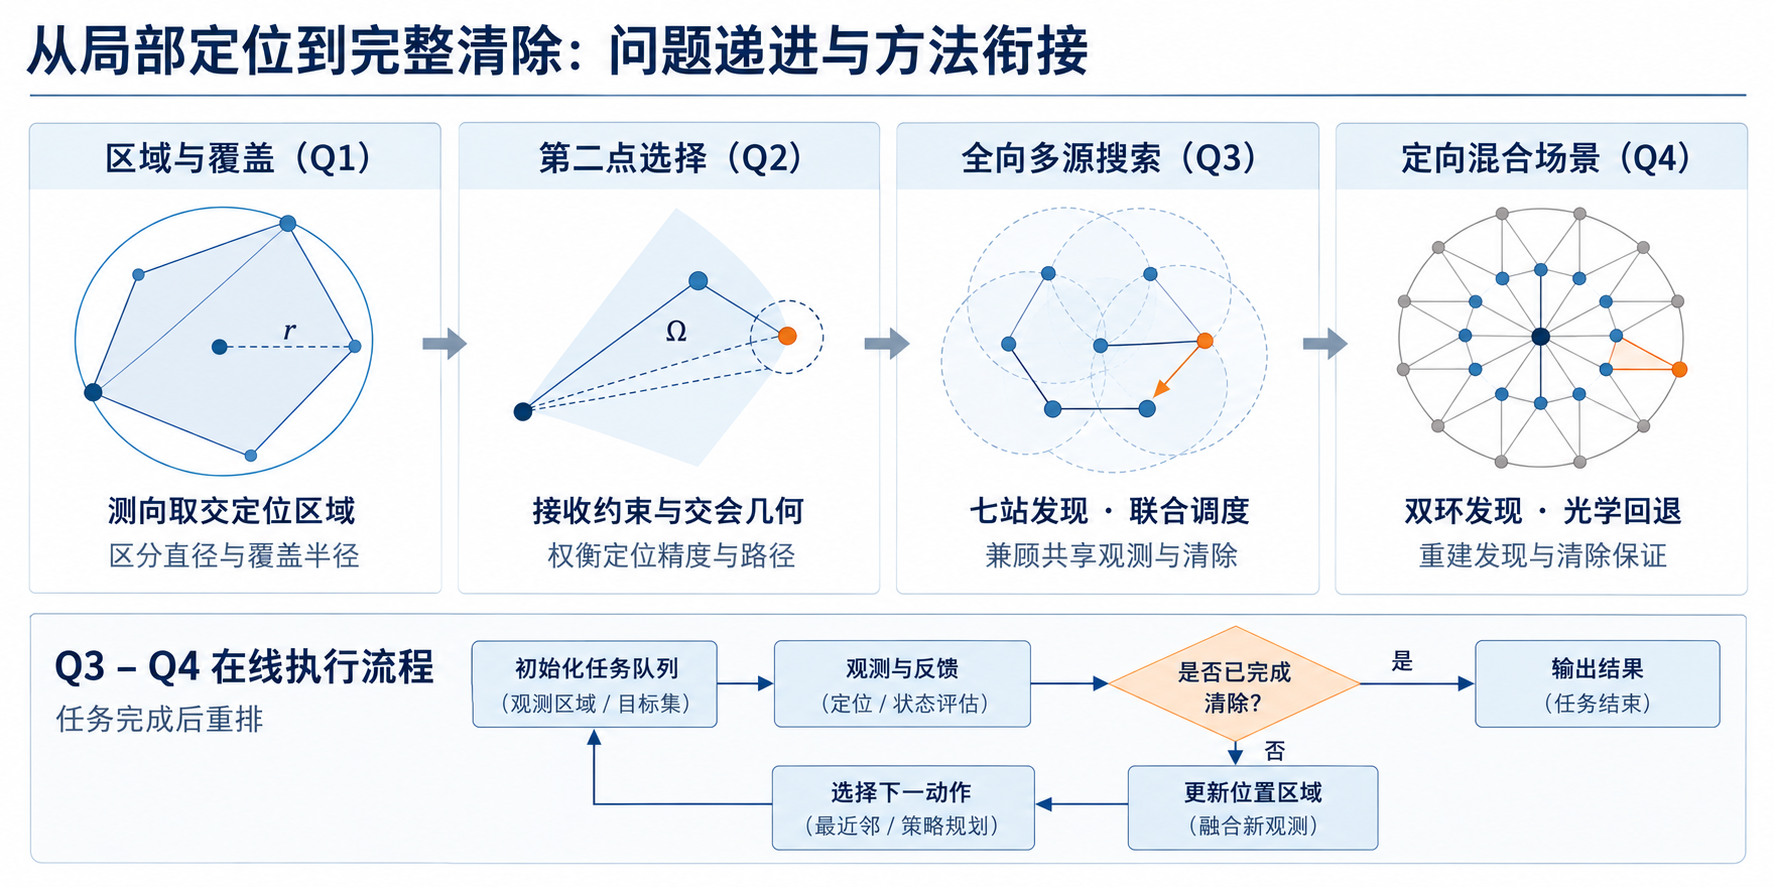
\includegraphics[width=0.88\linewidth]{figures/fig01_overview_optimized.png}
\caption{整体技术路线。上方按Q1至Q4展示方法递进，下方概括Q3与Q4的在线执行反馈。几何小图为非定量示意；流程中的``完成清除''须同时满足正文的停止判据，不能仅凭已知源全部清除就退出。}
\end{figure}

\section{3 模型假设}\label{ux6a21ux578bux5047ux8bbe}

依据题面及接口规则\textsuperscript{\cite{problem,simulator,interface}}，采用以下前提：

\begin{enumerate}
\def\labelenumi{\arabic{enumi}.}
\tightlist
\item
  \textbf{静态与独立。} 单局中源的位置、频道、半径及方向固定，频道互异且信号互不影响。
\item
  \textbf{平面运动。} 移动距离按直线计算；圆域限定源位置，测点可以位于域外。
\item
  \textbf{理想接收。} 接收由距离与发射方向决定，不另设遮挡或随机丢包；光学清除只受距离限制。
\item
  \textbf{有界误差。} 测向误差为±1°，同点同源误差固定，不设概率分布或同点平均降噪。
\item
  \textbf{顺序计时。} 停止后检测，各动作依次执行并分别计时。
\item
  \textbf{公开信息决策。} 策略仅使用位置、频道、观测反馈及题面范围，不读取源真值、实际半径、方向或总数。
\end{enumerate}

\Needspace{18\baselineskip}
\section{4 符号说明}\label{ux7b26ux53f7ux8bf4ux660e}

主要符号及其含义如下；局部辅助量在使用时定义。

\begingroup\small
\begin{longtable}{@{}>{\raggedright\arraybackslash}p{0.28\linewidth} >{\raggedright\arraybackslash}p{\dimexpr0.72\linewidth-2\tabcolsep\relax}@{}}
\caption{主要符号说明}\\
\toprule
符号 & 含义与层级\tabularnewline
\midrule
\endfirsthead
\toprule
符号 & 含义与层级\\
\midrule
\endhead
\(\Omega\) & 半径1800 m的源位置先验圆域\tabularnewline
\(p,S_i,Q\) & 机器人位置、第\(i\)个检测点、候选第二检测点\tabularnewline
\(g_j,r_j,n_j\) & 第\(j\)个源的位置、接收半径及定向发射轴单位向量\tabularnewline
\(\theta_i,\delta\) & 第\(i\)次示向度及当前采用的误差半宽\tabularnewline
\(\delta_{\mathrm{th}},\delta_{\mathrm{num}}\) & 理论误差半宽1°；程序保守误差半宽1.005°\tabularnewline
\(c,N_{\mathrm{src}}\) & 频道编号；一局中的实际源数\tabularnewline
\(L\) & 累计移动距离，单位m\tabularnewline
\(N_{\mathrm{sw}},N_{\mathrm{det}}\) & 实际测向频道切换次数；成功执行的检测调用次数（包括无信号）\tabularnewline
\(N_{\mathrm{opt}},N_{\mathrm{clr}}\) & 光学调用次数；成功清除的不同源数\tabularnewline
\(T,\tau_{\mathrm{clr}},p_{\mathrm{clr}}\) & 总虚拟时间、逐局每源平均时间及清除比例\tabularnewline
\(\mathcal F_1\) & 首次正常测向后，与角度、距离及源域相容的真实初始候选集合\tabularnewline
\(P\) & 仅由测向楔形取交得到的角度定位区域，可能无界\tabularnewline
\(P_c\) & 频道\(c\)当前的保守位置外包，结合源域、距离上界与有效测向\tabularnewline
\(\mathcal C_{\mathrm{rec}}\) & 对所有初始候选源和相容接收半径均保证再次接收的测点集合\tabularnewline
\(\mathcal C_{\mathrm{safe}}\) & 在接收域内进一步满足近距排除与交会角条件的充分候选域\tabularnewline
\(D(P),R(P,q)\) & 区域直径；区域关于指定点\(q\)的覆盖半径，单位m\tabularnewline
\bottomrule
\end{longtable}
\endgroup

这里``外包''允许保留部分实际上不可能的位置，以换取不删去真源的可靠性。因此\(P_c\)不必等于精确可行集合，\(\mathcal C_{\mathrm{rec}}\)也属于测点空间，不能与源位置集合混为一谈。

程序使用\(\delta_{\mathrm{num}}=1.005^\circ\)，在题面的1°误差界上增加两位小数读数可能引入的0.005°舍入量。这是实现中的保守包络，并非题目直接给出的误差范围。下文\(\delta\)泛指当前使用的半宽，解析示例与数值复核分别注明取值。

\section{5 模型建立与求解}\label{ux6a21ux578bux5efaux7acbux4e0eux6c42ux89e3}

本章先建立四问共用的接收条件与计时模型，再分别给出定位区域计算、第二测点选择以及全向和混合源场景的完整搜索清除方法。

\textbf{统一接收模型。} 设目标圆域为\(\Omega=\{x\in\mathbb R^2:\|x\|\le1800\}\)，第\(j\)个源位置为\(g_j\)、接收半径为\(r_j\in[1000,1500]\) m。全向源在\(\|p-g_j\|\le r_j\)时能够接收；对于定向源，若\(n_j\)为其未知发射轴单位向量，则还需满足

\[
\|p-g_j\|\le r_j,\qquad n_j^\mathsf T(p-g_j)\ge0. \tag{1}
\]

发射半平面包含边界。若接口已给出5 m内的近场响应，则可直接光学清除；但距离源很近也不能消除背向不可见性。光学清除仅要求距离不超过20 m，与发射方向无关。因此，无线电接收和光学清除必须按不同条件处理。

\textbf{统一代价与完成指标。}

设累计移动距离为 \(L\)，实际测向频道切换次数为 \(N_{\mathrm{sw}}\)，成功执行的检测调用次数为 \(N_{\mathrm{det}}\)（包括返回无信号的调用），光学调用次数为 \(N_{\mathrm{opt}}\)，不同源成功清除次数为 \(N_{\mathrm{clr}}\)。按照给定计费规则，总虚拟时间为

\[
T=\frac{L}{5}+N_{\mathrm{sw}}+5N_{\mathrm{det}}+3N_{\mathrm{opt}}+2N_{\mathrm{clr}}. \tag{2}
\]

光学调用无论成功与否都花费3 s，成功清除再加2 s；\texttt{/clear} 不切换测向机频道，因此不计入 \(N_{\mathrm{sw}}\)。各动作串行计费，不能用同时执行抵消代价。程序的现实运行时间另行记录，不等于式（2）的虚拟时间。

评价首先要求全部源实际清除且停止条件合法，然后比较 \(T\)。这样可以排除通过漏清或提前退出获得较低时间的策略。题目要求的每源平均时间记为 \(\tau_{\mathrm{clr}}=T/N_{\mathrm{clr}}\)，跨局统计先逐局计算再平均，不用 \(\sum T/\sum N_{\mathrm{clr}}\) 替代。若 \(N_{\mathrm{clr}}=0\)，该指标不定义，该局仍保留为失败记录。

成功清除比例定义为 \(p_{\mathrm{clr}}=N_{\mathrm{clr}}/N_{\mathrm{src}}\)；只有 \(p_{\mathrm{clr}}=1\) 且停止依据合法时才算完整完成。\(N_{\mathrm{src}}\) 由评价器事后核验，策略执行时不能读取。

\FloatBarrier
\subsection{5.1 问题一：交会定位区域的直径计算与圆覆盖判定}\label{ux95eeux9898ux4e00ux4ea4ux4f1aux5b9aux4f4dux533aux57dfux7684ux76f4ux5f84ux8ba1ux7b97ux4e0eux5706ux8986ux76d6ux5224ux5b9a}

\subsubsection{5.1.1 交会定位区域的数学建模}\label{ux4ea4ux4f1aux5b9aux4f4dux533aux57dfux7684ux6570ux5b66ux5efaux6a21}

对于仅给出误差界的观测，集合估计用与误差界相容的集合描述未知量\textsuperscript{\cite{milanese1991}}。本文将这一思想用于测向定位，以各次观测约束的交集表示源的可能位置。

设同一干扰源的 \(n\) 组检测数据为 \(\{(S_i,\theta_i)\}_{i=1}^n\)，其中 \(S_i=(x_i,y_i)^{\mathsf T}\) 为检测点坐标，\(\theta_i\) 为对应示向度，待定位点记为 \(z=(x,y)^{\mathsf T}\)。本问取题面误差半宽 \(\delta=1^\circ\)，以各次测向扇区的交集作为多边形定位区域；源域和接收距离约束在后续各问中另行加入。

第 \(i\) 次测向的两条边界方向为 \(u_i^{\pm}=(\cos(\theta_i\pm\delta),\sin(\theta_i\pm\delta))^{\mathsf T}\)。记二维叉积为 \([a,b]=a_xb_y-a_yb_x\)，则与该次读数相容的位置满足

\[
[u_i^-,z-S_i]\ge0,\qquad [u_i^+,z-S_i]\le0. \tag{3}
\]

式（3）分别限定点位于下边界的左侧和上边界的右侧，两者共同构成张角为 \(2\delta\) 的前向楔形，记为 \(W(S_i,\theta_i,\delta)\)。由于 \(2\delta<180^\circ\)，该表示同时限定了方位误差和前向方向，且适用于示向度跨越 \(0^\circ\) 的情况。

将叉积展开，令两个半平面的行法向量及右端项为

\[
\begin{aligned}
a_{2i-1}&=(\sin(\theta_i-\delta),-\cos(\theta_i-\delta)),
& b_{2i-1}&=a_{2i-1}S_i,\\
a_{2i}&=(-\sin(\theta_i+\delta),\cos(\theta_i+\delta)),
& b_{2i}&=a_{2i}S_i.
\end{aligned}
\]

以 \(a_j\) 为矩阵 \(A\) 的第 \(j\) 行，\(b=(b_1,\ldots,b_{2n})^{\mathsf T}\)，便得到定位区域模型

\[
P=\bigcap_{i=1}^nW(S_i,\theta_i,\delta)
 =\{z\in\mathbb R^2:Az\le b\},\qquad A\in\mathbb R^{2n\times2}.
\]

半平面的交集具有凸性\textsuperscript{\cite{boyd2004}}。观测与误差假设一致时，真实源位于 \(P\) 内；但不同测向的交集可能无界，也可能退化为线段或单点。因此，计算直径前需先判断区域的状态。

\subsubsection{5.1.2 定位区域直径的计算}\label{ux5b9aux4f4dux533aux57dfux76f4ux5f84ux7684ux8ba1ux7b97}

对非空有界的\(P\)，顶点集为\(V(P)=\{v_1,\ldots,v_k\}\)，则

\[
D(P)=\max_{z,w\in P}\|z-w\|
=\max_{1\le a,b\le k}\|v_a-v_b\|. \tag{4}
\]

任意\(z,w\)均为顶点凸组合，三角不等式给出\(\|z-w\|\le\max_{a,b}\|v_a-v_b\|\)；反向不等式由顶点属于\(P\)得到。计算步骤如下。

\begin{enumerate}
\def\labelenumi{\arabic{enumi}.}
\tightlist
\item
  \textbf{判定状态。} 线性规划检查\(Az\le b\)的可行性；为空时直径不定义。分别最小化\(x,-x,y,-y\)，任一无界则\(D(P)=+\infty\)。
\item
  \textbf{恢复顶点。} 枚举全部不平行边界对的交点，保留满足所有约束者并去重；有界区域的每个顶点必在其中。
\item
  \textbf{计算直径。} 比较全部顶点对，输出最大距离及端点；线段取两端距离，单点取0。
\end{enumerate}

除固定次数的二维线性规划外，顶点筛选复杂度为\(O(n^3)\)，直径比较为\(O(n^2)\)。图2算例以\(G=(600,180)\) m、\(S_1=(0,0)\)、\(S_2=(850,-450)\) m和零中心线误差生成读数，得\(D(P)=33.691\) m；详细输入、顶点及计算精度见附录E.1。

\begin{figure}[!htbp]
\centering
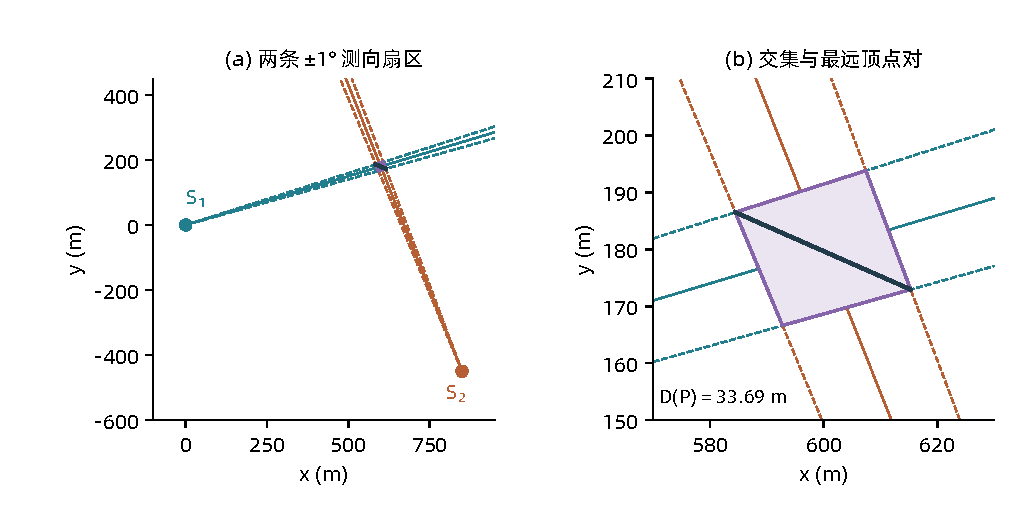
\includegraphics[width=0.76\linewidth]{figures/fig16_bearing_intersection.pdf}
\caption{两次测向定位算例。左图为两个测向扇区，右图放大其交集；黑色线段连接最远顶点对，长度约为33.69 m。}
\end{figure}

\subsubsection{5.1.3 直径圆的覆盖判定}\label{ux76f4ux5f84ux5706ux7684ux8986ux76d6ux5224ux5b9a}

对于非空有界的定位区域 \(P\)，以其直径 \(D\) 为直径的圆不一定能够覆盖整个区域。为判断具体区域是否满足这一性质，取一对直径端点 \(v_a,v_b\)。若半径为 \(D/2\)、圆心为 \(q\) 的圆盘包含 \(P\)，则必须同时包含这两个端点，因而

\[
D=\|v_a-v_b\|\le\|v_a-q\|+\|q-v_b\|\le D.
\]

上式两处不等式均须取等号，故圆心只能是 \(q_D=(v_a+v_b)/2\)。定义区域关于指定点 \(q\) 的覆盖半径为

\[
R(P,q)=\max_{v\in V(P)}\|v-q\|. \tag{5}
\]

圆盘是凸集，包含全部顶点即可包含其凸包 \(P\)。因此，存在直径为 \(D\) 的圆盘覆盖 \(P\) 的充要条件为

\[
R(P,q_D)\le D/2,\qquad q_D=\frac{v_a+v_b}{2}.
\]

图2算例中，\(q_D\approx(599.882,179.731)\) m，且 \(R(P,q_D)=D/2\approx16.845\) m，满足上述判据，因此直径圆可以覆盖整个定位区域。

一般情形则不成立。如图3，取等边三角形顶点 \((0,0)\)、\((39,0)\)、\((19.5,19.5\sqrt3)\)，其直径为39 m。以底边为直径时，圆心为 \((19.5,0)\)，第三顶点距圆心 \(19.5\sqrt3\approx33.775\) m，大于圆半径19.50 m，覆盖判据不成立。由圆心唯一性，改换圆心也无法得到直径为39 m的覆盖圆。该三角形的最小覆盖圆为外接圆，其半径为 \(39/\sqrt3\approx22.52\) m，严格大于 \(D/2\)。附录B.1给出能够产生该三角形的三组合法测向数据。

\begin{figure}[!htbp]
\centering
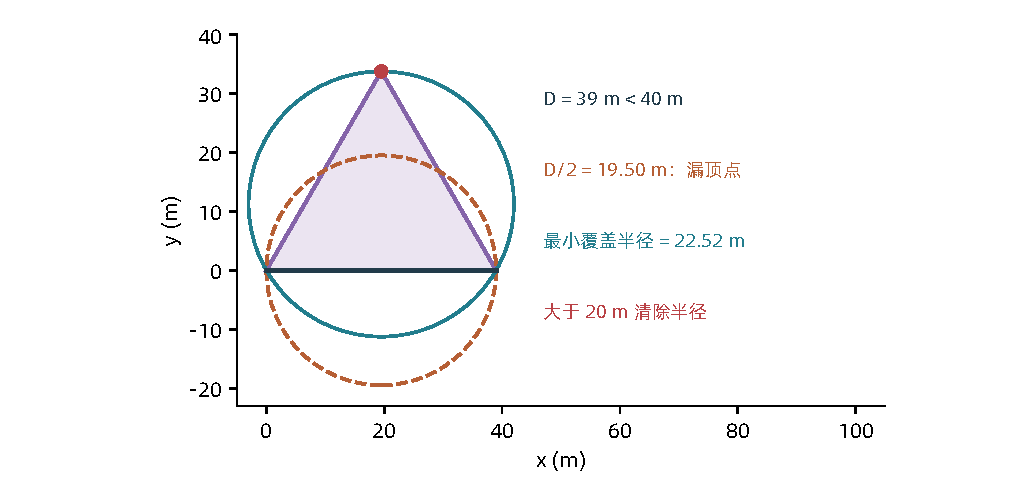
\includegraphics[width=0.78\linewidth]{figures/fig02_diameter.pdf}
\caption{直径圆不能覆盖定位区域的反例。橙色虚线圆以三角形底边为直径，半径为19.50 m，未覆盖上方顶点；蓝色实线圆为最小覆盖圆，半径约为22.52 m。}
\end{figure}

这一结论也给出后续清除的判断依据：对于维护的位置外包 \(P_c\)，若 \(R(P_c,q)\le20\) m，则在 \(q\) 可以保证光学清除；仅有 \(D(P_c)\le40\) m 不足以作出该保证。

\FloatBarrier
\subsection{5.2 问题二：第二检测点的选择}\label{ux95eeux9898ux4e8cux7b2cux4e8cux68c0ux6d4bux70b9ux7684ux9009ux62e9}

本问只给出首次检测点及示向度，尚不能确定源距，也没有给出源位置或测向误差的概率分布。本文将``较好的定位效果''具体化为：在保证第二次获得正常示向度、避免近共线交会的条件下，尽量减小两次测向定位区域的最坏直径。移动时间作为候选方案的附加比较指标，第三问再以完整清除时间为目标安排动作。

\subsubsection{5.2.1 测向几何关系}\label{ux6d4bux5411ux51e0ux4f55ux5173ux7cfb}

设首测点为 \(S\)，测得示向度为 \(\theta\)，误差半宽为 \(\delta\)。以示向方向为局部横轴，定义正交单位向量

\[
u=(\cos\theta,\sin\theta),\qquad
v=(-\sin\theta,\cos\theta).
\]

任一与首次读数相容的候选源 \(G\) 和待选第二测点 \(Q\) 可表示为

\[
G=S+r(\cos\alpha\,u+\sin\alpha\,v),\qquad
Q=S+au+bv.
\]

其中，\(r=\|G-S\|\) 为首测点到源的距离，\(\alpha\) 为真实方向相对示向度的偏差；\(a,b\) 分别为第二测点沿示向方向和法向的位移。正常示向度意味着 \(5<r\le1500\) m 且 \(|\alpha|\le\delta\)。结合源位置先验圆域 \(\Omega\)，首次候选位置集合为

\[
\mathcal F_1=\{S+r(\cos\alpha\,u+\sin\alpha\,v):
5<r\le1500,\ |\alpha|\le\delta\}\cap\Omega.
\]

记 \(d_2=\|G-Q\|\)，\(\varphi\in[0,\pi]\) 为向量 \(G-S\) 与 \(G-Q\) 的夹角。将两条视线的锐交会角定义为 \(\beta=\min(\varphi,\pi-\varphi)\)。当 \(\beta\) 接近0时，两次测向近共线，角度误差会形成狭长甚至无界的交集；因此应同时考虑第二点是否仍能接收和交会角是否足够大。

图4给出几何关系及两个反例。若源为 \((1500,0)\) m、接收半径为1500 m，从首测点 \((0,0)\) 横移到 \((0,500)\) 后，源距增至1581.14 m，发生失联；前移到 \((500,0)\) 虽仍能接收，却与源保持共线，不能保证纯角度交集有界。这说明单独增加横向位移或沿示向度靠近，都不足以构成完整的第二测点选择策略。

\begin{figure}[!htbp]
\centering
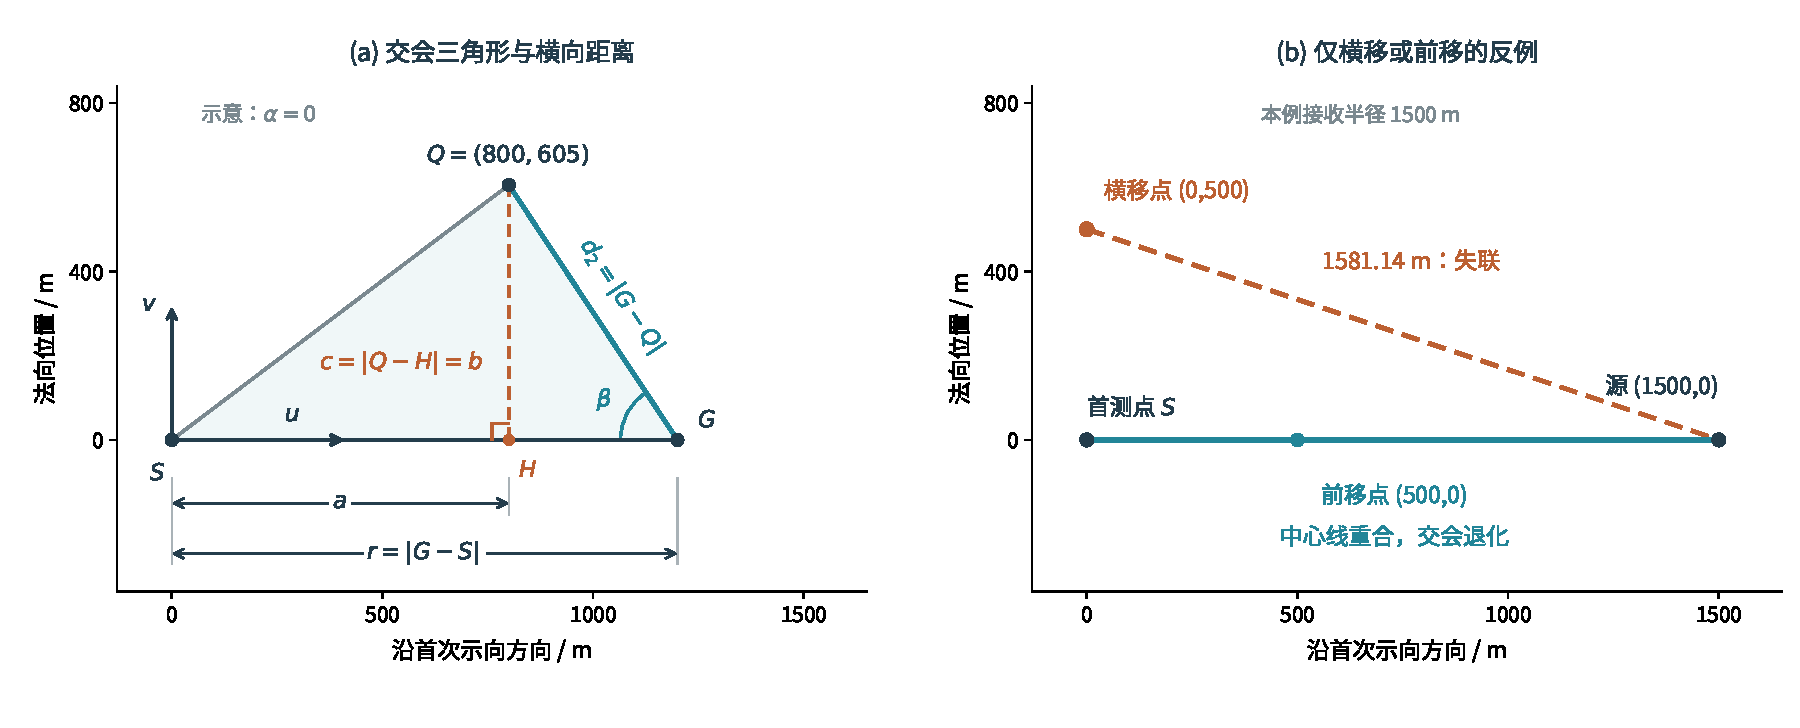
\includegraphics[width=0.90\linewidth]{figures/fig03_q2_failures.pdf}
\caption{第二测点的几何关系与典型反例。（a）图示取 \(\alpha=0\)、\(b>0\)，\(H\) 为 \(Q\) 在真实视线 \(SG\) 上的垂足，此时 \(c=b\) 且 \(\sin\beta=c/d_2\)；（b）横移可能超出接收范围，前移可能造成交会退化。坐标均为构造示例，不代表搜索轨迹。}
\end{figure}

\subsubsection{5.2.2 信号接收条件}\label{ux4fe1ux53f7ux63a5ux6536ux6761ux4ef6}

首次成功接收说明真实接收半径\(R_G\ge r\)，结合\(R_G\in[1000,1500]\)，其相容最小值为\(\max(1000,r)\)。因此，对固定候选源\(G\)，第二点保证接收的充要条件为

\[
\|Q-G\|\le\max(1000,\|G-S\|). \tag{6}
\]

对全部\(G\in\mathcal F_1\)取交，得\(\mathcal C_{\mathrm{rec}}=\bigcap_{G\in\mathcal F_1}B(G,\max(1000,\|G-S\|))\)，其中\(B\)为闭圆盘。为得到不依赖首测位置的通用策略，使用不经源域裁剪的闭合扇形外包

\[
\mathcal F_0=\{S+r(\cos\alpha\,u+\sin\alpha\,v):
5\le r\le1500,\ |\alpha|\le\delta\}\supseteq\mathcal F_1.
\]

令\(\ell=\sqrt{a^2+b^2}\)、\(t(\alpha)=a\cos\alpha+b\sin\alpha\)，则\(d_2^2=\ell^2+r^2-2rt(\alpha)\)。近段\(r\in[5,1000]\)的距离平方为凸函数，只需检查两端；远段\(r\in[1000,1500]\)由\(r=1000\)条件控制。可行性要求\(a\ge0\)，最不利方向投影为\(h=\min t=a\cos\delta-|b|\sin\delta\)，故

\[
\boxed{a\ge0,\qquad \ell^2-10h+25\le10^6,\qquad
\ell^2\le2000h.} \tag{7}
\]

式（7）对\(\mathcal F_0\)充要，对裁剪后的\(\mathcal F_1\)可能偏保守；它也排除了\(a=0,b\ne0\)的纯横移。完整分段推导见附录E.2。

\subsubsection{5.2.3 交会角约束}\label{ux4ea4ux4f1aux89d2ux7ea6ux675f}

为获得正常读数并避免共线，进一步要求\(d_2>5\) m、锐交会角\(\beta\ge20^\circ\)。图4(a)中第二测点到真实视线的垂距为\(c=|b\cos\alpha-a\sin\alpha|\)，且\(\sin\beta=c/d_2\)。定义

\[
\begin{aligned}
c_{\min}&=|b|\cos\delta-a\sin\delta,\\
M^2&=\max\{\ell^2+25-10h,\ \ell^2+1500^2-3000h\}.
\end{aligned}
\]

由\(c\ge c_{\min}\)及\(d_2\le M\)，以下条件足以保证正常接收距离与交会角：

\[
\boxed{c_{\min}>5,\qquad c_{\min}\ge M\sin20^\circ.} \tag{8}
\]

于是\(\mathcal C_{\mathrm{safe}}=\{S+au+bv:\text{式（7）、（8）成立}\}\)，其关于示向轴对称，见图5。\(M\)是最大第二源距；式（8）为充分条件，20°是设计参数，均不宣称最优。真实源保证交集非空，且\(20^\circ-2\delta>2\delta\)（\(\delta=1^\circ\)或\(1.005^\circ\)），两楔形无共同非零延伸方向，故交集有界。

\begin{figure}[!htbp]
\centering
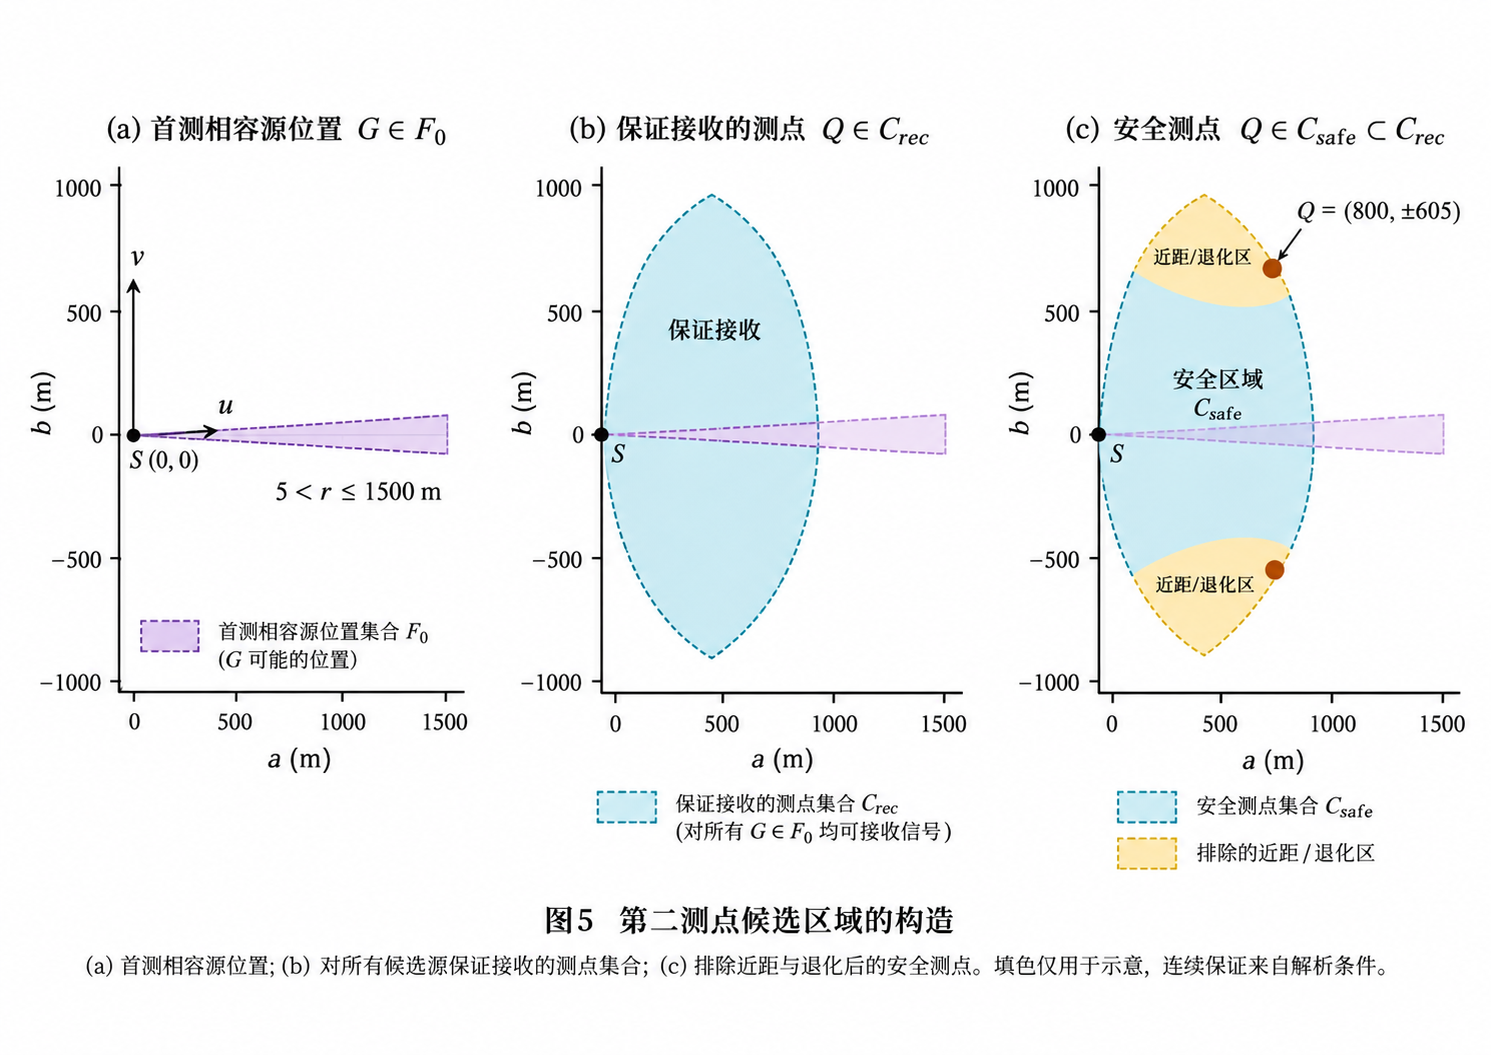
\includegraphics[width=0.90\linewidth,trim={0 175bp 0 65bp},clip]{figures/fig04_q2_region_optimized.png}
\caption{第二测点候选区域的构造示意。（a）首次测向的相容源位置；（b）保证接收的测点集合；（c）安全测点筛选及推荐镜像点。填色仅示意集合关系，不作为边界或点归属的数值判据；安全区域严格由式（7）和式（8）共同确定，轴线上退化测点不属于安全区域。}
\end{figure}

\subsubsection{5.2.4 优化模型及求解}\label{ux4f18ux5316ux6a21ux578bux53caux6c42ux89e3}

对候选点\(Q\)、相容源\(G\)和第二次误差\(\varepsilon_2\)，读数为\(\theta_2=\arg(G-Q)+\varepsilon_2\)，定位区域为\(P(Q;G,\varepsilon_2)=W(S,\theta,\delta)\cap W(Q,\theta_2,\delta)\)。首次误差已由\(\alpha\)确定，不再独立设置。建立最坏定位直径模型：

\[
\begin{aligned}
J_0(Q)&=\sup_{G\in\mathcal F_0,\ |\varepsilon_2|\le\delta}
D(P(Q;G,\varepsilon_2)),\\
Q^*&\in\operatorname*{arg\,min}_{Q\in\mathcal C_{\mathrm{safe}}}J_0(Q).
\end{aligned} \tag{9}
\]

决策变量为\((a,b)\)，只以定位直径为目标；\(P\)沿用第一问的纯角度交集。以\(\mathcal F_0\)代替\(\mathcal F_1\)使策略通用且可能保守，有限场景仅近似上确界。求解分三步：

\begin{enumerate}
\def\labelenumi{\arabic{enumi}.}
\tightlist
\item
  \textbf{粗网格筛选。} 令\(S=0,\theta=0,\delta=1^\circ\)，仅搜\(b>0\)。取\(a=0,50,\ldots,1000\) m，\(b=50,100,\ldots,1000\) m，以解析式（7）、（8）筛选。源距51点、两个误差维度各5点组成1275场景，逐一求交并取最大直径。
\item
  \textbf{局部加密。} 优先最小采样直径，同值时依次比较移动距离、\(a,b\)；在粗选点周围±50 m内以5 m步长加密。粗选\((800,600)\) m对应134.976 m，加密得到\((800,605)\) m及134.284 m。
\item
  \textbf{复核与还原。} 增加至\(301\times11\times11=36,421\)场景，推荐点最大直径在所报精度下不变；按\(Q=S+au+bv\)还原。再以±1.005°复核既定8点及镜像，不重新搜索坐标。
\end{enumerate}

每个场景的半平面数固定，\(N_Q\)个候选、\(K\)个场景的评分复杂度为\(O(N_QK)\)。采样端点及评价次数见附录E.3。

\subsubsection{5.2.5 结果分析}\label{ux7ed3ux679cux5206ux6790}

以下列出1.005°包络下三个代表候选。锐交会角下界按 \(\arcsin(c_{\min}/M)\) 计算，各点及其镜像均通过式（7）、式（8）；全部8点的精度与时间数据见附录B.2。

\begin{table}[H]
\centering\small
\caption{第二测点代表候选的解析条件与数值结果}
\begin{tabular}{@{}lrrr@{}}
\toprule
局部偏移 \((a,b)\)/m & 交会角下界/° & 采样最大直径/m & 移动与检测/s\tabularnewline
\midrule

(500,500) & 25.767 & 236.082 & 146.421\tabularnewline
(850,450) & 27.025 & 154.298 & 197.354\tabularnewline
(800,605) & 36.258 & 135.026 & 205.602\tabularnewline
\bottomrule
\end{tabular}
\end{table}

推荐点满足\(c_{\min}=590.875\) m、\(M=999.078\) m及两组解析条件。其他候选的\(M>1000\) m不等于失联，接收须按式（7）判断。

因此，以采样最坏定位直径为准，本文保留的第二测点推荐为

\[
\boxed{\begin{aligned}
Q^{\pm}&=S+800u\pm605v\\
&=S+800(\cos\theta,\sin\theta)
\pm605(-\sin\theta,\cos\theta).
\end{aligned}}
\]

两镜像在完整扇形模型下等价；利用源域裁剪或后续任务后应另行比较。第二次测向后按第一问更新区域，仍以20 m覆盖判据决定清除。

图6展示固定候选库内的定位精度与移动代价。相对 \((500,500)\)，推荐点将采样最大直径降低42.81\%，但多花59.18 s。表中计时为 \(\ell/5+5\)：追踪同一频道无需切频，尚未计入后续定位与清除。该比较说明第二问的精度推荐不能直接等同于第三问的最快清除动作。

\begin{figure}[!htbp]
\centering
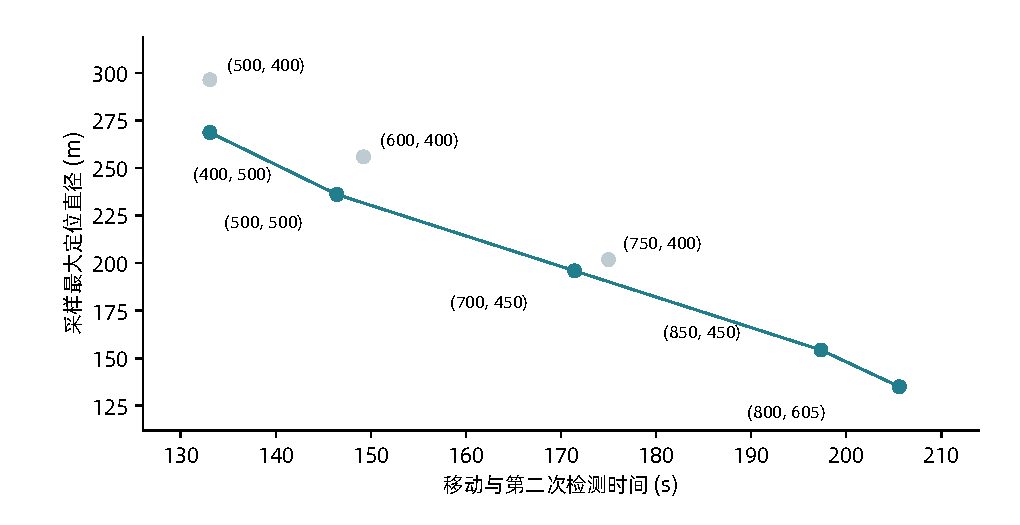
\includegraphics[width=0.88\linewidth]{figures/fig05_q2_tradeoff.pdf}
\caption{固定候选库的精度与移动代价比较。展示8个上侧候选，镜像具有相同指标；蓝色为库内非支配点，灰色为被支配点，橙色为保留推荐点。纵轴为36,421个场景中的最大直径，连线仅连接库内非支配点。}
\end{figure}

候选的接收及交会保证来自式（7）、式（8）；134.284 m和135.026 m分别是1°、1.005°条件下的有限场景最大值。加密后结果一致支持当前数值计算的稳定性，但不排除网格之间存在更差情形，也不证明候选搜索或20°阈值全局最优。第三问将继续使用这些几何条件，并把测量、移动和清除放入完整任务中评价。

\FloatBarrier
\subsection{5.3 问题三：全向干扰源的搜索与清除}\label{ux95eeux9898ux4e09ux5168ux5411ux5e72ux6270ux6e90ux7684ux641cux7d22ux4e0eux6e05ux9664}

第三问要求在源数、位置和接收半径未知的条件下完成全部清除，并尽量缩短式（2）给出的总时间。为此，将行动划分为两类任务：搜索任务负责发现未知频道，源服务任务负责将一个已知源定位并清除。以公开观测形成的位置区域作为决策依据，在可靠测向与清除约束下安排任务顺序，形成``区域更新---动作选择---任务执行---完成核验''的在线算法。

\subsubsection{5.3.1 位置区域的建立与更新}\label{ux4f4dux7f6eux533aux57dfux7684ux5efaux7acbux4e0eux66f4ux65b0}

在第\(t\)次任务决策时，记机器人位置为\(p_t\)，已发现频道集合为\(\mathcal D_t\)，已成功清除频道集合为\(\mathcal C_t\subseteq\mathcal D_t\)，未完成搜索站的编号集合为\(\mathcal S_t\)。搜索采用七个固定站，其坐标及覆盖证明见第5.3.4节。每个已知未清频道\(c\)维护候选位置区域\(P_c\)、最新示向度\(\theta_c\)及已检测位置记录；每个未知频道保留各搜索站的无信号记录。发现和清除集合仅根据实际反馈更新，隐藏源坐标不参与任务决策。

设频道\(c\)首次正常测向的位置为\(S_c\)、读数为\(\theta_c^{(0)}\)。以\(\widehat B_{32}(s,r)\)表示圆盘\(B(s,r)\)的32个外切支持半平面之交，则初始位置区域及后续更新为

\[
\begin{aligned}
P_c^{(0)}&=\widehat B_{32}(0,1800)\cap\widehat B_{32}(S_c,1500)
\cap W(S_c,\theta_c^{(0)},\delta),\\
P_c^{(k+1)}&=P_c^{(k)}\cap W(s,\theta,\delta).
\end{aligned}
\]

其中\((s,\theta)\)为新获得的正常测向，程序取\(\delta=1.005^\circ\)。1500 m是首次接收给出的距离上界；采用外切近似，可保留圆周附近的合法位置。由于每个加入的约束均包含真实源\(g_c\)，有

\[
g_c\in P_c^{(k+1)}\subseteq P_c^{(k)}.
\]

因此，位置区域随有效观测逐步缩小，且始终保留真实源。后续无信号不用于裁剪这一多边形；在保证接收的位置出现无信号时，按模型或执行异常处理。

为从区域生成测点，沿最新示向方向建立正交基\(u_c=(\cos\theta_c,\sin\theta_c)^{\mathsf T}\)、\(v_c=(-\sin\theta_c,\cos\theta_c)^{\mathsf T}\)。对\(e\in\{u_c,v_c\}\)，记\(\ell_{c,e}=\min_{x\in P_c}e^{\mathsf T}x\)、\(h_{c,e}=\max_{x\in P_c}e^{\mathsf T}x\)，则该方向下包围盒的中心及其覆盖半径为

\[
q_c=\frac12\sum_{e\in\{u_c,v_c\}}(\ell_{c,e}+h_{c,e})e,
\qquad R_c=R(P_c,q_c).
\]

后文的区域中心均指\(q_c\)，即沿最新示向方向旋转的包围盒中心。由式（5）的顶点覆盖判据，对于任意候选测点\(q\)，

\[
\begin{aligned}
R(P_c,q)<1000\ \mathrm m&\quad\Longrightarrow\quad\text{保证接收到该全向源},\\
R(P_c,q)<20\ \mathrm m&\quad\Longrightarrow\quad\text{保证在该点清除该源}.
\end{aligned}
\]

这两个条件分别把题目的最小接收半径和光学清除半径转化为可计算约束。程序逐顶点核验并预留数值余量；实际清除成功后才更新\(\mathcal C_t\)。

\subsubsection{5.3.2 测点选择与定位清除}\label{ux6d4bux70b9ux9009ux62e9ux4e0eux5b9aux4f4dux6e05ux9664}

\textbf{（1）局部测点选择。} 服务频道\(c\)时，先计算\(q_c\)与\(R_c\)。若\(R_c<20\) m，则前往\(q_c\)清除；否则，在本次服务的首轮局部测向中考察两个横向候选点

\[
q_c^\pm=q_c\pm\sqrt{20R_c}\,(-\sin\theta_c,\cos\theta_c). \tag{10}
\]

垂直于示向方向的位移用于形成视差，偏移尺度中的20表示清除半径20 m。先筛除不满足接收约束的点，再从剩余候选中选取距当前位置最近者；若两点均不满足条件，则使用\(q_c\)。后续轮次在更新后的包围盒中心测向，每轮均先检查清除和接收条件。由于此前可能已有共享观测，服务首轮不一定对应该源的第二次测向。式（10）是固定的几何启发式，其效率由第6.2节的实验评价。

\textbf{（2）中心测量的收缩性质。} 若当前\(P\subseteq B(q,R)\)，在\(q\)得到半宽\(\delta<30^\circ\)的正常方位后，新的区域记为\(P^+\)，则

\[
D(P^+)\le\max\{R,2R\sin\delta\}=R,
\qquad R(P^+,q^+)\le\frac{R}{\sqrt2},
\]

其中\(q^+\)为新区域的包围盒中心。前一不等式来自半径\(R\)圆盘与前向楔形的交集：任意两点的径向距离在\([0,R]\)内，最远距离在径向端点组合中取得，最大值为\(\max\{R,2R\sin\delta\}\)。后一不等式利用包围盒两边长均不超过区域直径，其半对角线不超过\(R/\sqrt2\)。因此，在实数几何模型和正常测向条件下，连续中心测量使覆盖半径按不超过\(1/\sqrt2\)的因子收缩，有限次后可达到清除阈值。

\textbf{（3）有限回退。} 为处理同点重复测量和数值停滞，每个源服务至多进行16轮局部迭代。若迭代结束仍未清除，或下一测点已对该频道检测过，则沿最新示向方向划分当前包围盒，形成边长不超过28 m的网格，并依次前往格心尝试清除。每格内任一点距格心至多\(14\sqrt2<20\) m，故含真源的格必被覆盖。若测向返回5 m内的近场提示，则直接在当前位置清除。接收或清除反馈矛盾、网格耗尽仍未成功时，报告未完成。

图7展示三次测向的区域收缩：中心覆盖半径降至10.66 m后满足清除条件。该教学算例的坐标、读数及固定轴计算口径见附录E.1。

\begin{figure}[!htbp]
\centering
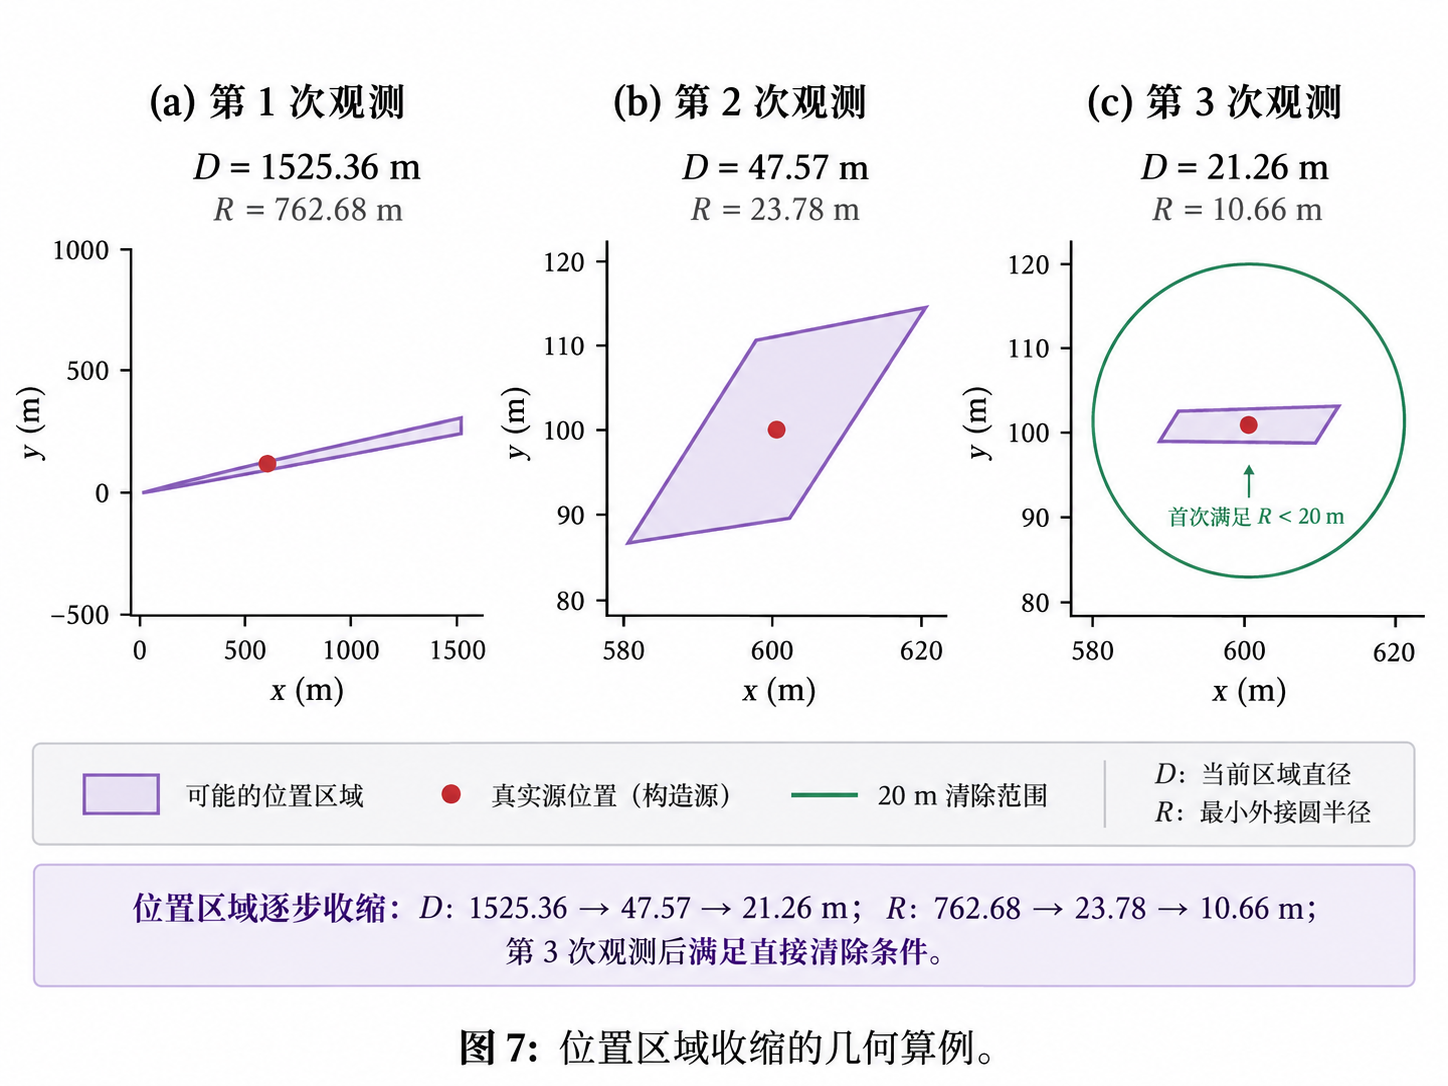
\includegraphics[width=0.92\linewidth,trim={0 90bp 0 45bp},clip]{figures/fig17_shrink_optimized.png}
\caption{位置区域收缩的几何算例。各子图分别放大当前区域，坐标尺度不同；红点为构造源，绿色圆表示20 m清除范围。图中R的数值按固定坐标轴包围盒中心的覆盖半径计算，图内``最小外接圆半径''应按此口径理解；实际策略按最新示向方向旋转包围盒。图示并非实测轨迹，不表示每个源均需三次测量。}
\end{figure}

\subsubsection{5.3.3 观测共享与任务排序}\label{ux89c2ux6d4bux5171ux4eabux4e0eux4efbux52a1ux6392ux5e8f}

\textbf{（1）共享观测的选择条件。} 主目标的一次局部测向返回正常示向度后，在当前位置\(p\)依次检查其他已知未清频道\(j\)。仅对尚未在\(p\)检测、当前\(R_j>20\) m且满足\(R(P_j,p)<1000\) m的频道，进一步判断观测的收缩价值。

由\(P_j\)在\(p\)所见的真实方位范围向两侧扩展误差半宽\(\delta\)，得到可能返回的示向度区间；当\(p\in P_j\)时，保守取完整\(360^\circ\)。将该区间完整分为16段，记第\(\ell\)段的中点为\(m_\ell\)、半宽为\(h_\ell\)，构造后验外包

\[
\widetilde P_{j\ell}=P_j\cap W(p,m_\ell,\delta+h_\ell).
\]

对每个非空\(\widetilde P_{j\ell}\)，沿\(m_\ell\)方向计算包围盒中心\(\widetilde q_{j\ell}\)。仅在满足

\[
\max_{\ell:\,\widetilde P_{j\ell}\ne\varnothing}
R(\widetilde P_{j\ell},\widetilde q_{j\ell})
\le\max(20,R_j/2)
\]

时执行共享检测。对该段内任意实际读数\(\theta\)，有\(W(p,\theta,\delta)\subseteq W(p,m_\ell,\delta+h_\ell)\)，因此判据覆盖全部可能读数。它保证每一种后验均存在满足阈值的覆盖圆，但不保证按实际读数重新旋转的包围盒半径严格减半，也不直接保证整局省时。

共享结果用于收缩其他源的区域，近场反馈则可顺便清除该源。随后继续完成当前主目标的服务，未补测或尚未清除的源留在任务集合中。普通搜索站只检测未知频道，不重复扫描全部已知源。

\textbf{（2）任务访问顺序。} 将未完成搜索站和已知未清源组成任务集合

\[
\mathcal J_t=\{\operatorname{scan}(k):k\in\mathcal S_t\}
\cup\{\operatorname{serve}(c):c\in\mathcal D_t\setminus\mathcal C_t\}.
\]

搜索任务的代表点为站点坐标，源服务任务的代表点为当前\(q_c\)。记这些点为\(z_1,\ldots,z_K\)，访问顺序为排列\(\pi\)，则滚动排序采用的开放路径目标为

\[
L_t(\pi)=\|p_t-z_{\pi_1}\|
+\sum_{i=1}^{K-1}\|z_{\pi_i}-z_{\pi_{i+1}}\|.
\]

借鉴旅行商问题的局部交换改进思想\textsuperscript{\cite{croes1958}}，本文按以下步骤近似求解开放路径问题：分别以各任务为首项，按最近邻规则生成完整路线；对每条路线用2-opt反转局部访问顺序，只接受严格缩短\(L_t\)的调整，直至不能继续改善；在所得路线中选择最短者，并执行其首项任务。由于任务结束后不要求返回起点，目标中不包含返程边。

完成整站必要扫描或当前源的定位清除后，再依据最新反馈重建\(\mathcal J_t\)并排序，如图8所示。任务内部的观测更新位置区域，但不立即切换主目标。\(L_t\)仅计算任务代表点间的移动距离，未完整计入源服务内部行程、检测费用和提前发现第16个源的价值；因此该求解过程是整局时间目标的启发式近似。

\begin{figure}[!htbp]
\centering
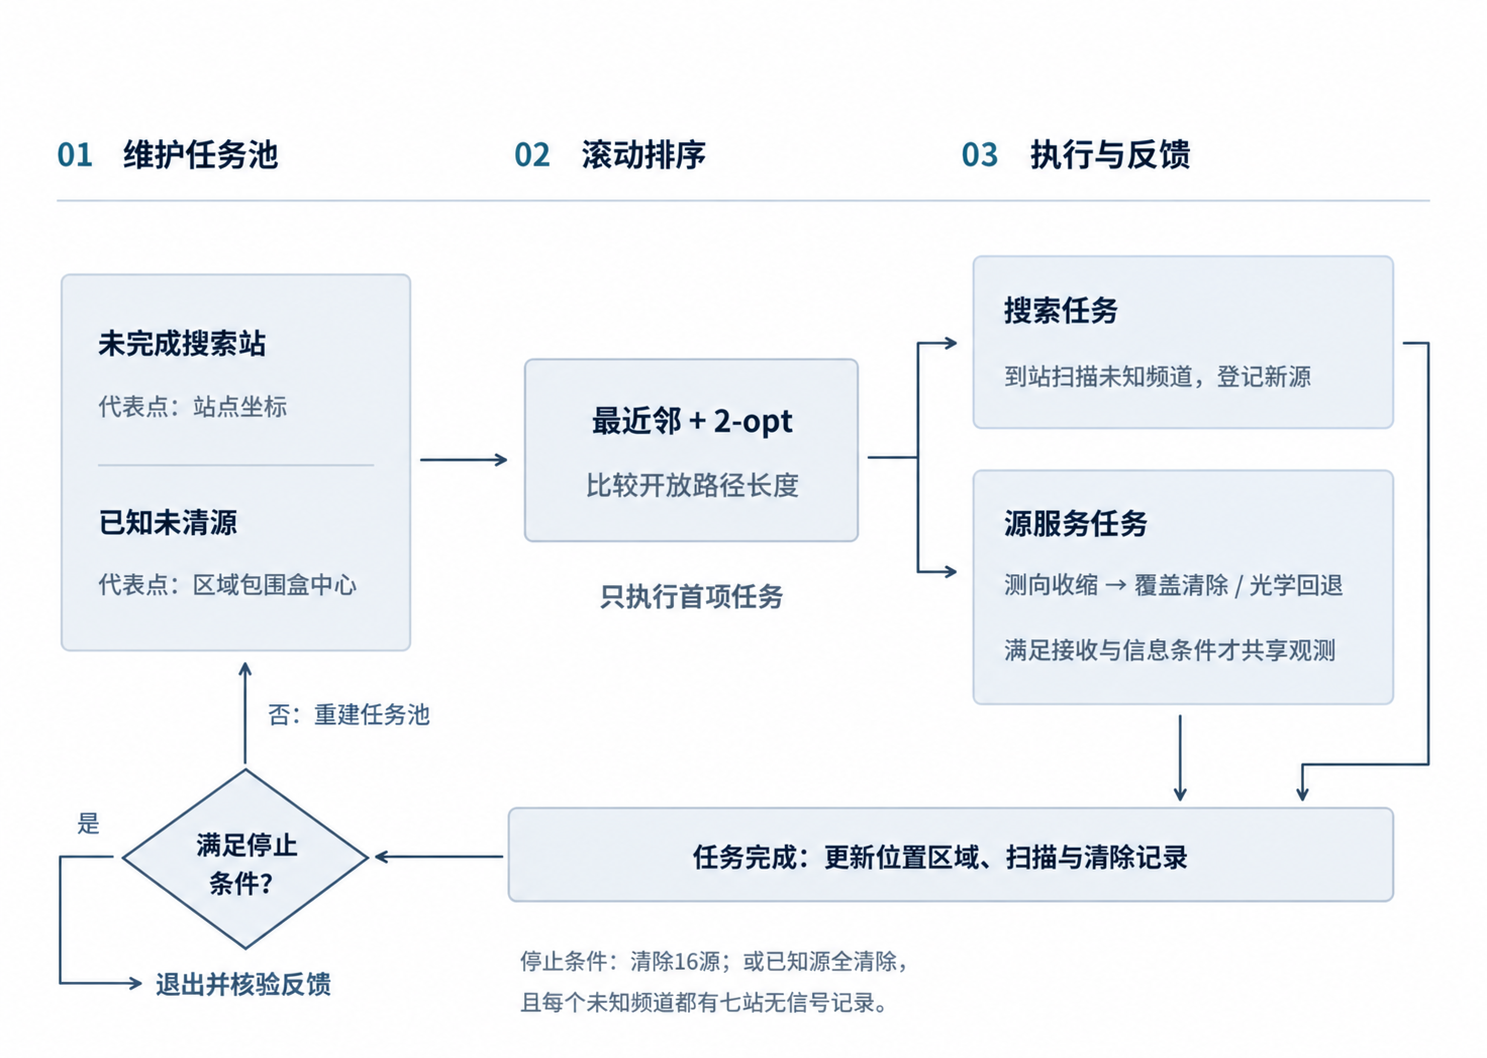
\includegraphics[width=0.84\linewidth,trim={0 25bp 0 105bp},clip]{figures/fig06_q3_algorithm_optimized.png}
\caption{Q3搜索与服务的调度流程。两类任务进入同一任务池，按代表点之间的开放路径长度排序，每次只执行首项任务。搜索与源服务为两种执行分支；共享观测须满足接收与信息条件，清除依据20 m覆盖条件或有限光学回退。任务完成后更新记录、核验停止条件，未满足时重建任务池并重排。}
\end{figure}

图9以三源教学场景示意交错访问，整局收益由第6章验证。

\begin{figure}[!htbp]
\centering
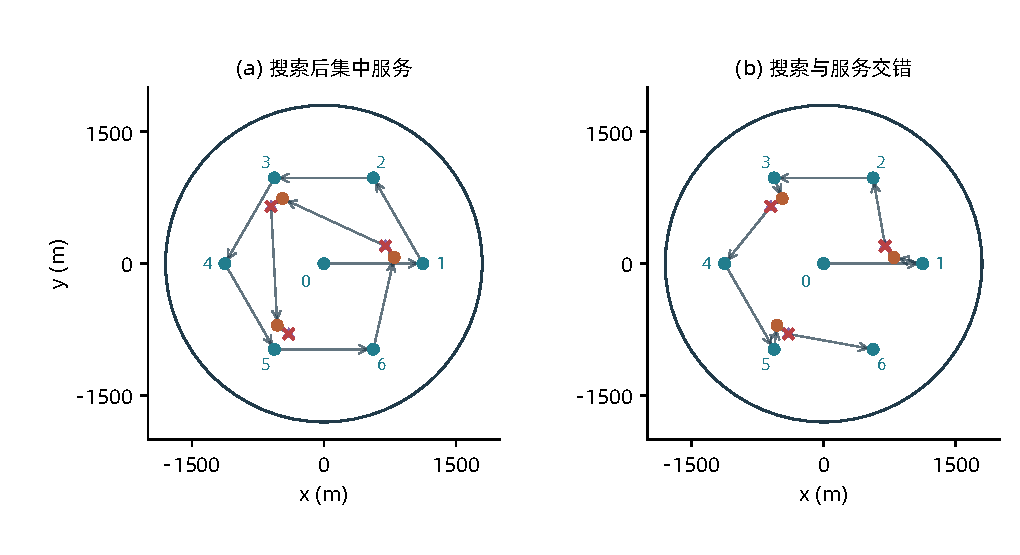
\includegraphics[width=0.88\linewidth]{figures/fig18_route_example.pdf}
\caption{三源教学场景中的任务顺序对比。蓝点为七个搜索站，橙点为后续测向点，红叉为构造源，紫色区域表示定位任务。左图先搜索后服务，右图交错执行；轨迹和区域均为流程示意，源数不符合正式场景要求，也不代表实验基线或性能结果。}
\end{figure}

\FloatBarrier
\subsubsection{5.3.4 搜索站布设与算法流程}\label{ux641cux7d22ux7ad9ux5e03ux8bbeux4e0eux7b97ux6cd5ux6d41ux7a0b}

\textbf{（1）七站发现覆盖。} 固定搜索站为原点和半径1125 m圆周上的六个等角站，其坐标可写为

\[
s_0=(0,0),\qquad
s_{k+1}=1125\bigl(\cos(k\pi/3),\sin(k\pi/3)\bigr),
\quad k=0,\ldots,5.
\]

原点覆盖半径900 m的内圈。外圈任一点与最近圆周站的角距不超过30°；到该站的距离平方关于源的径向距离为凸函数，在\([900,1800]\)上的最大值可由两端点控制。因此整个源域到最近站的距离满足

\[
\max\left\{900,\max_{r\in\{900,1800\}}
\sqrt{r^2+1125^2-2r\cdot1125\cos30^\circ}\right\}
\approx999.11<1000\ \mathrm{m}. \tag{11}
\]

每个全向源因而至少能在一站被接收。若一个未知频道在七站均无信号，就可排除圆域内存在该频道源的可能。1125 m是在保持覆盖的同时缩短固定搜索行程的选择，与历史1500 m方案的比较见附录B.3。

\begin{figure}[!htbp]
\centering
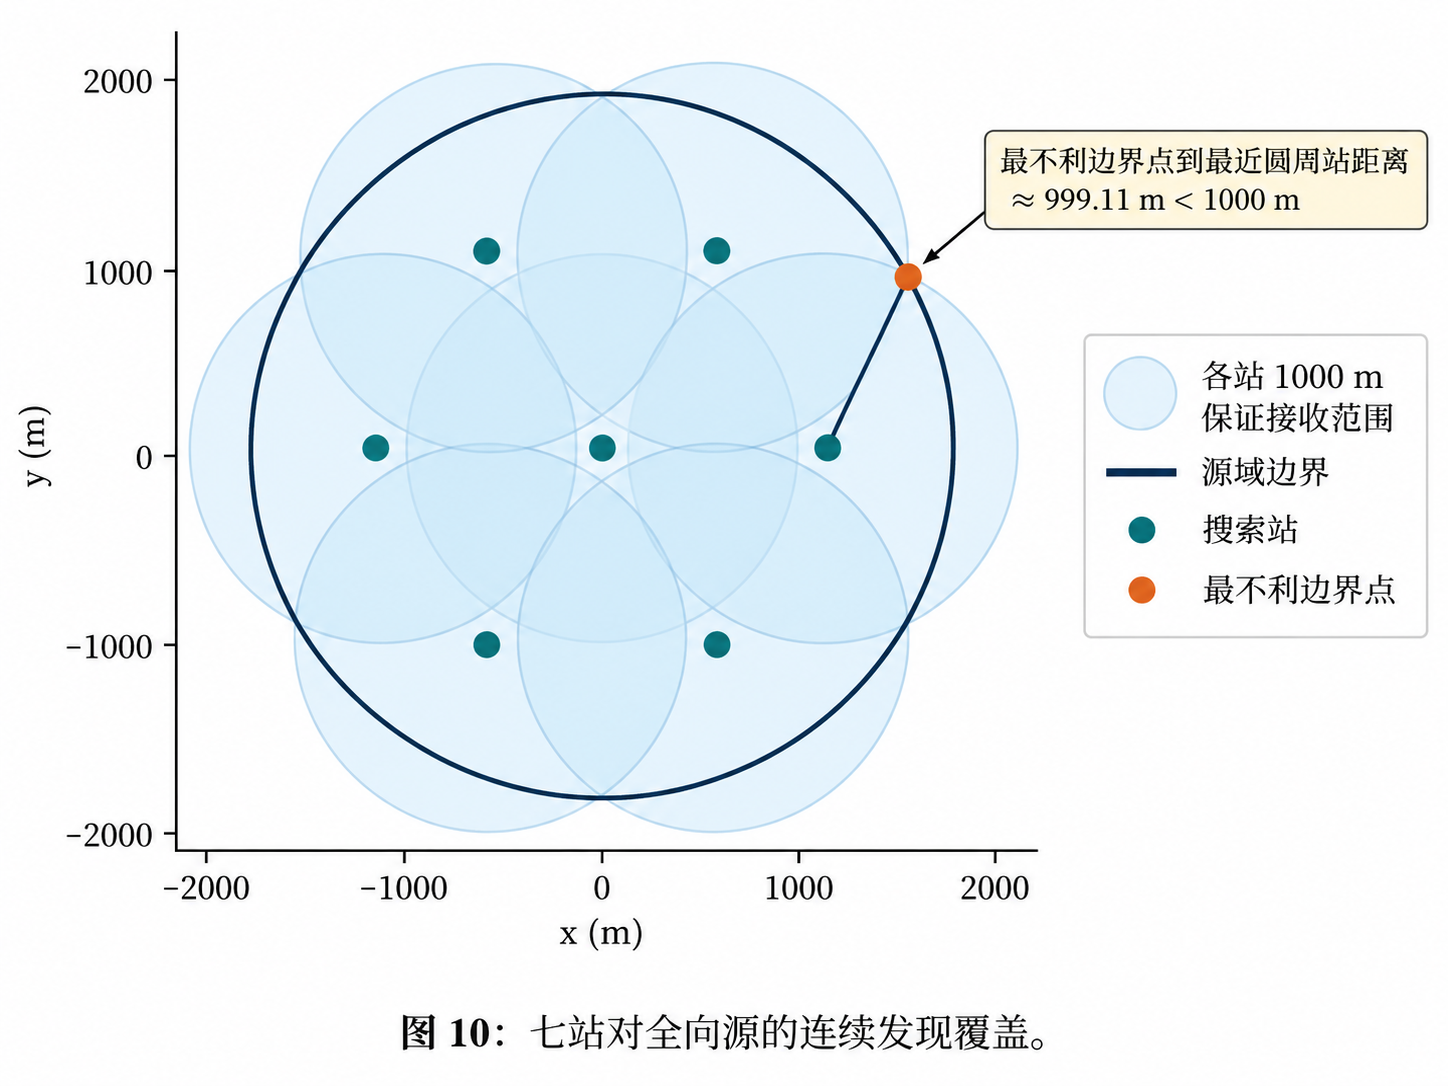
\includegraphics[width=0.70\linewidth,trim={0 110bp 0 0},clip]{figures/fig07_q3_cover_optimized.png}
\caption{七站对全向源的连续发现覆盖示意。浅蓝圆盘为各站1000 m的保证接收范围，深色圆为源域边界，橙点标示最不利边界位置。距离约999.11 m的数值由式（11）计算，示意坐标不用于量取距离；穿插源服务任务时仍保留各频道的实际扫描记录。}
\end{figure}

\textbf{（2）停止条件。} 记\(\mathcal N_c\)为未知频道\(c\)获得无信号反馈的搜索站编号集合。任务仅在以下任一条件成立时完成：

\[
\begin{aligned}
&|\mathcal C_t|=16,\\
&\text{或}\quad \mathcal C_t=\mathcal D_t,\qquad
\mathcal N_c=\{0,\ldots,6\}\quad
\forall c\in\{1,\ldots,20\}\setminus\mathcal D_t.
\end{aligned}
\]

第一种条件利用源数上限，第二种条件结合已知源清除记录和未知频道的覆盖排除。发现16个频道时可以取消剩余搜索，但仍需清除全部已知源；发现10个源或任务集合暂空均不足以退出。

\textbf{（3）联合算法步骤。}

\begin{enumerate}
\def\labelenumi{\arabic{enumi}.}
\tightlist
\item
  \textbf{初始化。} 从原点建立七站任务、频道记录及发现、清除集合。
\item
  \textbf{停止核验。} 满足前述条件则退出并检查反馈；否则重建任务。发现16频道后取消未知搜索。
\item
  \textbf{执行首任务。} 搜索站只测未知频道，发现16源立即结束该站未知扫描；源服务按视差、中心测量及回退规则执行，正常测向后可插入合格共享观测。
\item
  \textbf{更新。} 按反馈更新位置、清除及扫描记录，再回到步骤2；响应矛盾、回退失败或超时报未完成。
\end{enumerate}

七站保证发现，区域更新保留真源，有限定位与光学覆盖保证清除。每个外层任务完成一站或清除一源，至多7项搜索与16项服务；2-opt在有限排列中严格缩短路线并终止。有限完成依赖题面模型、合法反馈与准确几何，不等于任意时限内完成。

\FloatBarrier
\subsection{5.4 问题四：混合源的搜索定位与清除}\label{ux95eeux9898ux56dbux6df7ux5408ux6e90ux7684ux641cux7d22ux5b9aux4f4dux4e0eux6e05ux9664}

第四问中，全向源与定向源并存，源的类型和发射方向均未知。沿用第三问的频道状态与任务表示，对所有源采用兼容定向发射的位置区域更新规则；通过近距测站凸包保证未知源能够被发现，并以交会测向和有限光学覆盖清除已知源。搜索与源服务共同排序，总时间仍按式（2）计算。

\subsubsection{5.4.1 混合源的位置区域模型}\label{ux6df7ux5408ux6e90ux7684ux4f4dux7f6eux533aux57dfux6a21ux578b}

沿用第三问的发现集合\(\mathcal D_t\)、清除集合\(\mathcal C_t\)及未完成站集\(\mathcal S_t\)。各频道维护位置区域、首测示向度及有效观测；正常方位或近场反馈确认发现，成功清除反馈才更新\(\mathcal C_t\)。

设首次正常测向的位置为\(S_c\)、读数为\(\theta_c^{(0)}\)，定义首测坐标基

\[
u_c=(\cos\theta_c^{(0)},\sin\theta_c^{(0)})^{\mathsf T},
\qquad v_c=(-\sin\theta_c^{(0)},\cos\theta_c^{(0)})^{\mathsf T}.
\]

首次接收给出1500 m的源距上界。以\(\widehat B_{64}(0,1800)\)表示源域的64边外切近似，构造首测扇区的外包矩形及初始位置区域：

\[
\begin{aligned}
\mathcal R_c&=\{S_c+\xi u_c+\eta v_c:
0\le\xi\le1500,\ |\eta|\le1500\sin\delta\},\\
P_c^{(0)}&=\widehat B_{64}(0,1800)\cap\mathcal R_c
\cap W(S_c,\theta_c^{(0)},\delta).
\end{aligned}
\]

程序取\(\delta=1.005^\circ\)，并在边界处保留数值外扩余量。后续检测返回正常方位时继续取交，返回无信号时保留区域：

\[
P_c^+=\begin{cases}
P_c\cap W(p,\theta,\delta),&\text{得到正常方位},\\
P_c,&\text{无信号}.
\end{cases}
\]

合法观测因而维持\(g_c\in P_c^+\subseteq P_c\)。近场反馈表示源距不超过5 m且当前可接收，直接在当前位置尝试光学清除并核验成功反馈。

图11说明无信号分支为何不能删去附近圆盘：测点距源仅350 m，却位于发射背面。算法不预先识别全向或定向类型，也不估计发射轴；全部频道使用上述更新方式，后续发现与清除保证同时适用于两类源。

\begin{figure}[!htbp]
\centering
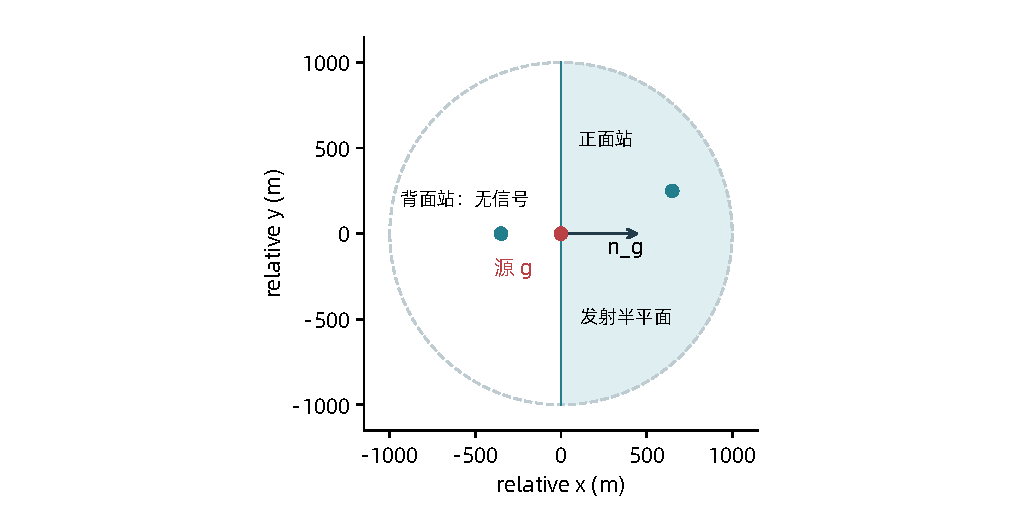
\includegraphics[width=0.68\linewidth]{figures/fig08_no_signal.pdf}
\caption{定向源的无信号反例。测站位于源的发射背面，即使距离小于1000 m也无法接收。无信号时保留位置区域，光学清除仍只受20 m距离条件限制。}
\end{figure}

\subsubsection{5.4.2 搜索站布设与连续覆盖}\label{ux641cux7d22ux7ad9ux5e03ux8bbeux4e0eux8fdeux7eedux8986ux76d6}

\textbf{（1）任意发射方向下的发现条件。} 设固定站集为\(\mathcal V\)，与未完成站编号集合\(\mathcal S_t\)区分。根据最小接收半径，要求对连续源域内任意位置\(g\)和任意发射方向单位向量\(n\)，均有

\[
\forall g\in\Omega,\ \forall n\in\mathbb S^1,
\ \exists s\in\mathcal V:
\|s-g\|<1000,\quad n^{\mathsf T}(s-g)\ge0.
\]

严格距离不等号用于构造接收裕量，发射半平面则按题设包含边界。该条件保证定向源能够被发现，也保证可见范围更大的全向源能够被发现。

\textbf{近距凸包引理。} 若对源位置\(g\)，存在一组测站\(W_g\subseteq\mathcal V\)满足

\[
g\in\operatorname{conv}(W_g),\qquad
\max_{w\in W_g}\|w-g\|<1000, \tag{12}
\]

则任意发射方向均至少可被一站接收。设\(g=\sum_i\lambda_iw_i\)，其中\(\lambda_i\ge0\)、\(\sum_i\lambda_i=1\)。若全部站均不可见，则\(n^{\mathsf T}(w_i-g)<0\)；加权求和得到

\[
0=n^{\mathsf T}\!\left(\sum_i\lambda_iw_i-g\right)
=\sum_i\lambda_i n^{\mathsf T}(w_i-g)<0,
\]

矛盾。因此至少一个近距站位于发射正面或边界。\(W_g\)仅用于证明，策略无须知道真实源的位置。

将目标域划分为三角网\(\mathcal T\)，若满足

\[
\Omega\subseteq\bigcup_{\tau\in\mathcal T}\tau,
\qquad
\max_{\tau\in\mathcal T}\max_{a,b\in V(\tau)}\|a-b\|<1000,
\]

则每个源所在三角形的三个顶点均可作为见证站。三角形内任一点到一个顶点的距离不超过最长边，故连续发现要求转化为三角网覆盖和有限边长核验。

\begin{figure}[!htbp]
\centering
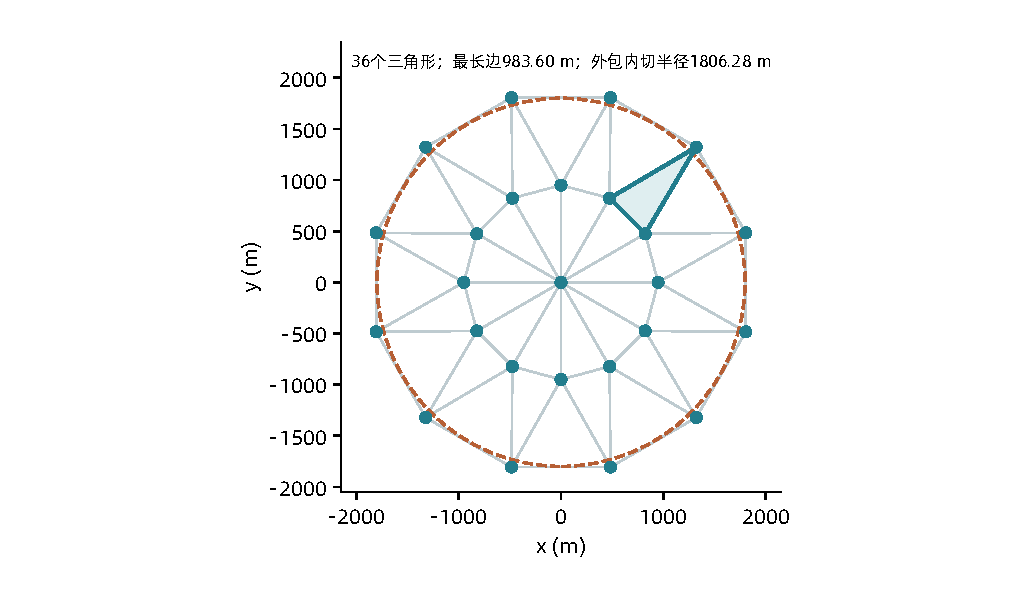
\includegraphics[width=0.78\linewidth]{figures/fig09_q4_cover.pdf}
\caption{25站双环搜索构造。中心站与内、外环分别位于0、950和1870 m处，两环错开15°，连接形成36个三角形。最长边小于1000 m，外环正多边形包围目标圆域，从而对任意源位置和发射方向提供发现保证。}
\end{figure}

\textbf{（2）双环构造。} 取中心站、内外两个正12边形环，半径分别为950、1870 m，错开15°：

\[
\begin{aligned}
s_0&=(0,0),\\
a_k&=950(\cos(k\pi/6),\sin(k\pi/6)),\\
b_k&=1870(\cos(k\pi/6+\pi/12),\sin(k\pi/6+\pi/12)),
\quad k=0,\ldots,11.
\end{aligned} \tag{13}
\]

下标按模12连接\((s_0,a_k,a_{k+1})\)、\((a_k,a_{k+1},b_k)\)和\((a_k,b_{k-1},b_k)\)，得到36个三角形。最长边983.60 m小于1000 m，外环内切半径\(1870\cos15^\circ=1806.28\) m大于1800 m，因此三角网覆盖源域并满足近距凸包条件。图13分别示意局部可见性和全局包围。

对等站数正双环构造，外环须满足\(r_o\cos(\pi/m)\ge1800\)及\(2r_o\sin(\pi/m)<1000\)，推出每环至少12站。该下界只适用于此构造族，25站不是一般布局的最少站数证明；半径选择与边长核验见附录E.4。

\begin{figure}[!htbp]
\centering
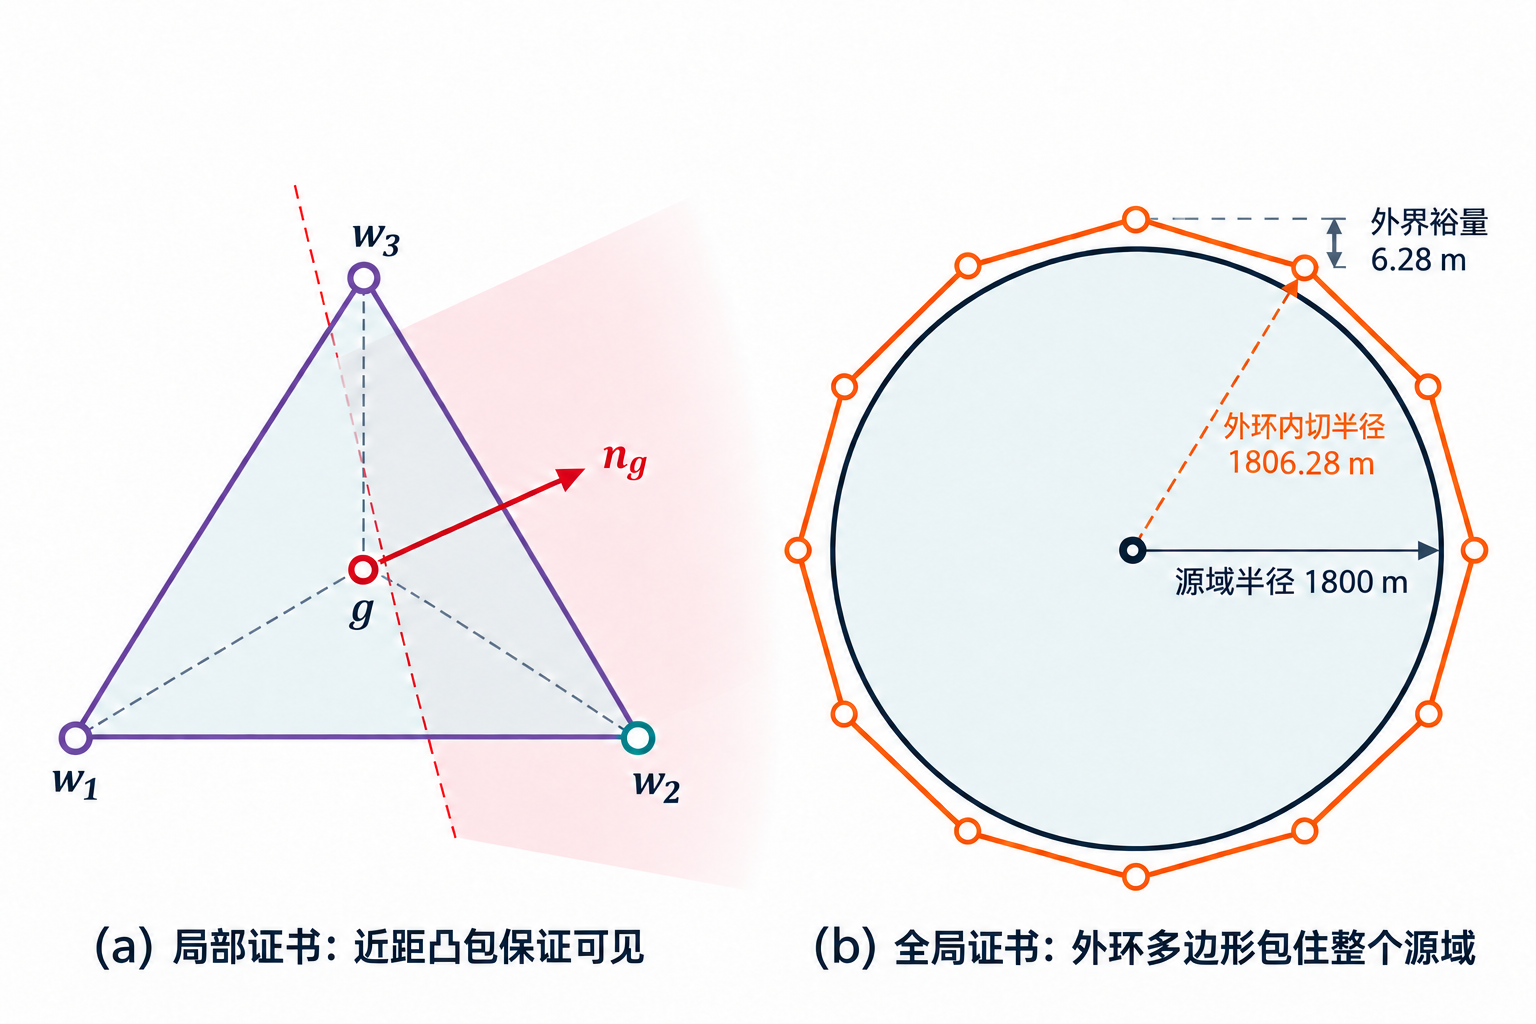
\includegraphics[width=0.76\linewidth,trim={0 25bp 0 170bp},clip]{figures/fig20_q4_coverage_certificate.png}
\caption{定向源发现保证的局部与全局几何示意。（a）源位于近距站的凸包内，任意发射方向至少有一个站可见；（b）外环正十二边形包围半径1800 m的源域，内切半径为1806.28 m。图不按比例绘制；内切半径指圆心到边的垂距，顶点到圆心的外环半径为1870 m。}
\end{figure}

\FloatBarrier
\subsubsection{5.4.3 交会定位与光学清除}\label{ux4ea4ux4f1aux5b9aux4f4dux4e0eux5149ux5b66ux6e05ux9664}

\textbf{（1）局部中心与补测。} 设位置区域\(P_c\)的顶点为\(x_1,\ldots,x_v\)，取最长顶点对的中点及其覆盖半径：

\[
(i^*,j^*)\in\arg\max_{i,j}\|x_i-x_j\|,
\qquad m_c=\frac{x_{i^*}+x_{j^*}}2,
\qquad\rho_c=\max_i\|x_i-m_c\|.
\]

若\(\rho_c<20\) m，前往\(m_c\)即可保证清除；程序使用\(\rho_c<20-10^{-5}\) m以保留余量。此处对全部顶点核验覆盖，不能将半径直接取为\(D(P_c)/2\)。

若尚未满足清除条件且正常方位不足两条，沿首测横向构造

\[
q_c^{\pm}=m_c\pm300v_c.
\]

先访问距离当前位置较近的一侧，若无信号再访问另一侧；一旦取得第二条正常方位，即停止补测、更新\(P_c\)并重新计算\(m_c,\rho_c\)。近场反馈直接在测点清除。300 m为固定启发式偏移，不承担再次接收保证。两侧均无信号，或已有至少两条正常方位仍不足以直接清除时，进入有限光学覆盖。

\textbf{（2）光学网格及有限清除。} 沿首测基\(u_c,v_c\)取\(P_c\)的外包矩形，投影端点为\(\ell_e=\min_{x\in P_c}e^{\mathsf T}x\)、\(h_e=\max_{x\in P_c}e^{\mathsf T}x\)。各方向划分为\(n_e=\max(1,\lceil(h_e-\ell_e)/28\rceil)\)等份，使格边\(d_u,d_v\le28\) m；从近端开始按蛇形访问格心，成功即停止（图14）。格心公式见附录E.5。

\[
\max_{x\text{ 在格内}}\|x-p_{ij}\|
\le\tfrac12\sqrt{d_u^2+d_v^2}
\le14\sqrt2\approx19.80<20\ \mathrm m.
\]

真源始终在区域内，故必有一格覆盖它，且光学清除不受方向限制。初始矩形至多为\(1500\times52.62\) m，网格上界为\(\lceil1500/28\rceil\lceil52.62/28\rceil=108\)格；有效测向可缩小范围。该数为初始访问上界，实际可提前清除，失败尝试的移动与3 s光学费用均计入总时间。

\begin{figure}[!htbp]
\centering
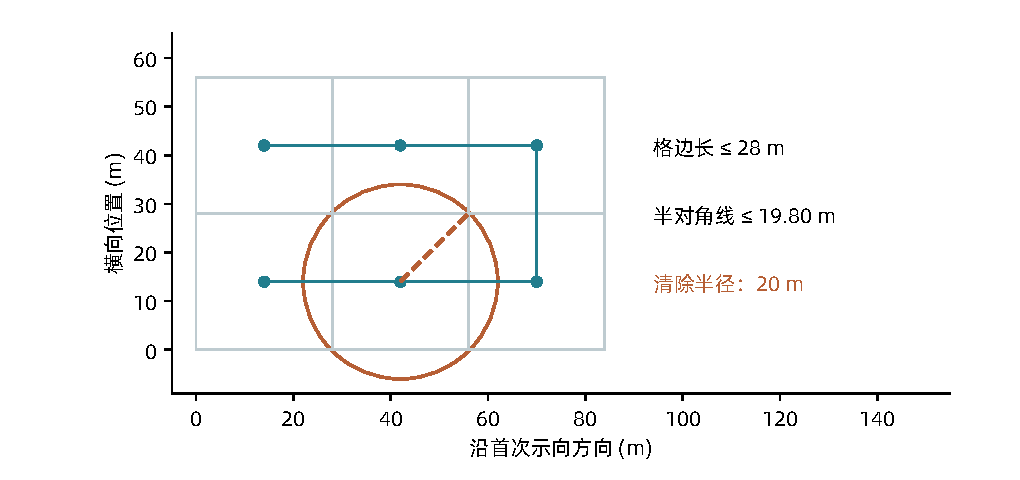
\includegraphics[width=0.82\linewidth]{figures/fig10_optical.pdf}
\caption{有限光学网格。每格两边不超过28 m，因此格心的20 m清除圆覆盖整个格。图示六格局部区域及蛇形访问顺序，实际格数由当前位置区域决定，清除成功后停止访问。}
\end{figure}

\subsubsection{5.4.4 搜索与清除的滚动调度}\label{ux641cux7d22ux4e0eux6e05ux9664ux7684ux6edaux52a8ux8c03ux5ea6}

\textbf{（1）任务代表点与访问顺序。} 沿用5.3.3的搜索---源服务任务集合及开放路径目标\(L_t(\pi)\)。搜索任务的代表点为固定站坐标，源任务的代表点改用位置区域的面积重心

\[
z_c=\frac{1}{\operatorname{area}(P_c)}\int_{P_c}x\,\mathrm dx;
\]

面积退化时取\(m_c\)。\(z_c\)只用于估计任务之间的路程；执行源服务时，补测和清除仍按上一节的\(m_c\)及覆盖判据确定，不要求先访问\(z_c\)。

从当前位置出发，以最近邻规则生成一条开放路线，再作至多50轮2-opt调整，每轮选择使路径缩短最多的片段反转；无进一步缩短时提前结束。仅执行所得路线的首项完整任务，完成整站扫描或该源清除后再更新并排序。该规则近似优化代表点间的行程，未完整计入源服务内部移动、检测费用和提前发现第16源的价值，其整局效果由6.3节评价。

\textbf{（2）必要频道与观测筛选。} 对尚未完成的搜索站，所有未知频道均需检测；已清除频道不再检测。对于已知未清频道\(c\)，若\(\rho_c\)已满足直接清除阈值，保留其清除任务而跳过本站测向。否则，以\(p\)指向\(m_c\)的方位为参考，将\(P_c\)各顶点相对于\(p\)的方位差归一到\([-\pi,\pi)\)，用其最大值与最小值之差定义顶点方位跨度\(\omega_c(p)\)。

以20 m为理想清除阈值，本站需测频道可写为

\[
\begin{aligned}
\mathcal Q_t(p)={}&\bigl(\{1,\ldots,20\}\setminus\mathcal D_t\bigr)\\
&\cup\{c\in\mathcal D_t\setminus\mathcal C_t:
\rho_c\ge20,\ \omega_c(p)\ge3^\circ\}.
\end{aligned}
\]

程序在清除阈值中采用前述数值余量，并优先检测当前频道，其余按编号顺序进行。正常方位更新相应区域，近场反馈可当场清除；无信号仅保存记录。3°规则用于减少低信息量检测，被跳过的已知源始终保留为源服务任务。第四问在搜索站利用这些观测更新多个频道的区域，局部补测则只服务当前目标。

\subsubsection{5.4.5 完整算法与求解结果}\label{ux5b8cux6574ux7b97ux6cd5ux4e0eux6c42ux89e3ux7ed3ux679c}

\textbf{（1）停止条件与算法流程。} 将25个固定站编号为0---24，记\(\mathcal N_c\)为仍未知频道\(c\)取得无信号反馈的站编号集合。任务完成条件为

\[
\begin{aligned}
&|\mathcal C_t|=16,\\
&\text{或}\quad \mathcal C_t=\mathcal D_t,\qquad
\mathcal N_c=\{0,\ldots,24\}\quad
\forall c\in\{1,\ldots,20\}\setminus\mathcal D_t.
\end{aligned}
\]

前者利用源数上限，后者同时核验已知源清除与未知频道排除。单个无信号反馈不足以删除附近圆盘，但一个未知频道在具有连续发现保证的全部站点均无信号，则可排除该频道源存在。

算法循环如下：

\begin{enumerate}
\def\labelenumi{\arabic{enumi}.}
\tightlist
\item
  从原点建立25站任务及空的观测、发现和清除记录。
\item
  检查停止条件；否则按5.4.4排序并执行首项完整任务。已发现16频道时取消未知搜索。
\item
  搜索任务扫描必要频道，源服务依次检查直接清除、两侧补测及光学网格；依据反馈更新记录后回到步骤2。数量达到16时，在整站结束后的下一轮规划中取消搜索。
\item
  区域为空、保证清除失败、网格耗尽或接口异常、超时，均报未完成，不能以任务池为空替代停止核验。
\end{enumerate}

连续覆盖保证发现，区域保真与有限光学覆盖保证清除。外层至多完成25项搜索和16项源服务，路线调整与格心访问也有限；完成保证依赖题面模型、合法反馈与准确几何，实际执行还受数值与时限约束。

算法输出任务访问序列、频道清除记录、时间分解及停止依据。构造核验表见附录E.4，模块接口见附录A.3；25站布局、重心排序与观测筛选共同构成推荐方案，其整体收益由6.3节评价，正式结果见6.4节。

\section{6 模型分析与评价}\label{ux6a21ux578bux5206ux6790ux4e0eux8bc4ux4ef7}

本章结合自建配对实验、正式测试记录和几何证明，从任务完成情况、耗时表现及适用条件三个方面评价模型。

\subsection{6.1 实验设计与评价方法}\label{ux5b9eux9a8cux8bbeux8ba1ux4e0eux8bc4ux4ef7ux65b9ux6cd5}

\textbf{实验与独立单位。} 性能比较来自冻结的自建完整流程记录，同布局、同误差条件下配对；生成器不代表官方源分布。候选在开发后冻结源码、配置及规则，再生成新布局验证。Q3冻结基线为历史第十九轮组合；Q4历史比较以31站初始方案为基线，动态比较以成熟25站方案为基线，两个阶段的改善不能相加。

\begin{table}[H]
\centering\small
\caption{自建实验组、独立布局与用途}
\begin{tabular}{@{}>{\raggedright\arraybackslash}p{\dimexpr 0.180\linewidth-1.5000\tabcolsep\relax}>{\raggedright\arraybackslash}p{\dimexpr 0.160\linewidth-1.5000\tabcolsep\relax}>{\raggedright\arraybackslash}p{\dimexpr 0.360\linewidth-1.5000\tabcolsep\relax}>{\raggedright\arraybackslash}p{\dimexpr 0.300\linewidth-1.5000\tabcolsep\relax}@{}}
\toprule
证据组 & 独立布局 & 每布局条件 & 用途\tabularnewline
\midrule
Q2候选复核 & 不适用 & 36,421个几何场景/候选 & 采样定位直径\tabularnewline
Q3最终验证 & 120 & 4误差场×2舍入环境 & 联合方案与消融\tabularnewline
Q4历史验证 & 96+96，互不重叠 & 1误差场；两批各1种环境 & 31站、25站及删减对照\tabularnewline
Q4动态验证 & 120 & 4误差场×2舍入环境 & 25站与4个候选\tabularnewline
\bottomrule
\end{tabular}
\end{table}

\textbf{统计口径。} 主要效应为\(100(1-\overline T_{\rm candidate}/\overline T_{\rm base})\)，正值为省时；图16、20以时间变化表示，负值为省时。均值、分位数及极值按运行等权计算，区间以独立布局为重采样块，保留块内条件：Q3按6类分层重采样20,000次；Q4历史两批各10,000次，动态验证按6类分层10,000次\textsuperscript{\cite{efron1979}}。条件重放不增加独立样本数，区间只反映自建生成器下的采样不确定性。分位数、图形口径与布局类别见附录E.6。

\textbf{选择与核验。} 后续候选事先要求完整率不降、平均降时至少5\%、P95不恶化；最终验证不再调参。失败及超时预设计入\(\max(T,360000)\) s，本批未触发，慢例全部保留。实现检查覆盖退化几何、响应重放、清除计数与停止条件，并以通用求解器交叉复核Q2；规模见附录B.6，检查不替代形式证明。正式测试另见6.4节，补充开发不并入原验证。

\FloatBarrier
\subsection{6.2 问题三：实验结果与机制分析}\label{ux95eeux9898ux4e09ux5b9eux9a8cux7ed3ux679cux4e0eux673aux5236ux5206ux6790}

\subsubsection{6.2.1 Q3的试错：集合变紧并不会自动省时}\label{q3ux7684ux8bd5ux9519ux96c6ux5408ux53d8ux7d27ux5e76ux4e0dux4f1aux81eaux52a8ux7701ux65f6}

开发中，单纯沿集合中心逼近比冻结基线慢11.44\%，加入视差和共享仍无平均优势；共同排序后组合才降时12.83\%。单方位光学覆盖、接收边界测距均增加耗时，共享还须逐频道检查接收条件。这说明局部定位改进需与任务顺序联合评价；开发及单例诊断见附录B.4。

\subsubsection{6.2.2 Q3的锁定验证：平均更快，但保留少量明显慢例}\label{q3ux7684ux9501ux5b9aux9a8cux8bc1ux5e73ux5747ux66f4ux5febux4f46ux4fddux7559ux5c11ux91cfux660eux663eux6162ux4f8b}

120个新布局、两种环境中，联合方案均完成全部运行。主模型平均省时10.27\%，95\%区间{[}9.14\%,11.35\%{]}；舍入压力下省时10.07\%，区间{[}8.95\%,11.15\%{]}。各行含同一120布局的4次条件运行，共480次；完整耗时如下。

\begin{table}[H]
\centering\small
\caption{Q3锁定验证的完整流程结果}
\begin{tabular}{@{}llrrrrr@{}}
\toprule\noalign{}
误差环境 & 方案 & 均值/s & 中位数/s & P95/s & 本批最大/s & 完成局数 \\
\midrule\noalign{}

有界读数 & 冻结基线 & 3323.52 & 3631.26 & 4517.29 & 5111.40 & 480/480 \\
有界读数 & 联合方案 & 2982.18 & 3234.21 & 3823.72 & 4217.81 & 480/480 \\
舍入压力 & 冻结基线 & 3319.49 & 3616.01 & 4505.79 & 5086.03 & 480/480 \\
舍入压力 & 联合方案 & 2985.19 & 3234.30 & 3827.73 & 4217.91 & 480/480 \\
\bottomrule
\end{tabular}
\end{table}

图15概括总时间分布，图16保留六类布局的全部配对结果；平均改善并不意味着逐例占优。

\begin{figure}[!htbp]
\centering
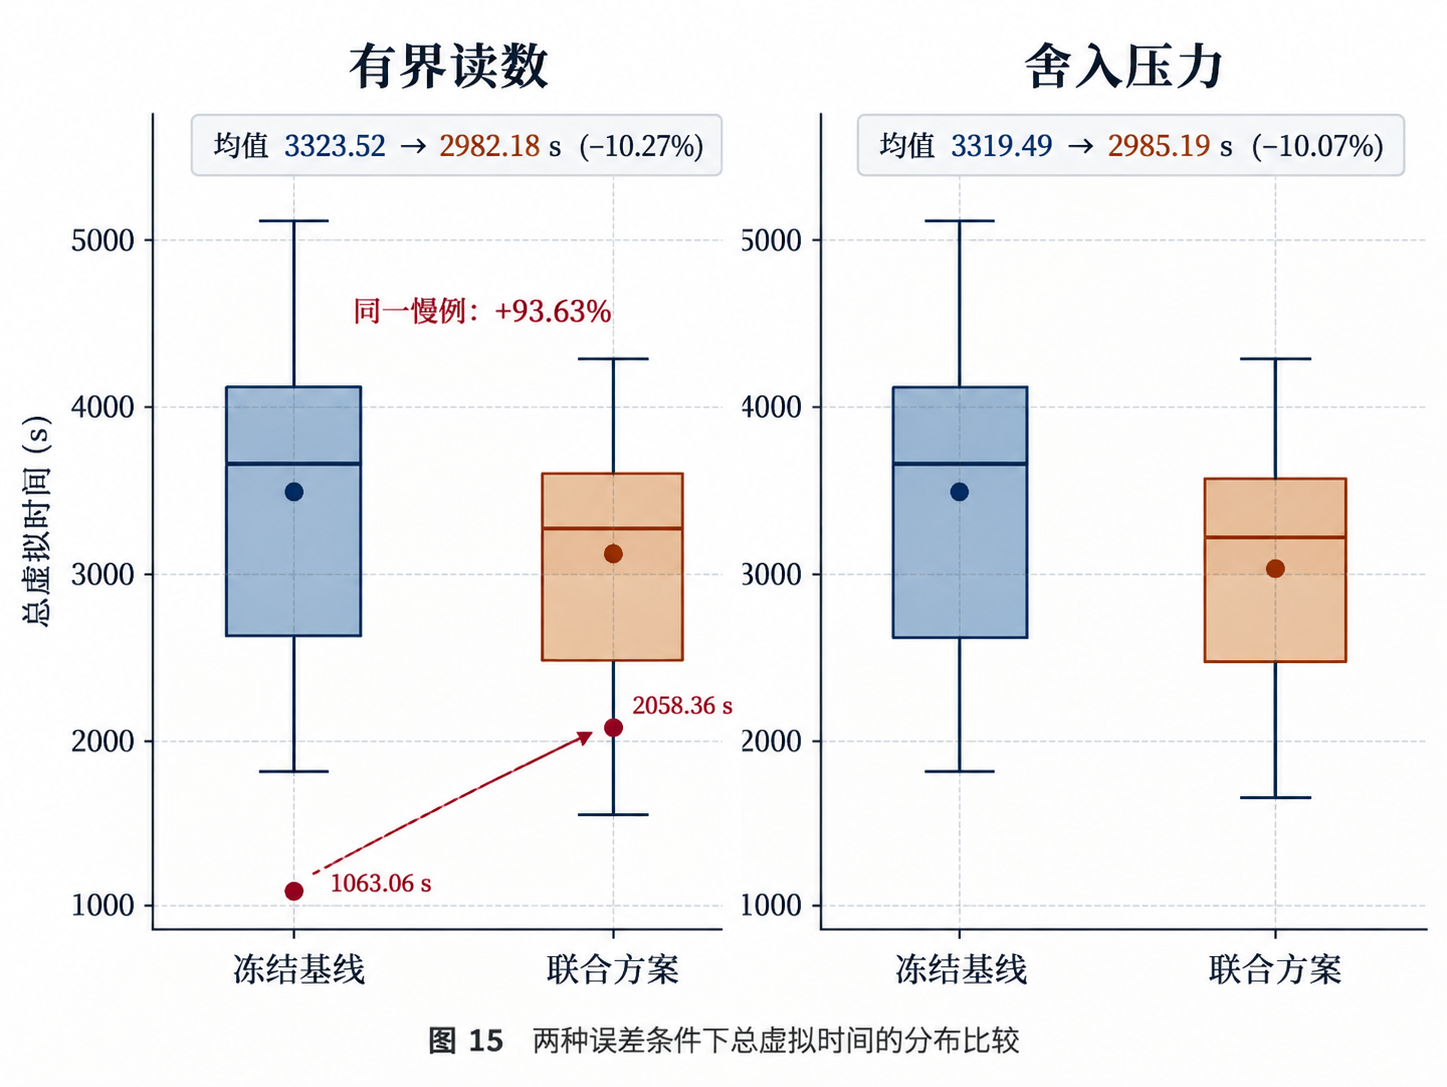
\includegraphics[width=0.80\linewidth,trim={0 95bp 0 0},clip]{figures/fig19_q3_time_distribution_optimized.png}
\caption{Q3两种误差环境的总时间分布比较示意。每组480次运行，对应120个独立布局；左图红线标出同一慢例从1063.06 s增至2058.36 s，退化93.63\%。图中部分统计点位为示意，精确均值和分位数以正文表格及源数据为准；箱体不表示效应置信区间。}
\end{figure}

\begin{figure}[!htbp]
\centering
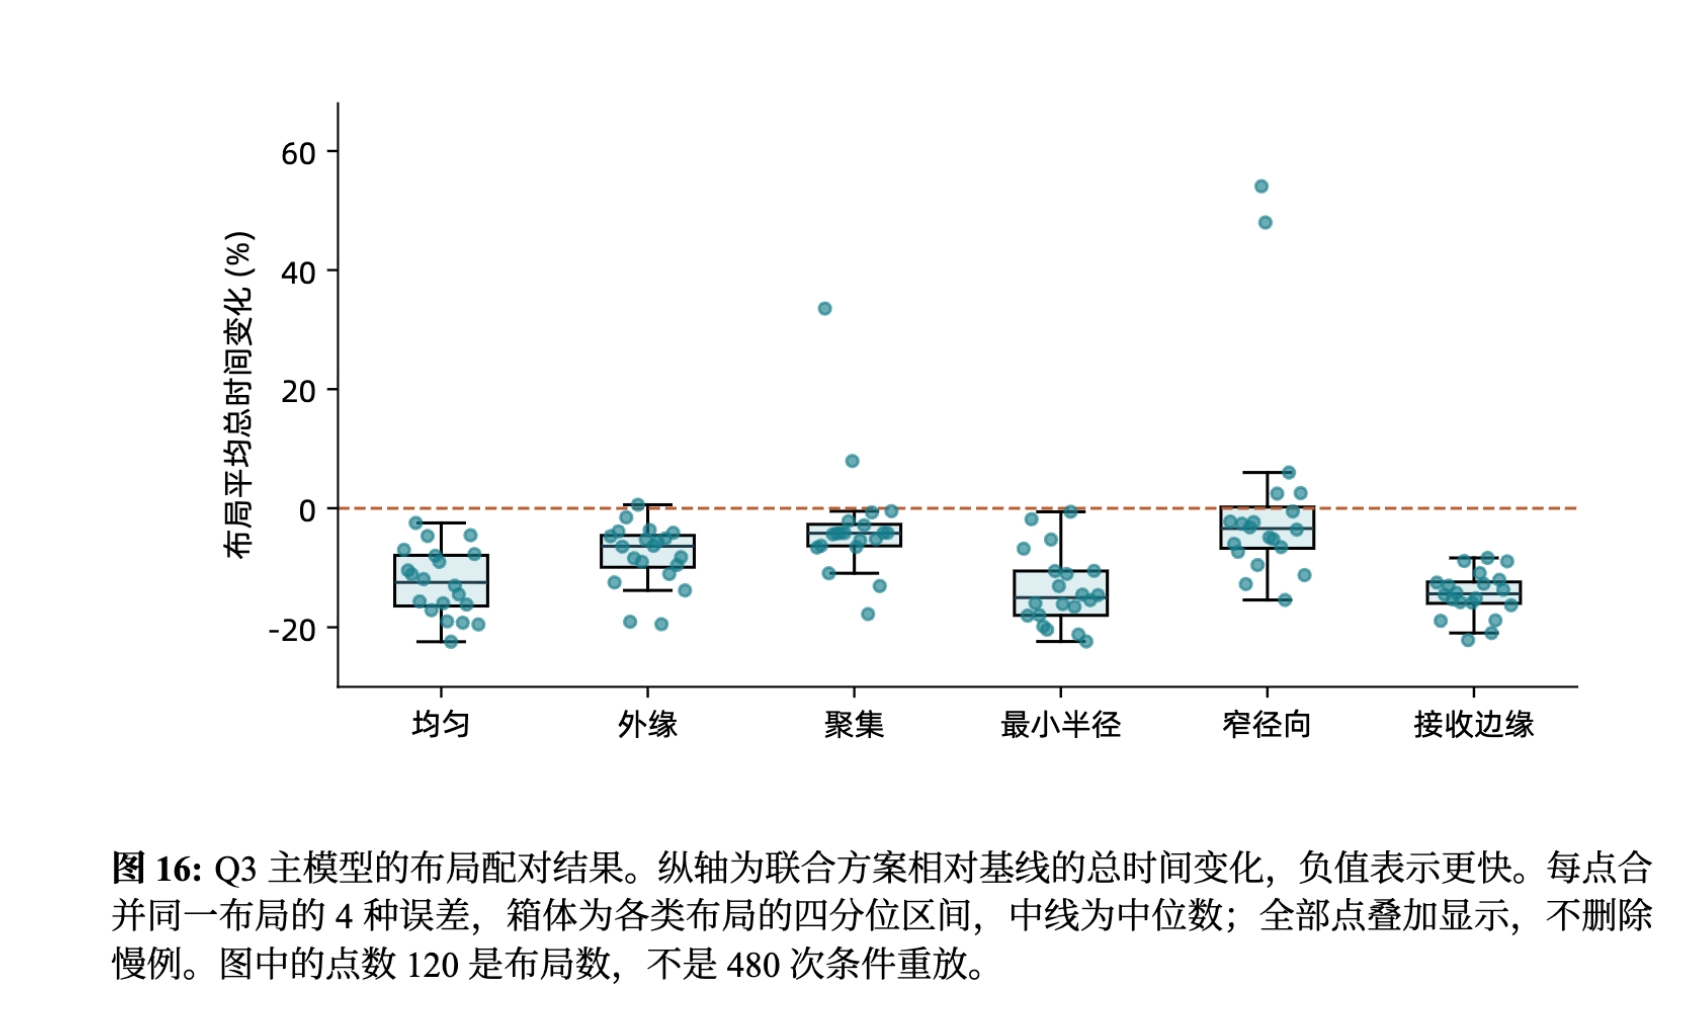
\includegraphics[width=0.90\linewidth,trim={190bp 240bp 80bp 80bp},clip]{figures/fig11_q3_distribution_optimized.jpg}
\caption{Q3主模型的布局配对结果。纵轴为联合方案相对基线的总时间变化，负值表示更快。每点合并同一布局的4种误差，箱体为各类布局的四分位区间，中线为中位数；全部点叠加显示，不删除慢例。图中的点数120是布局数，不是480次条件重放。}
\end{figure}

主模型435次更快、45次更慢，舍入压力下433次更快、47次更慢。最差为16源聚集布局：基线1063.06 s、联合方案2058.36 s，慢93.63\%。原点可接收15源，联合方案却在发现最后一源前访问更多站，增加791.31 s移动、185 s检测与37 s切频。该例揭示距离排序可能错失第16源带来的提前停止机会；逐动作诊断见附录E.7，图16按布局合并后最高点不等于单次退化93.63\%。

\FloatBarrier
\subsubsection{6.2.3 Q3为何更快：省下的移动支付了额外观测}\label{q3ux4e3aux4f55ux66f4ux5febux7701ux4e0bux7684ux79fbux52a8ux652fux4ed8ux4e86ux989dux5916ux89c2ux6d4b}

图17按实际动作分解净收益：每局移动省383.25 s，检测及切频多用63.76、8.14 s，光学省29.98 s，清除附加费用不变，净省341.33 s。额外观测换来了更少行走。

\begin{figure}[!htbp]
\centering
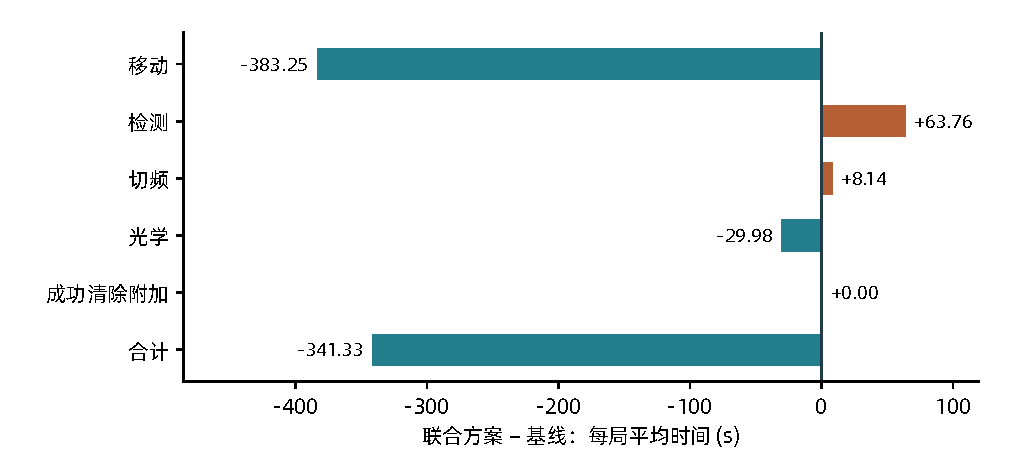
\includegraphics[width=0.88\linewidth]{figures/fig12_q3_cost.pdf}
\caption{Q3主模型的动作代价分解。数值为联合方案减去基线的每局平均时间，负值为节省。合计是前五项之和；不能再叠加搜索、定位等阶段耗时，否则会重复计费。}
\end{figure}

联合方案960次运行无失败光学尝试、无网格回退；回退仍保留为有限清除保障。主模型逐局每源平均时间由269.71降至242.21 s，舍入压力下由269.36降至242.38 s。

图18以共同父方案逐项消融：删除目标原地再观测省25.00 s；删除首次视差、完整行程规划或信息门控分别慢243.72、37.20、27.00 s。``删除门控''仍共享观测，仅取消收缩价值筛选。各差值不可相加，父方案也不等于历史冻结基线；完整开关矩阵及P95见附录E.8。

\begin{figure}[!htbp]
\centering
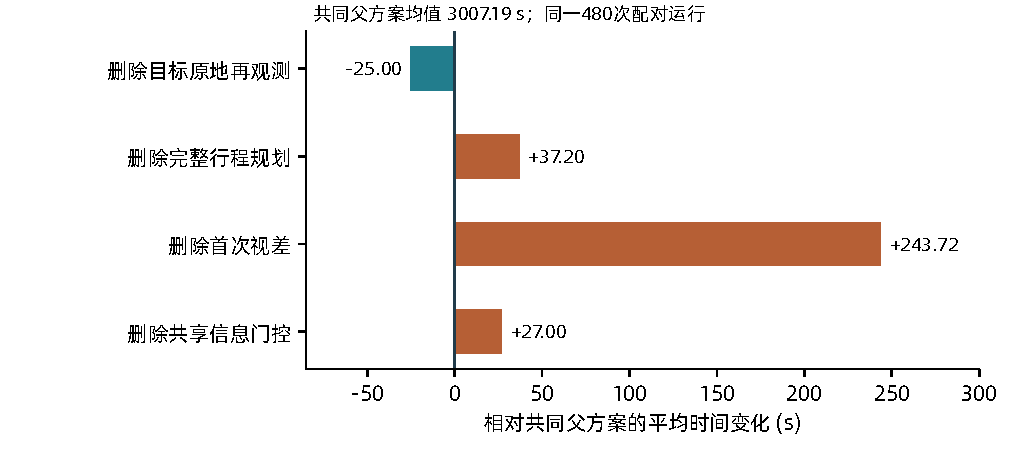
\includegraphics[width=0.88\linewidth]{figures/fig13_q3_ablation.pdf}
\caption{Q3最终主模型的共同父方案消融。每行是在同一父方案上删除一项机制后的均值变化，使用同一480次配对运行；负值支持删除，正值支持保留。图为配对差的描述性均值，不单独宣称各行统计显著。}
\end{figure}

\FloatBarrier
\subsection{6.3 问题四：实验结果与方案比较}\label{ux95eeux9898ux56dbux5b9eux9a8cux7ed3ux679cux4e0eux65b9ux6848ux6bd4ux8f83}

\subsubsection{6.3.1 Q4为何保留25站：覆盖成立只是第一道门槛}\label{q4ux4e3aux4f55ux4fddux755925ux7ad9ux8986ux76d6ux6210ux7acbux53eaux662fux7b2cux4e00ux9053ux95e8ux69db}

开发中的具体21站构造在25 m粗网格上无漏点，细化后却出现近站最大方向空隙182.68°，可漏掉180°定向发射，说明粗采样不能替代连续证明。22站构造虽通过连续证书，同批验证仍比25站慢5.24\%、3.39\%；站数少不保证实际扫描少，案例见附录E.9。

图19比较31站初始基线与25站完整方案。两批各96个独立布局，25站平均时间为6640.86、6694.69 s，分别省41.83\%、41.24\%，配对95\%区间为{[}40.35\%,43.24\%{]}、{[}39.70\%,42.79\%{]}。各批96次均更快，所有比较方案均完整清除。

\begin{figure}[!htbp]
\centering
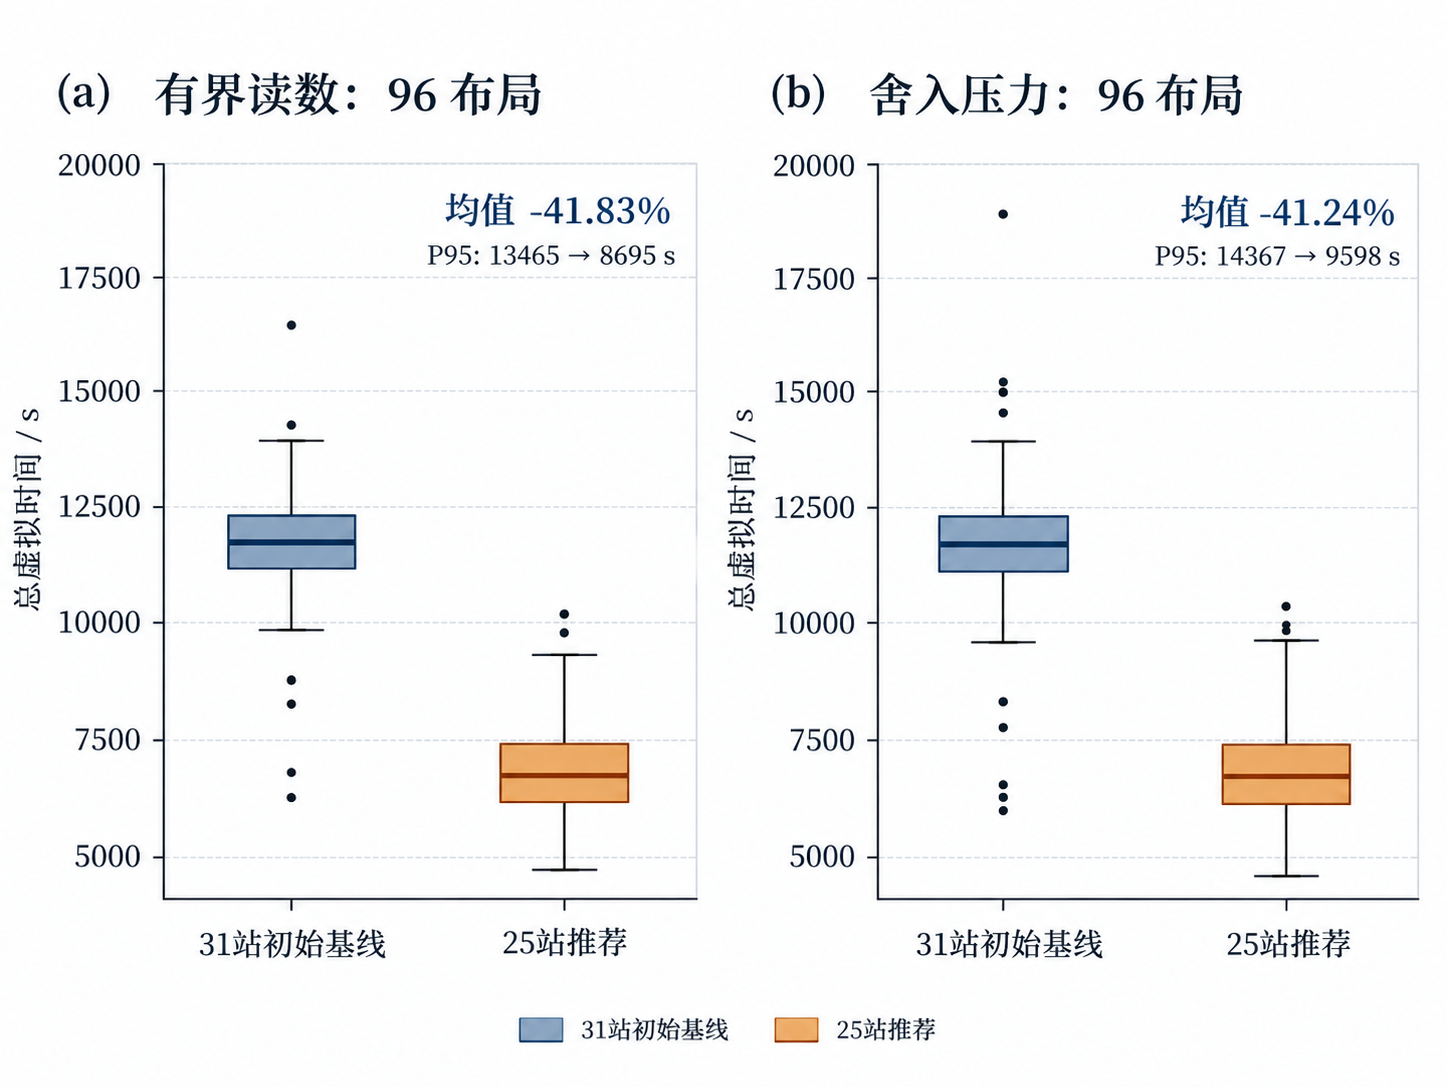
\includegraphics[width=0.80\linewidth]{figures/fig14_q4_historical_optimized.png}
\caption{Q4两批历史自建验证的时间分布比较示意。两批各96个互不重叠布局，每批内部31站与25站方案配对；图中标注均值降时及P95变化。箱体和点位仅概括分布形态，精确中位数、分位数和极值以正文及源数据为准；箱体不表示均值置信区间。}
\end{figure}

25站的P95为8694.62、9598.33 s，低于基线13465.02、14367.42 s；删除重心排序后两批均慢超过11\%，删除低信息量观测筛选后慢约4.6\%。因此约41\%收益属于布局、排序和观测筛选的整体，不能全归于减少6站。中位数、极值与代价细分见附录E.9。

\FloatBarrier
\subsubsection{6.3.2 Q4后续试错：动态覆盖安全，却没有足够的整局收益}\label{q4ux540eux7eedux8bd5ux9519ux52a8ux6001ux8986ux76d6ux5b89ux5168ux5374ux6ca1ux6709ux8db3ux591fux7684ux6574ux5c40ux6536ux76ca}

进一步尝试以已到达位置替站，或移动内环站缩短局部路线；每次修改须独立重建三角网并通过连续覆盖核验，预算不足则保留原站。组合开发省时2.33\%，未达5\%门槛，随后在新布局上锁定验证。

五方案共4800次运行全部清除；每方案为同一120布局×8条件。动态组合平均6719.67 s，相对25站的6744.38 s省0.366\%，95\%区间{[}−0.183\%,0.921\%{]}跨零，P95仅降0.394\%（图20）。组合706次更快、254次更慢；移动省37.00 s，但额外检测、光学及切频抵消部分收益，净省24.71 s。五方案完整统计见附录E.10。

\begin{figure}[!htbp]
\centering
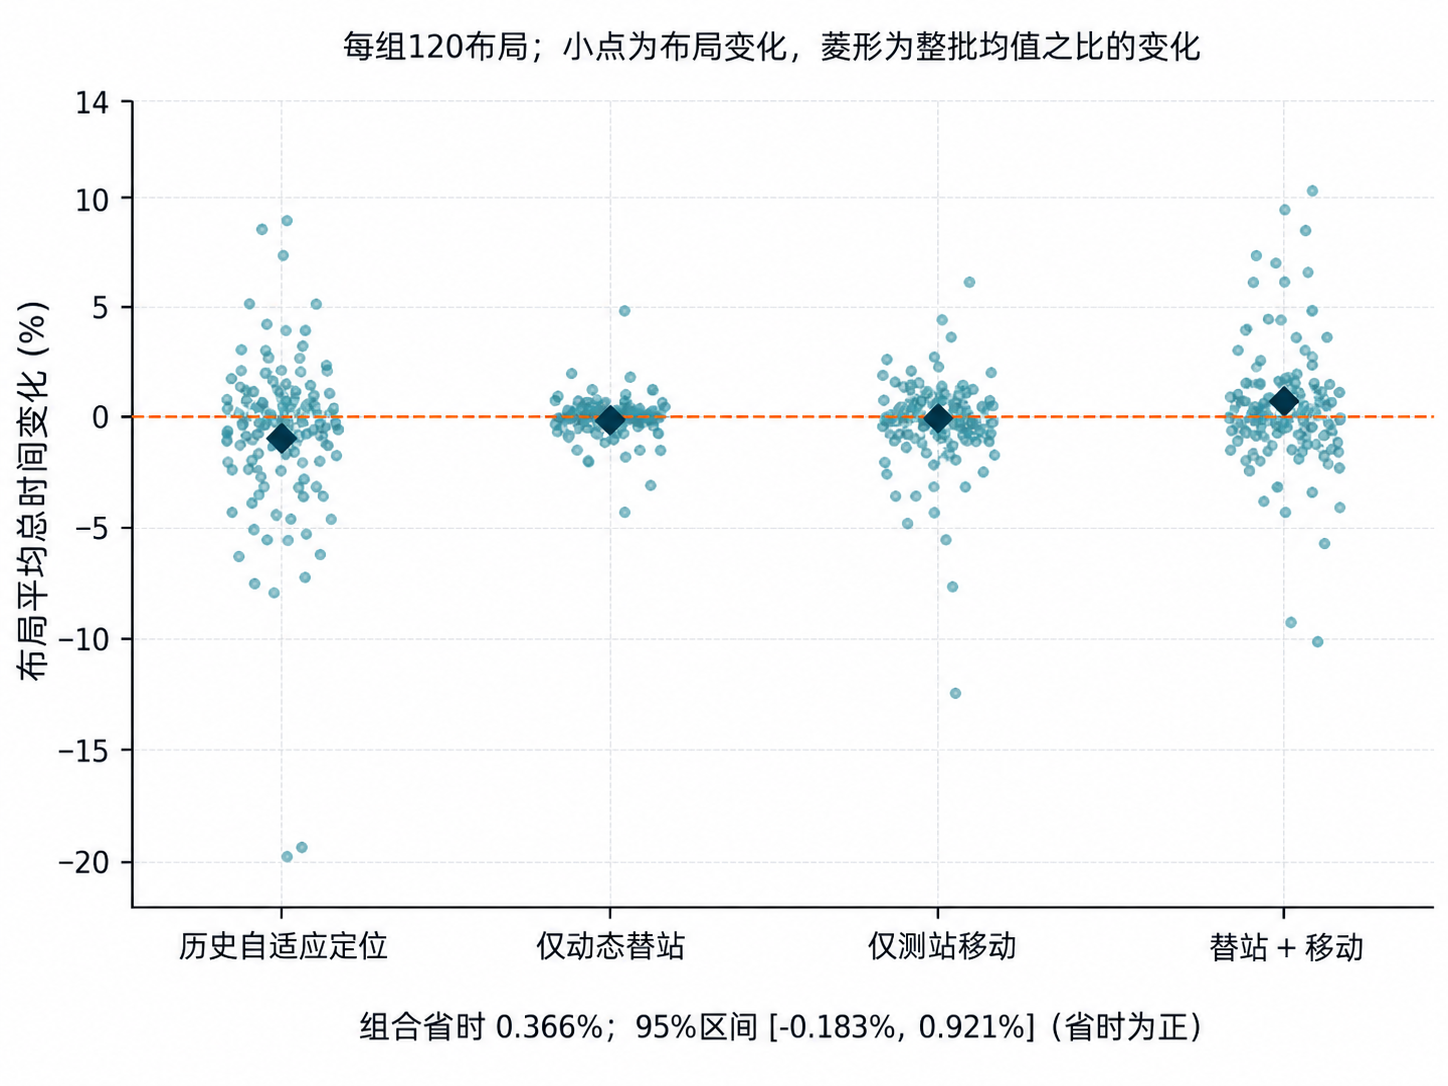
\includegraphics[width=0.80\linewidth]{figures/fig15_q4_latest_optimized.png}
\caption{Q4最新锁定验证的布局配对分布示意。每组对应120个布局，每个布局合并8种误差与舍入条件；纵轴为总时间变化，正值表示变慢，下方以省时为正报告效应区间。图中部分点位与核验统计存在偏差，组合菱形应对应时间变化−0.366\%，而非正值；精确配对结果以正文及源数据为准。}
\end{figure}

最差单例慢33.69\%：移动首个内环站103.88 m，局部预测路程缩短42.06 m，实际扫描却从7站增至19站，第16源发现推迟2717.83 s。该例未发生动态替站，不能归因于该操作。逐动作记录支持发现顺序变化的解释，但无反事实实验分配单步因果损失。历史自适应定位虽省1.931\%，仍未达5\%门槛且最大值更高。因此保留原25站推荐，动态覆盖仅作为可行但收益不足的扩展。

\FloatBarrier
\subsection{6.4 正式测试结果}\label{ux6b63ux5f0fux6d4bux8bd5ux7ed3ux679c}

2026年9月13日，两问各完成三次正式测试。案例编码来自正式行为日志，清除数逐条核验成功响应；平均定位清除时间为退出时总虚拟时间除以成功清除数。原名日志与版本对应见附录C。

\Needspace{8\baselineskip}
\textbf{第三问正式测试结果}

\begingroup\small
\begin{longtable}[]{@{}lrrr@{}}
\toprule
测试案例编码 & 清除干扰源个数 & 平均定位清除时间/s & 程序运行时间/s\tabularnewline
\midrule
\endhead
5ER6-BK3Y-KHDQ-MUQT & 10 & 295.56 & 0.434\tabularnewline
VUK9-G6FH-ACSC-KFYG & 16 & 243.03 & 0.682\tabularnewline
3BEW-YK5X-AE2M-SJND & 12 & 254.64 & 0.588\tabularnewline
\bottomrule
\end{longtable}
\endgroup

\Needspace{8\baselineskip}
\textbf{第四问正式测试结果}

\begingroup\small
\begin{longtable}[]{@{}lrrr@{}}
\toprule
测试案例编码 & 清除干扰源个数 & 平均定位清除时间/s & 程序运行时间/s\tabularnewline
\midrule
\endhead
JHQ9-ZVTT-CGAR-GVTX & 10 & 575.57 & 1.182\tabularnewline
SXAN-9UWV-2X8Z-GZ58 & 15 & 388.30 & 1.691\tabularnewline
CEBG-3EHE-MGUQ-H96W & 11 & 578.52 & 1.146\tabularnewline
\bottomrule
\end{longtable}
\endgroup

程序运行时间为模拟器入场至主动退出的实时时间戳之差，与虚拟动作耗时分开。两问累计清除38、36源，三次每源平均时间的算术平均为264.41、514.13 s，六次均满足停止判据并主动退出。Q3无失败光学尝试，Q4第二、三次有5、6次未命中，费用已计入。逐次总时间见附录E.11。

Q3配置及策略哈希对应联合方案；Q4配置与25站布设对应推荐，未保存运行代码哈希，版本关联限于附录C。客户端未获源总数，故不另算官方清除率。每问仅3例且无同案例基线，正式结果支持实际可运行性，不能用于推断自建实验约10\%和41\%的相对降时。

\textbf{过程证据。} 图21上排来自Q4历史自建对照，首次全发现所需扫描站数中位数由20、20.5降至15、18；这是读取真值后的事后指标，不替代停止核验。中排为Q3正式38源：31源满足覆盖圆判据，7源由近场反馈清除。下排的相邻清除点间耗时含搜索、定位、移动与光学动作；清除终点与退出时刻不同，后续核验时间见附录E.11。

\begin{figure}[!htbp]
\centering
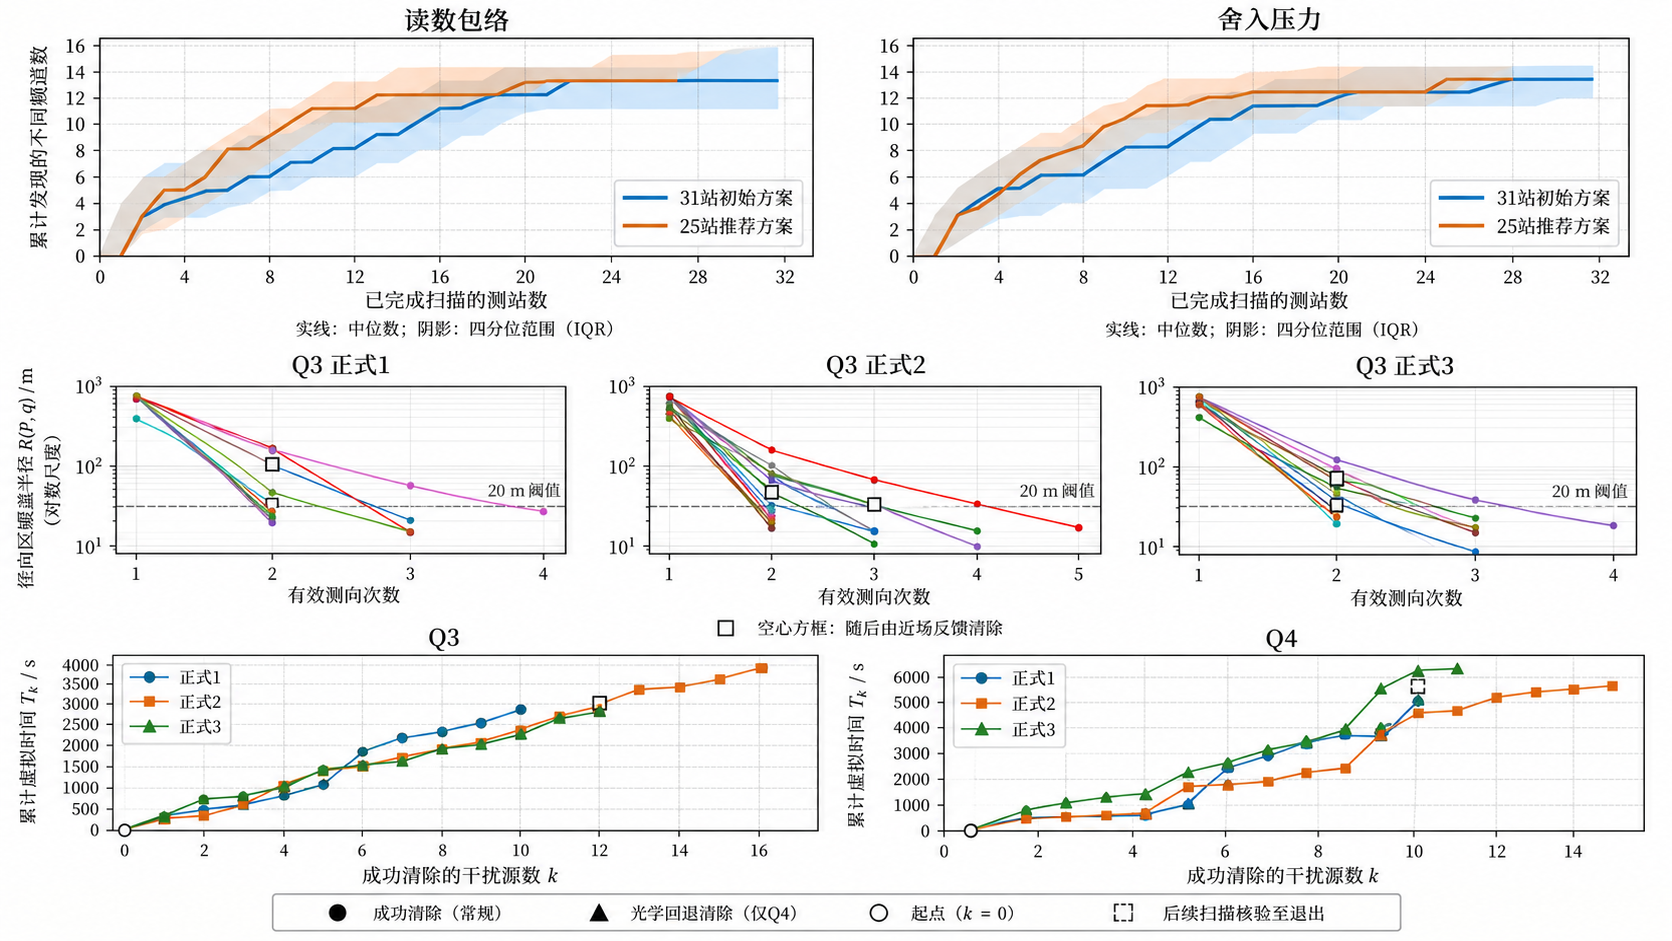
\includegraphics[width=0.98\linewidth]{figures/fig21_discovery_localization_clearance.png}
\caption{发现、定位与清除过程的示意汇总。上排为Q4两批历史自建对照，每批96个配对布局；实线表示中位数，阴影表示四分位范围，端值延伸不代表继续扫描，25站方案的实际预算仍为25站。中排为Q3三次正式测试的区域收敛，空心方框表示随后通过近场反馈清除。下排为两问各三次正式测试的清除与耗时关系，三角形表示光学回退清除。原图的阈值线位置及部分点位与核验记录有偏差，故仅用于过程示意；20 m判据、清除终点和退出时间以正文及源数据为准。}
\end{figure}

\FloatBarrier
\subsection{6.5 模型优点与理论保证}\label{ux6a21ux578bux4f18ux70b9ux4e0eux7406ux8bbaux4fddux8bc1}

位置集合将有界误差、接收和清除条件统一为可计算约束；七站覆盖与近距三角网分别提供全向、定向发现保证，有限光学网格补足失联后的清除。任务排序与观测共享在这些条件内改善效率。几何结论、按规则执行的条件性完成保证、配对实验的平均收益分属不同层次，不能相互替代。

\subsection{6.6 模型局限与适用边界}\label{ux6a21ux578bux5c40ux9650ux4e0eux9002ux7528ux8fb9ux754c}

证明依赖静态源、有界误差、半径下界及半平面发射；移动、遮挡或更窄发射扇区需重建覆盖。浮点外包与余量未经完整形式验证，旧审计器曾接受退化三角证书，补充核验后原25站构造仍有效，说明证明与检查器须分别验证。效率结论限于冻结自建比较；正式案例少、无配对基线，Q4还缺运行代码哈希，不能据此推广相对收益。

\subsection{6.7 改进方向}\label{ux6539ux8fdbux65b9ux5411}

慢例共同指向发现顺序：找到第16源可取消剩余未知搜索，代表点距离目标尚未充分计入这种价值。后续需结合发现收益、源服务费用和结束位置排序，并在新布局上同时考察均值与慢例。Q3补充开发的四种候选均未达选择条件（附录B.5），故保留当前方案；自建源频率也不应直接作为官方发现概率。

未来可借鉴空间一致性信道模型的网格双线性插值思想\textsuperscript{\cite{ademaj2019}}，在保持测向误差有界及同点固定的条件下，构造不同相关尺度的误差场，检验定位与调度策略的稳定性。

\section{7 结论}\label{ux7ed3ux8bba}

本文以测向楔形交建立位置区域，由顶点直径与覆盖半径区分定位精度和清除保证。第二问给出鲁棒接收、交会约束及\((800,\pm605)\) m推荐点；第三问以七站覆盖、观测共享和滚动排序完成全向搜索；第四问以25站近距凸包和有限光学覆盖处理定向失联。

自建配对实验中，Q3、Q4相对各自冻结基线平均省时约10\%、41\%；正式测试各3次均满足停止判据并主动退出，累计清除38、36源。慢例及未采用的动态方案表明，局部精度、站数和代理路线长度均不能单独决定整局效率，后续应围绕发现顺序改进调度。
\section{AI工具使用声明}

本参赛队在竞赛过程中使用了AI工具，主要用于选题与研究思路讨论、论文草稿整理及代码初步草拟。核心建模与分析由参赛队主导，AI输出作为辅助参考，由参赛队负责取舍、修改与核验，详细使用情况见支撑材料。

\renewcommand{\refname}{参考文献}
\begin{thebibliography}{99}
\label{references}
\zihao{-5}
\urlstyle{same}
\setlength{\itemsep}{3pt}
\setlength{\parskip}{0pt}

\bibitem{problem}
全国大学生数学建模竞赛组委会. 2026年高教社杯全国大学生数学建模竞赛B题：无线电干扰源的快速自动定位与清除[Z]. 2026.

\bibitem{simulator}
全国大学生数学建模竞赛组委会. 模拟器使用说明：2026年B题附件1[Z]. 2026.

\bibitem{interface}
全国大学生数学建模竞赛组委会. 模拟器通信接口说明及编程指南：2026年B题附件2[Z]. 2026.

\bibitem{milanese1991}
MILANESE M, VICINO A. Optimal estimation theory for dynamic systems with set membership uncertainty: An overview[J]. Automatica, 1991, 27(6): 997--1009. DOI: \href{https://doi.org/10.1016/0005-1098(91)90134-N}{\nolinkurl{10.1016/0005-1098(91)90134-N}}.

\bibitem{boyd2004}
BOYD S, VANDENBERGHE L. Convex optimization[M]. Cambridge: Cambridge University Press, 2004.

\bibitem{croes1958}
CROES G A. A method for solving traveling-salesman problems[J]. Operations Research, 1958, 6(6): 791--812. DOI: \href{https://doi.org/10.1287/opre.6.6.791}{\nolinkurl{10.1287/opre.6.6.791}}.

\bibitem{efron1979}
EFRON B. Bootstrap methods: Another look at the jackknife[J]. The Annals of Statistics, 1979, 7(1): 1--26. DOI: \href{https://doi.org/10.1214/aos/1176344552}{\nolinkurl{10.1214/aos/1176344552}}.

\bibitem{ademaj2019}
ADEMAJ F, SCHWARZ S, BERISHA T, et al. A spatial consistency model for geometry-based stochastic channels[J]. IEEE Access, 2019, 7: 183414--183427. DOI: \href{https://doi.org/10.1109/ACCESS.2019.2958154}{\nolinkurl{10.1109/ACCESS.2019.2958154}}.

\end{thebibliography}

% Appendix layout: file index, programs, supplementary results, logs, AI use.
\clearpage
\begingroup
\ctexset{section={format=\centering\large\bfseries},subsection={format=\large\bfseries},subsubsection={format=\normalsize\bfseries}}
\captionsetup{labelsep=quad}
\setlength{\parskip}{2pt}
\section{附录}\label{appendices}

\textbf{支撑材料文件清单}

表内路径以支撑材料根目录为起点，列出各问的主要入口、策略和配置。运行时应保留完整目录结构及其调用的几何、路线和通信模块。

\begin{table}[H]
\centering\small

\begin{tabular}{@{}>{\raggedright\arraybackslash}p{(\linewidth - 2\tabcolsep) * \real{0.58}}
>{\raggedright\arraybackslash}p{(\linewidth - 2\tabcolsep) * \real{0.42}}@{}}
\toprule
文件名称 & 文件内容\tabularnewline
\midrule

\path{question1/solve.py} & 第一问测向区域求交、直径计算与圆覆盖判定\tabularnewline
\path{question2/strategy.py} & 第二问候选条件检查、网格搜索与场景评分\tabularnewline
\path{question2/round1_tradeoff.json} & 1.005°误差包络下的候选点复核数据\tabularnewline
\path{question3/run_innovation_http.py} & 第三问联合方案的运行入口\tabularnewline
\path{question3/innovation/strategy.py} & 第三问集合定位、共享观测及任务调度\tabularnewline
\path{question3/innovation/best_candidate.json} & 第三问联合方案的固定配置\tabularnewline
\path{question4/run_http.py} & 第四问推荐方案的运行入口\tabularnewline
\path{question4/strategy.py} & 第四问搜索、定位清除及任务调度\tabularnewline
\path{question4/configs/recommended.json} & 第四问25站方案的固定配置\tabularnewline
\path{question3/requirements.txt}；\path{question4/requirements.txt} & 程序所需的NumPy、SciPy依赖\tabularnewline
\bottomrule
\end{tabular}
\end{table}

第一、二问的检查程序分别为\path{question1/test_solve.py}与\path{question2/test_strategy.py}。第三、四问的原始正式日志另列于附录C；完整实验动作记录及冻结源码按随文支撑材料保存。

\textbf{附录内容索引}

\begin{table}[H]
\centering\small

\begin{tabular}{@{}>{\raggedright\arraybackslash}p{(\linewidth - 2\tabcolsep) * \real{0.2}}
>{\raggedright\arraybackslash}p{(\linewidth - 2\tabcolsep) * \real{0.8}}@{}}
\toprule
附录编号 & 内容\tabularnewline
\midrule

A & 程序说明与核心算法流程\tabularnewline
B & 补充数据、开发比较与实现检查\tabularnewline
C & 正式测试日志及版本对应\tabularnewline
D & AI辅助使用说明\tabularnewline
E & 展开推导、完整统计与运行诊断\tabularnewline
\bottomrule
\end{tabular}
\end{table}

\clearpage
\setcounter{table}{0}
\renewcommand{\thetable}{A.\arabic{table}}
\renewcommand{\theHtable}{appendix.A.\arabic{table}}
\subsection{附录A 程序说明与核心算法}\label{appendix-A}

\Needspace{6\baselineskip}
\subsubsection{A.1 第一、二问求解程序}\label{sec-A-1}

\textbf{第一问。} \path{question1/solve.py}接收由检测点坐标\path{x}、\path{y}及示向度\path{bearing_deg}组成的数据。函数\path{bearing_halfplanes}将误差扇区转为半平面约束，\path{solve_halfplanes}依次判断可行性和有界性，再枚举顶点并计算直径及直径圆覆盖结果。输出包括区域状态、顶点坐标、直径端点和覆盖判断。附录B.1给出正文三角形反例的输入；程序默认演示采用另一组边长20 m的三角形，复核正文时应使用附录数据。

\textbf{第二问。} \path{question2/strategy.py}在以首次示向为横轴的局部坐标系中求解。函数\path{candidate}检查接收与交会条件，\path{diameters}计算各场景的定位区域直径，\path{search}完成网格搜索与局部加密，\path{to_world}将局部偏移转换为全局测点坐标。默认入口使用±1°误差，结果写入\path{question2/results.json}；附录B.2的±1.005°候选表对应\path{question2/round1_tradeoff.json}。

\Needspace{6\baselineskip}
\subsubsection{A.2 第三、四问运行流程}\label{sec-A-2}

第三问以\path{question3.run_innovation_http}为入口，读取\path{question3/innovation/best_candidate.json}；第四问以\path{question4.run_http}为入口，默认读取\path{question4/configs/recommended.json}。两问共用公开通信接口，主流程概括如下，完整实现见文件清单。

\Needspace{19\baselineskip}
\textbf{算法 A.1 第三、四问搜索定位与清除主流程（伪代码）}

\begin{Verbatim}[fontsize=\small,numbers=left,numbersep=6pt,frame=lines,framesep=5pt,xleftmargin=1.5em]
建立搜索站、频道记录与待清任务
发送 /enter，读取初始状态
循环：
    若成功清除数为16，或已知源均清除且未知频道覆盖完成：
        发送 /exit，核验退出反馈，结束
    按当前位置和已有观测重排任务，选择首项
    若为搜索任务：
        扫描本站必要频道，建立或更新位置区域
    若为源服务任务：
        检查20 m清除条件，否则执行测向或有限光学覆盖
        第三问正常测向后，可插入通过筛选的共享观测
    按实际反馈更新位置区域、扫描记录及成功清除集合
    若反馈违反保证条件或接口状态无法确认：报告异常
\end{Verbatim}

两问的观测处理不同。第三问搜索站扫描未知频道，源服务期间可共享检测其他已知频道；第四问在搜索站对已知频道进行清除或观测筛选，局部定位只服务当前目标。第三问保证接收的补测若返回无信号，则报告异常；第四问补测允许无信号，并保留已有位置区域，必要时转入有限光学覆盖。

\path{/measure}参数指定检测位置和频道，模拟器据此计入移动、切频及检测费用；\path{/clear}仅在收到成功反馈后增加已清除源计数，有限网格中的未命中则继续遍历。发现16个频道可取消剩余未知搜索，但仍需清除全部已知源。

\Needspace{6\baselineskip}
\subsubsection{A.3 模块功能与计算量}\label{sec-A-3}

表A.1给出主要模块的输入、输出及适用条件。各几何保证以前述物理模型、合法反馈和准确集合运算为前提。

\begin{table}[H]
\centering\small
\caption{算法模块的输入、输出与适用条件}\label{tab-A-1}
\begin{tabular}{@{}>{\raggedright\arraybackslash}p{(\linewidth - 6\tabcolsep) * \real{0.16}}
>{\raggedright\arraybackslash}p{(\linewidth - 6\tabcolsep) * \real{0.24}}
>{\raggedright\arraybackslash}p{(\linewidth - 6\tabcolsep) * \real{0.24}}
>{\raggedright\arraybackslash}p{(\linewidth - 6\tabcolsep) * \real{0.36}}@{}}
\toprule
模块 & 输入 & 输出 & 适用条件或限制\tabularnewline
\midrule

测向区域 & 位置、读数、误差界 & 楔形交集或异常状态 & 约束保留真实源，交集可能无界\tabularnewline
第二测点 & 首测点与候选源域 & 安全候选测点 & 接收和交会的充分条件\tabularnewline
全向搜索 & 源域、半径下界 & 七站及扫描记录 & 需完成必要频道扫描\tabularnewline
混合源搜索 & 源域、半平面发射模型 & 25站与三角网 & 需满足连续覆盖条件\tabularnewline
区域更新 & 有效示向及已有区域 & 位置外包多边形 & 无信号须按源模型处理\tabularnewline
光学清除 & 位置外包、20 m阈值 & 清除点或有限网格 & 需实际执行并核验成功\tabularnewline
在线调度 & 搜索任务与源服务任务 & 下一项任务 & 以行程为代理目标的启发式排序\tabularnewline
\bottomrule
\end{tabular}
\end{table}

对\(n\)次角度观测，边界交点枚举及约束筛选为\(O(n^3)\)。若当前区域有\(v\)个顶点，加入一个半平面或计算指定点的覆盖半径为\(O(v)\)，枚举顶点对直径为\(O(v^2)\)。对\(K\)个任务，最近邻建路为\(O(K^2)\)，一轮2-opt枚举\(O(K^2)\)个候选区段；第三问逐候选重算路径长度，单轮为\(O(K^3)\)，第四问采用边差评价，单轮为\(O(K^2)\)。多起点和重复改进还会增加计算量。有限光学网格的执行费用取决于区域大小及遍历距离，有限性只给出终止依据。

\Needspace{9\baselineskip}
\setcounter{table}{0}
\renewcommand{\thetable}{B.\arabic{table}}
\renewcommand{\theHtable}{appendix.B.\arabic{table}}
\subsection{附录B 补充数据与实验结果}\label{appendix-B}

\Needspace{6\baselineskip}
\subsubsection{B.1 等边三角形反例的测向数据}\label{sec-B-1}

表B.1给出第5.1.3节反例的三组测向输入，误差半角为1°。

\begin{table}[H]
\centering\small
\caption{等边三角形定位区域的测向输入}\label{tab-B-1}
\begin{tabular}{@{}lrrr@{}}
\toprule
检测点 & 横坐标/m & 纵坐标/m & 示向度/°\tabularnewline
\midrule

\(S_1\) & −1000 & 0 & 1\tabularnewline
\(S_2\) & 539 & \(-500\sqrt3\) & 121\tabularnewline
\(S_3\) & 519.5 & \(519.5\sqrt3\) & 241\tabularnewline
\bottomrule
\end{tabular}
\end{table}

三条扇区下边界分别沿边长39 m的等边三角形三边，第三顶点相对相应边的偏角为1.89746°，小于扇区宽度2°，因此上边界不再截去三角形。取三角形中心为真实源，三个测向误差的绝对值均约为0.36731°，测点距源均约1019.562 m；取接收半径1200 m即可满足题面条件。

\Needspace{6\baselineskip}
\subsubsection{B.2 第二检测点候选的复核结果}\label{sec-B-2}

表B.2采用1.005°保守误差包络，每个候选均复核36,421个场景，镜像偏移的指标相同。费用仅包括从首测点移动到候选点并检测一次，不含后续定位与清除。

\begin{table}[H]
\centering\small
\caption{第二检测点候选的精度与时间比较}\label{tab-B-2}
\begin{tabular}{@{}lrrrl@{}}
\toprule
偏移\((a,b)\)/m & 移动距离/m & 移动与检测/s & 采样最大直径/m & 库内非支配\tabularnewline
\midrule

(400,500) & 640.312 & 133.062 & 268.653 & 是\tabularnewline
(500,400) & 640.312 & 133.062 & 296.407 & 否\tabularnewline
(500,500) & 707.107 & 146.421 & 236.082 & 是\tabularnewline
(600,400) & 721.110 & 149.222 & 255.889 & 否\tabularnewline
(700,450) & 832.166 & 171.433 & 195.946 & 是\tabularnewline
(750,400) & 850.000 & 175.000 & 201.861 & 否\tabularnewline
(850,450) & 961.769 & 197.354 & 154.298 & 是\tabularnewline
(800,605) & 1003.008 & 205.602 & 135.026 & 是\tabularnewline
\bottomrule
\end{tabular}
\end{table}

表中保留三位小数用于对应原始记录；``采样最大直径''为离散场景的最大值，不代表连续空间的全局最优值或毫米级精度保证。

\Needspace{6\baselineskip}
\subsubsection{B.3 全向搜索站的环半径比较}\label{sec-B-3}

在固定沿六边形、不穿插源服务的纯搜索路线中，从原点出发访问六个环站而不返回原点，行程为\(6\rho\)。表B.3比较两种半径；覆盖距离均小于保证接收下限1000 m。

\begin{table}[H]
\centering\small
\caption{七站布局的覆盖与纯搜索费用}\label{tab-B-3}
\begin{tabular}{@{}rrrr@{}}
\toprule
环半径\(\rho\)/m & 最坏覆盖距离/m & 纯搜索行程/m & 纯移动时间/s\tabularnewline
\midrule

1500 & 901.92 & 9000 & 1800\tabularnewline
1125 & 999.11 & 6750 & 1350\tabularnewline
\bottomrule
\end{tabular}
\end{table}

1125 m方案的选择依据是缩短搜索行程。表中的2250 m及450 s差值仅对应上述固定路线，不能作为联合调度的实际净收益，也不构成环半径的连续全局最优证明。

\Needspace{23\baselineskip}
\subsubsection{B.4 开发方案比较与共享观测诊断}\label{sec-B-4}

表B.4保留开发阶段的方案取舍。第三问各方案使用相同52个开发案例，第四问各方案使用相同24个布局、每布局4种误差。正值表示平均总时间增加，负值表示减少；两问使用各自的比较基准，不并入第6章的锁定验证统计。

\begin{table}[H]
\centering\small
\caption{开发阶段的策略比较}\label{tab-B-4}
\begin{tabular}{@{}>{\raggedright\arraybackslash}p{(\linewidth - 4\tabcolsep) * \real{0.15}}
>{\raggedright\arraybackslash}p{(\linewidth - 4\tabcolsep) * \real{0.59}}
>{\raggedright\arraybackslash}p{(\linewidth - 4\tabcolsep) * \real{0.26}}@{}}
\toprule
问题 & 候选方案 & 平均总时间变化\tabularnewline
\midrule

第三问 & 仅沿位置集合中心逼近 & +11.44\%\tabularnewline
第三问 & 中心逼近加首次视差 & +5.52\%\tabularnewline
第三问 & 视差、原地再观测与共享观测组合 & +0.99\%\tabularnewline
第三问 & 上述组合加入联合排序 & −12.83\%\tabularnewline
第三问 & 单方位光学条带覆盖 & +92.18\%\tabularnewline
第三问 & 沿接收边界往返测距 & +525.62\%\tabularnewline
第四问 & 先搜索后清除 & +12.98\%\tabularnewline
第四问 & 两站发现窗口 & +17.47\%\tabularnewline
第四问 & 分区承诺 & +13.95\%\tabularnewline
第四问 & 动态替站与测站移动组合 & −2.328\%\tabularnewline
\bottomrule
\end{tabular}
\end{table}

第三问的各行描述不同组合，不能解释为单个组件的独立贡献。第四问动态组合的开发改善未达到事前5\%的替换门槛，后续锁定验证未据此新增机制或调参。

共享观测的一个聚集案例另列于表B.5。仅收紧主目标条件后，多出的908.68 s全部来自移动；同时修正各共享频道的接收条件后，该例恢复收益。该案例只说明主目标与共享频道需要分别检查接收条件。

\begin{table}[H]
\centering\small
\caption{共享观测条件的单案例诊断}\label{tab-B-5}
\begin{tabular}{@{}>{\raggedright\arraybackslash}p{(\linewidth - 4\tabcolsep) * \real{0.54}}
>{\raggedright\arraybackslash}p{(\linewidth - 4\tabcolsep) * \real{0.23}}
>{\raggedright\arraybackslash}p{(\linewidth - 4\tabcolsep) * \real{0.23}}@{}}
\toprule
条件设置 & 可用共享缓存数 & 总时间/s\tabularnewline
\midrule

原条件 & 15 & 903.16\tabularnewline
仅收紧主目标条件 & 0 & 1811.84\tabularnewline
同时修正共享频道条件 & --- & 735.55\tabularnewline
\bottomrule
\end{tabular}
\end{table}

注：``---''表示本表未列该项统计，不表示缓存数为零。

\Needspace{6\baselineskip}
\subsubsection{B.5 第三问补充调度比较}\label{sec-B-5}

在保持原定位、共享观测和停止规则的条件下，用42个新布局比较当前联合方案与四种候选。布局覆盖六类场景及10---16个源，每布局使用四种固定误差和两种舍入设置；每方案336次，五方案共1680次，均完整清除。本批属于开发比较，不并入原120布局的最终验证。

\begin{table}[H]
\centering\small
\caption{相对当前联合方案的平均总时间变化}\label{tab-B-6}
\begin{tabular}{@{}>{\raggedright\arraybackslash}p{(\linewidth - 4\tabcolsep) * \real{0.64}}
>{\raggedright\arraybackslash}p{(\linewidth - 4\tabcolsep) * \real{0.18}}
>{\raggedright\arraybackslash}p{(\linewidth - 4\tabcolsep) * \real{0.18}}@{}}
\toprule
调度改动 & 有界读数 & 舍入压力\tabularnewline
\midrule

按未知区域覆盖收益重排搜索站 & +1.54\% & +1.34\%\tabularnewline
按估计发现与服务收益选择下一任务 & +16.66\% & +16.47\%\tabularnewline
计入服务费用，只规划前两项任务 & +7.26\% & +7.04\%\tabularnewline
将服务费用与结束位置估计纳入完整路线 & −0.24\% & −0.64\%\tabularnewline
\bottomrule
\end{tabular}
\end{table}

正值表示变慢，负值表示省时。最后一种候选虽略微降低均值，但主模型P95由4102.99 s增至4105.32 s，最大值由4211.04 s增至4327.16 s。按事前``均值下降且P95、最大值均不增加''的条件，本轮没有合格候选，故未进入后续独立验证，也未替换原算法。

\Needspace{6\baselineskip}
\subsubsection{B.6 几何计算与覆盖实现检查}\label{sec-B-6}

第一、二问原有检查分别为11项和8项，覆盖空集、无界、退化、角度跨零及圆覆盖反例。第二问另有144个场景与通用半平面求解器交叉比较，直径最大差约\(1.74\times10^{-12}\) m。第三、四问还检查同点误差固定、公开响应重放、不同源清除计数、实际扫描记录与停止条件。

覆盖检查曾发现旧审计器接受重合原点形成的退化三角证书，随后补入真实三角网、外包边界和实际扫描记录核验。原25站构造仍然有效。以上检查支持程序与记录的一致性，不替代实数几何证明或浮点程序的形式验证。

\Needspace{9\baselineskip}
\setcounter{table}{0}
\renewcommand{\thetable}{C.\arabic{table}}
\renewcommand{\theHtable}{appendix.C.\arabic{table}}
\subsection{附录C 正式测试日志与版本对应}\label{appendix-C}

\Needspace{6\baselineskip}
\subsubsection{C.1 原始日志清单}\label{sec-C-1}

第三、四问的原名日志分别位于\path{question3/results/jlog_question3/}和\path{question4/results/jlog_question4/}。表C.1按正式序号列出六份文件，原始文件名保持不变。

\begin{table}[H]
\centering\small
\caption{六次正式测试的原始日志}\label{tab-C-1}
\begin{tabular}{@{}>{\raggedright\arraybackslash}p{(\linewidth - 2\tabcolsep) * \real{0.2}}
>{\raggedright\arraybackslash}p{(\linewidth - 2\tabcolsep) * \real{0.8}}@{}}
\toprule
测试 & 原始日志文件名\tabularnewline
\midrule

第三问第1次 & \path{formal-p3-1-5ER6-BK3Y-KHDQ-MUQT.jlog}\tabularnewline
第三问第2次 & \path{formal-p3-2-VUK9-G6FH-ACSC-KFYG.jlog}\tabularnewline
第三问第3次 & \path{formal-p3-3-3BEW-YK5X-AE2M-SJND.jlog}\tabularnewline
第四问第1次 & \path{formal-p4-1-JHQ9-ZVTT-CGAR-GVTX.jlog}\tabularnewline
第四问第2次 & \path{formal-p4-2-SXAN-9UWV-2X8Z-GZ58.jlog}\tabularnewline
第四问第3次 & \path{formal-p4-3-CEBG-3EHE-MGUQ-H96W.jlog}\tabularnewline
\bottomrule
\end{tabular}
\end{table}

日志明文头标记为\path{formal_behavior_log}，其中题号、正式序号和案例编码与表中一致；行为正文加密，本次核验未解密。动作记录未含案例编码，按题号、正式顺序及唯一相邻时间建立对应，见表C.2。

\begin{table}[H]
\centering\small
\caption{正式日志与运行记录的对应关系}\label{tab-C-2}
\begin{tabular}{@{}>{\raggedright\arraybackslash}p{(\linewidth - 4\tabcolsep) * \real{0.23}}
>{\raggedright\arraybackslash}p{(\linewidth - 4\tabcolsep) * \real{0.53}}
>{\raggedright\arraybackslash}p{(\linewidth - 4\tabcolsep) * \real{0.24}}@{}}
\toprule
正式测试 & 对应运行目录 & 日志生成滞后/ms\tabularnewline
\midrule

第三问第1次 & \path{windows_q3_final_001} & 22\tabularnewline
第三问第2次 & \path{windows_q3_final_002} & 28\tabularnewline
第三问第3次 & \path{windows_q3_final_004} & 13\tabularnewline
第四问第1次 & \path{windows_q4_final_001} & 9\tabularnewline
第四问第2次 & \path{windows_q4_final_002} & 6\tabularnewline
第四问第3次 & \path{windows_q4_final_003} & 5\tabularnewline
\bottomrule
\end{tabular}
\end{table}

各运行目录位于相应的\path{question3/results/}或\path{question4/results/}内。滞后为原始日志生成时间减去对应退出响应时间。第三问\path{windows_q3_final_003}仅记录入场连接中断，无成功入场、检测或清除响应；第四问日志目录中的第三问日志副本不重复计数。结果文件中沿用的\path{official-rehearsal}标签不作为正式身份依据。

\Needspace{6\baselineskip}
\subsubsection{C.2 配置与源码版本}\label{sec-C-2}

第三问三次配置均与联合方案一致，策略源码哈希与冻结验证锁相符；17项运行源码哈希在三次间一致，其中13项与现有源码逐字节一致，其余4项仅有Windows换行符差异。

第四问三次配置均与25站推荐配置一致，动作记录中的站点及停止证书与该配置相符，但正式运行未保存代码哈希快照，因此仅建立配置与行为层面的对应。

\Needspace{9\baselineskip}
\setcounter{table}{0}
\renewcommand{\thetable}{D.\arabic{table}}
\renewcommand{\theHtable}{appendix.D.\arabic{table}}
\subsection{附录D AI辅助使用说明}\label{appendix-D}

本次中文论文修订使用AI辅助整理既有材料、调整文字与标题、编写绘图程序，以及开展数值和排版核查。正式测试表依据已有原始日志及动作记录整理，未生成或替换测试数据。

历史AI工具型号、具体使用环节及参赛成员的最终人工审阅情况，仍需作者依据实际使用记录补全。


\FloatBarrier\clearpage\setcounter{table}{0}\renewcommand{\thetable}{E.\arabic{table}}
\subsection{附录E 展开推导与补充诊断}\label{ux9644ux5f55e-ux5c55ux5f00ux63a8ux5bfcux4e0eux8865ux5145ux8bcaux65ad}

\subsubsection{E.1 定位几何算例}\label{e.1-ux5b9aux4f4dux51e0ux4f55ux7b97ux4f8b}

采用图2的两测点算例验证上述计算。令构造源为 \(G=(600,180)\) m，中心线误差取零，读数由 \(\theta_i=\arg(G-S_i)\) 生成，输入为

\[
\begin{aligned}
S_1&=(0,0),&\theta_1&\approx16.699244^\circ,\\
S_2&=(850,-450),&\theta_2&\approx111.644435^\circ.
\end{aligned}
\]

按上述步骤得到四个顶点，单位为m：

\[
\begin{aligned}
v_1&\approx(592.768,166.611),&v_2&\approx(615.299,172.944),\\
v_3&\approx(607.425,193.845),&v_4&\approx(584.464,186.518).
\end{aligned}
\]

最远点对为 \(v_2,v_4\)，计算得 \(D(P)\approx33.691\) m。上述角度与坐标仅作显示舍入，计算使用未舍入读数。

图7以真实源\((600,100)\) m和三个测点\((0,0)\)、\((350,-250)\)、\((500,100)\) m说明区域收缩。取±1°包络、零中心线误差，初始外包为\([-1500,1500]^2\)；三次取交后的直径为1525.36、47.57、21.26 m，固定坐标轴包围盒的中心覆盖半径为762.68、23.78、10.66 m。第三次的覆盖半径小于20 m，才满足直接清除条件。

\subsubsection{E.2 保证接收域的分段推导}\label{e.2-ux4fddux8bc1ux63a5ux6536ux57dfux7684ux5206ux6bb5ux63a8ux5bfc}

为得到不依赖首测位置的显式策略，先不使用 \(\Omega\) 裁剪，并闭合近端点，构造完整外包扇形

\[
\mathcal F_0=\{S+r(\cos\alpha\,u+\sin\alpha\,v):
5\le r\le1500,\ |\alpha|\le\delta\}.
\]

由于 \(\mathcal F_1\subseteq\mathcal F_0\)，对 \(\mathcal F_0\) 保证接收的点也适用于真实候选集合。记移动距离 \(\ell=\|Q-S\|=\sqrt{a^2+b^2}\)，并令 \(t(\alpha)=a\cos\alpha+b\sin\alpha\)。展开距离平方可得

\[
d_2^2=\ell^2+r^2-2r\,t(\alpha).
\]

下面分别处理近、远两段源距，将连续约束化为有限个不等式。

\textbf{近段 \(5\le r\le1000\)。} 此时式（6）要求 \(d_2\le1000\)。对固定 \(\alpha\)，\(d_2^2\) 关于 \(r\) 的二阶导数为2，因而最大值在区间端点取得。检查 \(r=5\) 与 \(r=1000\)，分别得到

\[
\ell^2+25-10t(\alpha)\le10^6,\qquad
\ell^2\le2000t(\alpha).
\]

\textbf{远段 \(1000\le r\le1500\)。} 此时式（6）要求 \(d_2\le r\)，即 \(\ell^2\le2rt(\alpha)\)。近段的 \(r=1000\) 条件已迫使 \(t(\alpha)\ge0\)，故右端随 \(r\) 增大而不减，远段不再增加更严格的约束。

\textbf{取最不利方向。} 在 \(r=1000,\alpha=0\) 时，有 \(\ell^2\le2000a\)，所以必有 \(a\ge0\)。对这一范围，\(\cos\alpha\ge\cos\delta\) 且 \(b\sin\alpha\ge-|b|\sin\delta\)，因此

\[
\min_{|\alpha|\le\delta}t(\alpha)
=a\cos\delta-|b|\sin\delta=:h.
\]

等号在偏向不利一侧的角度端点取得。将 \(t(\alpha)\) 替换为 \(h\)，完整扇形的保证接收条件最终为

\[
\boxed{a\ge0,\qquad \ell^2-10h+25\le10^6,\qquad
\ell^2\le2000h.}
\]

式（7）对 \(\mathcal F_0\) 是充要条件，相对利用源域裁剪后的 \(\mathcal F_1\) 则可能偏保守。它也解释了前向位移的必要性：若 \(a=0,b\ne0\)，则 \(h<0\)，无法满足最后一个不等式。检测点不额外受源位置圆域限制。

\subsubsection{E.3 第二问的采样与评价次数}\label{e.3-ux7b2cux4e8cux95eeux7684ux91c7ux6837ux4e0eux8bc4ux4ef7ux6b21ux6570}

原始搜索源距在\([5.001,1500]\) m等距取51点，角偏差与第二误差各取5点；解析约束仍包含5 m端点。复核增加至301、11、11点。

实际粗网格共有98个候选通过筛选，优选点为 \((800,600)\) m，其采样最大直径为134.976 m。以此为中心的细网格范围为 \(a\in[750,850]\)、\(b\in[550,650]\) m，共237次可行评价，得到 \((800,605)\) m和134.284 m。粗细两阶段合计335次评价，其中包含5个重复点。对该优选点，36,421场景复核与原1275场景的最大直径在所报精度下一致。

随后针对两位小数舍入，将角度约束和场景中的 \(\alpha,\varepsilon_2\) 同时扩为±1.005°，对既定8个上侧偏移及其镜像进行复核。这一步没有重新搜索最优坐标；它检验已有候选在较宽误差包络下的条件与定位结果。

\subsubsection{E.4 双环半径选择与核验}\label{e.4-ux53ccux73afux534aux5f84ux9009ux62e9ux4e0eux6838ux9a8c}

\textbf{（2）双环构造及参数选择。} 采用中心站与两个等站数正环，内、外环半径分别为\(r_i,r_o\)，每环\(m\)站，两环相位差为\(\pi/m\)。外环正多边形须包围半径1800 m的源域，且外环相邻边作为三角网边应小于1000 m，因此

\[
r_o\cos\frac{\pi}{m}\ge1800,
\qquad 2r_o\sin\frac{\pi}{m}<1000.
\]

消去\(r_o\)可得

\[
3600\tan\frac{\pi}{m}<1000
\quad\Longrightarrow\quad
m>\frac{\pi}{\arctan(5/18)}\approx11.5949.
\]

故在本文采用的等站数正双环构造中，每环至少12站。取\(m=12\)时，外环半径满足

\[
r_o\in\left[\frac{1800}{\cos15^\circ},
\frac{500}{\sin15^\circ}\right)
\approx[1863.50,1931.85)\ \mathrm m.
\]

选取\(r_o=1870\) m。内环需同时满足中心连边、内环相邻边和跨环边约束：

\[
\begin{aligned}
r_i&<1000,\qquad 2r_i\sin15^\circ<1000,\\
r_i^2+1870^2-2r_i\cdot1870\cos15^\circ&<1000^2.
\end{aligned}
\]

该组不等式给出的可行内环半径下限约为931.21 m、上限为1000 m，选取\(r_i=950\) m。由此得到固定25站：

\[
\begin{aligned}
s_0&=(0,0),\\
a_k&=950(\cos(k\pi/6),\sin(k\pi/6)),\\
b_k&=1870(\cos(k\pi/6+\pi/12),\sin(k\pi/6+\pi/12)),
\quad k=0,\ldots,11.
\end{aligned}
\]

按下标模12连接\((s_0,a_k,a_{k+1})\)、\((a_k,a_{k+1},b_k)\)和\((a_k,b_{k-1},b_k)\)，得到36个三角形。其最长边为983.60 m；外环内切圆半径为\(1870\cos15^\circ=1806.28\) m，大于1800 m，故满足全域覆盖及近距凸包条件，如图12所示。12站的下界仅针对上述构造族；25站及两个半径是经核验的可行选择，不构成一般连续发现方案的最少站数或最短行程证明。

\textbf{（2）构造结果与运行输出。} 对推荐站集及局部清除规则进行几何核验，结果如下。

\begingroup\small
\begin{longtable}{@{}>{\raggedright\arraybackslash}p{0.61\linewidth} >{\raggedleft\arraybackslash}p{\dimexpr0.39\linewidth-2\tabcolsep\relax}@{}}
\caption{第四问站点构造与光学覆盖核验}\\
\toprule
核验量 & 结果\tabularnewline
\midrule
\endfirsthead
\toprule
核验量 & 结果\\
\midrule
\endhead
搜索站数、覆盖三角形数 & 25、36\tabularnewline
内环半径、外环半径 & 950 m、1870 m\tabularnewline
中心至内环边长 & 950.00 m\tabularnewline
内环相邻边长 & 491.76 m\tabularnewline
外环相邻边长 & 967.98 m\tabularnewline
跨环边长（最长边） & 983.60 m\tabularnewline
外环内切圆半径 & 1806.28 m\tabularnewline
初始单源光学网格数上界 & 108\tabularnewline
\bottomrule
\end{longtable}
\endgroup

\subsubsection{E.5 光学格心坐标}\label{e.5-ux5149ux5b66ux683cux5fc3ux5750ux6807}

\textbf{（2）光学网格及有限清除。} 沿首测方向\(u_c,v_c\)建立当前区域的外包矩形。对\(e\in\{u_c,v_c\}\)，定义全局坐标投影的端点\(\ell_e=\min_{x\in P_c}e^{\mathsf T}x\)、\(h_e=\max_{x\in P_c}e^{\mathsf T}x\)，得到区间\([\ell_u,h_u]\)、\([\ell_v,h_v]\)。网格划分数取

\[
n_u=\max\!\left(1,\left\lceil\frac{h_u-\ell_u}{28}\right\rceil\right),
\qquad
n_v=\max\!\left(1,\left\lceil\frac{h_v-\ell_v}{28}\right\rceil\right).
\]

分别等分两区间，格宽\(d_u=(h_u-\ell_u)/n_u\)、\(d_v=(h_v-\ell_v)/n_v\)均不超过28 m。第\((i,j)\)格的清除点为

\[
p_{ij}=\bigl[\ell_u+(i+\tfrac12)d_u\bigr]u_c
+\bigl[\ell_v+(j+\tfrac12)d_v\bigr]v_c,
\quad 0\le i<n_u,\quad0\le j<n_v.
\]

\subsubsection{E.6 实验布局与统计补充}\label{e.6-ux5b9eux9a8cux5e03ux5c40ux4e0eux7edfux8ba1ux8865ux5145}

Q3的冻结基线是历史第十九轮保留的组合，联合方案使用集合定位、视差、跨频道观测筛选和任务行程规划。候选选择先使用开发材料和60个结构开发布局，随后冻结源码、配置、生成器及选择规则，再生成120个新布局。六类布局为均匀、外缘、聚集、最小接收半径、窄径向和接收边缘，各20个。每个布局配4种固定空间误差场及2种舍入环境，所以每方案共有960次运行，但独立布局仍只有120个。

Q4保留两个不同的问题。第一个问题是成熟25站方案是否优于31站初始基线，在两批互不重叠、各96个新布局中比较；每批含6类布局，每类16个，每布局配一个预定误差场，两个批次分别使用有界读数和舍入压力模型。第二个问题是成熟方案之后的动态替站与测站移动是否值得加入，在另120个新布局中进行5臂锁定验证，每布局配4种误差场和2种舍入环境，每臂960次运行。后者的参照已是成熟25站方案，不能把两个阶段的改善比例相加。

``布局''指固定的一组源位置、半径、频道以及适用时的方向；重复施加误差场不产生新的独立布局。采用自助法估计统计量的不确定性\textsuperscript{\cite{efron1979}}；本文以独立布局为重采样单位，重复有放回抽取布局块，并保留块内全部误差条件。同一物理布局上的算法使用相同误差条件，按配对方式比较。主要效应定义为 \(100(1-\overline T_{\rm candidate}/\overline T_{\rm base})\)，正值表示省时；图16、图20的纵轴使用相反符号的时间变化，正值表示变慢，图注逐一注明。完整清除数、均值、中位数、95\%分位数（P95，即本批约95\%运行耗时不超过的值）和本批最大值同时保留，避免均值掩盖失败和长尾。表中时间指标按该行全部运行等权计算，分位数采用线性插值；主要效应区间按布局重采样。箱线图以箱体表示第25\%至75\%分位数，中线表示中位数，须延伸到1.5倍四分位距范围内的最远观测，范围外样本仍保留。

Q3按6类分层、以布局为块进行20,000次配对自助法重采样；同一布局的4种误差条件一起重采样。Q4历史两批分别以布局为单位作10,000次配对自助法重采样；最新验证以布局为块、6类分层作10,000次重采样，同一布局的8次条件重放保持在同一块中。区间只反映所用自建生成器中的采样不确定性，不代表未知官方场景的性能保证。

\subsubsection{E.7 第三问慢例诊断}\label{e.7-ux7b2cux4e09ux95eeux6162ux4f8bux8bcaux65ad}

按单次运行统计，主模型435次更快、45次更慢；舍入压力环境433次更快、47次更慢。最差相对退化出现在一个16源聚集布局的空间哈希误差条件中：基线1063.06 s，联合方案2058.36 s，慢93.63\%。事后核对该布局的接收条件可知，原点已能接收到15个源，只需再发现最后一个频道，就可取消剩余未知搜索。基线较早完成了全部发现，而联合方案在此之前访问了更多搜索站。该例中，联合方案比基线多用791.31 s移动时间，检测次数由39次增至76次，增加185 s检测和37 s切频费用；16次清除均成功，主要损失发生在行走与发现过程。图16先合并误差条件，所以其中的最高点不等于这个单次运行的93.63\%。

这个慢例说明，按任务代表点缩短路线，可能错过提前结束搜索的机会。机器人事先不知道最后一个源的位置，当前排序也未充分估计不同搜索站带来的发现机会。因此，平均省时不能解释为每局都更快。原验证结果与冻结方案均予保留；后续调度开发使用另一批新布局，未针对该慢例调参。

\Needspace{15\baselineskip}
\subsubsection{E.8 第三问完整消融矩阵}\label{e.8-ux7b2cux4e09ux95eeux5b8cux6574ux6d88ux878dux77e9ux9635}

各方案的机制开关列于下表。``删除信息门控''仍保留共享观测，只是不再筛选共享观测的收缩价值。冻结基线使用另一套历史机制，不能把它简单表示为这些开关全部关闭。

\begin{table}[H]
\centering\small
\caption{Q3共同父方案的机制矩阵}
\begin{tabular}{@{}llllllrr@{}}
\toprule\noalign{}
方案 & 共享 & 视差 & 行程 & 门控 & 目标再观测 & 均值/s & P95/s \\
\midrule\noalign{}

共同父方案 & 有 & 有 & 有 & 有 & 有 & 3007.19 & 3822.14 \\
最终联合 & 有 & 有 & 有 & 有 & 无 & 2982.18 & 3823.72 \\
删除首次视差 & 有 & 无 & 有 & 有 & 有 & 3250.91 & 4111.08 \\
删除完整行程 & 有 & 有 & 无 & 有 & 有 & 3044.39 & 4085.55 \\
删除信息门控 & 有 & 有 & 有 & 无 & 有 & 3034.19 & 3839.33 \\
\bottomrule
\end{tabular}
\end{table}

同一120布局、每布局4误差条件，每行480次自建运行；开关只对共同父方案的组件定义有效。

\subsubsection{E.9 第四问历史构造与耗时细分}\label{e.9-ux7b2cux56dbux95eeux5386ux53f2ux6784ux9020ux4e0eux8017ux65f6ux7ec6ux5206}

Q4的第一轮关键试错不是调度，而是发现证书。一个具体21站布局在25 m粗网格上未发现漏点，细化后却在 \((898.68,-241.26)\) m处发现：1000 m内近站之间的最大方向空隙达到182.68°，足以容纳一个避开全部近站的180°发射半平面。该反例否定了这个具体构造，并说明粗网格``未发现失败''不能代替连续证明；它没有证明所有21站布局都不可行。

随后，22站布局通过了连续凸包覆盖证书，但站数更少也没有稳定转化为整局更快。在最终保留的调度规则下，同批验证中22站方案分别比25站推荐慢5.24\%和3.39\%。一个保留案例中，25站方案只扫描12站便清除16源，22站方案却需要扫描16站，总时间增加67.12\%。减少可选站数会改变发现顺序，并不保证减少实际扫描数。

两批中31站、25站及所比较删减方案均完整清除。25站推荐的P95分别为8694.62 s和9598.33 s，低于初始基线的13465.02 s和14367.42 s。读数包络批次移动耗时由9163.35 s降至4588.99 s；删除重心排序后，两批总时间均增加超过11\%，删除低信息量观测筛选后均增加约4.6\%。结果支持将连续发现、定位清除和任务访问顺序作为一个整体，而不是分别追求最少站数或最少检测数。

有界读数批次中，基线/推荐的中位数为11389.99/6367.34 s，本批最大值为16463.37/9931.57 s；推荐方案96次更快、0次更慢；舍入压力批次中，基线/推荐的中位数为11445.89/6418.62 s，本批最大值为18821.00/10396.77 s；推荐方案96次更快、0次更慢。

\Needspace{15\baselineskip}
\subsubsection{E.10 动态覆盖完整比较与慢例}\label{e.10-ux52a8ux6001ux8986ux76d6ux5b8cux6574ux6bd4ux8f83ux4e0eux6162ux4f8b}

最终五方案自建矩阵共4800次运行均完成清除。下表各方案均使用同一120布局、每布局8种条件，共960次运行；相对省时按整批均值之比计算。

\begin{table}[H]
\centering\small
\caption{Q4最新锁定验证的完整流程结果}
\begin{tabular}{@{}lrrrr@{}}
\toprule\noalign{}
方案 & 均值/s & P95/s & 本批最大/s & 相对25站推荐省时/\% \\
\midrule\noalign{}

25站推荐 & 6744.38 & 9497.47 & 11986.29 & 0.000 \\
历史自适应定位 & 6614.15 & 9417.57 & 12592.28 & 1.931 \\
仅动态替站 & 6734.42 & 9497.47 & 11986.29 & 0.148 \\
仅测站移动 & 6740.98 & 9460.06 & 11928.43 & 0.050 \\
替站与移动组合 & 6719.67 & 9460.06 & 11928.43 & 0.366 \\
\bottomrule
\end{tabular}
\end{table}

该表时间保留两位小数，省时比例及其区间保留三位，以呈现不足1\%的小效应。

图20概括布局配对变化，定量判断采用核验后的统计值。组合的平均省时为0.366\%，95\%区间为{[}−0.183\%, 0.921\%{]}，跨过零；P95仅下降0.394\%。其移动平均少37.00 s，却多出6.86 s检测、3.97 s光学和1.45 s切频，净省24.71 s。历史自适应定位在表中均值较低，但既未达到5\%降时门槛，最大值也更高，不能事后按最低样本均值更换赢家。

按全部960次条件运行统计，25站推荐与动态组合的中位数分别为6377.21 s和6369.66 s；组合706次更快、254次更慢、0次相同。这些重放共享120个物理布局，不能当作960个独立样本。

最差反例解释了为什么局部路径改善不能保证整局收益。在一个均匀布局的正误差条件中，动态组合由4228.69 s变为5653.40 s，慢33.69\%，两者均清除16源。候选移动首个内环站103.88 m，局部预测路线缩短42.06 m，但实际扫描站数从7增至19，检测次数从119增至242，第16个频道的首次发现从2093.29 s推迟到4811.12 s。该例没有发生动态替站，因此不能把退化归因于未执行的操作。

逐动作记录支持``测站移动改变发现与服务顺序，推迟数量上限停止''的解释；由于没有逐项反事实撤回实验，不能为某一次动作分配独立因果损失。平均结果和反例共同导向同一个取舍：保留有连续证书和稳定收益的25站推荐方案，将动态覆盖视为可行但收益尚不足的扩展，而不是论文必须包装成成功的新方法。

\subsubsection{E.11 正式运行的总时间与过程计量}\label{e.11-ux6b63ux5f0fux8fd0ux884cux7684ux603bux65f6ux95f4ux4e0eux8fc7ux7a0bux8ba1ux91cf}

Q3三次总虚拟时间依次为2955.60、3888.46、3055.66 s，Q4依次为5755.71、5824.43、6363.74 s；两问累计清除38、36源，逐次每源平均时间的算术平均为264.41、514.13 s。六次均满足停止判据并主动退出。Q3无失败光学尝试，Q4第二、三次分别有5、6次未命中，费用均计入总时间。

Q3的38条正式源轨迹中，31源满足覆盖圆判据，7源通过近场反馈清除。相邻清除点之间包含搜索、补测、移动及光学耗时，不能单独归为清除动作。Q3正式3及Q4正式1、2在最后清除后，分别继续核验140.85、463.79、123.77 s，因此清除终点与任务退出分开计量。
\endgroup
\clearpage
\section{附录F 支撑材料索引与完整源程序}
支撑包中的\path{evidence.tar.xz}保存较大的原始逐例结果、配置和冻结文件；运行\path{restore_evidence.py}恢复目录，并按\path{SUPPORT_MANIFEST.json}逐文件校验。六份正式\path{.jlog}以原名、原始字节直接保存在第三、四问日志目录。
全部完整Python源程序如下，相同内容的冻结副本只打印一次；对应路径全部列出。诊断文本中的本机用户目录已替换，原件和副本哈希均保留；正式日志未作改动。
\subsection*{支撑材料文件列表}
顶层文件：\path{README.md}、\texttt{AI工具使用详情.pdf}、\path{SUPPORT_MANIFEST.json}、\path{SOURCE_MAP.json}、\path{restore_evidence.py}、\path{evidence.tar.xz}。
\par\noindent\texttt{B题/B题.pdf}
\par\noindent\path{manuscript/story_draft/figures/fig01_overview_optimized.png}
\par\noindent\path{manuscript/story_draft/figures/fig02_diameter.pdf}
\par\noindent\path{manuscript/story_draft/figures/fig03_q2_failures.pdf}
\par\noindent\path{manuscript/story_draft/figures/fig04_q2_region_optimized.png}
\par\noindent\path{manuscript/story_draft/figures/fig05_q2_tradeoff.pdf}
\par\noindent\path{manuscript/story_draft/figures/fig06_q3_algorithm_optimized.png}
\par\noindent\path{manuscript/story_draft/figures/fig07_q3_cover_optimized.png}
\par\noindent\path{manuscript/story_draft/figures/fig08_no_signal.pdf}
\par\noindent\path{manuscript/story_draft/figures/fig09_q4_cover.pdf}
\par\noindent\path{manuscript/story_draft/figures/fig10_optical.pdf}
\par\noindent\path{manuscript/story_draft/figures/fig11_q3_distribution_optimized.jpg}
\par\noindent\path{manuscript/story_draft/figures/fig12_q3_cost.pdf}
\par\noindent\path{manuscript/story_draft/figures/fig13_q3_ablation.pdf}
\par\noindent\path{manuscript/story_draft/figures/fig14_q4_historical_optimized.png}
\par\noindent\path{manuscript/story_draft/figures/fig15_q4_latest_optimized.png}
\par\noindent\path{manuscript/story_draft/figures/fig16_bearing_intersection.pdf}
\par\noindent\path{manuscript/story_draft/figures/fig17_shrink_optimized.png}
\par\noindent\path{manuscript/story_draft/figures/fig18_route_example.pdf}
\par\noindent\path{manuscript/story_draft/figures/fig19_q3_time_distribution_optimized.png}
\par\noindent\path{manuscript/story_draft/figures/fig20_q4_coverage_certificate.png}
\par\noindent\path{manuscript/story_draft/figures/fig21_discovery_localization_clearance.png}
\par\noindent\texttt{manuscript/story\_draft/中文论文初稿.md}
\par\noindent\texttt{manuscript/story\_draft/中文论文初稿.tex}
\par\noindent\texttt{question3/innovation/frozen/B题/B题.pdf}
\par\noindent\path{question3/innovation/validation_overview.png}
\par\noindent\path{question3/innovation/worst_case_paths.png}
\par\noindent\path{question3/results/jlog_question3/formal-p3-1-5ER6-BK3Y-KHDQ-MUQT.jlog}
\par\noindent\path{question3/results/jlog_question3/formal-p3-2-VUK9-G6FH-ACSC-KFYG.jlog}
\par\noindent\path{question3/results/jlog_question3/formal-p3-3-3BEW-YK5X-AE2M-SJND.jlog}
\par\noindent\path{question4/results/jlog_question4/formal-p4-1-JHQ9-ZVTT-CGAR-GVTX.jlog}
\par\noindent\path{question4/results/jlog_question4/formal-p4-2-SXAN-9UWV-2X8Z-GZ58.jlog}
\par\noindent\path{question4/results/jlog_question4/formal-p4-3-CEBG-3EHE-MGUQ-H96W.jlog}
\par\noindent 排版生成文件：\path{manuscript/build/submission_inventory.tex}、\path{manuscript/build/submission_code.tex}及\path{manuscript/build/submission_code/}中的编号源码副本。压缩证据内部逐文件路径、大小和哈希见\path{SUPPORT_MANIFEST.json}。
\subsection*{程序 1}
\noindent 对应文件：\path{manuscript/analysis/make_figures.py}\par
\VerbatimInput[fontsize=\fontsize{7.3}{8.5}\selectfont,breaklines=true,breakanywhere=true,tabsize=4,numbers=left,numbersep=4pt,xleftmargin=12pt]{../build/submission_code/001.py}
\subsection*{程序 2}
\noindent 对应文件：\path{manuscript/analysis/q12_verify.py}\par
\VerbatimInput[fontsize=\fontsize{7.3}{8.5}\selectfont,breaklines=true,breakanywhere=true,tabsize=4,numbers=left,numbersep=4pt,xleftmargin=12pt]{../build/submission_code/002.py}
\subsection*{程序 3}
\noindent 对应文件：\path{manuscript/analysis/q3_verify.py}\par
\VerbatimInput[fontsize=\fontsize{7.3}{8.5}\selectfont,breaklines=true,breakanywhere=true,tabsize=4,numbers=left,numbersep=4pt,xleftmargin=12pt]{../build/submission_code/003.py}
\subsection*{程序 4}
\noindent 对应文件：\path{manuscript/analysis/q4_verify.py}\par
\VerbatimInput[fontsize=\fontsize{7.3}{8.5}\selectfont,breaklines=true,breakanywhere=true,tabsize=4,numbers=left,numbersep=4pt,xleftmargin=12pt]{../build/submission_code/004.py}
\subsection*{程序 5}
\noindent 对应文件：\path{manuscript/package_sources.py}\par
\VerbatimInput[fontsize=\fontsize{7.3}{8.5}\selectfont,breaklines=true,breakanywhere=true,tabsize=4,numbers=left,numbersep=4pt,xleftmargin=12pt]{../build/submission_code/005.py}
\subsection*{程序 6}
\noindent 对应文件：\path{manuscript/package_submission.py}\par
\VerbatimInput[fontsize=\fontsize{7.3}{8.5}\selectfont,breaklines=true,breakanywhere=true,tabsize=4,numbers=left,numbersep=4pt,xleftmargin=12pt]{../build/submission_code/006.py}
\subsection*{程序 7}
\noindent 对应文件：\path{manuscript/story_draft/analysis/build_document.py}\par
\VerbatimInput[fontsize=\fontsize{7.3}{8.5}\selectfont,breaklines=true,breakanywhere=true,tabsize=4,numbers=left,numbersep=4pt,xleftmargin=12pt]{../build/submission_code/007.py}
\subsection*{程序 8}
\noindent 对应文件：\path{manuscript/story_draft/analysis/check_artifacts.py}\par
\VerbatimInput[fontsize=\fontsize{7.3}{8.5}\selectfont,breaklines=true,breakanywhere=true,tabsize=4,numbers=left,numbersep=4pt,xleftmargin=12pt]{../build/submission_code/008.py}
\subsection*{程序 9}
\noindent 对应文件：\path{manuscript/story_draft/analysis/export_formal_process.py}\par
\VerbatimInput[fontsize=\fontsize{7.3}{8.5}\selectfont,breaklines=true,breakanywhere=true,tabsize=4,numbers=left,numbersep=4pt,xleftmargin=12pt]{../build/submission_code/009.py}
\subsection*{程序 10}
\noindent 对应文件：\path{manuscript/story_draft/analysis/export_q3_convergence.py}\par
\VerbatimInput[fontsize=\fontsize{7.3}{8.5}\selectfont,breaklines=true,breakanywhere=true,tabsize=4,numbers=left,numbersep=4pt,xleftmargin=12pt]{../build/submission_code/010.py}
\subsection*{程序 11}
\noindent 对应文件：\path{manuscript/story_draft/analysis/export_q4_discovery.py}\par
\VerbatimInput[fontsize=\fontsize{7.3}{8.5}\selectfont,breaklines=true,breakanywhere=true,tabsize=4,numbers=left,numbersep=4pt,xleftmargin=12pt]{../build/submission_code/011.py}
\subsection*{程序 12}
\noindent 对应文件：\path{manuscript/story_draft/analysis/make_figures.py}\par
\VerbatimInput[fontsize=\fontsize{7.3}{8.5}\selectfont,breaklines=true,breakanywhere=true,tabsize=4,numbers=left,numbersep=4pt,xleftmargin=12pt]{../build/submission_code/012.py}
\subsection*{程序 13}
\noindent 对应文件：\path{manuscript/story_draft/analysis/redesign_flow_figures.py}\par
\VerbatimInput[fontsize=\fontsize{7.3}{8.5}\selectfont,breaklines=true,breakanywhere=true,tabsize=4,numbers=left,numbersep=4pt,xleftmargin=12pt]{../build/submission_code/013.py}
\subsection*{程序 14}
\noindent 对应文件：\path{manuscript/story_draft/analysis/revision_figures.py}\par
\VerbatimInput[fontsize=\fontsize{7.3}{8.5}\selectfont,breaklines=true,breakanywhere=true,tabsize=4,numbers=left,numbersep=4pt,xleftmargin=12pt]{../build/submission_code/014.py}
\subsection*{程序 15}
\noindent 对应文件：\path{manuscript/story_draft/analysis/second_pass_figures.py}\par
\VerbatimInput[fontsize=\fontsize{7.3}{8.5}\selectfont,breaklines=true,breakanywhere=true,tabsize=4,numbers=left,numbersep=4pt,xleftmargin=12pt]{../build/submission_code/015.py}
\subsection*{程序 16}
\noindent 对应文件：\path{paper_evidence/q4_mechanism_reset_20260912/__init__.py}；\path{paper_evidence/q4_mechanism_reset_20260912/final_validation/code_snapshot/paper_evidence/q4_mechanism_reset_20260912/__init__.py}；\path{paper_evidence/q4_mechanism_reset_20260912/round01_action_tasks/development/code_snapshot/paper_evidence/q4_mechanism_reset_20260912/__init__.py}；\path{paper_evidence/q4_mechanism_reset_20260912/round02_backbone/development/code_snapshot/paper_evidence/q4_mechanism_reset_20260912/__init__.py}；\path{paper_evidence/q4_mechanism_reset_20260912/round03_window/development/code_snapshot/paper_evidence/q4_mechanism_reset_20260912/__init__.py}；\path{paper_evidence/q4_mechanism_reset_20260912/round04_search_first/development/code_snapshot/paper_evidence/q4_mechanism_reset_20260912/__init__.py}；\path{paper_evidence/q4_mechanism_reset_20260912/round05_sector/development/code_snapshot/paper_evidence/q4_mechanism_reset_20260912/__init__.py}；\path{paper_evidence/q4_mechanism_reset_20260912/round06_exchange/development/code_snapshot/paper_evidence/q4_mechanism_reset_20260912/__init__.py}；\path{paper_evidence/q4_mechanism_reset_20260912/round07_elastic/development/code_snapshot/paper_evidence/q4_mechanism_reset_20260912/__init__.py}；\path{paper_evidence/q4_mechanism_reset_20260912/round08_optical_cells/development/code_snapshot/paper_evidence/q4_mechanism_reset_20260912/__init__.py}；\path{paper_evidence/q4_mechanism_reset_20260912/round09_clear_discovery/development/code_snapshot/paper_evidence/q4_mechanism_reset_20260912/__init__.py}；\path{paper_evidence/q4_mechanism_reset_20260912/round10_negative_region/development/code_snapshot/paper_evidence/q4_mechanism_reset_20260912/__init__.py}\par
\VerbatimInput[fontsize=\fontsize{7.3}{8.5}\selectfont,breaklines=true,breakanywhere=true,tabsize=4,numbers=left,numbersep=4pt,xleftmargin=12pt]{../build/submission_code/016.py}
\subsection*{程序 17}
\noindent 对应文件：\path{paper_evidence/q4_mechanism_reset_20260912/audit.py}；\path{paper_evidence/q4_mechanism_reset_20260912/final_validation/code_snapshot/paper_evidence/q4_mechanism_reset_20260912/audit.py}；\path{paper_evidence/q4_mechanism_reset_20260912/round01_action_tasks/development/code_snapshot/paper_evidence/q4_mechanism_reset_20260912/audit.py}；\path{paper_evidence/q4_mechanism_reset_20260912/round02_backbone/development/code_snapshot/paper_evidence/q4_mechanism_reset_20260912/audit.py}；\path{paper_evidence/q4_mechanism_reset_20260912/round03_window/development/code_snapshot/paper_evidence/q4_mechanism_reset_20260912/audit.py}；\path{paper_evidence/q4_mechanism_reset_20260912/round04_search_first/development/code_snapshot/paper_evidence/q4_mechanism_reset_20260912/audit.py}；\path{paper_evidence/q4_mechanism_reset_20260912/round05_sector/development/code_snapshot/paper_evidence/q4_mechanism_reset_20260912/audit.py}；\path{paper_evidence/q4_mechanism_reset_20260912/round06_exchange/development/code_snapshot/paper_evidence/q4_mechanism_reset_20260912/audit.py}；\path{paper_evidence/q4_mechanism_reset_20260912/round07_elastic/development/code_snapshot/paper_evidence/q4_mechanism_reset_20260912/audit.py}；\path{paper_evidence/q4_mechanism_reset_20260912/round08_optical_cells/development/code_snapshot/paper_evidence/q4_mechanism_reset_20260912/audit.py}；\path{paper_evidence/q4_mechanism_reset_20260912/round09_clear_discovery/development/code_snapshot/paper_evidence/q4_mechanism_reset_20260912/audit.py}；\path{paper_evidence/q4_mechanism_reset_20260912/round10_negative_region/development/code_snapshot/paper_evidence/q4_mechanism_reset_20260912/audit.py}\par
\VerbatimInput[fontsize=\fontsize{7.3}{8.5}\selectfont,breaklines=true,breakanywhere=true,tabsize=4,numbers=left,numbersep=4pt,xleftmargin=12pt]{../build/submission_code/017.py}
\subsection*{程序 18}
\noindent 对应文件：\path{paper_evidence/q4_mechanism_reset_20260912/checks.py}；\path{paper_evidence/q4_mechanism_reset_20260912/final_validation/code_snapshot/paper_evidence/q4_mechanism_reset_20260912/checks.py}；\path{paper_evidence/q4_mechanism_reset_20260912/round01_action_tasks/development/code_snapshot/paper_evidence/q4_mechanism_reset_20260912/checks.py}；\path{paper_evidence/q4_mechanism_reset_20260912/round02_backbone/development/code_snapshot/paper_evidence/q4_mechanism_reset_20260912/checks.py}；\path{paper_evidence/q4_mechanism_reset_20260912/round03_window/development/code_snapshot/paper_evidence/q4_mechanism_reset_20260912/checks.py}；\path{paper_evidence/q4_mechanism_reset_20260912/round04_search_first/development/code_snapshot/paper_evidence/q4_mechanism_reset_20260912/checks.py}；\path{paper_evidence/q4_mechanism_reset_20260912/round05_sector/development/code_snapshot/paper_evidence/q4_mechanism_reset_20260912/checks.py}；\path{paper_evidence/q4_mechanism_reset_20260912/round06_exchange/development/code_snapshot/paper_evidence/q4_mechanism_reset_20260912/checks.py}；\path{paper_evidence/q4_mechanism_reset_20260912/round07_elastic/development/code_snapshot/paper_evidence/q4_mechanism_reset_20260912/checks.py}；\path{paper_evidence/q4_mechanism_reset_20260912/round08_optical_cells/development/code_snapshot/paper_evidence/q4_mechanism_reset_20260912/checks.py}；\path{paper_evidence/q4_mechanism_reset_20260912/round09_clear_discovery/development/code_snapshot/paper_evidence/q4_mechanism_reset_20260912/checks.py}；\path{paper_evidence/q4_mechanism_reset_20260912/round10_negative_region/development/code_snapshot/paper_evidence/q4_mechanism_reset_20260912/checks.py}\par
\VerbatimInput[fontsize=\fontsize{7.3}{8.5}\selectfont,breaklines=true,breakanywhere=true,tabsize=4,numbers=left,numbersep=4pt,xleftmargin=12pt]{../build/submission_code/018.py}
\subsection*{程序 19}
\noindent 对应文件：\path{paper_evidence/q4_mechanism_reset_20260912/coverage.py}；\path{paper_evidence/q4_mechanism_reset_20260912/final_validation/code_snapshot/paper_evidence/q4_mechanism_reset_20260912/coverage.py}；\path{paper_evidence/q4_mechanism_reset_20260912/round01_action_tasks/development/code_snapshot/paper_evidence/q4_mechanism_reset_20260912/coverage.py}；\path{paper_evidence/q4_mechanism_reset_20260912/round02_backbone/development/code_snapshot/paper_evidence/q4_mechanism_reset_20260912/coverage.py}；\path{paper_evidence/q4_mechanism_reset_20260912/round03_window/development/code_snapshot/paper_evidence/q4_mechanism_reset_20260912/coverage.py}；\path{paper_evidence/q4_mechanism_reset_20260912/round04_search_first/development/code_snapshot/paper_evidence/q4_mechanism_reset_20260912/coverage.py}；\path{paper_evidence/q4_mechanism_reset_20260912/round05_sector/development/code_snapshot/paper_evidence/q4_mechanism_reset_20260912/coverage.py}；\path{paper_evidence/q4_mechanism_reset_20260912/round06_exchange/development/code_snapshot/paper_evidence/q4_mechanism_reset_20260912/coverage.py}；\path{paper_evidence/q4_mechanism_reset_20260912/round07_elastic/development/code_snapshot/paper_evidence/q4_mechanism_reset_20260912/coverage.py}；\path{paper_evidence/q4_mechanism_reset_20260912/round08_optical_cells/development/code_snapshot/paper_evidence/q4_mechanism_reset_20260912/coverage.py}；\path{paper_evidence/q4_mechanism_reset_20260912/round09_clear_discovery/development/code_snapshot/paper_evidence/q4_mechanism_reset_20260912/coverage.py}；\path{paper_evidence/q4_mechanism_reset_20260912/round10_negative_region/development/code_snapshot/paper_evidence/q4_mechanism_reset_20260912/coverage.py}\par
\VerbatimInput[fontsize=\fontsize{7.3}{8.5}\selectfont,breaklines=true,breakanywhere=true,tabsize=4,numbers=left,numbersep=4pt,xleftmargin=12pt]{../build/submission_code/019.py}
\subsection*{程序 20}
\noindent 对应文件：\path{paper_evidence/q4_mechanism_reset_20260912/coverage_smoke.py}；\path{paper_evidence/q4_mechanism_reset_20260912/final_validation/code_snapshot/paper_evidence/q4_mechanism_reset_20260912/coverage_smoke.py}；\path{paper_evidence/q4_mechanism_reset_20260912/round01_action_tasks/development/code_snapshot/paper_evidence/q4_mechanism_reset_20260912/coverage_smoke.py}；\path{paper_evidence/q4_mechanism_reset_20260912/round02_backbone/development/code_snapshot/paper_evidence/q4_mechanism_reset_20260912/coverage_smoke.py}；\path{paper_evidence/q4_mechanism_reset_20260912/round03_window/development/code_snapshot/paper_evidence/q4_mechanism_reset_20260912/coverage_smoke.py}；\path{paper_evidence/q4_mechanism_reset_20260912/round04_search_first/development/code_snapshot/paper_evidence/q4_mechanism_reset_20260912/coverage_smoke.py}；\path{paper_evidence/q4_mechanism_reset_20260912/round05_sector/development/code_snapshot/paper_evidence/q4_mechanism_reset_20260912/coverage_smoke.py}；\path{paper_evidence/q4_mechanism_reset_20260912/round06_exchange/development/code_snapshot/paper_evidence/q4_mechanism_reset_20260912/coverage_smoke.py}；\path{paper_evidence/q4_mechanism_reset_20260912/round07_elastic/development/code_snapshot/paper_evidence/q4_mechanism_reset_20260912/coverage_smoke.py}；\path{paper_evidence/q4_mechanism_reset_20260912/round08_optical_cells/development/code_snapshot/paper_evidence/q4_mechanism_reset_20260912/coverage_smoke.py}；\path{paper_evidence/q4_mechanism_reset_20260912/round09_clear_discovery/development/code_snapshot/paper_evidence/q4_mechanism_reset_20260912/coverage_smoke.py}；\path{paper_evidence/q4_mechanism_reset_20260912/round10_negative_region/development/code_snapshot/paper_evidence/q4_mechanism_reset_20260912/coverage_smoke.py}\par
\VerbatimInput[fontsize=\fontsize{7.3}{8.5}\selectfont,breaklines=true,breakanywhere=true,tabsize=4,numbers=left,numbersep=4pt,xleftmargin=12pt]{../build/submission_code/020.py}
\subsection*{程序 21}
\noindent 对应文件：\path{paper_evidence/q4_mechanism_reset_20260912/experiment.py}；\path{paper_evidence/q4_mechanism_reset_20260912/final_validation/code_snapshot/paper_evidence/q4_mechanism_reset_20260912/experiment.py}；\path{paper_evidence/q4_mechanism_reset_20260912/round01_action_tasks/development/code_snapshot/paper_evidence/q4_mechanism_reset_20260912/experiment.py}；\path{paper_evidence/q4_mechanism_reset_20260912/round02_backbone/development/code_snapshot/paper_evidence/q4_mechanism_reset_20260912/experiment.py}；\path{paper_evidence/q4_mechanism_reset_20260912/round03_window/development/code_snapshot/paper_evidence/q4_mechanism_reset_20260912/experiment.py}；\path{paper_evidence/q4_mechanism_reset_20260912/round04_search_first/development/code_snapshot/paper_evidence/q4_mechanism_reset_20260912/experiment.py}；\path{paper_evidence/q4_mechanism_reset_20260912/round05_sector/development/code_snapshot/paper_evidence/q4_mechanism_reset_20260912/experiment.py}；\path{paper_evidence/q4_mechanism_reset_20260912/round06_exchange/development/code_snapshot/paper_evidence/q4_mechanism_reset_20260912/experiment.py}；\path{paper_evidence/q4_mechanism_reset_20260912/round07_elastic/development/code_snapshot/paper_evidence/q4_mechanism_reset_20260912/experiment.py}；\path{paper_evidence/q4_mechanism_reset_20260912/round08_optical_cells/development/code_snapshot/paper_evidence/q4_mechanism_reset_20260912/experiment.py}；\path{paper_evidence/q4_mechanism_reset_20260912/round09_clear_discovery/development/code_snapshot/paper_evidence/q4_mechanism_reset_20260912/experiment.py}；\path{paper_evidence/q4_mechanism_reset_20260912/round10_negative_region/development/code_snapshot/paper_evidence/q4_mechanism_reset_20260912/experiment.py}\par
\VerbatimInput[fontsize=\fontsize{7.3}{8.5}\selectfont,breaklines=true,breakanywhere=true,tabsize=4,numbers=left,numbersep=4pt,xleftmargin=12pt]{../build/submission_code/021.py}
\subsection*{程序 22}
\noindent 对应文件：\path{paper_evidence/q4_mechanism_reset_20260912/final_validation/code_snapshot/paper_evidence/q4_mechanism_reset_20260912/frozen/question3/interface.py}；\path{paper_evidence/q4_mechanism_reset_20260912/final_validation/code_snapshot/question3/interface.py}；\path{paper_evidence/q4_mechanism_reset_20260912/frozen/question3/interface.py}；\path{paper_evidence/q4_mechanism_reset_20260912/round01_action_tasks/development/code_snapshot/paper_evidence/q4_mechanism_reset_20260912/frozen/question3/interface.py}；\path{paper_evidence/q4_mechanism_reset_20260912/round01_action_tasks/development/code_snapshot/question3/interface.py}；\path{paper_evidence/q4_mechanism_reset_20260912/round02_backbone/development/code_snapshot/paper_evidence/q4_mechanism_reset_20260912/frozen/question3/interface.py}；\path{paper_evidence/q4_mechanism_reset_20260912/round02_backbone/development/code_snapshot/question3/interface.py}；\path{paper_evidence/q4_mechanism_reset_20260912/round03_window/development/code_snapshot/paper_evidence/q4_mechanism_reset_20260912/frozen/question3/interface.py}；\path{paper_evidence/q4_mechanism_reset_20260912/round03_window/development/code_snapshot/question3/interface.py}；\path{paper_evidence/q4_mechanism_reset_20260912/round04_search_first/development/code_snapshot/paper_evidence/q4_mechanism_reset_20260912/frozen/question3/interface.py}；\path{paper_evidence/q4_mechanism_reset_20260912/round04_search_first/development/code_snapshot/question3/interface.py}；\path{paper_evidence/q4_mechanism_reset_20260912/round05_sector/development/code_snapshot/paper_evidence/q4_mechanism_reset_20260912/frozen/question3/interface.py}；\path{paper_evidence/q4_mechanism_reset_20260912/round05_sector/development/code_snapshot/question3/interface.py}；\path{paper_evidence/q4_mechanism_reset_20260912/round06_exchange/development/code_snapshot/paper_evidence/q4_mechanism_reset_20260912/frozen/question3/interface.py}；\path{paper_evidence/q4_mechanism_reset_20260912/round06_exchange/development/code_snapshot/question3/interface.py}；\path{paper_evidence/q4_mechanism_reset_20260912/round07_elastic/development/code_snapshot/paper_evidence/q4_mechanism_reset_20260912/frozen/question3/interface.py}；\path{paper_evidence/q4_mechanism_reset_20260912/round07_elastic/development/code_snapshot/question3/interface.py}；\path{paper_evidence/q4_mechanism_reset_20260912/round08_optical_cells/development/code_snapshot/paper_evidence/q4_mechanism_reset_20260912/frozen/question3/interface.py}；\path{paper_evidence/q4_mechanism_reset_20260912/round08_optical_cells/development/code_snapshot/question3/interface.py}；\path{paper_evidence/q4_mechanism_reset_20260912/round09_clear_discovery/development/code_snapshot/paper_evidence/q4_mechanism_reset_20260912/frozen/question3/interface.py}；\path{paper_evidence/q4_mechanism_reset_20260912/round09_clear_discovery/development/code_snapshot/question3/interface.py}；\path{paper_evidence/q4_mechanism_reset_20260912/round10_negative_region/development/code_snapshot/paper_evidence/q4_mechanism_reset_20260912/frozen/question3/interface.py}；\path{paper_evidence/q4_mechanism_reset_20260912/round10_negative_region/development/code_snapshot/question3/interface.py}；\path{question3/innovation/frozen/question3/interface.py}；\path{question3/interface.py}；\path{question3/results/dispatch_20260913/development/code_snapshot/question3/interface.py}；\path{question3/results/dispatch_20260913/smoke/code_snapshot/question3/interface.py}；\path{question3/results/round13_adverse_main/code_snapshot/question3/interface.py}；\path{question3/results/round13_adverse_rounding/code_snapshot/question3/interface.py}；\path{question3/results/round13_dev_main/code_snapshot/question3/interface.py}；\path{question3/results/round13_dev_rounding/code_snapshot/question3/interface.py}；\path{question3/results/round13_holdout_main/code_snapshot/question3/interface.py}；\path{question3/results/round13_holdout_rounding/code_snapshot/question3/interface.py}；\path{question3/results/round13_outer_main/code_snapshot/question3/interface.py}；\path{question3/results/round13_outer_rounding/code_snapshot/question3/interface.py}；\path{question3/results/round14_adverse_main/code_snapshot/question3/interface.py}；\path{question3/results/round14_adverse_rounding/code_snapshot/question3/interface.py}；\path{question3/results/round14_dev_main/code_snapshot/question3/interface.py}；\path{question3/results/round14_dev_rounding/code_snapshot/question3/interface.py}；\path{question3/results/round14_holdout_main/code_snapshot/question3/interface.py}；\path{question3/results/round14_holdout_rounding/code_snapshot/question3/interface.py}；\path{question3/results/round14_initial_dev_main/code_snapshot/question3/interface.py}；\path{question3/results/round14_initial_dev_rounding/code_snapshot/question3/interface.py}；\path{question3/results/round14_outer_main/code_snapshot/question3/interface.py}；\path{question3/results/round14_outer_rounding/code_snapshot/question3/interface.py}；\path{question3/results/round17_adverse_main/code_snapshot/question3/interface.py}；\path{question3/results/round17_adverse_rounding/code_snapshot/question3/interface.py}；\path{question3/results/round17_dev_main/code_snapshot/question3/interface.py}；\path{question3/results/round17_dev_rounding/code_snapshot/question3/interface.py}；\path{question3/results/round18_adverse_main/code_snapshot/question3/interface.py}；\path{question3/results/round18_adverse_rounding/code_snapshot/question3/interface.py}；\path{question3/results/round18_dev_main/code_snapshot/question3/interface.py}；\path{question3/results/round18_dev_rounding/code_snapshot/question3/interface.py}；\path{question3/results/round18_holdout_main/code_snapshot/question3/interface.py}；\path{question3/results/round18_holdout_rounding/code_snapshot/question3/interface.py}；\path{question3/results/round18_outer_main/code_snapshot/question3/interface.py}；\path{question3/results/round18_outer_rounding/code_snapshot/question3/interface.py}；\path{question3/results/round19_adverse_main/code_snapshot/question3/interface.py}；\path{question3/results/round19_adverse_rounding/code_snapshot/question3/interface.py}；\path{question3/results/round19_dev_main/code_snapshot/question3/interface.py}；\path{question3/results/round19_dev_rounding/code_snapshot/question3/interface.py}；\path{question3/results/round19_holdout_main/code_snapshot/question3/interface.py}；\path{question3/results/round19_holdout_rounding/code_snapshot/question3/interface.py}；\path{question3/results/round19_outer_main/code_snapshot/question3/interface.py}；\path{question3/results/round19_outer_rounding/code_snapshot/question3/interface.py}；\path{question3/results/round1_main/code_snapshot/question3/interface.py}；\path{question3/results/round1_rounding/code_snapshot/question3/interface.py}；\path{question4/innovation/frozen_baseline/question3/interface.py}\par
\VerbatimInput[fontsize=\fontsize{7.3}{8.5}\selectfont,breaklines=true,breakanywhere=true,tabsize=4,numbers=left,numbersep=4pt,xleftmargin=12pt]{../build/submission_code/022.py}
\subsection*{程序 23}
\noindent 对应文件：\path{paper_evidence/q4_mechanism_reset_20260912/final_validation/code_snapshot/paper_evidence/q4_mechanism_reset_20260912/frozen/question4/__init__.py}；\path{paper_evidence/q4_mechanism_reset_20260912/final_validation/code_snapshot/question4/__init__.py}；\path{paper_evidence/q4_mechanism_reset_20260912/frozen/question4/__init__.py}；\path{paper_evidence/q4_mechanism_reset_20260912/round01_action_tasks/development/code_snapshot/paper_evidence/q4_mechanism_reset_20260912/frozen/question4/__init__.py}；\path{paper_evidence/q4_mechanism_reset_20260912/round01_action_tasks/development/code_snapshot/question4/__init__.py}；\path{paper_evidence/q4_mechanism_reset_20260912/round02_backbone/development/code_snapshot/paper_evidence/q4_mechanism_reset_20260912/frozen/question4/__init__.py}；\path{paper_evidence/q4_mechanism_reset_20260912/round02_backbone/development/code_snapshot/question4/__init__.py}；\path{paper_evidence/q4_mechanism_reset_20260912/round03_window/development/code_snapshot/paper_evidence/q4_mechanism_reset_20260912/frozen/question4/__init__.py}；\path{paper_evidence/q4_mechanism_reset_20260912/round03_window/development/code_snapshot/question4/__init__.py}；\path{paper_evidence/q4_mechanism_reset_20260912/round04_search_first/development/code_snapshot/paper_evidence/q4_mechanism_reset_20260912/frozen/question4/__init__.py}；\path{paper_evidence/q4_mechanism_reset_20260912/round04_search_first/development/code_snapshot/question4/__init__.py}；\path{paper_evidence/q4_mechanism_reset_20260912/round05_sector/development/code_snapshot/paper_evidence/q4_mechanism_reset_20260912/frozen/question4/__init__.py}；\path{paper_evidence/q4_mechanism_reset_20260912/round05_sector/development/code_snapshot/question4/__init__.py}；\path{paper_evidence/q4_mechanism_reset_20260912/round06_exchange/development/code_snapshot/paper_evidence/q4_mechanism_reset_20260912/frozen/question4/__init__.py}；\path{paper_evidence/q4_mechanism_reset_20260912/round06_exchange/development/code_snapshot/question4/__init__.py}；\path{paper_evidence/q4_mechanism_reset_20260912/round07_elastic/development/code_snapshot/paper_evidence/q4_mechanism_reset_20260912/frozen/question4/__init__.py}；\path{paper_evidence/q4_mechanism_reset_20260912/round07_elastic/development/code_snapshot/question4/__init__.py}；\path{paper_evidence/q4_mechanism_reset_20260912/round08_optical_cells/development/code_snapshot/paper_evidence/q4_mechanism_reset_20260912/frozen/question4/__init__.py}；\path{paper_evidence/q4_mechanism_reset_20260912/round08_optical_cells/development/code_snapshot/question4/__init__.py}；\path{paper_evidence/q4_mechanism_reset_20260912/round09_clear_discovery/development/code_snapshot/paper_evidence/q4_mechanism_reset_20260912/frozen/question4/__init__.py}；\path{paper_evidence/q4_mechanism_reset_20260912/round09_clear_discovery/development/code_snapshot/question4/__init__.py}；\path{paper_evidence/q4_mechanism_reset_20260912/round10_negative_region/development/code_snapshot/paper_evidence/q4_mechanism_reset_20260912/frozen/question4/__init__.py}；\path{paper_evidence/q4_mechanism_reset_20260912/round10_negative_region/development/code_snapshot/question4/__init__.py}；\path{question4/__init__.py}；\path{question4/innovation/frozen_baseline/question4/__init__.py}\par
\VerbatimInput[fontsize=\fontsize{7.3}{8.5}\selectfont,breaklines=true,breakanywhere=true,tabsize=4,numbers=left,numbersep=4pt,xleftmargin=12pt]{../build/submission_code/023.py}
\subsection*{程序 24}
\noindent 对应文件：\path{paper_evidence/q4_mechanism_reset_20260912/final_validation/code_snapshot/paper_evidence/q4_mechanism_reset_20260912/frozen/question4/audit.py}；\path{paper_evidence/q4_mechanism_reset_20260912/final_validation/code_snapshot/question4/audit.py}；\path{paper_evidence/q4_mechanism_reset_20260912/frozen/question4/audit.py}；\path{paper_evidence/q4_mechanism_reset_20260912/round01_action_tasks/development/code_snapshot/paper_evidence/q4_mechanism_reset_20260912/frozen/question4/audit.py}；\path{paper_evidence/q4_mechanism_reset_20260912/round01_action_tasks/development/code_snapshot/question4/audit.py}；\path{paper_evidence/q4_mechanism_reset_20260912/round02_backbone/development/code_snapshot/paper_evidence/q4_mechanism_reset_20260912/frozen/question4/audit.py}；\path{paper_evidence/q4_mechanism_reset_20260912/round02_backbone/development/code_snapshot/question4/audit.py}；\path{paper_evidence/q4_mechanism_reset_20260912/round03_window/development/code_snapshot/paper_evidence/q4_mechanism_reset_20260912/frozen/question4/audit.py}；\path{paper_evidence/q4_mechanism_reset_20260912/round03_window/development/code_snapshot/question4/audit.py}；\path{paper_evidence/q4_mechanism_reset_20260912/round04_search_first/development/code_snapshot/paper_evidence/q4_mechanism_reset_20260912/frozen/question4/audit.py}；\path{paper_evidence/q4_mechanism_reset_20260912/round04_search_first/development/code_snapshot/question4/audit.py}；\path{paper_evidence/q4_mechanism_reset_20260912/round05_sector/development/code_snapshot/paper_evidence/q4_mechanism_reset_20260912/frozen/question4/audit.py}；\path{paper_evidence/q4_mechanism_reset_20260912/round05_sector/development/code_snapshot/question4/audit.py}；\path{paper_evidence/q4_mechanism_reset_20260912/round06_exchange/development/code_snapshot/paper_evidence/q4_mechanism_reset_20260912/frozen/question4/audit.py}；\path{paper_evidence/q4_mechanism_reset_20260912/round06_exchange/development/code_snapshot/question4/audit.py}；\path{paper_evidence/q4_mechanism_reset_20260912/round07_elastic/development/code_snapshot/paper_evidence/q4_mechanism_reset_20260912/frozen/question4/audit.py}；\path{paper_evidence/q4_mechanism_reset_20260912/round07_elastic/development/code_snapshot/question4/audit.py}；\path{paper_evidence/q4_mechanism_reset_20260912/round08_optical_cells/development/code_snapshot/paper_evidence/q4_mechanism_reset_20260912/frozen/question4/audit.py}；\path{paper_evidence/q4_mechanism_reset_20260912/round08_optical_cells/development/code_snapshot/question4/audit.py}；\path{paper_evidence/q4_mechanism_reset_20260912/round09_clear_discovery/development/code_snapshot/paper_evidence/q4_mechanism_reset_20260912/frozen/question4/audit.py}；\path{paper_evidence/q4_mechanism_reset_20260912/round09_clear_discovery/development/code_snapshot/question4/audit.py}；\path{paper_evidence/q4_mechanism_reset_20260912/round10_negative_region/development/code_snapshot/paper_evidence/q4_mechanism_reset_20260912/frozen/question4/audit.py}；\path{paper_evidence/q4_mechanism_reset_20260912/round10_negative_region/development/code_snapshot/question4/audit.py}；\path{question4/audit.py}；\path{question4/innovation/frozen_baseline/question4/audit.py}\par
\VerbatimInput[fontsize=\fontsize{7.3}{8.5}\selectfont,breaklines=true,breakanywhere=true,tabsize=4,numbers=left,numbersep=4pt,xleftmargin=12pt]{../build/submission_code/024.py}
\subsection*{程序 25}
\noindent 对应文件：\path{paper_evidence/q4_mechanism_reset_20260912/final_validation/code_snapshot/paper_evidence/q4_mechanism_reset_20260912/frozen/question4/build_cover.py}；\path{paper_evidence/q4_mechanism_reset_20260912/final_validation/code_snapshot/question4/build_cover.py}；\path{paper_evidence/q4_mechanism_reset_20260912/frozen/question4/build_cover.py}；\path{paper_evidence/q4_mechanism_reset_20260912/round01_action_tasks/development/code_snapshot/paper_evidence/q4_mechanism_reset_20260912/frozen/question4/build_cover.py}；\path{paper_evidence/q4_mechanism_reset_20260912/round01_action_tasks/development/code_snapshot/question4/build_cover.py}；\path{paper_evidence/q4_mechanism_reset_20260912/round02_backbone/development/code_snapshot/paper_evidence/q4_mechanism_reset_20260912/frozen/question4/build_cover.py}；\path{paper_evidence/q4_mechanism_reset_20260912/round02_backbone/development/code_snapshot/question4/build_cover.py}；\path{paper_evidence/q4_mechanism_reset_20260912/round03_window/development/code_snapshot/paper_evidence/q4_mechanism_reset_20260912/frozen/question4/build_cover.py}；\path{paper_evidence/q4_mechanism_reset_20260912/round03_window/development/code_snapshot/question4/build_cover.py}；\path{paper_evidence/q4_mechanism_reset_20260912/round04_search_first/development/code_snapshot/paper_evidence/q4_mechanism_reset_20260912/frozen/question4/build_cover.py}；\path{paper_evidence/q4_mechanism_reset_20260912/round04_search_first/development/code_snapshot/question4/build_cover.py}；\path{paper_evidence/q4_mechanism_reset_20260912/round05_sector/development/code_snapshot/paper_evidence/q4_mechanism_reset_20260912/frozen/question4/build_cover.py}；\path{paper_evidence/q4_mechanism_reset_20260912/round05_sector/development/code_snapshot/question4/build_cover.py}；\path{paper_evidence/q4_mechanism_reset_20260912/round06_exchange/development/code_snapshot/paper_evidence/q4_mechanism_reset_20260912/frozen/question4/build_cover.py}；\path{paper_evidence/q4_mechanism_reset_20260912/round06_exchange/development/code_snapshot/question4/build_cover.py}；\path{paper_evidence/q4_mechanism_reset_20260912/round07_elastic/development/code_snapshot/paper_evidence/q4_mechanism_reset_20260912/frozen/question4/build_cover.py}；\path{paper_evidence/q4_mechanism_reset_20260912/round07_elastic/development/code_snapshot/question4/build_cover.py}；\path{paper_evidence/q4_mechanism_reset_20260912/round08_optical_cells/development/code_snapshot/paper_evidence/q4_mechanism_reset_20260912/frozen/question4/build_cover.py}；\path{paper_evidence/q4_mechanism_reset_20260912/round08_optical_cells/development/code_snapshot/question4/build_cover.py}；\path{paper_evidence/q4_mechanism_reset_20260912/round09_clear_discovery/development/code_snapshot/paper_evidence/q4_mechanism_reset_20260912/frozen/question4/build_cover.py}；\path{paper_evidence/q4_mechanism_reset_20260912/round09_clear_discovery/development/code_snapshot/question4/build_cover.py}；\path{paper_evidence/q4_mechanism_reset_20260912/round10_negative_region/development/code_snapshot/paper_evidence/q4_mechanism_reset_20260912/frozen/question4/build_cover.py}；\path{paper_evidence/q4_mechanism_reset_20260912/round10_negative_region/development/code_snapshot/question4/build_cover.py}；\path{question4/build_cover.py}；\path{question4/innovation/frozen_baseline/question4/build_cover.py}\par
\VerbatimInput[fontsize=\fontsize{7.3}{8.5}\selectfont,breaklines=true,breakanywhere=true,tabsize=4,numbers=left,numbersep=4pt,xleftmargin=12pt]{../build/submission_code/025.py}
\subsection*{程序 26}
\noindent 对应文件：\path{paper_evidence/q4_mechanism_reset_20260912/final_validation/code_snapshot/paper_evidence/q4_mechanism_reset_20260912/frozen/question4/cases.py}；\path{paper_evidence/q4_mechanism_reset_20260912/final_validation/code_snapshot/question4/cases.py}；\path{paper_evidence/q4_mechanism_reset_20260912/frozen/question4/cases.py}；\path{paper_evidence/q4_mechanism_reset_20260912/round01_action_tasks/development/code_snapshot/paper_evidence/q4_mechanism_reset_20260912/frozen/question4/cases.py}；\path{paper_evidence/q4_mechanism_reset_20260912/round01_action_tasks/development/code_snapshot/question4/cases.py}；\path{paper_evidence/q4_mechanism_reset_20260912/round02_backbone/development/code_snapshot/paper_evidence/q4_mechanism_reset_20260912/frozen/question4/cases.py}；\path{paper_evidence/q4_mechanism_reset_20260912/round02_backbone/development/code_snapshot/question4/cases.py}；\path{paper_evidence/q4_mechanism_reset_20260912/round03_window/development/code_snapshot/paper_evidence/q4_mechanism_reset_20260912/frozen/question4/cases.py}；\path{paper_evidence/q4_mechanism_reset_20260912/round03_window/development/code_snapshot/question4/cases.py}；\path{paper_evidence/q4_mechanism_reset_20260912/round04_search_first/development/code_snapshot/paper_evidence/q4_mechanism_reset_20260912/frozen/question4/cases.py}；\path{paper_evidence/q4_mechanism_reset_20260912/round04_search_first/development/code_snapshot/question4/cases.py}；\path{paper_evidence/q4_mechanism_reset_20260912/round05_sector/development/code_snapshot/paper_evidence/q4_mechanism_reset_20260912/frozen/question4/cases.py}；\path{paper_evidence/q4_mechanism_reset_20260912/round05_sector/development/code_snapshot/question4/cases.py}；\path{paper_evidence/q4_mechanism_reset_20260912/round06_exchange/development/code_snapshot/paper_evidence/q4_mechanism_reset_20260912/frozen/question4/cases.py}；\path{paper_evidence/q4_mechanism_reset_20260912/round06_exchange/development/code_snapshot/question4/cases.py}；\path{paper_evidence/q4_mechanism_reset_20260912/round07_elastic/development/code_snapshot/paper_evidence/q4_mechanism_reset_20260912/frozen/question4/cases.py}；\path{paper_evidence/q4_mechanism_reset_20260912/round07_elastic/development/code_snapshot/question4/cases.py}；\path{paper_evidence/q4_mechanism_reset_20260912/round08_optical_cells/development/code_snapshot/paper_evidence/q4_mechanism_reset_20260912/frozen/question4/cases.py}；\path{paper_evidence/q4_mechanism_reset_20260912/round08_optical_cells/development/code_snapshot/question4/cases.py}；\path{paper_evidence/q4_mechanism_reset_20260912/round09_clear_discovery/development/code_snapshot/paper_evidence/q4_mechanism_reset_20260912/frozen/question4/cases.py}；\path{paper_evidence/q4_mechanism_reset_20260912/round09_clear_discovery/development/code_snapshot/question4/cases.py}；\path{paper_evidence/q4_mechanism_reset_20260912/round10_negative_region/development/code_snapshot/paper_evidence/q4_mechanism_reset_20260912/frozen/question4/cases.py}；\path{paper_evidence/q4_mechanism_reset_20260912/round10_negative_region/development/code_snapshot/question4/cases.py}；\path{question4/cases.py}；\path{question4/innovation/frozen_baseline/question4/cases.py}\par
\VerbatimInput[fontsize=\fontsize{7.3}{8.5}\selectfont,breaklines=true,breakanywhere=true,tabsize=4,numbers=left,numbersep=4pt,xleftmargin=12pt]{../build/submission_code/026.py}
\subsection*{程序 27}
\noindent 对应文件：\path{paper_evidence/q4_mechanism_reset_20260912/final_validation/code_snapshot/paper_evidence/q4_mechanism_reset_20260912/frozen/question4/experiment.py}；\path{paper_evidence/q4_mechanism_reset_20260912/final_validation/code_snapshot/question4/experiment.py}；\path{paper_evidence/q4_mechanism_reset_20260912/frozen/question4/experiment.py}；\path{paper_evidence/q4_mechanism_reset_20260912/round01_action_tasks/development/code_snapshot/paper_evidence/q4_mechanism_reset_20260912/frozen/question4/experiment.py}；\path{paper_evidence/q4_mechanism_reset_20260912/round01_action_tasks/development/code_snapshot/question4/experiment.py}；\path{paper_evidence/q4_mechanism_reset_20260912/round02_backbone/development/code_snapshot/paper_evidence/q4_mechanism_reset_20260912/frozen/question4/experiment.py}；\path{paper_evidence/q4_mechanism_reset_20260912/round02_backbone/development/code_snapshot/question4/experiment.py}；\path{paper_evidence/q4_mechanism_reset_20260912/round03_window/development/code_snapshot/paper_evidence/q4_mechanism_reset_20260912/frozen/question4/experiment.py}；\path{paper_evidence/q4_mechanism_reset_20260912/round03_window/development/code_snapshot/question4/experiment.py}；\path{paper_evidence/q4_mechanism_reset_20260912/round04_search_first/development/code_snapshot/paper_evidence/q4_mechanism_reset_20260912/frozen/question4/experiment.py}；\path{paper_evidence/q4_mechanism_reset_20260912/round04_search_first/development/code_snapshot/question4/experiment.py}；\path{paper_evidence/q4_mechanism_reset_20260912/round05_sector/development/code_snapshot/paper_evidence/q4_mechanism_reset_20260912/frozen/question4/experiment.py}；\path{paper_evidence/q4_mechanism_reset_20260912/round05_sector/development/code_snapshot/question4/experiment.py}；\path{paper_evidence/q4_mechanism_reset_20260912/round06_exchange/development/code_snapshot/paper_evidence/q4_mechanism_reset_20260912/frozen/question4/experiment.py}；\path{paper_evidence/q4_mechanism_reset_20260912/round06_exchange/development/code_snapshot/question4/experiment.py}；\path{paper_evidence/q4_mechanism_reset_20260912/round07_elastic/development/code_snapshot/paper_evidence/q4_mechanism_reset_20260912/frozen/question4/experiment.py}；\path{paper_evidence/q4_mechanism_reset_20260912/round07_elastic/development/code_snapshot/question4/experiment.py}；\path{paper_evidence/q4_mechanism_reset_20260912/round08_optical_cells/development/code_snapshot/paper_evidence/q4_mechanism_reset_20260912/frozen/question4/experiment.py}；\path{paper_evidence/q4_mechanism_reset_20260912/round08_optical_cells/development/code_snapshot/question4/experiment.py}；\path{paper_evidence/q4_mechanism_reset_20260912/round09_clear_discovery/development/code_snapshot/paper_evidence/q4_mechanism_reset_20260912/frozen/question4/experiment.py}；\path{paper_evidence/q4_mechanism_reset_20260912/round09_clear_discovery/development/code_snapshot/question4/experiment.py}；\path{paper_evidence/q4_mechanism_reset_20260912/round10_negative_region/development/code_snapshot/paper_evidence/q4_mechanism_reset_20260912/frozen/question4/experiment.py}；\path{paper_evidence/q4_mechanism_reset_20260912/round10_negative_region/development/code_snapshot/question4/experiment.py}；\path{question4/experiment.py}；\path{question4/innovation/frozen_baseline/question4/experiment.py}\par
\VerbatimInput[fontsize=\fontsize{7.3}{8.5}\selectfont,breaklines=true,breakanywhere=true,tabsize=4,numbers=left,numbersep=4pt,xleftmargin=12pt]{../build/submission_code/027.py}
\subsection*{程序 28}
\noindent 对应文件：\path{paper_evidence/q4_mechanism_reset_20260912/final_validation/code_snapshot/paper_evidence/q4_mechanism_reset_20260912/frozen/question4/geometry.py}；\path{paper_evidence/q4_mechanism_reset_20260912/final_validation/code_snapshot/question4/geometry.py}；\path{paper_evidence/q4_mechanism_reset_20260912/frozen/question4/geometry.py}；\path{paper_evidence/q4_mechanism_reset_20260912/round01_action_tasks/development/code_snapshot/paper_evidence/q4_mechanism_reset_20260912/frozen/question4/geometry.py}；\path{paper_evidence/q4_mechanism_reset_20260912/round01_action_tasks/development/code_snapshot/question4/geometry.py}；\path{paper_evidence/q4_mechanism_reset_20260912/round02_backbone/development/code_snapshot/paper_evidence/q4_mechanism_reset_20260912/frozen/question4/geometry.py}；\path{paper_evidence/q4_mechanism_reset_20260912/round02_backbone/development/code_snapshot/question4/geometry.py}；\path{paper_evidence/q4_mechanism_reset_20260912/round03_window/development/code_snapshot/paper_evidence/q4_mechanism_reset_20260912/frozen/question4/geometry.py}；\path{paper_evidence/q4_mechanism_reset_20260912/round03_window/development/code_snapshot/question4/geometry.py}；\path{paper_evidence/q4_mechanism_reset_20260912/round04_search_first/development/code_snapshot/paper_evidence/q4_mechanism_reset_20260912/frozen/question4/geometry.py}；\path{paper_evidence/q4_mechanism_reset_20260912/round04_search_first/development/code_snapshot/question4/geometry.py}；\path{paper_evidence/q4_mechanism_reset_20260912/round05_sector/development/code_snapshot/paper_evidence/q4_mechanism_reset_20260912/frozen/question4/geometry.py}；\path{paper_evidence/q4_mechanism_reset_20260912/round05_sector/development/code_snapshot/question4/geometry.py}；\path{paper_evidence/q4_mechanism_reset_20260912/round06_exchange/development/code_snapshot/paper_evidence/q4_mechanism_reset_20260912/frozen/question4/geometry.py}；\path{paper_evidence/q4_mechanism_reset_20260912/round06_exchange/development/code_snapshot/question4/geometry.py}；\path{paper_evidence/q4_mechanism_reset_20260912/round07_elastic/development/code_snapshot/paper_evidence/q4_mechanism_reset_20260912/frozen/question4/geometry.py}；\path{paper_evidence/q4_mechanism_reset_20260912/round07_elastic/development/code_snapshot/question4/geometry.py}；\path{paper_evidence/q4_mechanism_reset_20260912/round08_optical_cells/development/code_snapshot/paper_evidence/q4_mechanism_reset_20260912/frozen/question4/geometry.py}；\path{paper_evidence/q4_mechanism_reset_20260912/round08_optical_cells/development/code_snapshot/question4/geometry.py}；\path{paper_evidence/q4_mechanism_reset_20260912/round09_clear_discovery/development/code_snapshot/paper_evidence/q4_mechanism_reset_20260912/frozen/question4/geometry.py}；\path{paper_evidence/q4_mechanism_reset_20260912/round09_clear_discovery/development/code_snapshot/question4/geometry.py}；\path{paper_evidence/q4_mechanism_reset_20260912/round10_negative_region/development/code_snapshot/paper_evidence/q4_mechanism_reset_20260912/frozen/question4/geometry.py}；\path{paper_evidence/q4_mechanism_reset_20260912/round10_negative_region/development/code_snapshot/question4/geometry.py}；\path{question4/geometry.py}；\path{question4/innovation/frozen_baseline/question4/geometry.py}\par
\VerbatimInput[fontsize=\fontsize{7.3}{8.5}\selectfont,breaklines=true,breakanywhere=true,tabsize=4,numbers=left,numbersep=4pt,xleftmargin=12pt]{../build/submission_code/028.py}
\subsection*{程序 29}
\noindent 对应文件：\path{paper_evidence/q4_mechanism_reset_20260912/final_validation/code_snapshot/paper_evidence/q4_mechanism_reset_20260912/frozen/question4/innovation/__init__.py}；\path{paper_evidence/q4_mechanism_reset_20260912/final_validation/code_snapshot/question4/innovation/__init__.py}；\path{paper_evidence/q4_mechanism_reset_20260912/frozen/question4/innovation/__init__.py}；\path{paper_evidence/q4_mechanism_reset_20260912/round01_action_tasks/development/code_snapshot/paper_evidence/q4_mechanism_reset_20260912/frozen/question4/innovation/__init__.py}；\path{paper_evidence/q4_mechanism_reset_20260912/round01_action_tasks/development/code_snapshot/question4/innovation/__init__.py}；\path{paper_evidence/q4_mechanism_reset_20260912/round02_backbone/development/code_snapshot/paper_evidence/q4_mechanism_reset_20260912/frozen/question4/innovation/__init__.py}；\path{paper_evidence/q4_mechanism_reset_20260912/round02_backbone/development/code_snapshot/question4/innovation/__init__.py}；\path{paper_evidence/q4_mechanism_reset_20260912/round03_window/development/code_snapshot/paper_evidence/q4_mechanism_reset_20260912/frozen/question4/innovation/__init__.py}；\path{paper_evidence/q4_mechanism_reset_20260912/round03_window/development/code_snapshot/question4/innovation/__init__.py}；\path{paper_evidence/q4_mechanism_reset_20260912/round04_search_first/development/code_snapshot/paper_evidence/q4_mechanism_reset_20260912/frozen/question4/innovation/__init__.py}；\path{paper_evidence/q4_mechanism_reset_20260912/round04_search_first/development/code_snapshot/question4/innovation/__init__.py}；\path{paper_evidence/q4_mechanism_reset_20260912/round05_sector/development/code_snapshot/paper_evidence/q4_mechanism_reset_20260912/frozen/question4/innovation/__init__.py}；\path{paper_evidence/q4_mechanism_reset_20260912/round05_sector/development/code_snapshot/question4/innovation/__init__.py}；\path{paper_evidence/q4_mechanism_reset_20260912/round06_exchange/development/code_snapshot/paper_evidence/q4_mechanism_reset_20260912/frozen/question4/innovation/__init__.py}；\path{paper_evidence/q4_mechanism_reset_20260912/round06_exchange/development/code_snapshot/question4/innovation/__init__.py}；\path{paper_evidence/q4_mechanism_reset_20260912/round07_elastic/development/code_snapshot/paper_evidence/q4_mechanism_reset_20260912/frozen/question4/innovation/__init__.py}；\path{paper_evidence/q4_mechanism_reset_20260912/round07_elastic/development/code_snapshot/question4/innovation/__init__.py}；\path{paper_evidence/q4_mechanism_reset_20260912/round08_optical_cells/development/code_snapshot/paper_evidence/q4_mechanism_reset_20260912/frozen/question4/innovation/__init__.py}；\path{paper_evidence/q4_mechanism_reset_20260912/round08_optical_cells/development/code_snapshot/question4/innovation/__init__.py}；\path{paper_evidence/q4_mechanism_reset_20260912/round09_clear_discovery/development/code_snapshot/paper_evidence/q4_mechanism_reset_20260912/frozen/question4/innovation/__init__.py}；\path{paper_evidence/q4_mechanism_reset_20260912/round09_clear_discovery/development/code_snapshot/question4/innovation/__init__.py}；\path{paper_evidence/q4_mechanism_reset_20260912/round10_negative_region/development/code_snapshot/paper_evidence/q4_mechanism_reset_20260912/frozen/question4/innovation/__init__.py}；\path{paper_evidence/q4_mechanism_reset_20260912/round10_negative_region/development/code_snapshot/question4/innovation/__init__.py}；\path{question4/innovation/__init__.py}\par
\VerbatimInput[fontsize=\fontsize{7.3}{8.5}\selectfont,breaklines=true,breakanywhere=true,tabsize=4,numbers=left,numbersep=4pt,xleftmargin=12pt]{../build/submission_code/029.py}
\subsection*{程序 30}
\noindent 对应文件：\path{paper_evidence/q4_mechanism_reset_20260912/final_validation/code_snapshot/paper_evidence/q4_mechanism_reset_20260912/frozen/question4/innovation/analysis.py}；\path{paper_evidence/q4_mechanism_reset_20260912/final_validation/code_snapshot/question4/innovation/analysis.py}；\path{paper_evidence/q4_mechanism_reset_20260912/frozen/question4/innovation/analysis.py}；\path{paper_evidence/q4_mechanism_reset_20260912/round01_action_tasks/development/code_snapshot/paper_evidence/q4_mechanism_reset_20260912/frozen/question4/innovation/analysis.py}；\path{paper_evidence/q4_mechanism_reset_20260912/round01_action_tasks/development/code_snapshot/question4/innovation/analysis.py}；\path{paper_evidence/q4_mechanism_reset_20260912/round02_backbone/development/code_snapshot/paper_evidence/q4_mechanism_reset_20260912/frozen/question4/innovation/analysis.py}；\path{paper_evidence/q4_mechanism_reset_20260912/round02_backbone/development/code_snapshot/question4/innovation/analysis.py}；\path{paper_evidence/q4_mechanism_reset_20260912/round03_window/development/code_snapshot/paper_evidence/q4_mechanism_reset_20260912/frozen/question4/innovation/analysis.py}；\path{paper_evidence/q4_mechanism_reset_20260912/round03_window/development/code_snapshot/question4/innovation/analysis.py}；\path{paper_evidence/q4_mechanism_reset_20260912/round04_search_first/development/code_snapshot/paper_evidence/q4_mechanism_reset_20260912/frozen/question4/innovation/analysis.py}；\path{paper_evidence/q4_mechanism_reset_20260912/round04_search_first/development/code_snapshot/question4/innovation/analysis.py}；\path{paper_evidence/q4_mechanism_reset_20260912/round05_sector/development/code_snapshot/paper_evidence/q4_mechanism_reset_20260912/frozen/question4/innovation/analysis.py}；\path{paper_evidence/q4_mechanism_reset_20260912/round05_sector/development/code_snapshot/question4/innovation/analysis.py}；\path{paper_evidence/q4_mechanism_reset_20260912/round06_exchange/development/code_snapshot/paper_evidence/q4_mechanism_reset_20260912/frozen/question4/innovation/analysis.py}；\path{paper_evidence/q4_mechanism_reset_20260912/round06_exchange/development/code_snapshot/question4/innovation/analysis.py}；\path{paper_evidence/q4_mechanism_reset_20260912/round07_elastic/development/code_snapshot/paper_evidence/q4_mechanism_reset_20260912/frozen/question4/innovation/analysis.py}；\path{paper_evidence/q4_mechanism_reset_20260912/round07_elastic/development/code_snapshot/question4/innovation/analysis.py}；\path{paper_evidence/q4_mechanism_reset_20260912/round08_optical_cells/development/code_snapshot/paper_evidence/q4_mechanism_reset_20260912/frozen/question4/innovation/analysis.py}；\path{paper_evidence/q4_mechanism_reset_20260912/round08_optical_cells/development/code_snapshot/question4/innovation/analysis.py}；\path{paper_evidence/q4_mechanism_reset_20260912/round09_clear_discovery/development/code_snapshot/paper_evidence/q4_mechanism_reset_20260912/frozen/question4/innovation/analysis.py}；\path{paper_evidence/q4_mechanism_reset_20260912/round09_clear_discovery/development/code_snapshot/question4/innovation/analysis.py}；\path{paper_evidence/q4_mechanism_reset_20260912/round10_negative_region/development/code_snapshot/paper_evidence/q4_mechanism_reset_20260912/frozen/question4/innovation/analysis.py}；\path{paper_evidence/q4_mechanism_reset_20260912/round10_negative_region/development/code_snapshot/question4/innovation/analysis.py}；\path{question4/innovation/analysis.py}\par
\VerbatimInput[fontsize=\fontsize{7.3}{8.5}\selectfont,breaklines=true,breakanywhere=true,tabsize=4,numbers=left,numbersep=4pt,xleftmargin=12pt]{../build/submission_code/030.py}
\subsection*{程序 31}
\noindent 对应文件：\path{paper_evidence/q4_mechanism_reset_20260912/final_validation/code_snapshot/paper_evidence/q4_mechanism_reset_20260912/frozen/question4/innovation/audit.py}；\path{paper_evidence/q4_mechanism_reset_20260912/final_validation/code_snapshot/question4/innovation/audit.py}；\path{paper_evidence/q4_mechanism_reset_20260912/frozen/question4/innovation/audit.py}；\path{paper_evidence/q4_mechanism_reset_20260912/round01_action_tasks/development/code_snapshot/paper_evidence/q4_mechanism_reset_20260912/frozen/question4/innovation/audit.py}；\path{paper_evidence/q4_mechanism_reset_20260912/round01_action_tasks/development/code_snapshot/question4/innovation/audit.py}；\path{paper_evidence/q4_mechanism_reset_20260912/round02_backbone/development/code_snapshot/paper_evidence/q4_mechanism_reset_20260912/frozen/question4/innovation/audit.py}；\path{paper_evidence/q4_mechanism_reset_20260912/round02_backbone/development/code_snapshot/question4/innovation/audit.py}；\path{paper_evidence/q4_mechanism_reset_20260912/round03_window/development/code_snapshot/paper_evidence/q4_mechanism_reset_20260912/frozen/question4/innovation/audit.py}；\path{paper_evidence/q4_mechanism_reset_20260912/round03_window/development/code_snapshot/question4/innovation/audit.py}；\path{paper_evidence/q4_mechanism_reset_20260912/round04_search_first/development/code_snapshot/paper_evidence/q4_mechanism_reset_20260912/frozen/question4/innovation/audit.py}；\path{paper_evidence/q4_mechanism_reset_20260912/round04_search_first/development/code_snapshot/question4/innovation/audit.py}；\path{paper_evidence/q4_mechanism_reset_20260912/round05_sector/development/code_snapshot/paper_evidence/q4_mechanism_reset_20260912/frozen/question4/innovation/audit.py}；\path{paper_evidence/q4_mechanism_reset_20260912/round05_sector/development/code_snapshot/question4/innovation/audit.py}；\path{paper_evidence/q4_mechanism_reset_20260912/round06_exchange/development/code_snapshot/paper_evidence/q4_mechanism_reset_20260912/frozen/question4/innovation/audit.py}；\path{paper_evidence/q4_mechanism_reset_20260912/round06_exchange/development/code_snapshot/question4/innovation/audit.py}；\path{paper_evidence/q4_mechanism_reset_20260912/round07_elastic/development/code_snapshot/paper_evidence/q4_mechanism_reset_20260912/frozen/question4/innovation/audit.py}；\path{paper_evidence/q4_mechanism_reset_20260912/round07_elastic/development/code_snapshot/question4/innovation/audit.py}；\path{paper_evidence/q4_mechanism_reset_20260912/round08_optical_cells/development/code_snapshot/paper_evidence/q4_mechanism_reset_20260912/frozen/question4/innovation/audit.py}；\path{paper_evidence/q4_mechanism_reset_20260912/round08_optical_cells/development/code_snapshot/question4/innovation/audit.py}；\path{paper_evidence/q4_mechanism_reset_20260912/round09_clear_discovery/development/code_snapshot/paper_evidence/q4_mechanism_reset_20260912/frozen/question4/innovation/audit.py}；\path{paper_evidence/q4_mechanism_reset_20260912/round09_clear_discovery/development/code_snapshot/question4/innovation/audit.py}；\path{paper_evidence/q4_mechanism_reset_20260912/round10_negative_region/development/code_snapshot/paper_evidence/q4_mechanism_reset_20260912/frozen/question4/innovation/audit.py}；\path{paper_evidence/q4_mechanism_reset_20260912/round10_negative_region/development/code_snapshot/question4/innovation/audit.py}；\path{question4/innovation/audit.py}\par
\VerbatimInput[fontsize=\fontsize{7.3}{8.5}\selectfont,breaklines=true,breakanywhere=true,tabsize=4,numbers=left,numbersep=4pt,xleftmargin=12pt]{../build/submission_code/031.py}
\subsection*{程序 32}
\noindent 对应文件：\path{paper_evidence/q4_mechanism_reset_20260912/final_validation/code_snapshot/paper_evidence/q4_mechanism_reset_20260912/frozen/question4/innovation/experiment.py}；\path{paper_evidence/q4_mechanism_reset_20260912/final_validation/code_snapshot/question4/innovation/experiment.py}；\path{paper_evidence/q4_mechanism_reset_20260912/frozen/question4/innovation/experiment.py}；\path{paper_evidence/q4_mechanism_reset_20260912/round01_action_tasks/development/code_snapshot/paper_evidence/q4_mechanism_reset_20260912/frozen/question4/innovation/experiment.py}；\path{paper_evidence/q4_mechanism_reset_20260912/round01_action_tasks/development/code_snapshot/question4/innovation/experiment.py}；\path{paper_evidence/q4_mechanism_reset_20260912/round02_backbone/development/code_snapshot/paper_evidence/q4_mechanism_reset_20260912/frozen/question4/innovation/experiment.py}；\path{paper_evidence/q4_mechanism_reset_20260912/round02_backbone/development/code_snapshot/question4/innovation/experiment.py}；\path{paper_evidence/q4_mechanism_reset_20260912/round03_window/development/code_snapshot/paper_evidence/q4_mechanism_reset_20260912/frozen/question4/innovation/experiment.py}；\path{paper_evidence/q4_mechanism_reset_20260912/round03_window/development/code_snapshot/question4/innovation/experiment.py}；\path{paper_evidence/q4_mechanism_reset_20260912/round04_search_first/development/code_snapshot/paper_evidence/q4_mechanism_reset_20260912/frozen/question4/innovation/experiment.py}；\path{paper_evidence/q4_mechanism_reset_20260912/round04_search_first/development/code_snapshot/question4/innovation/experiment.py}；\path{paper_evidence/q4_mechanism_reset_20260912/round05_sector/development/code_snapshot/paper_evidence/q4_mechanism_reset_20260912/frozen/question4/innovation/experiment.py}；\path{paper_evidence/q4_mechanism_reset_20260912/round05_sector/development/code_snapshot/question4/innovation/experiment.py}；\path{paper_evidence/q4_mechanism_reset_20260912/round06_exchange/development/code_snapshot/paper_evidence/q4_mechanism_reset_20260912/frozen/question4/innovation/experiment.py}；\path{paper_evidence/q4_mechanism_reset_20260912/round06_exchange/development/code_snapshot/question4/innovation/experiment.py}；\path{paper_evidence/q4_mechanism_reset_20260912/round07_elastic/development/code_snapshot/paper_evidence/q4_mechanism_reset_20260912/frozen/question4/innovation/experiment.py}；\path{paper_evidence/q4_mechanism_reset_20260912/round07_elastic/development/code_snapshot/question4/innovation/experiment.py}；\path{paper_evidence/q4_mechanism_reset_20260912/round08_optical_cells/development/code_snapshot/paper_evidence/q4_mechanism_reset_20260912/frozen/question4/innovation/experiment.py}；\path{paper_evidence/q4_mechanism_reset_20260912/round08_optical_cells/development/code_snapshot/question4/innovation/experiment.py}；\path{paper_evidence/q4_mechanism_reset_20260912/round09_clear_discovery/development/code_snapshot/paper_evidence/q4_mechanism_reset_20260912/frozen/question4/innovation/experiment.py}；\path{paper_evidence/q4_mechanism_reset_20260912/round09_clear_discovery/development/code_snapshot/question4/innovation/experiment.py}；\path{paper_evidence/q4_mechanism_reset_20260912/round10_negative_region/development/code_snapshot/paper_evidence/q4_mechanism_reset_20260912/frozen/question4/innovation/experiment.py}；\path{paper_evidence/q4_mechanism_reset_20260912/round10_negative_region/development/code_snapshot/question4/innovation/experiment.py}；\path{question4/innovation/experiment.py}\par
\VerbatimInput[fontsize=\fontsize{7.3}{8.5}\selectfont,breaklines=true,breakanywhere=true,tabsize=4,numbers=left,numbersep=4pt,xleftmargin=12pt]{../build/submission_code/032.py}
\subsection*{程序 33}
\noindent 对应文件：\path{paper_evidence/q4_mechanism_reset_20260912/final_validation/code_snapshot/paper_evidence/q4_mechanism_reset_20260912/frozen/question4/innovation/geometry.py}；\path{paper_evidence/q4_mechanism_reset_20260912/final_validation/code_snapshot/question4/innovation/geometry.py}；\path{paper_evidence/q4_mechanism_reset_20260912/frozen/question4/innovation/geometry.py}；\path{paper_evidence/q4_mechanism_reset_20260912/round01_action_tasks/development/code_snapshot/paper_evidence/q4_mechanism_reset_20260912/frozen/question4/innovation/geometry.py}；\path{paper_evidence/q4_mechanism_reset_20260912/round01_action_tasks/development/code_snapshot/question4/innovation/geometry.py}；\path{paper_evidence/q4_mechanism_reset_20260912/round02_backbone/development/code_snapshot/paper_evidence/q4_mechanism_reset_20260912/frozen/question4/innovation/geometry.py}；\path{paper_evidence/q4_mechanism_reset_20260912/round02_backbone/development/code_snapshot/question4/innovation/geometry.py}；\path{paper_evidence/q4_mechanism_reset_20260912/round03_window/development/code_snapshot/paper_evidence/q4_mechanism_reset_20260912/frozen/question4/innovation/geometry.py}；\path{paper_evidence/q4_mechanism_reset_20260912/round03_window/development/code_snapshot/question4/innovation/geometry.py}；\path{paper_evidence/q4_mechanism_reset_20260912/round04_search_first/development/code_snapshot/paper_evidence/q4_mechanism_reset_20260912/frozen/question4/innovation/geometry.py}；\path{paper_evidence/q4_mechanism_reset_20260912/round04_search_first/development/code_snapshot/question4/innovation/geometry.py}；\path{paper_evidence/q4_mechanism_reset_20260912/round05_sector/development/code_snapshot/paper_evidence/q4_mechanism_reset_20260912/frozen/question4/innovation/geometry.py}；\path{paper_evidence/q4_mechanism_reset_20260912/round05_sector/development/code_snapshot/question4/innovation/geometry.py}；\path{paper_evidence/q4_mechanism_reset_20260912/round06_exchange/development/code_snapshot/paper_evidence/q4_mechanism_reset_20260912/frozen/question4/innovation/geometry.py}；\path{paper_evidence/q4_mechanism_reset_20260912/round06_exchange/development/code_snapshot/question4/innovation/geometry.py}；\path{paper_evidence/q4_mechanism_reset_20260912/round07_elastic/development/code_snapshot/paper_evidence/q4_mechanism_reset_20260912/frozen/question4/innovation/geometry.py}；\path{paper_evidence/q4_mechanism_reset_20260912/round07_elastic/development/code_snapshot/question4/innovation/geometry.py}；\path{paper_evidence/q4_mechanism_reset_20260912/round08_optical_cells/development/code_snapshot/paper_evidence/q4_mechanism_reset_20260912/frozen/question4/innovation/geometry.py}；\path{paper_evidence/q4_mechanism_reset_20260912/round08_optical_cells/development/code_snapshot/question4/innovation/geometry.py}；\path{paper_evidence/q4_mechanism_reset_20260912/round09_clear_discovery/development/code_snapshot/paper_evidence/q4_mechanism_reset_20260912/frozen/question4/innovation/geometry.py}；\path{paper_evidence/q4_mechanism_reset_20260912/round09_clear_discovery/development/code_snapshot/question4/innovation/geometry.py}；\path{paper_evidence/q4_mechanism_reset_20260912/round10_negative_region/development/code_snapshot/paper_evidence/q4_mechanism_reset_20260912/frozen/question4/innovation/geometry.py}；\path{paper_evidence/q4_mechanism_reset_20260912/round10_negative_region/development/code_snapshot/question4/innovation/geometry.py}；\path{question4/innovation/geometry.py}\par
\VerbatimInput[fontsize=\fontsize{7.3}{8.5}\selectfont,breaklines=true,breakanywhere=true,tabsize=4,numbers=left,numbersep=4pt,xleftmargin=12pt]{../build/submission_code/033.py}
\subsection*{程序 34}
\noindent 对应文件：\path{paper_evidence/q4_mechanism_reset_20260912/final_validation/code_snapshot/paper_evidence/q4_mechanism_reset_20260912/frozen/question4/innovation/lock.py}；\path{paper_evidence/q4_mechanism_reset_20260912/final_validation/code_snapshot/paper_evidence/q4_mechanism_reset_20260912/lock.py}；\path{paper_evidence/q4_mechanism_reset_20260912/final_validation/code_snapshot/question4/innovation/lock.py}；\path{paper_evidence/q4_mechanism_reset_20260912/frozen/question4/innovation/lock.py}；\path{paper_evidence/q4_mechanism_reset_20260912/lock.py}；\path{paper_evidence/q4_mechanism_reset_20260912/round01_action_tasks/development/code_snapshot/paper_evidence/q4_mechanism_reset_20260912/frozen/question4/innovation/lock.py}；\path{paper_evidence/q4_mechanism_reset_20260912/round01_action_tasks/development/code_snapshot/paper_evidence/q4_mechanism_reset_20260912/lock.py}；\path{paper_evidence/q4_mechanism_reset_20260912/round01_action_tasks/development/code_snapshot/question4/innovation/lock.py}；\path{paper_evidence/q4_mechanism_reset_20260912/round02_backbone/development/code_snapshot/paper_evidence/q4_mechanism_reset_20260912/frozen/question4/innovation/lock.py}；\path{paper_evidence/q4_mechanism_reset_20260912/round02_backbone/development/code_snapshot/paper_evidence/q4_mechanism_reset_20260912/lock.py}；\path{paper_evidence/q4_mechanism_reset_20260912/round02_backbone/development/code_snapshot/question4/innovation/lock.py}；\path{paper_evidence/q4_mechanism_reset_20260912/round03_window/development/code_snapshot/paper_evidence/q4_mechanism_reset_20260912/frozen/question4/innovation/lock.py}；\path{paper_evidence/q4_mechanism_reset_20260912/round03_window/development/code_snapshot/paper_evidence/q4_mechanism_reset_20260912/lock.py}；\path{paper_evidence/q4_mechanism_reset_20260912/round03_window/development/code_snapshot/question4/innovation/lock.py}；\path{paper_evidence/q4_mechanism_reset_20260912/round04_search_first/development/code_snapshot/paper_evidence/q4_mechanism_reset_20260912/frozen/question4/innovation/lock.py}；\path{paper_evidence/q4_mechanism_reset_20260912/round04_search_first/development/code_snapshot/paper_evidence/q4_mechanism_reset_20260912/lock.py}；\path{paper_evidence/q4_mechanism_reset_20260912/round04_search_first/development/code_snapshot/question4/innovation/lock.py}；\path{paper_evidence/q4_mechanism_reset_20260912/round05_sector/development/code_snapshot/paper_evidence/q4_mechanism_reset_20260912/frozen/question4/innovation/lock.py}；\path{paper_evidence/q4_mechanism_reset_20260912/round05_sector/development/code_snapshot/paper_evidence/q4_mechanism_reset_20260912/lock.py}；\path{paper_evidence/q4_mechanism_reset_20260912/round05_sector/development/code_snapshot/question4/innovation/lock.py}；\path{paper_evidence/q4_mechanism_reset_20260912/round06_exchange/development/code_snapshot/paper_evidence/q4_mechanism_reset_20260912/frozen/question4/innovation/lock.py}；\path{paper_evidence/q4_mechanism_reset_20260912/round06_exchange/development/code_snapshot/paper_evidence/q4_mechanism_reset_20260912/lock.py}；\path{paper_evidence/q4_mechanism_reset_20260912/round06_exchange/development/code_snapshot/question4/innovation/lock.py}；\path{paper_evidence/q4_mechanism_reset_20260912/round07_elastic/development/code_snapshot/paper_evidence/q4_mechanism_reset_20260912/frozen/question4/innovation/lock.py}；\path{paper_evidence/q4_mechanism_reset_20260912/round07_elastic/development/code_snapshot/paper_evidence/q4_mechanism_reset_20260912/lock.py}；\path{paper_evidence/q4_mechanism_reset_20260912/round07_elastic/development/code_snapshot/question4/innovation/lock.py}；\path{paper_evidence/q4_mechanism_reset_20260912/round08_optical_cells/development/code_snapshot/paper_evidence/q4_mechanism_reset_20260912/frozen/question4/innovation/lock.py}；\path{paper_evidence/q4_mechanism_reset_20260912/round08_optical_cells/development/code_snapshot/paper_evidence/q4_mechanism_reset_20260912/lock.py}；\path{paper_evidence/q4_mechanism_reset_20260912/round08_optical_cells/development/code_snapshot/question4/innovation/lock.py}；\path{paper_evidence/q4_mechanism_reset_20260912/round09_clear_discovery/development/code_snapshot/paper_evidence/q4_mechanism_reset_20260912/frozen/question4/innovation/lock.py}；\path{paper_evidence/q4_mechanism_reset_20260912/round09_clear_discovery/development/code_snapshot/paper_evidence/q4_mechanism_reset_20260912/lock.py}；\path{paper_evidence/q4_mechanism_reset_20260912/round09_clear_discovery/development/code_snapshot/question4/innovation/lock.py}；\path{paper_evidence/q4_mechanism_reset_20260912/round10_negative_region/development/code_snapshot/paper_evidence/q4_mechanism_reset_20260912/frozen/question4/innovation/lock.py}；\path{paper_evidence/q4_mechanism_reset_20260912/round10_negative_region/development/code_snapshot/paper_evidence/q4_mechanism_reset_20260912/lock.py}；\path{paper_evidence/q4_mechanism_reset_20260912/round10_negative_region/development/code_snapshot/question4/innovation/lock.py}；\path{question4/innovation/lock.py}\par
\VerbatimInput[fontsize=\fontsize{7.3}{8.5}\selectfont,breaklines=true,breakanywhere=true,tabsize=4,numbers=left,numbersep=4pt,xleftmargin=12pt]{../build/submission_code/034.py}
\subsection*{程序 35}
\noindent 对应文件：\path{paper_evidence/q4_mechanism_reset_20260912/final_validation/code_snapshot/paper_evidence/q4_mechanism_reset_20260912/frozen/question4/innovation/reception.py}；\path{paper_evidence/q4_mechanism_reset_20260912/final_validation/code_snapshot/question4/innovation/reception.py}；\path{paper_evidence/q4_mechanism_reset_20260912/frozen/question4/innovation/reception.py}；\path{paper_evidence/q4_mechanism_reset_20260912/round01_action_tasks/development/code_snapshot/paper_evidence/q4_mechanism_reset_20260912/frozen/question4/innovation/reception.py}；\path{paper_evidence/q4_mechanism_reset_20260912/round01_action_tasks/development/code_snapshot/question4/innovation/reception.py}；\path{paper_evidence/q4_mechanism_reset_20260912/round02_backbone/development/code_snapshot/paper_evidence/q4_mechanism_reset_20260912/frozen/question4/innovation/reception.py}；\path{paper_evidence/q4_mechanism_reset_20260912/round02_backbone/development/code_snapshot/question4/innovation/reception.py}；\path{paper_evidence/q4_mechanism_reset_20260912/round03_window/development/code_snapshot/paper_evidence/q4_mechanism_reset_20260912/frozen/question4/innovation/reception.py}；\path{paper_evidence/q4_mechanism_reset_20260912/round03_window/development/code_snapshot/question4/innovation/reception.py}；\path{paper_evidence/q4_mechanism_reset_20260912/round04_search_first/development/code_snapshot/paper_evidence/q4_mechanism_reset_20260912/frozen/question4/innovation/reception.py}；\path{paper_evidence/q4_mechanism_reset_20260912/round04_search_first/development/code_snapshot/question4/innovation/reception.py}；\path{paper_evidence/q4_mechanism_reset_20260912/round05_sector/development/code_snapshot/paper_evidence/q4_mechanism_reset_20260912/frozen/question4/innovation/reception.py}；\path{paper_evidence/q4_mechanism_reset_20260912/round05_sector/development/code_snapshot/question4/innovation/reception.py}；\path{paper_evidence/q4_mechanism_reset_20260912/round06_exchange/development/code_snapshot/paper_evidence/q4_mechanism_reset_20260912/frozen/question4/innovation/reception.py}；\path{paper_evidence/q4_mechanism_reset_20260912/round06_exchange/development/code_snapshot/question4/innovation/reception.py}；\path{paper_evidence/q4_mechanism_reset_20260912/round07_elastic/development/code_snapshot/paper_evidence/q4_mechanism_reset_20260912/frozen/question4/innovation/reception.py}；\path{paper_evidence/q4_mechanism_reset_20260912/round07_elastic/development/code_snapshot/question4/innovation/reception.py}；\path{paper_evidence/q4_mechanism_reset_20260912/round08_optical_cells/development/code_snapshot/paper_evidence/q4_mechanism_reset_20260912/frozen/question4/innovation/reception.py}；\path{paper_evidence/q4_mechanism_reset_20260912/round08_optical_cells/development/code_snapshot/question4/innovation/reception.py}；\path{paper_evidence/q4_mechanism_reset_20260912/round09_clear_discovery/development/code_snapshot/paper_evidence/q4_mechanism_reset_20260912/frozen/question4/innovation/reception.py}；\path{paper_evidence/q4_mechanism_reset_20260912/round09_clear_discovery/development/code_snapshot/question4/innovation/reception.py}；\path{paper_evidence/q4_mechanism_reset_20260912/round10_negative_region/development/code_snapshot/paper_evidence/q4_mechanism_reset_20260912/frozen/question4/innovation/reception.py}；\path{paper_evidence/q4_mechanism_reset_20260912/round10_negative_region/development/code_snapshot/question4/innovation/reception.py}；\path{question4/innovation/reception.py}\par
\VerbatimInput[fontsize=\fontsize{7.3}{8.5}\selectfont,breaklines=true,breakanywhere=true,tabsize=4,numbers=left,numbersep=4pt,xleftmargin=12pt]{../build/submission_code/035.py}
\subsection*{程序 36}
\noindent 对应文件：\path{paper_evidence/q4_mechanism_reset_20260912/final_validation/code_snapshot/paper_evidence/q4_mechanism_reset_20260912/frozen/question4/innovation/strategy.py}；\path{paper_evidence/q4_mechanism_reset_20260912/final_validation/code_snapshot/question4/innovation/strategy.py}；\path{paper_evidence/q4_mechanism_reset_20260912/frozen/question4/innovation/strategy.py}；\path{paper_evidence/q4_mechanism_reset_20260912/round01_action_tasks/development/code_snapshot/paper_evidence/q4_mechanism_reset_20260912/frozen/question4/innovation/strategy.py}；\path{paper_evidence/q4_mechanism_reset_20260912/round01_action_tasks/development/code_snapshot/question4/innovation/strategy.py}；\path{paper_evidence/q4_mechanism_reset_20260912/round02_backbone/development/code_snapshot/paper_evidence/q4_mechanism_reset_20260912/frozen/question4/innovation/strategy.py}；\path{paper_evidence/q4_mechanism_reset_20260912/round02_backbone/development/code_snapshot/question4/innovation/strategy.py}；\path{paper_evidence/q4_mechanism_reset_20260912/round03_window/development/code_snapshot/paper_evidence/q4_mechanism_reset_20260912/frozen/question4/innovation/strategy.py}；\path{paper_evidence/q4_mechanism_reset_20260912/round03_window/development/code_snapshot/question4/innovation/strategy.py}；\path{paper_evidence/q4_mechanism_reset_20260912/round04_search_first/development/code_snapshot/paper_evidence/q4_mechanism_reset_20260912/frozen/question4/innovation/strategy.py}；\path{paper_evidence/q4_mechanism_reset_20260912/round04_search_first/development/code_snapshot/question4/innovation/strategy.py}；\path{paper_evidence/q4_mechanism_reset_20260912/round05_sector/development/code_snapshot/paper_evidence/q4_mechanism_reset_20260912/frozen/question4/innovation/strategy.py}；\path{paper_evidence/q4_mechanism_reset_20260912/round05_sector/development/code_snapshot/question4/innovation/strategy.py}；\path{paper_evidence/q4_mechanism_reset_20260912/round06_exchange/development/code_snapshot/paper_evidence/q4_mechanism_reset_20260912/frozen/question4/innovation/strategy.py}；\path{paper_evidence/q4_mechanism_reset_20260912/round06_exchange/development/code_snapshot/question4/innovation/strategy.py}；\path{paper_evidence/q4_mechanism_reset_20260912/round07_elastic/development/code_snapshot/paper_evidence/q4_mechanism_reset_20260912/frozen/question4/innovation/strategy.py}；\path{paper_evidence/q4_mechanism_reset_20260912/round07_elastic/development/code_snapshot/question4/innovation/strategy.py}；\path{paper_evidence/q4_mechanism_reset_20260912/round08_optical_cells/development/code_snapshot/paper_evidence/q4_mechanism_reset_20260912/frozen/question4/innovation/strategy.py}；\path{paper_evidence/q4_mechanism_reset_20260912/round08_optical_cells/development/code_snapshot/question4/innovation/strategy.py}；\path{paper_evidence/q4_mechanism_reset_20260912/round09_clear_discovery/development/code_snapshot/paper_evidence/q4_mechanism_reset_20260912/frozen/question4/innovation/strategy.py}；\path{paper_evidence/q4_mechanism_reset_20260912/round09_clear_discovery/development/code_snapshot/question4/innovation/strategy.py}；\path{paper_evidence/q4_mechanism_reset_20260912/round10_negative_region/development/code_snapshot/paper_evidence/q4_mechanism_reset_20260912/frozen/question4/innovation/strategy.py}；\path{paper_evidence/q4_mechanism_reset_20260912/round10_negative_region/development/code_snapshot/question4/innovation/strategy.py}；\path{question4/innovation/strategy.py}\par
\VerbatimInput[fontsize=\fontsize{7.3}{8.5}\selectfont,breaklines=true,breakanywhere=true,tabsize=4,numbers=left,numbersep=4pt,xleftmargin=12pt]{../build/submission_code/036.py}
\subsection*{程序 37}
\noindent 对应文件：\path{paper_evidence/q4_mechanism_reset_20260912/final_validation/code_snapshot/paper_evidence/q4_mechanism_reset_20260912/frozen/question4/innovation/test_mechanisms.py}；\path{paper_evidence/q4_mechanism_reset_20260912/final_validation/code_snapshot/question4/innovation/test_mechanisms.py}；\path{paper_evidence/q4_mechanism_reset_20260912/frozen/question4/innovation/test_mechanisms.py}；\path{paper_evidence/q4_mechanism_reset_20260912/round01_action_tasks/development/code_snapshot/paper_evidence/q4_mechanism_reset_20260912/frozen/question4/innovation/test_mechanisms.py}；\path{paper_evidence/q4_mechanism_reset_20260912/round01_action_tasks/development/code_snapshot/question4/innovation/test_mechanisms.py}；\path{paper_evidence/q4_mechanism_reset_20260912/round02_backbone/development/code_snapshot/paper_evidence/q4_mechanism_reset_20260912/frozen/question4/innovation/test_mechanisms.py}；\path{paper_evidence/q4_mechanism_reset_20260912/round02_backbone/development/code_snapshot/question4/innovation/test_mechanisms.py}；\path{paper_evidence/q4_mechanism_reset_20260912/round03_window/development/code_snapshot/paper_evidence/q4_mechanism_reset_20260912/frozen/question4/innovation/test_mechanisms.py}；\path{paper_evidence/q4_mechanism_reset_20260912/round03_window/development/code_snapshot/question4/innovation/test_mechanisms.py}；\path{paper_evidence/q4_mechanism_reset_20260912/round04_search_first/development/code_snapshot/paper_evidence/q4_mechanism_reset_20260912/frozen/question4/innovation/test_mechanisms.py}；\path{paper_evidence/q4_mechanism_reset_20260912/round04_search_first/development/code_snapshot/question4/innovation/test_mechanisms.py}；\path{paper_evidence/q4_mechanism_reset_20260912/round05_sector/development/code_snapshot/paper_evidence/q4_mechanism_reset_20260912/frozen/question4/innovation/test_mechanisms.py}；\path{paper_evidence/q4_mechanism_reset_20260912/round05_sector/development/code_snapshot/question4/innovation/test_mechanisms.py}；\path{paper_evidence/q4_mechanism_reset_20260912/round06_exchange/development/code_snapshot/paper_evidence/q4_mechanism_reset_20260912/frozen/question4/innovation/test_mechanisms.py}；\path{paper_evidence/q4_mechanism_reset_20260912/round06_exchange/development/code_snapshot/question4/innovation/test_mechanisms.py}；\path{paper_evidence/q4_mechanism_reset_20260912/round07_elastic/development/code_snapshot/paper_evidence/q4_mechanism_reset_20260912/frozen/question4/innovation/test_mechanisms.py}；\path{paper_evidence/q4_mechanism_reset_20260912/round07_elastic/development/code_snapshot/question4/innovation/test_mechanisms.py}；\path{paper_evidence/q4_mechanism_reset_20260912/round08_optical_cells/development/code_snapshot/paper_evidence/q4_mechanism_reset_20260912/frozen/question4/innovation/test_mechanisms.py}；\path{paper_evidence/q4_mechanism_reset_20260912/round08_optical_cells/development/code_snapshot/question4/innovation/test_mechanisms.py}；\path{paper_evidence/q4_mechanism_reset_20260912/round09_clear_discovery/development/code_snapshot/paper_evidence/q4_mechanism_reset_20260912/frozen/question4/innovation/test_mechanisms.py}；\path{paper_evidence/q4_mechanism_reset_20260912/round09_clear_discovery/development/code_snapshot/question4/innovation/test_mechanisms.py}；\path{paper_evidence/q4_mechanism_reset_20260912/round10_negative_region/development/code_snapshot/paper_evidence/q4_mechanism_reset_20260912/frozen/question4/innovation/test_mechanisms.py}；\path{paper_evidence/q4_mechanism_reset_20260912/round10_negative_region/development/code_snapshot/question4/innovation/test_mechanisms.py}；\path{question4/innovation/test_mechanisms.py}\par
\VerbatimInput[fontsize=\fontsize{7.3}{8.5}\selectfont,breaklines=true,breakanywhere=true,tabsize=4,numbers=left,numbersep=4pt,xleftmargin=12pt]{../build/submission_code/037.py}
\subsection*{程序 38}
\noindent 对应文件：\path{paper_evidence/q4_mechanism_reset_20260912/final_validation/code_snapshot/paper_evidence/q4_mechanism_reset_20260912/frozen/question4/routing.py}；\path{paper_evidence/q4_mechanism_reset_20260912/final_validation/code_snapshot/question4/routing.py}；\path{paper_evidence/q4_mechanism_reset_20260912/frozen/question4/routing.py}；\path{paper_evidence/q4_mechanism_reset_20260912/round01_action_tasks/development/code_snapshot/paper_evidence/q4_mechanism_reset_20260912/frozen/question4/routing.py}；\path{paper_evidence/q4_mechanism_reset_20260912/round01_action_tasks/development/code_snapshot/question4/routing.py}；\path{paper_evidence/q4_mechanism_reset_20260912/round02_backbone/development/code_snapshot/paper_evidence/q4_mechanism_reset_20260912/frozen/question4/routing.py}；\path{paper_evidence/q4_mechanism_reset_20260912/round02_backbone/development/code_snapshot/question4/routing.py}；\path{paper_evidence/q4_mechanism_reset_20260912/round03_window/development/code_snapshot/paper_evidence/q4_mechanism_reset_20260912/frozen/question4/routing.py}；\path{paper_evidence/q4_mechanism_reset_20260912/round03_window/development/code_snapshot/question4/routing.py}；\path{paper_evidence/q4_mechanism_reset_20260912/round04_search_first/development/code_snapshot/paper_evidence/q4_mechanism_reset_20260912/frozen/question4/routing.py}；\path{paper_evidence/q4_mechanism_reset_20260912/round04_search_first/development/code_snapshot/question4/routing.py}；\path{paper_evidence/q4_mechanism_reset_20260912/round05_sector/development/code_snapshot/paper_evidence/q4_mechanism_reset_20260912/frozen/question4/routing.py}；\path{paper_evidence/q4_mechanism_reset_20260912/round05_sector/development/code_snapshot/question4/routing.py}；\path{paper_evidence/q4_mechanism_reset_20260912/round06_exchange/development/code_snapshot/paper_evidence/q4_mechanism_reset_20260912/frozen/question4/routing.py}；\path{paper_evidence/q4_mechanism_reset_20260912/round06_exchange/development/code_snapshot/question4/routing.py}；\path{paper_evidence/q4_mechanism_reset_20260912/round07_elastic/development/code_snapshot/paper_evidence/q4_mechanism_reset_20260912/frozen/question4/routing.py}；\path{paper_evidence/q4_mechanism_reset_20260912/round07_elastic/development/code_snapshot/question4/routing.py}；\path{paper_evidence/q4_mechanism_reset_20260912/round08_optical_cells/development/code_snapshot/paper_evidence/q4_mechanism_reset_20260912/frozen/question4/routing.py}；\path{paper_evidence/q4_mechanism_reset_20260912/round08_optical_cells/development/code_snapshot/question4/routing.py}；\path{paper_evidence/q4_mechanism_reset_20260912/round09_clear_discovery/development/code_snapshot/paper_evidence/q4_mechanism_reset_20260912/frozen/question4/routing.py}；\path{paper_evidence/q4_mechanism_reset_20260912/round09_clear_discovery/development/code_snapshot/question4/routing.py}；\path{paper_evidence/q4_mechanism_reset_20260912/round10_negative_region/development/code_snapshot/paper_evidence/q4_mechanism_reset_20260912/frozen/question4/routing.py}；\path{paper_evidence/q4_mechanism_reset_20260912/round10_negative_region/development/code_snapshot/question4/routing.py}；\path{question4/innovation/frozen_baseline/question4/routing.py}；\path{question4/routing.py}\par
\VerbatimInput[fontsize=\fontsize{7.3}{8.5}\selectfont,breaklines=true,breakanywhere=true,tabsize=4,numbers=left,numbersep=4pt,xleftmargin=12pt]{../build/submission_code/038.py}
\subsection*{程序 39}
\noindent 对应文件：\path{paper_evidence/q4_mechanism_reset_20260912/final_validation/code_snapshot/paper_evidence/q4_mechanism_reset_20260912/frozen/question4/run_http.py}；\path{paper_evidence/q4_mechanism_reset_20260912/final_validation/code_snapshot/question4/run_http.py}；\path{paper_evidence/q4_mechanism_reset_20260912/frozen/question4/run_http.py}；\path{paper_evidence/q4_mechanism_reset_20260912/round01_action_tasks/development/code_snapshot/paper_evidence/q4_mechanism_reset_20260912/frozen/question4/run_http.py}；\path{paper_evidence/q4_mechanism_reset_20260912/round01_action_tasks/development/code_snapshot/question4/run_http.py}；\path{paper_evidence/q4_mechanism_reset_20260912/round02_backbone/development/code_snapshot/paper_evidence/q4_mechanism_reset_20260912/frozen/question4/run_http.py}；\path{paper_evidence/q4_mechanism_reset_20260912/round02_backbone/development/code_snapshot/question4/run_http.py}；\path{paper_evidence/q4_mechanism_reset_20260912/round03_window/development/code_snapshot/paper_evidence/q4_mechanism_reset_20260912/frozen/question4/run_http.py}；\path{paper_evidence/q4_mechanism_reset_20260912/round03_window/development/code_snapshot/question4/run_http.py}；\path{paper_evidence/q4_mechanism_reset_20260912/round04_search_first/development/code_snapshot/paper_evidence/q4_mechanism_reset_20260912/frozen/question4/run_http.py}；\path{paper_evidence/q4_mechanism_reset_20260912/round04_search_first/development/code_snapshot/question4/run_http.py}；\path{paper_evidence/q4_mechanism_reset_20260912/round05_sector/development/code_snapshot/paper_evidence/q4_mechanism_reset_20260912/frozen/question4/run_http.py}；\path{paper_evidence/q4_mechanism_reset_20260912/round05_sector/development/code_snapshot/question4/run_http.py}；\path{paper_evidence/q4_mechanism_reset_20260912/round06_exchange/development/code_snapshot/paper_evidence/q4_mechanism_reset_20260912/frozen/question4/run_http.py}；\path{paper_evidence/q4_mechanism_reset_20260912/round06_exchange/development/code_snapshot/question4/run_http.py}；\path{paper_evidence/q4_mechanism_reset_20260912/round07_elastic/development/code_snapshot/paper_evidence/q4_mechanism_reset_20260912/frozen/question4/run_http.py}；\path{paper_evidence/q4_mechanism_reset_20260912/round07_elastic/development/code_snapshot/question4/run_http.py}；\path{paper_evidence/q4_mechanism_reset_20260912/round08_optical_cells/development/code_snapshot/paper_evidence/q4_mechanism_reset_20260912/frozen/question4/run_http.py}；\path{paper_evidence/q4_mechanism_reset_20260912/round08_optical_cells/development/code_snapshot/question4/run_http.py}；\path{paper_evidence/q4_mechanism_reset_20260912/round09_clear_discovery/development/code_snapshot/paper_evidence/q4_mechanism_reset_20260912/frozen/question4/run_http.py}；\path{paper_evidence/q4_mechanism_reset_20260912/round09_clear_discovery/development/code_snapshot/question4/run_http.py}；\path{paper_evidence/q4_mechanism_reset_20260912/round10_negative_region/development/code_snapshot/paper_evidence/q4_mechanism_reset_20260912/frozen/question4/run_http.py}；\path{paper_evidence/q4_mechanism_reset_20260912/round10_negative_region/development/code_snapshot/question4/run_http.py}；\path{question4/innovation/frozen_baseline/question4/run_http.py}；\path{question4/run_http.py}\par
\VerbatimInput[fontsize=\fontsize{7.3}{8.5}\selectfont,breaklines=true,breakanywhere=true,tabsize=4,numbers=left,numbersep=4pt,xleftmargin=12pt]{../build/submission_code/039.py}
\subsection*{程序 40}
\noindent 对应文件：\path{paper_evidence/q4_mechanism_reset_20260912/final_validation/code_snapshot/paper_evidence/q4_mechanism_reset_20260912/frozen/question4/self_server.py}；\path{paper_evidence/q4_mechanism_reset_20260912/final_validation/code_snapshot/question4/self_server.py}；\path{paper_evidence/q4_mechanism_reset_20260912/frozen/question4/self_server.py}；\path{paper_evidence/q4_mechanism_reset_20260912/round01_action_tasks/development/code_snapshot/paper_evidence/q4_mechanism_reset_20260912/frozen/question4/self_server.py}；\path{paper_evidence/q4_mechanism_reset_20260912/round01_action_tasks/development/code_snapshot/question4/self_server.py}；\path{paper_evidence/q4_mechanism_reset_20260912/round02_backbone/development/code_snapshot/paper_evidence/q4_mechanism_reset_20260912/frozen/question4/self_server.py}；\path{paper_evidence/q4_mechanism_reset_20260912/round02_backbone/development/code_snapshot/question4/self_server.py}；\path{paper_evidence/q4_mechanism_reset_20260912/round03_window/development/code_snapshot/paper_evidence/q4_mechanism_reset_20260912/frozen/question4/self_server.py}；\path{paper_evidence/q4_mechanism_reset_20260912/round03_window/development/code_snapshot/question4/self_server.py}；\path{paper_evidence/q4_mechanism_reset_20260912/round04_search_first/development/code_snapshot/paper_evidence/q4_mechanism_reset_20260912/frozen/question4/self_server.py}；\path{paper_evidence/q4_mechanism_reset_20260912/round04_search_first/development/code_snapshot/question4/self_server.py}；\path{paper_evidence/q4_mechanism_reset_20260912/round05_sector/development/code_snapshot/paper_evidence/q4_mechanism_reset_20260912/frozen/question4/self_server.py}；\path{paper_evidence/q4_mechanism_reset_20260912/round05_sector/development/code_snapshot/question4/self_server.py}；\path{paper_evidence/q4_mechanism_reset_20260912/round06_exchange/development/code_snapshot/paper_evidence/q4_mechanism_reset_20260912/frozen/question4/self_server.py}；\path{paper_evidence/q4_mechanism_reset_20260912/round06_exchange/development/code_snapshot/question4/self_server.py}；\path{paper_evidence/q4_mechanism_reset_20260912/round07_elastic/development/code_snapshot/paper_evidence/q4_mechanism_reset_20260912/frozen/question4/self_server.py}；\path{paper_evidence/q4_mechanism_reset_20260912/round07_elastic/development/code_snapshot/question4/self_server.py}；\path{paper_evidence/q4_mechanism_reset_20260912/round08_optical_cells/development/code_snapshot/paper_evidence/q4_mechanism_reset_20260912/frozen/question4/self_server.py}；\path{paper_evidence/q4_mechanism_reset_20260912/round08_optical_cells/development/code_snapshot/question4/self_server.py}；\path{paper_evidence/q4_mechanism_reset_20260912/round09_clear_discovery/development/code_snapshot/paper_evidence/q4_mechanism_reset_20260912/frozen/question4/self_server.py}；\path{paper_evidence/q4_mechanism_reset_20260912/round09_clear_discovery/development/code_snapshot/question4/self_server.py}；\path{paper_evidence/q4_mechanism_reset_20260912/round10_negative_region/development/code_snapshot/paper_evidence/q4_mechanism_reset_20260912/frozen/question4/self_server.py}；\path{paper_evidence/q4_mechanism_reset_20260912/round10_negative_region/development/code_snapshot/question4/self_server.py}；\path{question4/innovation/frozen_baseline/question4/self_server.py}；\path{question4/self_server.py}\par
\VerbatimInput[fontsize=\fontsize{7.3}{8.5}\selectfont,breaklines=true,breakanywhere=true,tabsize=4,numbers=left,numbersep=4pt,xleftmargin=12pt]{../build/submission_code/040.py}
\subsection*{程序 41}
\noindent 对应文件：\path{paper_evidence/q4_mechanism_reset_20260912/final_validation/code_snapshot/paper_evidence/q4_mechanism_reset_20260912/frozen/question4/simulator.py}；\path{paper_evidence/q4_mechanism_reset_20260912/final_validation/code_snapshot/question4/simulator.py}；\path{paper_evidence/q4_mechanism_reset_20260912/frozen/question4/simulator.py}；\path{paper_evidence/q4_mechanism_reset_20260912/round01_action_tasks/development/code_snapshot/paper_evidence/q4_mechanism_reset_20260912/frozen/question4/simulator.py}；\path{paper_evidence/q4_mechanism_reset_20260912/round01_action_tasks/development/code_snapshot/question4/simulator.py}；\path{paper_evidence/q4_mechanism_reset_20260912/round02_backbone/development/code_snapshot/paper_evidence/q4_mechanism_reset_20260912/frozen/question4/simulator.py}；\path{paper_evidence/q4_mechanism_reset_20260912/round02_backbone/development/code_snapshot/question4/simulator.py}；\path{paper_evidence/q4_mechanism_reset_20260912/round03_window/development/code_snapshot/paper_evidence/q4_mechanism_reset_20260912/frozen/question4/simulator.py}；\path{paper_evidence/q4_mechanism_reset_20260912/round03_window/development/code_snapshot/question4/simulator.py}；\path{paper_evidence/q4_mechanism_reset_20260912/round04_search_first/development/code_snapshot/paper_evidence/q4_mechanism_reset_20260912/frozen/question4/simulator.py}；\path{paper_evidence/q4_mechanism_reset_20260912/round04_search_first/development/code_snapshot/question4/simulator.py}；\path{paper_evidence/q4_mechanism_reset_20260912/round05_sector/development/code_snapshot/paper_evidence/q4_mechanism_reset_20260912/frozen/question4/simulator.py}；\path{paper_evidence/q4_mechanism_reset_20260912/round05_sector/development/code_snapshot/question4/simulator.py}；\path{paper_evidence/q4_mechanism_reset_20260912/round06_exchange/development/code_snapshot/paper_evidence/q4_mechanism_reset_20260912/frozen/question4/simulator.py}；\path{paper_evidence/q4_mechanism_reset_20260912/round06_exchange/development/code_snapshot/question4/simulator.py}；\path{paper_evidence/q4_mechanism_reset_20260912/round07_elastic/development/code_snapshot/paper_evidence/q4_mechanism_reset_20260912/frozen/question4/simulator.py}；\path{paper_evidence/q4_mechanism_reset_20260912/round07_elastic/development/code_snapshot/question4/simulator.py}；\path{paper_evidence/q4_mechanism_reset_20260912/round08_optical_cells/development/code_snapshot/paper_evidence/q4_mechanism_reset_20260912/frozen/question4/simulator.py}；\path{paper_evidence/q4_mechanism_reset_20260912/round08_optical_cells/development/code_snapshot/question4/simulator.py}；\path{paper_evidence/q4_mechanism_reset_20260912/round09_clear_discovery/development/code_snapshot/paper_evidence/q4_mechanism_reset_20260912/frozen/question4/simulator.py}；\path{paper_evidence/q4_mechanism_reset_20260912/round09_clear_discovery/development/code_snapshot/question4/simulator.py}；\path{paper_evidence/q4_mechanism_reset_20260912/round10_negative_region/development/code_snapshot/paper_evidence/q4_mechanism_reset_20260912/frozen/question4/simulator.py}；\path{paper_evidence/q4_mechanism_reset_20260912/round10_negative_region/development/code_snapshot/question4/simulator.py}；\path{question4/innovation/frozen_baseline/question4/simulator.py}；\path{question4/simulator.py}\par
\VerbatimInput[fontsize=\fontsize{7.3}{8.5}\selectfont,breaklines=true,breakanywhere=true,tabsize=4,numbers=left,numbersep=4pt,xleftmargin=12pt]{../build/submission_code/041.py}
\subsection*{程序 42}
\noindent 对应文件：\path{paper_evidence/q4_mechanism_reset_20260912/final_validation/code_snapshot/paper_evidence/q4_mechanism_reset_20260912/frozen/question4/strategy.py}；\path{paper_evidence/q4_mechanism_reset_20260912/final_validation/code_snapshot/question4/strategy.py}；\path{paper_evidence/q4_mechanism_reset_20260912/frozen/question4/strategy.py}；\path{paper_evidence/q4_mechanism_reset_20260912/round01_action_tasks/development/code_snapshot/paper_evidence/q4_mechanism_reset_20260912/frozen/question4/strategy.py}；\path{paper_evidence/q4_mechanism_reset_20260912/round01_action_tasks/development/code_snapshot/question4/strategy.py}；\path{paper_evidence/q4_mechanism_reset_20260912/round02_backbone/development/code_snapshot/paper_evidence/q4_mechanism_reset_20260912/frozen/question4/strategy.py}；\path{paper_evidence/q4_mechanism_reset_20260912/round02_backbone/development/code_snapshot/question4/strategy.py}；\path{paper_evidence/q4_mechanism_reset_20260912/round03_window/development/code_snapshot/paper_evidence/q4_mechanism_reset_20260912/frozen/question4/strategy.py}；\path{paper_evidence/q4_mechanism_reset_20260912/round03_window/development/code_snapshot/question4/strategy.py}；\path{paper_evidence/q4_mechanism_reset_20260912/round04_search_first/development/code_snapshot/paper_evidence/q4_mechanism_reset_20260912/frozen/question4/strategy.py}；\path{paper_evidence/q4_mechanism_reset_20260912/round04_search_first/development/code_snapshot/question4/strategy.py}；\path{paper_evidence/q4_mechanism_reset_20260912/round05_sector/development/code_snapshot/paper_evidence/q4_mechanism_reset_20260912/frozen/question4/strategy.py}；\path{paper_evidence/q4_mechanism_reset_20260912/round05_sector/development/code_snapshot/question4/strategy.py}；\path{paper_evidence/q4_mechanism_reset_20260912/round06_exchange/development/code_snapshot/paper_evidence/q4_mechanism_reset_20260912/frozen/question4/strategy.py}；\path{paper_evidence/q4_mechanism_reset_20260912/round06_exchange/development/code_snapshot/question4/strategy.py}；\path{paper_evidence/q4_mechanism_reset_20260912/round07_elastic/development/code_snapshot/paper_evidence/q4_mechanism_reset_20260912/frozen/question4/strategy.py}；\path{paper_evidence/q4_mechanism_reset_20260912/round07_elastic/development/code_snapshot/question4/strategy.py}；\path{paper_evidence/q4_mechanism_reset_20260912/round08_optical_cells/development/code_snapshot/paper_evidence/q4_mechanism_reset_20260912/frozen/question4/strategy.py}；\path{paper_evidence/q4_mechanism_reset_20260912/round08_optical_cells/development/code_snapshot/question4/strategy.py}；\path{paper_evidence/q4_mechanism_reset_20260912/round09_clear_discovery/development/code_snapshot/paper_evidence/q4_mechanism_reset_20260912/frozen/question4/strategy.py}；\path{paper_evidence/q4_mechanism_reset_20260912/round09_clear_discovery/development/code_snapshot/question4/strategy.py}；\path{paper_evidence/q4_mechanism_reset_20260912/round10_negative_region/development/code_snapshot/paper_evidence/q4_mechanism_reset_20260912/frozen/question4/strategy.py}；\path{paper_evidence/q4_mechanism_reset_20260912/round10_negative_region/development/code_snapshot/question4/strategy.py}；\path{question4/innovation/frozen_baseline/question4/strategy.py}；\path{question4/strategy.py}\par
\VerbatimInput[fontsize=\fontsize{7.3}{8.5}\selectfont,breaklines=true,breakanywhere=true,tabsize=4,numbers=left,numbersep=4pt,xleftmargin=12pt]{../build/submission_code/042.py}
\subsection*{程序 43}
\noindent 对应文件：\path{paper_evidence/q4_mechanism_reset_20260912/final_validation/code_snapshot/paper_evidence/q4_mechanism_reset_20260912/frozen/question4/summarize.py}；\path{paper_evidence/q4_mechanism_reset_20260912/final_validation/code_snapshot/question4/summarize.py}；\path{paper_evidence/q4_mechanism_reset_20260912/frozen/question4/summarize.py}；\path{paper_evidence/q4_mechanism_reset_20260912/round01_action_tasks/development/code_snapshot/paper_evidence/q4_mechanism_reset_20260912/frozen/question4/summarize.py}；\path{paper_evidence/q4_mechanism_reset_20260912/round01_action_tasks/development/code_snapshot/question4/summarize.py}；\path{paper_evidence/q4_mechanism_reset_20260912/round02_backbone/development/code_snapshot/paper_evidence/q4_mechanism_reset_20260912/frozen/question4/summarize.py}；\path{paper_evidence/q4_mechanism_reset_20260912/round02_backbone/development/code_snapshot/question4/summarize.py}；\path{paper_evidence/q4_mechanism_reset_20260912/round03_window/development/code_snapshot/paper_evidence/q4_mechanism_reset_20260912/frozen/question4/summarize.py}；\path{paper_evidence/q4_mechanism_reset_20260912/round03_window/development/code_snapshot/question4/summarize.py}；\path{paper_evidence/q4_mechanism_reset_20260912/round04_search_first/development/code_snapshot/paper_evidence/q4_mechanism_reset_20260912/frozen/question4/summarize.py}；\path{paper_evidence/q4_mechanism_reset_20260912/round04_search_first/development/code_snapshot/question4/summarize.py}；\path{paper_evidence/q4_mechanism_reset_20260912/round05_sector/development/code_snapshot/paper_evidence/q4_mechanism_reset_20260912/frozen/question4/summarize.py}；\path{paper_evidence/q4_mechanism_reset_20260912/round05_sector/development/code_snapshot/question4/summarize.py}；\path{paper_evidence/q4_mechanism_reset_20260912/round06_exchange/development/code_snapshot/paper_evidence/q4_mechanism_reset_20260912/frozen/question4/summarize.py}；\path{paper_evidence/q4_mechanism_reset_20260912/round06_exchange/development/code_snapshot/question4/summarize.py}；\path{paper_evidence/q4_mechanism_reset_20260912/round07_elastic/development/code_snapshot/paper_evidence/q4_mechanism_reset_20260912/frozen/question4/summarize.py}；\path{paper_evidence/q4_mechanism_reset_20260912/round07_elastic/development/code_snapshot/question4/summarize.py}；\path{paper_evidence/q4_mechanism_reset_20260912/round08_optical_cells/development/code_snapshot/paper_evidence/q4_mechanism_reset_20260912/frozen/question4/summarize.py}；\path{paper_evidence/q4_mechanism_reset_20260912/round08_optical_cells/development/code_snapshot/question4/summarize.py}；\path{paper_evidence/q4_mechanism_reset_20260912/round09_clear_discovery/development/code_snapshot/paper_evidence/q4_mechanism_reset_20260912/frozen/question4/summarize.py}；\path{paper_evidence/q4_mechanism_reset_20260912/round09_clear_discovery/development/code_snapshot/question4/summarize.py}；\path{paper_evidence/q4_mechanism_reset_20260912/round10_negative_region/development/code_snapshot/paper_evidence/q4_mechanism_reset_20260912/frozen/question4/summarize.py}；\path{paper_evidence/q4_mechanism_reset_20260912/round10_negative_region/development/code_snapshot/question4/summarize.py}；\path{question4/innovation/frozen_baseline/question4/summarize.py}；\path{question4/summarize.py}\par
\VerbatimInput[fontsize=\fontsize{7.3}{8.5}\selectfont,breaklines=true,breakanywhere=true,tabsize=4,numbers=left,numbersep=4pt,xleftmargin=12pt]{../build/submission_code/043.py}
\subsection*{程序 44}
\noindent 对应文件：\path{paper_evidence/q4_mechanism_reset_20260912/final_validation/code_snapshot/paper_evidence/q4_mechanism_reset_20260912/local_mechanisms.py}；\path{paper_evidence/q4_mechanism_reset_20260912/local_mechanisms.py}；\path{paper_evidence/q4_mechanism_reset_20260912/round01_action_tasks/development/code_snapshot/paper_evidence/q4_mechanism_reset_20260912/local_mechanisms.py}；\path{paper_evidence/q4_mechanism_reset_20260912/round02_backbone/development/code_snapshot/paper_evidence/q4_mechanism_reset_20260912/local_mechanisms.py}；\path{paper_evidence/q4_mechanism_reset_20260912/round03_window/development/code_snapshot/paper_evidence/q4_mechanism_reset_20260912/local_mechanisms.py}；\path{paper_evidence/q4_mechanism_reset_20260912/round04_search_first/development/code_snapshot/paper_evidence/q4_mechanism_reset_20260912/local_mechanisms.py}；\path{paper_evidence/q4_mechanism_reset_20260912/round05_sector/development/code_snapshot/paper_evidence/q4_mechanism_reset_20260912/local_mechanisms.py}；\path{paper_evidence/q4_mechanism_reset_20260912/round06_exchange/development/code_snapshot/paper_evidence/q4_mechanism_reset_20260912/local_mechanisms.py}；\path{paper_evidence/q4_mechanism_reset_20260912/round07_elastic/development/code_snapshot/paper_evidence/q4_mechanism_reset_20260912/local_mechanisms.py}；\path{paper_evidence/q4_mechanism_reset_20260912/round08_optical_cells/development/code_snapshot/paper_evidence/q4_mechanism_reset_20260912/local_mechanisms.py}；\path{paper_evidence/q4_mechanism_reset_20260912/round09_clear_discovery/development/code_snapshot/paper_evidence/q4_mechanism_reset_20260912/local_mechanisms.py}；\path{paper_evidence/q4_mechanism_reset_20260912/round10_negative_region/development/code_snapshot/paper_evidence/q4_mechanism_reset_20260912/local_mechanisms.py}\par
\VerbatimInput[fontsize=\fontsize{7.3}{8.5}\selectfont,breaklines=true,breakanywhere=true,tabsize=4,numbers=left,numbersep=4pt,xleftmargin=12pt]{../build/submission_code/044.py}
\subsection*{程序 45}
\noindent 对应文件：\path{paper_evidence/q4_mechanism_reset_20260912/final_validation/code_snapshot/paper_evidence/q4_mechanism_reset_20260912/optical_audit.py}；\path{paper_evidence/q4_mechanism_reset_20260912/optical_audit.py}；\path{paper_evidence/q4_mechanism_reset_20260912/round01_action_tasks/development/code_snapshot/paper_evidence/q4_mechanism_reset_20260912/optical_audit.py}；\path{paper_evidence/q4_mechanism_reset_20260912/round02_backbone/development/code_snapshot/paper_evidence/q4_mechanism_reset_20260912/optical_audit.py}；\path{paper_evidence/q4_mechanism_reset_20260912/round03_window/development/code_snapshot/paper_evidence/q4_mechanism_reset_20260912/optical_audit.py}；\path{paper_evidence/q4_mechanism_reset_20260912/round04_search_first/development/code_snapshot/paper_evidence/q4_mechanism_reset_20260912/optical_audit.py}；\path{paper_evidence/q4_mechanism_reset_20260912/round05_sector/development/code_snapshot/paper_evidence/q4_mechanism_reset_20260912/optical_audit.py}；\path{paper_evidence/q4_mechanism_reset_20260912/round06_exchange/development/code_snapshot/paper_evidence/q4_mechanism_reset_20260912/optical_audit.py}；\path{paper_evidence/q4_mechanism_reset_20260912/round07_elastic/development/code_snapshot/paper_evidence/q4_mechanism_reset_20260912/optical_audit.py}；\path{paper_evidence/q4_mechanism_reset_20260912/round08_optical_cells/development/code_snapshot/paper_evidence/q4_mechanism_reset_20260912/optical_audit.py}；\path{paper_evidence/q4_mechanism_reset_20260912/round09_clear_discovery/development/code_snapshot/paper_evidence/q4_mechanism_reset_20260912/optical_audit.py}；\path{paper_evidence/q4_mechanism_reset_20260912/round10_negative_region/development/code_snapshot/paper_evidence/q4_mechanism_reset_20260912/optical_audit.py}\par
\VerbatimInput[fontsize=\fontsize{7.3}{8.5}\selectfont,breaklines=true,breakanywhere=true,tabsize=4,numbers=left,numbersep=4pt,xleftmargin=12pt]{../build/submission_code/045.py}
\subsection*{程序 46}
\noindent 对应文件：\path{paper_evidence/q4_mechanism_reset_20260912/final_validation/code_snapshot/paper_evidence/q4_mechanism_reset_20260912/scheduling.py}；\path{paper_evidence/q4_mechanism_reset_20260912/round01_action_tasks/development/code_snapshot/paper_evidence/q4_mechanism_reset_20260912/scheduling.py}；\path{paper_evidence/q4_mechanism_reset_20260912/round02_backbone/development/code_snapshot/paper_evidence/q4_mechanism_reset_20260912/scheduling.py}；\path{paper_evidence/q4_mechanism_reset_20260912/round03_window/development/code_snapshot/paper_evidence/q4_mechanism_reset_20260912/scheduling.py}；\path{paper_evidence/q4_mechanism_reset_20260912/round04_search_first/development/code_snapshot/paper_evidence/q4_mechanism_reset_20260912/scheduling.py}；\path{paper_evidence/q4_mechanism_reset_20260912/round05_sector/development/code_snapshot/paper_evidence/q4_mechanism_reset_20260912/scheduling.py}；\path{paper_evidence/q4_mechanism_reset_20260912/round06_exchange/development/code_snapshot/paper_evidence/q4_mechanism_reset_20260912/scheduling.py}；\path{paper_evidence/q4_mechanism_reset_20260912/round07_elastic/development/code_snapshot/paper_evidence/q4_mechanism_reset_20260912/scheduling.py}；\path{paper_evidence/q4_mechanism_reset_20260912/round08_optical_cells/development/code_snapshot/paper_evidence/q4_mechanism_reset_20260912/scheduling.py}；\path{paper_evidence/q4_mechanism_reset_20260912/round09_clear_discovery/development/code_snapshot/paper_evidence/q4_mechanism_reset_20260912/scheduling.py}；\path{paper_evidence/q4_mechanism_reset_20260912/round10_negative_region/development/code_snapshot/paper_evidence/q4_mechanism_reset_20260912/scheduling.py}；\path{paper_evidence/q4_mechanism_reset_20260912/scheduling.py}\par
\VerbatimInput[fontsize=\fontsize{7.3}{8.5}\selectfont,breaklines=true,breakanywhere=true,tabsize=4,numbers=left,numbersep=4pt,xleftmargin=12pt]{../build/submission_code/046.py}
\subsection*{程序 47}
\noindent 对应文件：\path{paper_evidence/q4_mechanism_reset_20260912/final_validation/code_snapshot/paper_evidence/q4_mechanism_reset_20260912/scheduling_smoke.py}；\path{paper_evidence/q4_mechanism_reset_20260912/round01_action_tasks/development/code_snapshot/paper_evidence/q4_mechanism_reset_20260912/scheduling_smoke.py}；\path{paper_evidence/q4_mechanism_reset_20260912/round02_backbone/development/code_snapshot/paper_evidence/q4_mechanism_reset_20260912/scheduling_smoke.py}；\path{paper_evidence/q4_mechanism_reset_20260912/round03_window/development/code_snapshot/paper_evidence/q4_mechanism_reset_20260912/scheduling_smoke.py}；\path{paper_evidence/q4_mechanism_reset_20260912/round04_search_first/development/code_snapshot/paper_evidence/q4_mechanism_reset_20260912/scheduling_smoke.py}；\path{paper_evidence/q4_mechanism_reset_20260912/round05_sector/development/code_snapshot/paper_evidence/q4_mechanism_reset_20260912/scheduling_smoke.py}；\path{paper_evidence/q4_mechanism_reset_20260912/round06_exchange/development/code_snapshot/paper_evidence/q4_mechanism_reset_20260912/scheduling_smoke.py}；\path{paper_evidence/q4_mechanism_reset_20260912/round07_elastic/development/code_snapshot/paper_evidence/q4_mechanism_reset_20260912/scheduling_smoke.py}；\path{paper_evidence/q4_mechanism_reset_20260912/round08_optical_cells/development/code_snapshot/paper_evidence/q4_mechanism_reset_20260912/scheduling_smoke.py}；\path{paper_evidence/q4_mechanism_reset_20260912/round09_clear_discovery/development/code_snapshot/paper_evidence/q4_mechanism_reset_20260912/scheduling_smoke.py}；\path{paper_evidence/q4_mechanism_reset_20260912/round10_negative_region/development/code_snapshot/paper_evidence/q4_mechanism_reset_20260912/scheduling_smoke.py}；\path{paper_evidence/q4_mechanism_reset_20260912/scheduling_smoke.py}\par
\VerbatimInput[fontsize=\fontsize{7.3}{8.5}\selectfont,breaklines=true,breakanywhere=true,tabsize=4,numbers=left,numbersep=4pt,xleftmargin=12pt]{../build/submission_code/047.py}
\subsection*{程序 48}
\noindent 对应文件：\path{paper_evidence/q4_mechanism_reset_20260912/final_validation/code_snapshot/paper_evidence/q4_mechanism_reset_20260912/strategy.py}；\path{paper_evidence/q4_mechanism_reset_20260912/round01_action_tasks/development/code_snapshot/paper_evidence/q4_mechanism_reset_20260912/strategy.py}；\path{paper_evidence/q4_mechanism_reset_20260912/round02_backbone/development/code_snapshot/paper_evidence/q4_mechanism_reset_20260912/strategy.py}；\path{paper_evidence/q4_mechanism_reset_20260912/round03_window/development/code_snapshot/paper_evidence/q4_mechanism_reset_20260912/strategy.py}；\path{paper_evidence/q4_mechanism_reset_20260912/round04_search_first/development/code_snapshot/paper_evidence/q4_mechanism_reset_20260912/strategy.py}；\path{paper_evidence/q4_mechanism_reset_20260912/round05_sector/development/code_snapshot/paper_evidence/q4_mechanism_reset_20260912/strategy.py}；\path{paper_evidence/q4_mechanism_reset_20260912/round06_exchange/development/code_snapshot/paper_evidence/q4_mechanism_reset_20260912/strategy.py}；\path{paper_evidence/q4_mechanism_reset_20260912/round07_elastic/development/code_snapshot/paper_evidence/q4_mechanism_reset_20260912/strategy.py}；\path{paper_evidence/q4_mechanism_reset_20260912/round08_optical_cells/development/code_snapshot/paper_evidence/q4_mechanism_reset_20260912/strategy.py}；\path{paper_evidence/q4_mechanism_reset_20260912/round09_clear_discovery/development/code_snapshot/paper_evidence/q4_mechanism_reset_20260912/strategy.py}；\path{paper_evidence/q4_mechanism_reset_20260912/round10_negative_region/development/code_snapshot/paper_evidence/q4_mechanism_reset_20260912/strategy.py}；\path{paper_evidence/q4_mechanism_reset_20260912/strategy.py}\par
\VerbatimInput[fontsize=\fontsize{7.3}{8.5}\selectfont,breaklines=true,breakanywhere=true,tabsize=4,numbers=left,numbersep=4pt,xleftmargin=12pt]{../build/submission_code/048.py}
\subsection*{程序 49}
\noindent 对应文件：\path{paper_evidence/q4_mechanism_reset_20260912/final_validation/code_snapshot/paper_evidence/q4_mechanism_reset_20260912/suite.py}；\path{paper_evidence/q4_mechanism_reset_20260912/round01_action_tasks/development/code_snapshot/paper_evidence/q4_mechanism_reset_20260912/suite.py}；\path{paper_evidence/q4_mechanism_reset_20260912/round02_backbone/development/code_snapshot/paper_evidence/q4_mechanism_reset_20260912/suite.py}；\path{paper_evidence/q4_mechanism_reset_20260912/round03_window/development/code_snapshot/paper_evidence/q4_mechanism_reset_20260912/suite.py}；\path{paper_evidence/q4_mechanism_reset_20260912/round04_search_first/development/code_snapshot/paper_evidence/q4_mechanism_reset_20260912/suite.py}；\path{paper_evidence/q4_mechanism_reset_20260912/round05_sector/development/code_snapshot/paper_evidence/q4_mechanism_reset_20260912/suite.py}；\path{paper_evidence/q4_mechanism_reset_20260912/round06_exchange/development/code_snapshot/paper_evidence/q4_mechanism_reset_20260912/suite.py}；\path{paper_evidence/q4_mechanism_reset_20260912/round07_elastic/development/code_snapshot/paper_evidence/q4_mechanism_reset_20260912/suite.py}；\path{paper_evidence/q4_mechanism_reset_20260912/round08_optical_cells/development/code_snapshot/paper_evidence/q4_mechanism_reset_20260912/suite.py}；\path{paper_evidence/q4_mechanism_reset_20260912/round09_clear_discovery/development/code_snapshot/paper_evidence/q4_mechanism_reset_20260912/suite.py}；\path{paper_evidence/q4_mechanism_reset_20260912/round10_negative_region/development/code_snapshot/paper_evidence/q4_mechanism_reset_20260912/suite.py}；\path{paper_evidence/q4_mechanism_reset_20260912/suite.py}\par
\VerbatimInput[fontsize=\fontsize{7.3}{8.5}\selectfont,breaklines=true,breakanywhere=true,tabsize=4,numbers=left,numbersep=4pt,xleftmargin=12pt]{../build/submission_code/049.py}
\subsection*{程序 50}
\noindent 对应文件：\path{paper_evidence/q4_mechanism_reset_20260912/qa/replay.py}\par
\VerbatimInput[fontsize=\fontsize{7.3}{8.5}\selectfont,breaklines=true,breakanywhere=true,tabsize=4,numbers=left,numbersep=4pt,xleftmargin=12pt]{../build/submission_code/050.py}
\subsection*{程序 51}
\noindent 对应文件：\path{paper_evidence/q4_mechanism_reset_20260912/qa/test_replay.py}\par
\VerbatimInput[fontsize=\fontsize{7.3}{8.5}\selectfont,breaklines=true,breakanywhere=true,tabsize=4,numbers=left,numbersep=4pt,xleftmargin=12pt]{../build/submission_code/051.py}
\subsection*{程序 52}
\noindent 对应文件：\path{paper_evidence/q4_mechanism_reset_20260912/reporting/development.py}\par
\VerbatimInput[fontsize=\fontsize{7.3}{8.5}\selectfont,breaklines=true,breakanywhere=true,tabsize=4,numbers=left,numbersep=4pt,xleftmargin=12pt]{../build/submission_code/052.py}
\subsection*{程序 53}
\noindent 对应文件：\path{paper_evidence/q4_mechanism_reset_20260912/reporting/finalize.py}\par
\VerbatimInput[fontsize=\fontsize{7.3}{8.5}\selectfont,breaklines=true,breakanywhere=true,tabsize=4,numbers=left,numbersep=4pt,xleftmargin=12pt]{../build/submission_code/053.py}
\subsection*{程序 54}
\noindent 对应文件：\path{paper_evidence/q4_mechanism_reset_20260912/reporting/lock_final.py}\par
\VerbatimInput[fontsize=\fontsize{7.3}{8.5}\selectfont,breaklines=true,breakanywhere=true,tabsize=4,numbers=left,numbersep=4pt,xleftmargin=12pt]{../build/submission_code/054.py}
\subsection*{程序 55}
\noindent 对应文件：\path{paper_evidence/q4_mechanism_reset_20260912/reporting/seal.py}\par
\VerbatimInput[fontsize=\fontsize{7.3}{8.5}\selectfont,breaklines=true,breakanywhere=true,tabsize=4,numbers=left,numbersep=4pt,xleftmargin=12pt]{../build/submission_code/055.py}
\subsection*{程序 56}
\noindent 对应文件：\path{question1/solve.py}；\path{question3/innovation/frozen/question1/solve.py}；\path{question3/results/dispatch_20260913/development/code_snapshot/question1/solve.py}；\path{question3/results/dispatch_20260913/smoke/code_snapshot/question1/solve.py}；\path{question3/results/round13_adverse_main/code_snapshot/question1/solve.py}；\path{question3/results/round13_adverse_rounding/code_snapshot/question1/solve.py}；\path{question3/results/round13_dev_main/code_snapshot/question1/solve.py}；\path{question3/results/round13_dev_rounding/code_snapshot/question1/solve.py}；\path{question3/results/round13_holdout_main/code_snapshot/question1/solve.py}；\path{question3/results/round13_holdout_rounding/code_snapshot/question1/solve.py}；\path{question3/results/round13_outer_main/code_snapshot/question1/solve.py}；\path{question3/results/round13_outer_rounding/code_snapshot/question1/solve.py}；\path{question3/results/round14_adverse_main/code_snapshot/question1/solve.py}；\path{question3/results/round14_adverse_rounding/code_snapshot/question1/solve.py}；\path{question3/results/round14_dev_main/code_snapshot/question1/solve.py}；\path{question3/results/round14_dev_rounding/code_snapshot/question1/solve.py}；\path{question3/results/round14_holdout_main/code_snapshot/question1/solve.py}；\path{question3/results/round14_holdout_rounding/code_snapshot/question1/solve.py}；\path{question3/results/round14_initial_dev_main/code_snapshot/question1/solve.py}；\path{question3/results/round14_initial_dev_rounding/code_snapshot/question1/solve.py}；\path{question3/results/round14_outer_main/code_snapshot/question1/solve.py}；\path{question3/results/round14_outer_rounding/code_snapshot/question1/solve.py}；\path{question3/results/round17_adverse_main/code_snapshot/question1/solve.py}；\path{question3/results/round17_adverse_rounding/code_snapshot/question1/solve.py}；\path{question3/results/round17_dev_main/code_snapshot/question1/solve.py}；\path{question3/results/round17_dev_rounding/code_snapshot/question1/solve.py}；\path{question3/results/round18_adverse_main/code_snapshot/question1/solve.py}；\path{question3/results/round18_adverse_rounding/code_snapshot/question1/solve.py}；\path{question3/results/round18_dev_main/code_snapshot/question1/solve.py}；\path{question3/results/round18_dev_rounding/code_snapshot/question1/solve.py}；\path{question3/results/round18_holdout_main/code_snapshot/question1/solve.py}；\path{question3/results/round18_holdout_rounding/code_snapshot/question1/solve.py}；\path{question3/results/round18_outer_main/code_snapshot/question1/solve.py}；\path{question3/results/round18_outer_rounding/code_snapshot/question1/solve.py}；\path{question3/results/round19_adverse_main/code_snapshot/question1/solve.py}；\path{question3/results/round19_adverse_rounding/code_snapshot/question1/solve.py}；\path{question3/results/round19_dev_main/code_snapshot/question1/solve.py}；\path{question3/results/round19_dev_rounding/code_snapshot/question1/solve.py}；\path{question3/results/round19_holdout_main/code_snapshot/question1/solve.py}；\path{question3/results/round19_holdout_rounding/code_snapshot/question1/solve.py}；\path{question3/results/round19_outer_main/code_snapshot/question1/solve.py}；\path{question3/results/round19_outer_rounding/code_snapshot/question1/solve.py}；\path{question3/results/round1_main/code_snapshot/question1/solve.py}；\path{question3/results/round1_rounding/code_snapshot/question1/solve.py}\par
\VerbatimInput[fontsize=\fontsize{7.3}{8.5}\selectfont,breaklines=true,breakanywhere=true,tabsize=4,numbers=left,numbersep=4pt,xleftmargin=12pt]{../build/submission_code/056.py}
\subsection*{程序 57}
\noindent 对应文件：\path{question1/test_solve.py}；\path{question3/results/dispatch_20260913/development/code_snapshot/question1/test_solve.py}；\path{question3/results/dispatch_20260913/smoke/code_snapshot/question1/test_solve.py}\par
\VerbatimInput[fontsize=\fontsize{7.3}{8.5}\selectfont,breaklines=true,breakanywhere=true,tabsize=4,numbers=left,numbersep=4pt,xleftmargin=12pt]{../build/submission_code/057.py}
\subsection*{程序 58}
\noindent 对应文件：\path{question2/draw_region.py}；\path{question3/results/dispatch_20260913/development/code_snapshot/question2/draw_region.py}；\path{question3/results/dispatch_20260913/smoke/code_snapshot/question2/draw_region.py}\par
\VerbatimInput[fontsize=\fontsize{7.3}{8.5}\selectfont,breaklines=true,breakanywhere=true,tabsize=4,numbers=left,numbersep=4pt,xleftmargin=12pt]{../build/submission_code/058.py}
\subsection*{程序 59}
\noindent 对应文件：\path{question2/strategy.py}；\path{question3/innovation/frozen/question2/strategy.py}；\path{question3/results/dispatch_20260913/development/code_snapshot/question2/strategy.py}；\path{question3/results/dispatch_20260913/smoke/code_snapshot/question2/strategy.py}；\path{question3/results/round13_adverse_main/code_snapshot/question2/strategy.py}；\path{question3/results/round13_adverse_rounding/code_snapshot/question2/strategy.py}；\path{question3/results/round13_dev_main/code_snapshot/question2/strategy.py}；\path{question3/results/round13_dev_rounding/code_snapshot/question2/strategy.py}；\path{question3/results/round13_holdout_main/code_snapshot/question2/strategy.py}；\path{question3/results/round13_holdout_rounding/code_snapshot/question2/strategy.py}；\path{question3/results/round13_outer_main/code_snapshot/question2/strategy.py}；\path{question3/results/round13_outer_rounding/code_snapshot/question2/strategy.py}；\path{question3/results/round14_adverse_main/code_snapshot/question2/strategy.py}；\path{question3/results/round14_adverse_rounding/code_snapshot/question2/strategy.py}；\path{question3/results/round14_dev_main/code_snapshot/question2/strategy.py}；\path{question3/results/round14_dev_rounding/code_snapshot/question2/strategy.py}；\path{question3/results/round14_holdout_main/code_snapshot/question2/strategy.py}；\path{question3/results/round14_holdout_rounding/code_snapshot/question2/strategy.py}；\path{question3/results/round14_initial_dev_main/code_snapshot/question2/strategy.py}；\path{question3/results/round14_initial_dev_rounding/code_snapshot/question2/strategy.py}；\path{question3/results/round14_outer_main/code_snapshot/question2/strategy.py}；\path{question3/results/round14_outer_rounding/code_snapshot/question2/strategy.py}；\path{question3/results/round17_adverse_main/code_snapshot/question2/strategy.py}；\path{question3/results/round17_adverse_rounding/code_snapshot/question2/strategy.py}；\path{question3/results/round17_dev_main/code_snapshot/question2/strategy.py}；\path{question3/results/round17_dev_rounding/code_snapshot/question2/strategy.py}；\path{question3/results/round18_adverse_main/code_snapshot/question2/strategy.py}；\path{question3/results/round18_adverse_rounding/code_snapshot/question2/strategy.py}；\path{question3/results/round18_dev_main/code_snapshot/question2/strategy.py}；\path{question3/results/round18_dev_rounding/code_snapshot/question2/strategy.py}；\path{question3/results/round18_holdout_main/code_snapshot/question2/strategy.py}；\path{question3/results/round18_holdout_rounding/code_snapshot/question2/strategy.py}；\path{question3/results/round18_outer_main/code_snapshot/question2/strategy.py}；\path{question3/results/round18_outer_rounding/code_snapshot/question2/strategy.py}；\path{question3/results/round19_adverse_main/code_snapshot/question2/strategy.py}；\path{question3/results/round19_adverse_rounding/code_snapshot/question2/strategy.py}；\path{question3/results/round19_dev_main/code_snapshot/question2/strategy.py}；\path{question3/results/round19_dev_rounding/code_snapshot/question2/strategy.py}；\path{question3/results/round19_holdout_main/code_snapshot/question2/strategy.py}；\path{question3/results/round19_holdout_rounding/code_snapshot/question2/strategy.py}；\path{question3/results/round19_outer_main/code_snapshot/question2/strategy.py}；\path{question3/results/round19_outer_rounding/code_snapshot/question2/strategy.py}；\path{question3/results/round1_main/code_snapshot/question2/strategy.py}；\path{question3/results/round1_rounding/code_snapshot/question2/strategy.py}\par
\VerbatimInput[fontsize=\fontsize{7.3}{8.5}\selectfont,breaklines=true,breakanywhere=true,tabsize=4,numbers=left,numbersep=4pt,xleftmargin=12pt]{../build/submission_code/059.py}
\subsection*{程序 60}
\noindent 对应文件：\path{question2/test_strategy.py}；\path{question3/results/dispatch_20260913/development/code_snapshot/question2/test_strategy.py}；\path{question3/results/dispatch_20260913/smoke/code_snapshot/question2/test_strategy.py}\par
\VerbatimInput[fontsize=\fontsize{7.3}{8.5}\selectfont,breaklines=true,breakanywhere=true,tabsize=4,numbers=left,numbersep=4pt,xleftmargin=12pt]{../build/submission_code/060.py}
\subsection*{程序 61}
\noindent 对应文件：\path{question3/__init__.py}；\path{question3/innovation/frozen/question3/__init__.py}；\path{question3/results/dispatch_20260913/development/code_snapshot/question3/__init__.py}；\path{question3/results/dispatch_20260913/smoke/code_snapshot/question3/__init__.py}；\path{question3/results/round13_adverse_main/code_snapshot/question3/__init__.py}；\path{question3/results/round13_adverse_rounding/code_snapshot/question3/__init__.py}；\path{question3/results/round13_dev_main/code_snapshot/question3/__init__.py}；\path{question3/results/round13_dev_rounding/code_snapshot/question3/__init__.py}；\path{question3/results/round13_holdout_main/code_snapshot/question3/__init__.py}；\path{question3/results/round13_holdout_rounding/code_snapshot/question3/__init__.py}；\path{question3/results/round13_outer_main/code_snapshot/question3/__init__.py}；\path{question3/results/round13_outer_rounding/code_snapshot/question3/__init__.py}；\path{question3/results/round14_adverse_main/code_snapshot/question3/__init__.py}；\path{question3/results/round14_adverse_rounding/code_snapshot/question3/__init__.py}；\path{question3/results/round14_dev_main/code_snapshot/question3/__init__.py}；\path{question3/results/round14_dev_rounding/code_snapshot/question3/__init__.py}；\path{question3/results/round14_holdout_main/code_snapshot/question3/__init__.py}；\path{question3/results/round14_holdout_rounding/code_snapshot/question3/__init__.py}；\path{question3/results/round14_initial_dev_main/code_snapshot/question3/__init__.py}；\path{question3/results/round14_initial_dev_rounding/code_snapshot/question3/__init__.py}；\path{question3/results/round14_outer_main/code_snapshot/question3/__init__.py}；\path{question3/results/round14_outer_rounding/code_snapshot/question3/__init__.py}；\path{question3/results/round17_adverse_main/code_snapshot/question3/__init__.py}；\path{question3/results/round17_adverse_rounding/code_snapshot/question3/__init__.py}；\path{question3/results/round17_dev_main/code_snapshot/question3/__init__.py}；\path{question3/results/round17_dev_rounding/code_snapshot/question3/__init__.py}；\path{question3/results/round18_adverse_main/code_snapshot/question3/__init__.py}；\path{question3/results/round18_adverse_rounding/code_snapshot/question3/__init__.py}；\path{question3/results/round18_dev_main/code_snapshot/question3/__init__.py}；\path{question3/results/round18_dev_rounding/code_snapshot/question3/__init__.py}；\path{question3/results/round18_holdout_main/code_snapshot/question3/__init__.py}；\path{question3/results/round18_holdout_rounding/code_snapshot/question3/__init__.py}；\path{question3/results/round18_outer_main/code_snapshot/question3/__init__.py}；\path{question3/results/round18_outer_rounding/code_snapshot/question3/__init__.py}；\path{question3/results/round19_adverse_main/code_snapshot/question3/__init__.py}；\path{question3/results/round19_adverse_rounding/code_snapshot/question3/__init__.py}；\path{question3/results/round19_dev_main/code_snapshot/question3/__init__.py}；\path{question3/results/round19_dev_rounding/code_snapshot/question3/__init__.py}；\path{question3/results/round19_holdout_main/code_snapshot/question3/__init__.py}；\path{question3/results/round19_holdout_rounding/code_snapshot/question3/__init__.py}；\path{question3/results/round19_outer_main/code_snapshot/question3/__init__.py}；\path{question3/results/round19_outer_rounding/code_snapshot/question3/__init__.py}；\path{question3/results/round1_main/code_snapshot/question3/__init__.py}；\path{question3/results/round1_rounding/code_snapshot/question3/__init__.py}\par
\VerbatimInput[fontsize=\fontsize{7.3}{8.5}\selectfont,breaklines=true,breakanywhere=true,tabsize=4,numbers=left,numbersep=4pt,xleftmargin=12pt]{../build/submission_code/061.py}
\subsection*{程序 62}
\noindent 对应文件：\path{question3/analyze_matrix.py}；\path{question3/innovation/frozen/question3/analyze_matrix.py}；\path{question3/results/dispatch_20260913/development/code_snapshot/question3/analyze_matrix.py}；\path{question3/results/dispatch_20260913/smoke/code_snapshot/question3/analyze_matrix.py}；\path{question3/results/round13_adverse_main/code_snapshot/question3/analyze_matrix.py}；\path{question3/results/round13_adverse_rounding/code_snapshot/question3/analyze_matrix.py}；\path{question3/results/round13_dev_main/code_snapshot/question3/analyze_matrix.py}；\path{question3/results/round13_dev_rounding/code_snapshot/question3/analyze_matrix.py}；\path{question3/results/round13_holdout_main/code_snapshot/question3/analyze_matrix.py}；\path{question3/results/round13_holdout_rounding/code_snapshot/question3/analyze_matrix.py}；\path{question3/results/round13_outer_main/code_snapshot/question3/analyze_matrix.py}；\path{question3/results/round13_outer_rounding/code_snapshot/question3/analyze_matrix.py}；\path{question3/results/round14_adverse_main/code_snapshot/question3/analyze_matrix.py}；\path{question3/results/round14_adverse_rounding/code_snapshot/question3/analyze_matrix.py}；\path{question3/results/round14_dev_main/code_snapshot/question3/analyze_matrix.py}；\path{question3/results/round14_dev_rounding/code_snapshot/question3/analyze_matrix.py}；\path{question3/results/round14_holdout_main/code_snapshot/question3/analyze_matrix.py}；\path{question3/results/round14_holdout_rounding/code_snapshot/question3/analyze_matrix.py}；\path{question3/results/round14_initial_dev_main/code_snapshot/question3/analyze_matrix.py}；\path{question3/results/round14_initial_dev_rounding/code_snapshot/question3/analyze_matrix.py}；\path{question3/results/round14_outer_main/code_snapshot/question3/analyze_matrix.py}；\path{question3/results/round14_outer_rounding/code_snapshot/question3/analyze_matrix.py}；\path{question3/results/round17_adverse_main/code_snapshot/question3/analyze_matrix.py}；\path{question3/results/round17_adverse_rounding/code_snapshot/question3/analyze_matrix.py}；\path{question3/results/round17_dev_main/code_snapshot/question3/analyze_matrix.py}；\path{question3/results/round17_dev_rounding/code_snapshot/question3/analyze_matrix.py}；\path{question3/results/round18_adverse_main/code_snapshot/question3/analyze_matrix.py}；\path{question3/results/round18_adverse_rounding/code_snapshot/question3/analyze_matrix.py}；\path{question3/results/round18_dev_main/code_snapshot/question3/analyze_matrix.py}；\path{question3/results/round18_dev_rounding/code_snapshot/question3/analyze_matrix.py}；\path{question3/results/round18_holdout_main/code_snapshot/question3/analyze_matrix.py}；\path{question3/results/round18_holdout_rounding/code_snapshot/question3/analyze_matrix.py}；\path{question3/results/round18_outer_main/code_snapshot/question3/analyze_matrix.py}；\path{question3/results/round18_outer_rounding/code_snapshot/question3/analyze_matrix.py}；\path{question3/results/round19_adverse_main/code_snapshot/question3/analyze_matrix.py}；\path{question3/results/round19_adverse_rounding/code_snapshot/question3/analyze_matrix.py}；\path{question3/results/round19_dev_main/code_snapshot/question3/analyze_matrix.py}；\path{question3/results/round19_dev_rounding/code_snapshot/question3/analyze_matrix.py}；\path{question3/results/round19_holdout_main/code_snapshot/question3/analyze_matrix.py}；\path{question3/results/round19_holdout_rounding/code_snapshot/question3/analyze_matrix.py}；\path{question3/results/round19_outer_main/code_snapshot/question3/analyze_matrix.py}；\path{question3/results/round19_outer_rounding/code_snapshot/question3/analyze_matrix.py}\par
\VerbatimInput[fontsize=\fontsize{7.3}{8.5}\selectfont,breaklines=true,breakanywhere=true,tabsize=4,numbers=left,numbersep=4pt,xleftmargin=12pt]{../build/submission_code/062.py}
\subsection*{程序 63}
\noindent 对应文件：\path{question3/audit.py}；\path{question3/innovation/frozen/question3/audit.py}；\path{question3/results/dispatch_20260913/development/code_snapshot/question3/audit.py}；\path{question3/results/dispatch_20260913/smoke/code_snapshot/question3/audit.py}；\path{question3/results/round19_adverse_main/code_snapshot/question3/audit.py}；\path{question3/results/round19_adverse_rounding/code_snapshot/question3/audit.py}；\path{question3/results/round19_dev_main/code_snapshot/question3/audit.py}；\path{question3/results/round19_dev_rounding/code_snapshot/question3/audit.py}；\path{question3/results/round19_holdout_main/code_snapshot/question3/audit.py}；\path{question3/results/round19_holdout_rounding/code_snapshot/question3/audit.py}；\path{question3/results/round19_outer_main/code_snapshot/question3/audit.py}；\path{question3/results/round19_outer_rounding/code_snapshot/question3/audit.py}\par
\VerbatimInput[fontsize=\fontsize{7.3}{8.5}\selectfont,breaklines=true,breakanywhere=true,tabsize=4,numbers=left,numbersep=4pt,xleftmargin=12pt]{../build/submission_code/063.py}
\subsection*{程序 64}
\noindent 对应文件：\path{question3/batch_scheduling.py}；\path{question3/innovation/frozen/question3/batch_scheduling.py}；\path{question3/results/dispatch_20260913/development/code_snapshot/question3/batch_scheduling.py}；\path{question3/results/dispatch_20260913/smoke/code_snapshot/question3/batch_scheduling.py}；\path{question3/results/round17_adverse_main/code_snapshot/question3/batch_scheduling.py}；\path{question3/results/round17_adverse_rounding/code_snapshot/question3/batch_scheduling.py}；\path{question3/results/round17_dev_main/code_snapshot/question3/batch_scheduling.py}；\path{question3/results/round17_dev_rounding/code_snapshot/question3/batch_scheduling.py}；\path{question3/results/round18_adverse_main/code_snapshot/question3/batch_scheduling.py}；\path{question3/results/round18_adverse_rounding/code_snapshot/question3/batch_scheduling.py}；\path{question3/results/round18_dev_main/code_snapshot/question3/batch_scheduling.py}；\path{question3/results/round18_dev_rounding/code_snapshot/question3/batch_scheduling.py}；\path{question3/results/round18_holdout_main/code_snapshot/question3/batch_scheduling.py}；\path{question3/results/round18_holdout_rounding/code_snapshot/question3/batch_scheduling.py}；\path{question3/results/round18_outer_main/code_snapshot/question3/batch_scheduling.py}；\path{question3/results/round18_outer_rounding/code_snapshot/question3/batch_scheduling.py}；\path{question3/results/round19_adverse_main/code_snapshot/question3/batch_scheduling.py}；\path{question3/results/round19_adverse_rounding/code_snapshot/question3/batch_scheduling.py}；\path{question3/results/round19_dev_main/code_snapshot/question3/batch_scheduling.py}；\path{question3/results/round19_dev_rounding/code_snapshot/question3/batch_scheduling.py}；\path{question3/results/round19_holdout_main/code_snapshot/question3/batch_scheduling.py}；\path{question3/results/round19_holdout_rounding/code_snapshot/question3/batch_scheduling.py}；\path{question3/results/round19_outer_main/code_snapshot/question3/batch_scheduling.py}；\path{question3/results/round19_outer_rounding/code_snapshot/question3/batch_scheduling.py}\par
\VerbatimInput[fontsize=\fontsize{7.3}{8.5}\selectfont,breaklines=true,breakanywhere=true,tabsize=4,numbers=left,numbersep=4pt,xleftmargin=12pt]{../build/submission_code/064.py}
\subsection*{程序 65}
\noindent 对应文件：\path{question3/cached_routing.py}；\path{question3/innovation/frozen/question3/cached_routing.py}；\path{question3/results/dispatch_20260913/development/code_snapshot/question3/cached_routing.py}；\path{question3/results/dispatch_20260913/smoke/code_snapshot/question3/cached_routing.py}；\path{question3/results/round13_adverse_main/code_snapshot/question3/cached_routing.py}；\path{question3/results/round13_adverse_rounding/code_snapshot/question3/cached_routing.py}；\path{question3/results/round13_dev_main/code_snapshot/question3/cached_routing.py}；\path{question3/results/round13_dev_rounding/code_snapshot/question3/cached_routing.py}；\path{question3/results/round13_holdout_main/code_snapshot/question3/cached_routing.py}；\path{question3/results/round13_holdout_rounding/code_snapshot/question3/cached_routing.py}；\path{question3/results/round13_outer_main/code_snapshot/question3/cached_routing.py}；\path{question3/results/round13_outer_rounding/code_snapshot/question3/cached_routing.py}；\path{question3/results/round14_adverse_main/code_snapshot/question3/cached_routing.py}；\path{question3/results/round14_adverse_rounding/code_snapshot/question3/cached_routing.py}；\path{question3/results/round14_dev_main/code_snapshot/question3/cached_routing.py}；\path{question3/results/round14_dev_rounding/code_snapshot/question3/cached_routing.py}；\path{question3/results/round14_holdout_main/code_snapshot/question3/cached_routing.py}；\path{question3/results/round14_holdout_rounding/code_snapshot/question3/cached_routing.py}；\path{question3/results/round14_initial_dev_main/code_snapshot/question3/cached_routing.py}；\path{question3/results/round14_initial_dev_rounding/code_snapshot/question3/cached_routing.py}；\path{question3/results/round14_outer_main/code_snapshot/question3/cached_routing.py}；\path{question3/results/round14_outer_rounding/code_snapshot/question3/cached_routing.py}；\path{question3/results/round17_adverse_main/code_snapshot/question3/cached_routing.py}；\path{question3/results/round17_adverse_rounding/code_snapshot/question3/cached_routing.py}；\path{question3/results/round17_dev_main/code_snapshot/question3/cached_routing.py}；\path{question3/results/round17_dev_rounding/code_snapshot/question3/cached_routing.py}；\path{question3/results/round18_adverse_main/code_snapshot/question3/cached_routing.py}；\path{question3/results/round18_adverse_rounding/code_snapshot/question3/cached_routing.py}；\path{question3/results/round18_dev_main/code_snapshot/question3/cached_routing.py}；\path{question3/results/round18_dev_rounding/code_snapshot/question3/cached_routing.py}；\path{question3/results/round18_holdout_main/code_snapshot/question3/cached_routing.py}；\path{question3/results/round18_holdout_rounding/code_snapshot/question3/cached_routing.py}；\path{question3/results/round18_outer_main/code_snapshot/question3/cached_routing.py}；\path{question3/results/round18_outer_rounding/code_snapshot/question3/cached_routing.py}；\path{question3/results/round19_adverse_main/code_snapshot/question3/cached_routing.py}；\path{question3/results/round19_adverse_rounding/code_snapshot/question3/cached_routing.py}；\path{question3/results/round19_dev_main/code_snapshot/question3/cached_routing.py}；\path{question3/results/round19_dev_rounding/code_snapshot/question3/cached_routing.py}；\path{question3/results/round19_holdout_main/code_snapshot/question3/cached_routing.py}；\path{question3/results/round19_holdout_rounding/code_snapshot/question3/cached_routing.py}；\path{question3/results/round19_outer_main/code_snapshot/question3/cached_routing.py}；\path{question3/results/round19_outer_rounding/code_snapshot/question3/cached_routing.py}\par
\VerbatimInput[fontsize=\fontsize{7.3}{8.5}\selectfont,breaklines=true,breakanywhere=true,tabsize=4,numbers=left,numbersep=4pt,xleftmargin=12pt]{../build/submission_code/065.py}
\subsection*{程序 66}
\noindent 对应文件：\path{question3/cases.py}；\path{question3/innovation/frozen/question3/cases.py}；\path{question3/results/dispatch_20260913/development/code_snapshot/question3/cases.py}；\path{question3/results/dispatch_20260913/smoke/code_snapshot/question3/cases.py}；\path{question3/results/round13_adverse_main/code_snapshot/question3/cases.py}；\path{question3/results/round13_adverse_rounding/code_snapshot/question3/cases.py}；\path{question3/results/round13_dev_main/code_snapshot/question3/cases.py}；\path{question3/results/round13_dev_rounding/code_snapshot/question3/cases.py}；\path{question3/results/round13_holdout_main/code_snapshot/question3/cases.py}；\path{question3/results/round13_holdout_rounding/code_snapshot/question3/cases.py}；\path{question3/results/round13_outer_main/code_snapshot/question3/cases.py}；\path{question3/results/round13_outer_rounding/code_snapshot/question3/cases.py}；\path{question3/results/round14_adverse_main/code_snapshot/question3/cases.py}；\path{question3/results/round14_adverse_rounding/code_snapshot/question3/cases.py}；\path{question3/results/round14_dev_main/code_snapshot/question3/cases.py}；\path{question3/results/round14_dev_rounding/code_snapshot/question3/cases.py}；\path{question3/results/round14_holdout_main/code_snapshot/question3/cases.py}；\path{question3/results/round14_holdout_rounding/code_snapshot/question3/cases.py}；\path{question3/results/round14_initial_dev_main/code_snapshot/question3/cases.py}；\path{question3/results/round14_initial_dev_rounding/code_snapshot/question3/cases.py}；\path{question3/results/round14_outer_main/code_snapshot/question3/cases.py}；\path{question3/results/round14_outer_rounding/code_snapshot/question3/cases.py}；\path{question3/results/round17_adverse_main/code_snapshot/question3/cases.py}；\path{question3/results/round17_adverse_rounding/code_snapshot/question3/cases.py}；\path{question3/results/round17_dev_main/code_snapshot/question3/cases.py}；\path{question3/results/round17_dev_rounding/code_snapshot/question3/cases.py}；\path{question3/results/round18_adverse_main/code_snapshot/question3/cases.py}；\path{question3/results/round18_adverse_rounding/code_snapshot/question3/cases.py}；\path{question3/results/round18_dev_main/code_snapshot/question3/cases.py}；\path{question3/results/round18_dev_rounding/code_snapshot/question3/cases.py}；\path{question3/results/round18_holdout_main/code_snapshot/question3/cases.py}；\path{question3/results/round18_holdout_rounding/code_snapshot/question3/cases.py}；\path{question3/results/round18_outer_main/code_snapshot/question3/cases.py}；\path{question3/results/round18_outer_rounding/code_snapshot/question3/cases.py}；\path{question3/results/round19_adverse_main/code_snapshot/question3/cases.py}；\path{question3/results/round19_adverse_rounding/code_snapshot/question3/cases.py}；\path{question3/results/round19_dev_main/code_snapshot/question3/cases.py}；\path{question3/results/round19_dev_rounding/code_snapshot/question3/cases.py}；\path{question3/results/round19_holdout_main/code_snapshot/question3/cases.py}；\path{question3/results/round19_holdout_rounding/code_snapshot/question3/cases.py}；\path{question3/results/round19_outer_main/code_snapshot/question3/cases.py}；\path{question3/results/round19_outer_rounding/code_snapshot/question3/cases.py}；\path{question3/results/round1_main/code_snapshot/question3/cases.py}；\path{question3/results/round1_rounding/code_snapshot/question3/cases.py}\par
\VerbatimInput[fontsize=\fontsize{7.3}{8.5}\selectfont,breaklines=true,breakanywhere=true,tabsize=4,numbers=left,numbersep=4pt,xleftmargin=12pt]{../build/submission_code/066.py}
\subsection*{程序 67}
\noindent 对应文件：\path{question3/clear_skip.py}；\path{question3/innovation/frozen/question3/clear_skip.py}；\path{question3/results/dispatch_20260913/development/code_snapshot/question3/clear_skip.py}；\path{question3/results/dispatch_20260913/smoke/code_snapshot/question3/clear_skip.py}；\path{question3/results/round13_adverse_main/code_snapshot/question3/clear_skip.py}；\path{question3/results/round13_adverse_rounding/code_snapshot/question3/clear_skip.py}；\path{question3/results/round13_dev_main/code_snapshot/question3/clear_skip.py}；\path{question3/results/round13_dev_rounding/code_snapshot/question3/clear_skip.py}；\path{question3/results/round13_holdout_main/code_snapshot/question3/clear_skip.py}；\path{question3/results/round13_holdout_rounding/code_snapshot/question3/clear_skip.py}；\path{question3/results/round13_outer_main/code_snapshot/question3/clear_skip.py}；\path{question3/results/round13_outer_rounding/code_snapshot/question3/clear_skip.py}；\path{question3/results/round14_adverse_main/code_snapshot/question3/clear_skip.py}；\path{question3/results/round14_adverse_rounding/code_snapshot/question3/clear_skip.py}；\path{question3/results/round14_dev_main/code_snapshot/question3/clear_skip.py}；\path{question3/results/round14_dev_rounding/code_snapshot/question3/clear_skip.py}；\path{question3/results/round14_holdout_main/code_snapshot/question3/clear_skip.py}；\path{question3/results/round14_holdout_rounding/code_snapshot/question3/clear_skip.py}；\path{question3/results/round14_initial_dev_main/code_snapshot/question3/clear_skip.py}；\path{question3/results/round14_initial_dev_rounding/code_snapshot/question3/clear_skip.py}；\path{question3/results/round14_outer_main/code_snapshot/question3/clear_skip.py}；\path{question3/results/round14_outer_rounding/code_snapshot/question3/clear_skip.py}；\path{question3/results/round17_adverse_main/code_snapshot/question3/clear_skip.py}；\path{question3/results/round17_adverse_rounding/code_snapshot/question3/clear_skip.py}；\path{question3/results/round17_dev_main/code_snapshot/question3/clear_skip.py}；\path{question3/results/round17_dev_rounding/code_snapshot/question3/clear_skip.py}；\path{question3/results/round18_adverse_main/code_snapshot/question3/clear_skip.py}；\path{question3/results/round18_adverse_rounding/code_snapshot/question3/clear_skip.py}；\path{question3/results/round18_dev_main/code_snapshot/question3/clear_skip.py}；\path{question3/results/round18_dev_rounding/code_snapshot/question3/clear_skip.py}；\path{question3/results/round18_holdout_main/code_snapshot/question3/clear_skip.py}；\path{question3/results/round18_holdout_rounding/code_snapshot/question3/clear_skip.py}；\path{question3/results/round18_outer_main/code_snapshot/question3/clear_skip.py}；\path{question3/results/round18_outer_rounding/code_snapshot/question3/clear_skip.py}；\path{question3/results/round19_adverse_main/code_snapshot/question3/clear_skip.py}；\path{question3/results/round19_adverse_rounding/code_snapshot/question3/clear_skip.py}；\path{question3/results/round19_dev_main/code_snapshot/question3/clear_skip.py}；\path{question3/results/round19_dev_rounding/code_snapshot/question3/clear_skip.py}；\path{question3/results/round19_holdout_main/code_snapshot/question3/clear_skip.py}；\path{question3/results/round19_holdout_rounding/code_snapshot/question3/clear_skip.py}；\path{question3/results/round19_outer_main/code_snapshot/question3/clear_skip.py}；\path{question3/results/round19_outer_rounding/code_snapshot/question3/clear_skip.py}\par
\VerbatimInput[fontsize=\fontsize{7.3}{8.5}\selectfont,breaklines=true,breakanywhere=true,tabsize=4,numbers=left,numbersep=4pt,xleftmargin=12pt]{../build/submission_code/067.py}
\subsection*{程序 68}
\noindent 对应文件：\path{question3/current_point.py}；\path{question3/innovation/frozen/question3/current_point.py}；\path{question3/results/dispatch_20260913/development/code_snapshot/question3/current_point.py}；\path{question3/results/dispatch_20260913/smoke/code_snapshot/question3/current_point.py}；\path{question3/results/round13_adverse_main/code_snapshot/question3/current_point.py}；\path{question3/results/round13_adverse_rounding/code_snapshot/question3/current_point.py}；\path{question3/results/round13_dev_main/code_snapshot/question3/current_point.py}；\path{question3/results/round13_dev_rounding/code_snapshot/question3/current_point.py}；\path{question3/results/round13_holdout_main/code_snapshot/question3/current_point.py}；\path{question3/results/round13_holdout_rounding/code_snapshot/question3/current_point.py}；\path{question3/results/round13_outer_main/code_snapshot/question3/current_point.py}；\path{question3/results/round13_outer_rounding/code_snapshot/question3/current_point.py}；\path{question3/results/round14_adverse_main/code_snapshot/question3/current_point.py}；\path{question3/results/round14_adverse_rounding/code_snapshot/question3/current_point.py}；\path{question3/results/round14_dev_main/code_snapshot/question3/current_point.py}；\path{question3/results/round14_dev_rounding/code_snapshot/question3/current_point.py}；\path{question3/results/round14_holdout_main/code_snapshot/question3/current_point.py}；\path{question3/results/round14_holdout_rounding/code_snapshot/question3/current_point.py}；\path{question3/results/round14_initial_dev_main/code_snapshot/question3/current_point.py}；\path{question3/results/round14_initial_dev_rounding/code_snapshot/question3/current_point.py}；\path{question3/results/round14_outer_main/code_snapshot/question3/current_point.py}；\path{question3/results/round14_outer_rounding/code_snapshot/question3/current_point.py}；\path{question3/results/round17_adverse_main/code_snapshot/question3/current_point.py}；\path{question3/results/round17_adverse_rounding/code_snapshot/question3/current_point.py}；\path{question3/results/round17_dev_main/code_snapshot/question3/current_point.py}；\path{question3/results/round17_dev_rounding/code_snapshot/question3/current_point.py}；\path{question3/results/round18_adverse_main/code_snapshot/question3/current_point.py}；\path{question3/results/round18_adverse_rounding/code_snapshot/question3/current_point.py}；\path{question3/results/round18_dev_main/code_snapshot/question3/current_point.py}；\path{question3/results/round18_dev_rounding/code_snapshot/question3/current_point.py}；\path{question3/results/round18_holdout_main/code_snapshot/question3/current_point.py}；\path{question3/results/round18_holdout_rounding/code_snapshot/question3/current_point.py}；\path{question3/results/round18_outer_main/code_snapshot/question3/current_point.py}；\path{question3/results/round18_outer_rounding/code_snapshot/question3/current_point.py}；\path{question3/results/round19_adverse_main/code_snapshot/question3/current_point.py}；\path{question3/results/round19_adverse_rounding/code_snapshot/question3/current_point.py}；\path{question3/results/round19_dev_main/code_snapshot/question3/current_point.py}；\path{question3/results/round19_dev_rounding/code_snapshot/question3/current_point.py}；\path{question3/results/round19_holdout_main/code_snapshot/question3/current_point.py}；\path{question3/results/round19_holdout_rounding/code_snapshot/question3/current_point.py}；\path{question3/results/round19_outer_main/code_snapshot/question3/current_point.py}；\path{question3/results/round19_outer_rounding/code_snapshot/question3/current_point.py}\par
\VerbatimInput[fontsize=\fontsize{7.3}{8.5}\selectfont,breaklines=true,breakanywhere=true,tabsize=4,numbers=left,numbersep=4pt,xleftmargin=12pt]{../build/submission_code/068.py}
\subsection*{程序 69}
\noindent 对应文件：\path{question3/dispatch_refinement/__init__.py}；\path{question3/results/dispatch_20260913/development/code_snapshot/question3/dispatch_refinement/__init__.py}；\path{question3/results/dispatch_20260913/smoke/code_snapshot/question3/dispatch_refinement/__init__.py}\par
\VerbatimInput[fontsize=\fontsize{7.3}{8.5}\selectfont,breaklines=true,breakanywhere=true,tabsize=4,numbers=left,numbersep=4pt,xleftmargin=12pt]{../build/submission_code/069.py}
\subsection*{程序 70}
\noindent 对应文件：\path{question3/dispatch_refinement/analyze.py}；\path{question3/results/dispatch_20260913/development/code_snapshot/question3/dispatch_refinement/analyze.py}\par
\VerbatimInput[fontsize=\fontsize{7.3}{8.5}\selectfont,breaklines=true,breakanywhere=true,tabsize=4,numbers=left,numbersep=4pt,xleftmargin=12pt]{../build/submission_code/070.py}
\subsection*{程序 71}
\noindent 对应文件：\path{question3/dispatch_refinement/discovery.py}；\path{question3/results/dispatch_20260913/development/code_snapshot/question3/dispatch_refinement/discovery.py}；\path{question3/results/dispatch_20260913/smoke/code_snapshot/question3/dispatch_refinement/discovery.py}\par
\VerbatimInput[fontsize=\fontsize{7.3}{8.5}\selectfont,breaklines=true,breakanywhere=true,tabsize=4,numbers=left,numbersep=4pt,xleftmargin=12pt]{../build/submission_code/071.py}
\subsection*{程序 72}
\noindent 对应文件：\path{question3/dispatch_refinement/experiment.py}；\path{question3/results/dispatch_20260913/development/code_snapshot/question3/dispatch_refinement/experiment.py}；\path{question3/results/dispatch_20260913/smoke/code_snapshot/question3/dispatch_refinement/experiment.py}\par
\VerbatimInput[fontsize=\fontsize{7.3}{8.5}\selectfont,breaklines=true,breakanywhere=true,tabsize=4,numbers=left,numbersep=4pt,xleftmargin=12pt]{../build/submission_code/072.py}
\subsection*{程序 73}
\noindent 对应文件：\path{question3/dispatch_refinement/fixtures.py}；\path{question3/results/dispatch_20260913/development/code_snapshot/question3/dispatch_refinement/fixtures.py}；\path{question3/results/dispatch_20260913/smoke/code_snapshot/question3/dispatch_refinement/fixtures.py}\par
\VerbatimInput[fontsize=\fontsize{7.3}{8.5}\selectfont,breaklines=true,breakanywhere=true,tabsize=4,numbers=left,numbersep=4pt,xleftmargin=12pt]{../build/submission_code/073.py}
\subsection*{程序 74}
\noindent 对应文件：\path{question3/dispatch_refinement/service.py}；\path{question3/results/dispatch_20260913/development/code_snapshot/question3/dispatch_refinement/service.py}；\path{question3/results/dispatch_20260913/smoke/code_snapshot/question3/dispatch_refinement/service.py}\par
\VerbatimInput[fontsize=\fontsize{7.3}{8.5}\selectfont,breaklines=true,breakanywhere=true,tabsize=4,numbers=left,numbersep=4pt,xleftmargin=12pt]{../build/submission_code/074.py}
\subsection*{程序 75}
\noindent 对应文件：\path{question3/dispatch_refinement/strategy.py}；\path{question3/results/dispatch_20260913/development/code_snapshot/question3/dispatch_refinement/strategy.py}；\path{question3/results/dispatch_20260913/smoke/code_snapshot/question3/dispatch_refinement/strategy.py}\par
\VerbatimInput[fontsize=\fontsize{7.3}{8.5}\selectfont,breaklines=true,breakanywhere=true,tabsize=4,numbers=left,numbersep=4pt,xleftmargin=12pt]{../build/submission_code/075.py}
\subsection*{程序 76}
\noindent 对应文件：\path{question3/dispatch_refinement/test_discovery.py}；\path{question3/results/dispatch_20260913/development/code_snapshot/question3/dispatch_refinement/test_discovery.py}；\path{question3/results/dispatch_20260913/smoke/code_snapshot/question3/dispatch_refinement/test_discovery.py}\par
\VerbatimInput[fontsize=\fontsize{7.3}{8.5}\selectfont,breaklines=true,breakanywhere=true,tabsize=4,numbers=left,numbersep=4pt,xleftmargin=12pt]{../build/submission_code/076.py}
\subsection*{程序 77}
\noindent 对应文件：\path{question3/dispatch_refinement/test_service.py}；\path{question3/results/dispatch_20260913/development/code_snapshot/question3/dispatch_refinement/test_service.py}；\path{question3/results/dispatch_20260913/smoke/code_snapshot/question3/dispatch_refinement/test_service.py}\par
\VerbatimInput[fontsize=\fontsize{7.3}{8.5}\selectfont,breaklines=true,breakanywhere=true,tabsize=4,numbers=left,numbersep=4pt,xleftmargin=12pt]{../build/submission_code/077.py}
\subsection*{程序 78}
\noindent 对应文件：\path{question3/domain_range.py}；\path{question3/innovation/frozen/question3/domain_range.py}；\path{question3/results/dispatch_20260913/development/code_snapshot/question3/domain_range.py}；\path{question3/results/dispatch_20260913/smoke/code_snapshot/question3/domain_range.py}；\path{question3/results/round18_adverse_main/code_snapshot/question3/domain_range.py}；\path{question3/results/round18_adverse_rounding/code_snapshot/question3/domain_range.py}；\path{question3/results/round18_dev_main/code_snapshot/question3/domain_range.py}；\path{question3/results/round18_dev_rounding/code_snapshot/question3/domain_range.py}；\path{question3/results/round18_holdout_main/code_snapshot/question3/domain_range.py}；\path{question3/results/round18_holdout_rounding/code_snapshot/question3/domain_range.py}；\path{question3/results/round18_outer_main/code_snapshot/question3/domain_range.py}；\path{question3/results/round18_outer_rounding/code_snapshot/question3/domain_range.py}；\path{question3/results/round19_adverse_main/code_snapshot/question3/domain_range.py}；\path{question3/results/round19_adverse_rounding/code_snapshot/question3/domain_range.py}；\path{question3/results/round19_dev_main/code_snapshot/question3/domain_range.py}；\path{question3/results/round19_dev_rounding/code_snapshot/question3/domain_range.py}；\path{question3/results/round19_holdout_main/code_snapshot/question3/domain_range.py}；\path{question3/results/round19_holdout_rounding/code_snapshot/question3/domain_range.py}；\path{question3/results/round19_outer_main/code_snapshot/question3/domain_range.py}；\path{question3/results/round19_outer_rounding/code_snapshot/question3/domain_range.py}\par
\VerbatimInput[fontsize=\fontsize{7.3}{8.5}\selectfont,breaklines=true,breakanywhere=true,tabsize=4,numbers=left,numbersep=4pt,xleftmargin=12pt]{../build/submission_code/078.py}
\subsection*{程序 79}
\noindent 对应文件：\path{question3/geometry.py}；\path{question3/innovation/frozen/question3/geometry.py}；\path{question3/results/dispatch_20260913/development/code_snapshot/question3/geometry.py}；\path{question3/results/dispatch_20260913/smoke/code_snapshot/question3/geometry.py}；\path{question3/results/round14_adverse_main/code_snapshot/question3/geometry.py}；\path{question3/results/round14_adverse_rounding/code_snapshot/question3/geometry.py}；\path{question3/results/round14_dev_main/code_snapshot/question3/geometry.py}；\path{question3/results/round14_dev_rounding/code_snapshot/question3/geometry.py}；\path{question3/results/round14_holdout_main/code_snapshot/question3/geometry.py}；\path{question3/results/round14_holdout_rounding/code_snapshot/question3/geometry.py}；\path{question3/results/round14_initial_dev_main/code_snapshot/question3/geometry.py}；\path{question3/results/round14_initial_dev_rounding/code_snapshot/question3/geometry.py}；\path{question3/results/round14_outer_main/code_snapshot/question3/geometry.py}；\path{question3/results/round14_outer_rounding/code_snapshot/question3/geometry.py}；\path{question3/results/round17_adverse_main/code_snapshot/question3/geometry.py}；\path{question3/results/round17_adverse_rounding/code_snapshot/question3/geometry.py}；\path{question3/results/round17_dev_main/code_snapshot/question3/geometry.py}；\path{question3/results/round17_dev_rounding/code_snapshot/question3/geometry.py}；\path{question3/results/round18_adverse_main/code_snapshot/question3/geometry.py}；\path{question3/results/round18_adverse_rounding/code_snapshot/question3/geometry.py}；\path{question3/results/round18_dev_main/code_snapshot/question3/geometry.py}；\path{question3/results/round18_dev_rounding/code_snapshot/question3/geometry.py}；\path{question3/results/round18_holdout_main/code_snapshot/question3/geometry.py}；\path{question3/results/round18_holdout_rounding/code_snapshot/question3/geometry.py}；\path{question3/results/round18_outer_main/code_snapshot/question3/geometry.py}；\path{question3/results/round18_outer_rounding/code_snapshot/question3/geometry.py}；\path{question3/results/round19_adverse_main/code_snapshot/question3/geometry.py}；\path{question3/results/round19_adverse_rounding/code_snapshot/question3/geometry.py}；\path{question3/results/round19_dev_main/code_snapshot/question3/geometry.py}；\path{question3/results/round19_dev_rounding/code_snapshot/question3/geometry.py}；\path{question3/results/round19_holdout_main/code_snapshot/question3/geometry.py}；\path{question3/results/round19_holdout_rounding/code_snapshot/question3/geometry.py}；\path{question3/results/round19_outer_main/code_snapshot/question3/geometry.py}；\path{question3/results/round19_outer_rounding/code_snapshot/question3/geometry.py}\par
\VerbatimInput[fontsize=\fontsize{7.3}{8.5}\selectfont,breaklines=true,breakanywhere=true,tabsize=4,numbers=left,numbersep=4pt,xleftmargin=12pt]{../build/submission_code/079.py}
\subsection*{程序 80}
\noindent 对应文件：\path{question3/innovation/__init__.py}；\path{question3/innovation/ablation/bounded/code_snapshot/__init__.py}；\path{question3/innovation/ablation/pre_round_stress/code_snapshot/__init__.py}；\path{question3/innovation/ablation_expanded/bounded/code_snapshot/__init__.py}；\path{question3/innovation/ablation_expanded/pre_round_stress/code_snapshot/__init__.py}；\path{question3/innovation/expanded_development/bounded/code_snapshot/__init__.py}；\path{question3/innovation/expanded_development/pre_round_stress/code_snapshot/__init__.py}；\path{question3/innovation/final_validation/bounded/code_snapshot/__init__.py}；\path{question3/innovation/final_validation/pre_round_stress/code_snapshot/__init__.py}；\path{question3/innovation/package_smoke/bounded/code_snapshot/__init__.py}；\path{question3/innovation/round01_homing/bounded/code_snapshot/__init__.py}；\path{question3/innovation/round01_homing/bounded_full/code_snapshot/__init__.py}；\path{question3/innovation/round01_homing/pre_round_stress/code_snapshot/__init__.py}；\path{question3/innovation/round02_parallax/bounded/code_snapshot/__init__.py}；\path{question3/innovation/round02_parallax/pre_round_stress/code_snapshot/__init__.py}；\path{question3/innovation/round03_refresh/bounded/code_snapshot/__init__.py}；\path{question3/innovation/round03_refresh/pre_round_stress/code_snapshot/__init__.py}；\path{question3/innovation/round04_shared/bounded/code_snapshot/__init__.py}；\path{question3/innovation/round04_shared/pre_round_stress/code_snapshot/__init__.py}；\path{question3/innovation/round05_strip/bounded/code_snapshot/__init__.py}；\path{question3/innovation/round05_strip/pre_round_stress/code_snapshot/__init__.py}；\path{question3/innovation/round06_belief_tour/bounded/code_snapshot/__init__.py}；\path{question3/innovation/round06_belief_tour/pre_round_stress/code_snapshot/__init__.py}；\path{question3/innovation/round07_reception_bracket/bounded/code_snapshot/__init__.py}；\path{question3/innovation/round07_reception_bracket/pre_round_stress/code_snapshot/__init__.py}；\path{question3/innovation/round08_survey/bounded/code_snapshot/__init__.py}；\path{question3/innovation/round08_survey/pre_round_stress/code_snapshot/__init__.py}；\path{question3/innovation/round09_information/bounded/code_snapshot/__init__.py}；\path{question3/innovation/round09_information/pre_round_stress/code_snapshot/__init__.py}；\path{question3/innovation/round10_continuous_cover/bounded/code_snapshot/__init__.py}；\path{question3/innovation/round10_continuous_cover/pre_round_stress/code_snapshot/__init__.py}；\path{question3/results/dispatch_20260913/development/code_snapshot/question3/innovation/__init__.py}；\path{question3/results/dispatch_20260913/smoke/code_snapshot/question3/innovation/__init__.py}\par
\VerbatimInput[fontsize=\fontsize{7.3}{8.5}\selectfont,breaklines=true,breakanywhere=true,tabsize=4,numbers=left,numbersep=4pt,xleftmargin=12pt]{../build/submission_code/080.py}
\subsection*{程序 81}
\noindent 对应文件：\path{question3/innovation/ablation/bounded/code_snapshot/bootstrap.py}；\path{question3/innovation/ablation/pre_round_stress/code_snapshot/bootstrap.py}；\path{question3/innovation/ablation_expanded/bounded/code_snapshot/bootstrap.py}；\path{question3/innovation/ablation_expanded/pre_round_stress/code_snapshot/bootstrap.py}；\path{question3/innovation/expanded_development/bounded/code_snapshot/bootstrap.py}；\path{question3/innovation/expanded_development/pre_round_stress/code_snapshot/bootstrap.py}；\path{question3/innovation/final_validation/bounded/code_snapshot/bootstrap.py}；\path{question3/innovation/final_validation/pre_round_stress/code_snapshot/bootstrap.py}；\path{question3/innovation/round01_homing/bounded/code_snapshot/bootstrap.py}；\path{question3/innovation/round01_homing/bounded_full/code_snapshot/bootstrap.py}；\path{question3/innovation/round01_homing/pre_round_stress/code_snapshot/bootstrap.py}；\path{question3/innovation/round02_parallax/bounded/code_snapshot/bootstrap.py}；\path{question3/innovation/round02_parallax/pre_round_stress/code_snapshot/bootstrap.py}；\path{question3/innovation/round03_refresh/bounded/code_snapshot/bootstrap.py}；\path{question3/innovation/round03_refresh/pre_round_stress/code_snapshot/bootstrap.py}；\path{question3/innovation/round04_shared/bounded/code_snapshot/bootstrap.py}；\path{question3/innovation/round04_shared/pre_round_stress/code_snapshot/bootstrap.py}；\path{question3/innovation/round05_strip/bounded/code_snapshot/bootstrap.py}；\path{question3/innovation/round05_strip/pre_round_stress/code_snapshot/bootstrap.py}；\path{question3/innovation/round06_belief_tour/bounded/code_snapshot/bootstrap.py}；\path{question3/innovation/round06_belief_tour/pre_round_stress/code_snapshot/bootstrap.py}；\path{question3/innovation/round07_reception_bracket/bounded/code_snapshot/bootstrap.py}；\path{question3/innovation/round07_reception_bracket/pre_round_stress/code_snapshot/bootstrap.py}；\path{question3/innovation/round08_survey/bounded/code_snapshot/bootstrap.py}；\path{question3/innovation/round08_survey/pre_round_stress/code_snapshot/bootstrap.py}；\path{question3/innovation/round09_information/bounded/code_snapshot/bootstrap.py}；\path{question3/innovation/round09_information/pre_round_stress/code_snapshot/bootstrap.py}；\path{question3/innovation/round10_continuous_cover/bounded/code_snapshot/bootstrap.py}；\path{question3/innovation/round10_continuous_cover/pre_round_stress/code_snapshot/bootstrap.py}\par
\VerbatimInput[fontsize=\fontsize{7.3}{8.5}\selectfont,breaklines=true,breakanywhere=true,tabsize=4,numbers=left,numbersep=4pt,xleftmargin=12pt]{../build/submission_code/081.py}
\subsection*{程序 82}
\noindent 对应文件：\path{question3/innovation/ablation/bounded/code_snapshot/coverage.py}；\path{question3/innovation/ablation/pre_round_stress/code_snapshot/coverage.py}；\path{question3/innovation/ablation_expanded/bounded/code_snapshot/coverage.py}；\path{question3/innovation/ablation_expanded/pre_round_stress/code_snapshot/coverage.py}；\path{question3/innovation/coverage.py}；\path{question3/innovation/expanded_development/bounded/code_snapshot/coverage.py}；\path{question3/innovation/expanded_development/pre_round_stress/code_snapshot/coverage.py}；\path{question3/innovation/final_validation/bounded/code_snapshot/coverage.py}；\path{question3/innovation/final_validation/pre_round_stress/code_snapshot/coverage.py}；\path{question3/innovation/package_smoke/bounded/code_snapshot/coverage.py}；\path{question3/innovation/round02_parallax/pre_round_stress/code_snapshot/coverage.py}；\path{question3/innovation/round03_refresh/pre_round_stress/code_snapshot/coverage.py}；\path{question3/innovation/round04_shared/pre_round_stress/code_snapshot/coverage.py}；\path{question3/innovation/round05_strip/pre_round_stress/code_snapshot/coverage.py}；\path{question3/innovation/round06_belief_tour/pre_round_stress/code_snapshot/coverage.py}；\path{question3/innovation/round07_reception_bracket/pre_round_stress/code_snapshot/coverage.py}；\path{question3/innovation/round08_survey/pre_round_stress/code_snapshot/coverage.py}；\path{question3/innovation/round09_information/pre_round_stress/code_snapshot/coverage.py}；\path{question3/innovation/round10_continuous_cover/bounded/code_snapshot/coverage.py}；\path{question3/innovation/round10_continuous_cover/pre_round_stress/code_snapshot/coverage.py}；\path{question3/results/dispatch_20260913/development/code_snapshot/question3/innovation/coverage.py}；\path{question3/results/dispatch_20260913/smoke/code_snapshot/question3/innovation/coverage.py}\par
\VerbatimInput[fontsize=\fontsize{7.3}{8.5}\selectfont,breaklines=true,breakanywhere=true,tabsize=4,numbers=left,numbersep=4pt,xleftmargin=12pt]{../build/submission_code/082.py}
\subsection*{程序 83}
\noindent 对应文件：\path{question3/innovation/ablation/bounded/code_snapshot/coverage_audit.py}；\path{question3/innovation/ablation/pre_round_stress/code_snapshot/coverage_audit.py}；\path{question3/innovation/ablation_expanded/bounded/code_snapshot/coverage_audit.py}；\path{question3/innovation/ablation_expanded/pre_round_stress/code_snapshot/coverage_audit.py}；\path{question3/innovation/coverage_audit.py}；\path{question3/innovation/expanded_development/bounded/code_snapshot/coverage_audit.py}；\path{question3/innovation/expanded_development/pre_round_stress/code_snapshot/coverage_audit.py}；\path{question3/innovation/final_validation/bounded/code_snapshot/coverage_audit.py}；\path{question3/innovation/final_validation/pre_round_stress/code_snapshot/coverage_audit.py}；\path{question3/innovation/package_smoke/bounded/code_snapshot/coverage_audit.py}；\path{question3/innovation/round02_parallax/pre_round_stress/code_snapshot/coverage_audit.py}；\path{question3/innovation/round03_refresh/pre_round_stress/code_snapshot/coverage_audit.py}；\path{question3/innovation/round04_shared/pre_round_stress/code_snapshot/coverage_audit.py}；\path{question3/innovation/round05_strip/pre_round_stress/code_snapshot/coverage_audit.py}；\path{question3/innovation/round06_belief_tour/pre_round_stress/code_snapshot/coverage_audit.py}；\path{question3/innovation/round07_reception_bracket/pre_round_stress/code_snapshot/coverage_audit.py}；\path{question3/innovation/round08_survey/pre_round_stress/code_snapshot/coverage_audit.py}；\path{question3/innovation/round09_information/pre_round_stress/code_snapshot/coverage_audit.py}；\path{question3/innovation/round10_continuous_cover/bounded/code_snapshot/coverage_audit.py}；\path{question3/innovation/round10_continuous_cover/pre_round_stress/code_snapshot/coverage_audit.py}；\path{question3/results/dispatch_20260913/development/code_snapshot/question3/innovation/coverage_audit.py}；\path{question3/results/dispatch_20260913/smoke/code_snapshot/question3/innovation/coverage_audit.py}\par
\VerbatimInput[fontsize=\fontsize{7.3}{8.5}\selectfont,breaklines=true,breakanywhere=true,tabsize=4,numbers=left,numbersep=4pt,xleftmargin=12pt]{../build/submission_code/083.py}
\subsection*{程序 84}
\noindent 对应文件：\path{question3/innovation/ablation/bounded/code_snapshot/experiment.py}；\path{question3/innovation/ablation/pre_round_stress/code_snapshot/experiment.py}；\path{question3/innovation/expanded_development/bounded/code_snapshot/experiment.py}；\path{question3/innovation/expanded_development/pre_round_stress/code_snapshot/experiment.py}；\path{question3/innovation/round02_parallax/pre_round_stress/code_snapshot/experiment.py}；\path{question3/innovation/round03_refresh/pre_round_stress/code_snapshot/experiment.py}；\path{question3/innovation/round04_shared/pre_round_stress/code_snapshot/experiment.py}；\path{question3/innovation/round05_strip/pre_round_stress/code_snapshot/experiment.py}；\path{question3/innovation/round06_belief_tour/pre_round_stress/code_snapshot/experiment.py}；\path{question3/innovation/round07_reception_bracket/pre_round_stress/code_snapshot/experiment.py}；\path{question3/innovation/round08_survey/pre_round_stress/code_snapshot/experiment.py}；\path{question3/innovation/round09_information/pre_round_stress/code_snapshot/experiment.py}；\path{question3/innovation/round10_continuous_cover/bounded/code_snapshot/experiment.py}；\path{question3/innovation/round10_continuous_cover/pre_round_stress/code_snapshot/experiment.py}\par
\VerbatimInput[fontsize=\fontsize{7.3}{8.5}\selectfont,breaklines=true,breakanywhere=true,tabsize=4,numbers=left,numbersep=4pt,xleftmargin=12pt]{../build/submission_code/084.py}
\subsection*{程序 85}
\noindent 对应文件：\path{question3/innovation/ablation/bounded/code_snapshot/fixtures.py}；\path{question3/innovation/ablation/pre_round_stress/code_snapshot/fixtures.py}；\path{question3/innovation/ablation_expanded/bounded/code_snapshot/fixtures.py}；\path{question3/innovation/ablation_expanded/pre_round_stress/code_snapshot/fixtures.py}；\path{question3/innovation/expanded_development/bounded/code_snapshot/fixtures.py}；\path{question3/innovation/expanded_development/pre_round_stress/code_snapshot/fixtures.py}；\path{question3/innovation/final_validation/bounded/code_snapshot/fixtures.py}；\path{question3/innovation/final_validation/pre_round_stress/code_snapshot/fixtures.py}；\path{question3/innovation/fixtures.py}；\path{question3/innovation/package_smoke/bounded/code_snapshot/fixtures.py}；\path{question3/innovation/round02_parallax/pre_round_stress/code_snapshot/fixtures.py}；\path{question3/innovation/round03_refresh/pre_round_stress/code_snapshot/fixtures.py}；\path{question3/innovation/round04_shared/pre_round_stress/code_snapshot/fixtures.py}；\path{question3/innovation/round05_strip/pre_round_stress/code_snapshot/fixtures.py}；\path{question3/innovation/round06_belief_tour/pre_round_stress/code_snapshot/fixtures.py}；\path{question3/innovation/round07_reception_bracket/pre_round_stress/code_snapshot/fixtures.py}；\path{question3/innovation/round08_survey/pre_round_stress/code_snapshot/fixtures.py}；\path{question3/innovation/round09_information/pre_round_stress/code_snapshot/fixtures.py}；\path{question3/innovation/round10_continuous_cover/pre_round_stress/code_snapshot/fixtures.py}；\path{question3/results/dispatch_20260913/development/code_snapshot/question3/innovation/fixtures.py}；\path{question3/results/dispatch_20260913/smoke/code_snapshot/question3/innovation/fixtures.py}\par
\VerbatimInput[fontsize=\fontsize{7.3}{8.5}\selectfont,breaklines=true,breakanywhere=true,tabsize=4,numbers=left,numbersep=4pt,xleftmargin=12pt]{../build/submission_code/085.py}
\subsection*{程序 86}
\noindent 对应文件：\path{question3/innovation/ablation/bounded/code_snapshot/geometry.py}；\path{question3/innovation/ablation/pre_round_stress/code_snapshot/geometry.py}；\path{question3/innovation/ablation_expanded/bounded/code_snapshot/geometry.py}；\path{question3/innovation/ablation_expanded/pre_round_stress/code_snapshot/geometry.py}；\path{question3/innovation/expanded_development/bounded/code_snapshot/geometry.py}；\path{question3/innovation/expanded_development/pre_round_stress/code_snapshot/geometry.py}；\path{question3/innovation/final_validation/bounded/code_snapshot/geometry.py}；\path{question3/innovation/final_validation/pre_round_stress/code_snapshot/geometry.py}；\path{question3/innovation/geometry.py}；\path{question3/innovation/package_smoke/bounded/code_snapshot/geometry.py}；\path{question3/innovation/round02_parallax/pre_round_stress/code_snapshot/geometry.py}；\path{question3/innovation/round03_refresh/pre_round_stress/code_snapshot/geometry.py}；\path{question3/innovation/round04_shared/pre_round_stress/code_snapshot/geometry.py}；\path{question3/innovation/round05_strip/pre_round_stress/code_snapshot/geometry.py}；\path{question3/innovation/round06_belief_tour/pre_round_stress/code_snapshot/geometry.py}；\path{question3/innovation/round07_reception_bracket/pre_round_stress/code_snapshot/geometry.py}；\path{question3/innovation/round08_survey/pre_round_stress/code_snapshot/geometry.py}；\path{question3/innovation/round09_information/bounded/code_snapshot/geometry.py}；\path{question3/innovation/round09_information/pre_round_stress/code_snapshot/geometry.py}；\path{question3/innovation/round10_continuous_cover/bounded/code_snapshot/geometry.py}；\path{question3/innovation/round10_continuous_cover/pre_round_stress/code_snapshot/geometry.py}；\path{question3/results/dispatch_20260913/development/code_snapshot/question3/innovation/geometry.py}；\path{question3/results/dispatch_20260913/smoke/code_snapshot/question3/innovation/geometry.py}\par
\VerbatimInput[fontsize=\fontsize{7.3}{8.5}\selectfont,breaklines=true,breakanywhere=true,tabsize=4,numbers=left,numbersep=4pt,xleftmargin=12pt]{../build/submission_code/086.py}
\subsection*{程序 87}
\noindent 对应文件：\path{question3/innovation/ablation/bounded/code_snapshot/routing.py}；\path{question3/innovation/ablation/pre_round_stress/code_snapshot/routing.py}；\path{question3/innovation/ablation_expanded/bounded/code_snapshot/routing.py}；\path{question3/innovation/ablation_expanded/pre_round_stress/code_snapshot/routing.py}；\path{question3/innovation/expanded_development/bounded/code_snapshot/routing.py}；\path{question3/innovation/expanded_development/pre_round_stress/code_snapshot/routing.py}；\path{question3/innovation/final_validation/bounded/code_snapshot/routing.py}；\path{question3/innovation/final_validation/pre_round_stress/code_snapshot/routing.py}；\path{question3/innovation/package_smoke/bounded/code_snapshot/routing.py}；\path{question3/innovation/round02_parallax/pre_round_stress/code_snapshot/routing.py}；\path{question3/innovation/round03_refresh/pre_round_stress/code_snapshot/routing.py}；\path{question3/innovation/round04_shared/pre_round_stress/code_snapshot/routing.py}；\path{question3/innovation/round05_strip/pre_round_stress/code_snapshot/routing.py}；\path{question3/innovation/round06_belief_tour/bounded/code_snapshot/routing.py}；\path{question3/innovation/round06_belief_tour/pre_round_stress/code_snapshot/routing.py}；\path{question3/innovation/round07_reception_bracket/bounded/code_snapshot/routing.py}；\path{question3/innovation/round07_reception_bracket/pre_round_stress/code_snapshot/routing.py}；\path{question3/innovation/round08_survey/bounded/code_snapshot/routing.py}；\path{question3/innovation/round08_survey/pre_round_stress/code_snapshot/routing.py}；\path{question3/innovation/round09_information/bounded/code_snapshot/routing.py}；\path{question3/innovation/round09_information/pre_round_stress/code_snapshot/routing.py}；\path{question3/innovation/round10_continuous_cover/bounded/code_snapshot/routing.py}；\path{question3/innovation/round10_continuous_cover/pre_round_stress/code_snapshot/routing.py}；\path{question3/innovation/routing.py}；\path{question3/results/dispatch_20260913/development/code_snapshot/question3/innovation/routing.py}；\path{question3/results/dispatch_20260913/smoke/code_snapshot/question3/innovation/routing.py}\par
\VerbatimInput[fontsize=\fontsize{7.3}{8.5}\selectfont,breaklines=true,breakanywhere=true,tabsize=4,numbers=left,numbersep=4pt,xleftmargin=12pt]{../build/submission_code/087.py}
\subsection*{程序 88}
\noindent 对应文件：\path{question3/innovation/ablation/bounded/code_snapshot/run_stress.py}；\path{question3/innovation/ablation/pre_round_stress/code_snapshot/run_stress.py}；\path{question3/innovation/ablation_expanded/bounded/code_snapshot/run_stress.py}；\path{question3/innovation/ablation_expanded/pre_round_stress/code_snapshot/run_stress.py}；\path{question3/innovation/expanded_development/bounded/code_snapshot/run_stress.py}；\path{question3/innovation/expanded_development/pre_round_stress/code_snapshot/run_stress.py}；\path{question3/innovation/final_validation/bounded/code_snapshot/run_stress.py}；\path{question3/innovation/final_validation/pre_round_stress/code_snapshot/run_stress.py}；\path{question3/innovation/round02_parallax/pre_round_stress/code_snapshot/run_stress.py}；\path{question3/innovation/round03_refresh/pre_round_stress/code_snapshot/run_stress.py}；\path{question3/innovation/round04_shared/pre_round_stress/code_snapshot/run_stress.py}；\path{question3/innovation/round05_strip/pre_round_stress/code_snapshot/run_stress.py}；\path{question3/innovation/round06_belief_tour/pre_round_stress/code_snapshot/run_stress.py}；\path{question3/innovation/round07_reception_bracket/pre_round_stress/code_snapshot/run_stress.py}；\path{question3/innovation/round08_survey/pre_round_stress/code_snapshot/run_stress.py}；\path{question3/innovation/round09_information/pre_round_stress/code_snapshot/run_stress.py}；\path{question3/innovation/round10_continuous_cover/pre_round_stress/code_snapshot/run_stress.py}\par
\VerbatimInput[fontsize=\fontsize{7.3}{8.5}\selectfont,breaklines=true,breakanywhere=true,tabsize=4,numbers=left,numbersep=4pt,xleftmargin=12pt]{../build/submission_code/088.py}
\subsection*{程序 89}
\noindent 对应文件：\path{question3/innovation/ablation/bounded/code_snapshot/strategy.py}；\path{question3/innovation/ablation/pre_round_stress/code_snapshot/strategy.py}；\path{question3/innovation/ablation_expanded/bounded/code_snapshot/strategy.py}；\path{question3/innovation/ablation_expanded/pre_round_stress/code_snapshot/strategy.py}；\path{question3/innovation/final_validation/bounded/code_snapshot/strategy.py}；\path{question3/innovation/final_validation/pre_round_stress/code_snapshot/strategy.py}；\path{question3/innovation/package_smoke/bounded/code_snapshot/strategy.py}；\path{question3/innovation/strategy.py}；\path{question3/results/dispatch_20260913/development/code_snapshot/question3/innovation/strategy.py}；\path{question3/results/dispatch_20260913/smoke/code_snapshot/question3/innovation/strategy.py}\par
\VerbatimInput[fontsize=\fontsize{7.3}{8.5}\selectfont,breaklines=true,breakanywhere=true,tabsize=4,numbers=left,numbersep=4pt,xleftmargin=12pt]{../build/submission_code/089.py}
\subsection*{程序 90}
\noindent 对应文件：\path{question3/innovation/ablation/bounded/code_snapshot/test_adversarial.py}；\path{question3/innovation/ablation/pre_round_stress/code_snapshot/test_adversarial.py}；\path{question3/innovation/ablation_expanded/bounded/code_snapshot/test_adversarial.py}；\path{question3/innovation/ablation_expanded/pre_round_stress/code_snapshot/test_adversarial.py}；\path{question3/innovation/final_validation/bounded/code_snapshot/test_adversarial.py}；\path{question3/innovation/final_validation/pre_round_stress/code_snapshot/test_adversarial.py}\par
\VerbatimInput[fontsize=\fontsize{7.3}{8.5}\selectfont,breaklines=true,breakanywhere=true,tabsize=4,numbers=left,numbersep=4pt,xleftmargin=12pt]{../build/submission_code/090.py}
\subsection*{程序 91}
\noindent 对应文件：\path{question3/innovation/ablation_expanded/bounded/code_snapshot/experiment.py}；\path{question3/innovation/ablation_expanded/pre_round_stress/code_snapshot/experiment.py}；\path{question3/innovation/experiment.py}；\path{question3/innovation/final_validation/bounded/code_snapshot/experiment.py}；\path{question3/innovation/final_validation/pre_round_stress/code_snapshot/experiment.py}；\path{question3/innovation/package_smoke/bounded/code_snapshot/experiment.py}；\path{question3/results/dispatch_20260913/development/code_snapshot/question3/innovation/experiment.py}；\path{question3/results/dispatch_20260913/smoke/code_snapshot/question3/innovation/experiment.py}\par
\VerbatimInput[fontsize=\fontsize{7.3}{8.5}\selectfont,breaklines=true,breakanywhere=true,tabsize=4,numbers=left,numbersep=4pt,xleftmargin=12pt]{../build/submission_code/091.py}
\subsection*{程序 92}
\noindent 对应文件：\path{question3/innovation/ablation_expanded/bounded/code_snapshot/lock_validation.py}；\path{question3/innovation/ablation_expanded/pre_round_stress/code_snapshot/lock_validation.py}；\path{question3/innovation/final_validation/bounded/code_snapshot/lock_validation.py}；\path{question3/innovation/final_validation/pre_round_stress/code_snapshot/lock_validation.py}\par
\VerbatimInput[fontsize=\fontsize{7.3}{8.5}\selectfont,breaklines=true,breakanywhere=true,tabsize=4,numbers=left,numbersep=4pt,xleftmargin=12pt]{../build/submission_code/092.py}
\subsection*{程序 93}
\noindent 对应文件：\path{question3/innovation/analyze_final.py}；\path{question3/results/dispatch_20260913/development/code_snapshot/question3/innovation/analyze_final.py}；\path{question3/results/dispatch_20260913/smoke/code_snapshot/question3/innovation/analyze_final.py}\par
\VerbatimInput[fontsize=\fontsize{7.3}{8.5}\selectfont,breaklines=true,breakanywhere=true,tabsize=4,numbers=left,numbersep=4pt,xleftmargin=12pt]{../build/submission_code/093.py}
\subsection*{程序 94}
\noindent 对应文件：\path{question3/innovation/deliver.py}；\path{question3/results/dispatch_20260913/development/code_snapshot/question3/innovation/deliver.py}；\path{question3/results/dispatch_20260913/smoke/code_snapshot/question3/innovation/deliver.py}\par
\VerbatimInput[fontsize=\fontsize{7.3}{8.5}\selectfont,breaklines=true,breakanywhere=true,tabsize=4,numbers=left,numbersep=4pt,xleftmargin=12pt]{../build/submission_code/094.py}
\subsection*{程序 95}
\noindent 对应文件：\path{question3/innovation/expanded_development/bounded/code_snapshot/strategy.py}；\path{question3/innovation/expanded_development/pre_round_stress/code_snapshot/strategy.py}；\path{question3/innovation/round02_parallax/pre_round_stress/code_snapshot/strategy.py}；\path{question3/innovation/round03_refresh/pre_round_stress/code_snapshot/strategy.py}；\path{question3/innovation/round04_shared/pre_round_stress/code_snapshot/strategy.py}；\path{question3/innovation/round05_strip/pre_round_stress/code_snapshot/strategy.py}；\path{question3/innovation/round06_belief_tour/pre_round_stress/code_snapshot/strategy.py}；\path{question3/innovation/round07_reception_bracket/pre_round_stress/code_snapshot/strategy.py}；\path{question3/innovation/round08_survey/pre_round_stress/code_snapshot/strategy.py}；\path{question3/innovation/round09_information/pre_round_stress/code_snapshot/strategy.py}；\path{question3/innovation/round10_continuous_cover/bounded/code_snapshot/strategy.py}；\path{question3/innovation/round10_continuous_cover/pre_round_stress/code_snapshot/strategy.py}\par
\VerbatimInput[fontsize=\fontsize{7.3}{8.5}\selectfont,breaklines=true,breakanywhere=true,tabsize=4,numbers=left,numbersep=4pt,xleftmargin=12pt]{../build/submission_code/095.py}
\subsection*{程序 96}
\noindent 对应文件：\path{question3/innovation/final_validation/bounded/code_snapshot/replay_audit.py}；\path{question3/innovation/final_validation/pre_round_stress/code_snapshot/replay_audit.py}；\path{question3/innovation/package_smoke/bounded/code_snapshot/replay_audit.py}\par
\VerbatimInput[fontsize=\fontsize{7.3}{8.5}\selectfont,breaklines=true,breakanywhere=true,tabsize=4,numbers=left,numbersep=4pt,xleftmargin=12pt]{../build/submission_code/096.py}
\subsection*{程序 97}
\noindent 对应文件：\path{question3/innovation/frozen/question3/lookahead.py}；\path{question3/lookahead.py}；\path{question3/results/dispatch_20260913/development/code_snapshot/question3/lookahead.py}；\path{question3/results/dispatch_20260913/smoke/code_snapshot/question3/lookahead.py}；\path{question3/results/round17_adverse_main/code_snapshot/question3/lookahead.py}；\path{question3/results/round17_adverse_rounding/code_snapshot/question3/lookahead.py}；\path{question3/results/round17_dev_main/code_snapshot/question3/lookahead.py}；\path{question3/results/round17_dev_rounding/code_snapshot/question3/lookahead.py}；\path{question3/results/round18_adverse_main/code_snapshot/question3/lookahead.py}；\path{question3/results/round18_adverse_rounding/code_snapshot/question3/lookahead.py}；\path{question3/results/round18_dev_main/code_snapshot/question3/lookahead.py}；\path{question3/results/round18_dev_rounding/code_snapshot/question3/lookahead.py}；\path{question3/results/round18_holdout_main/code_snapshot/question3/lookahead.py}；\path{question3/results/round18_holdout_rounding/code_snapshot/question3/lookahead.py}；\path{question3/results/round18_outer_main/code_snapshot/question3/lookahead.py}；\path{question3/results/round18_outer_rounding/code_snapshot/question3/lookahead.py}；\path{question3/results/round19_adverse_main/code_snapshot/question3/lookahead.py}；\path{question3/results/round19_adverse_rounding/code_snapshot/question3/lookahead.py}；\path{question3/results/round19_dev_main/code_snapshot/question3/lookahead.py}；\path{question3/results/round19_dev_rounding/code_snapshot/question3/lookahead.py}；\path{question3/results/round19_holdout_main/code_snapshot/question3/lookahead.py}；\path{question3/results/round19_holdout_rounding/code_snapshot/question3/lookahead.py}；\path{question3/results/round19_outer_main/code_snapshot/question3/lookahead.py}；\path{question3/results/round19_outer_rounding/code_snapshot/question3/lookahead.py}\par
\VerbatimInput[fontsize=\fontsize{7.3}{8.5}\selectfont,breaklines=true,breakanywhere=true,tabsize=4,numbers=left,numbersep=4pt,xleftmargin=12pt]{../build/submission_code/097.py}
\subsection*{程序 98}
\noindent 对应文件：\path{question3/innovation/frozen/question3/make_holdout.py}；\path{question3/make_holdout.py}；\path{question3/results/dispatch_20260913/development/code_snapshot/question3/make_holdout.py}；\path{question3/results/dispatch_20260913/smoke/code_snapshot/question3/make_holdout.py}；\path{question3/results/round13_adverse_main/code_snapshot/question3/make_holdout.py}；\path{question3/results/round13_adverse_rounding/code_snapshot/question3/make_holdout.py}；\path{question3/results/round13_dev_main/code_snapshot/question3/make_holdout.py}；\path{question3/results/round13_dev_rounding/code_snapshot/question3/make_holdout.py}；\path{question3/results/round13_holdout_main/code_snapshot/question3/make_holdout.py}；\path{question3/results/round13_holdout_rounding/code_snapshot/question3/make_holdout.py}；\path{question3/results/round13_outer_main/code_snapshot/question3/make_holdout.py}；\path{question3/results/round13_outer_rounding/code_snapshot/question3/make_holdout.py}；\path{question3/results/round14_adverse_main/code_snapshot/question3/make_holdout.py}；\path{question3/results/round14_adverse_rounding/code_snapshot/question3/make_holdout.py}；\path{question3/results/round14_dev_main/code_snapshot/question3/make_holdout.py}；\path{question3/results/round14_dev_rounding/code_snapshot/question3/make_holdout.py}；\path{question3/results/round14_holdout_main/code_snapshot/question3/make_holdout.py}；\path{question3/results/round14_holdout_rounding/code_snapshot/question3/make_holdout.py}；\path{question3/results/round14_initial_dev_main/code_snapshot/question3/make_holdout.py}；\path{question3/results/round14_initial_dev_rounding/code_snapshot/question3/make_holdout.py}；\path{question3/results/round14_outer_main/code_snapshot/question3/make_holdout.py}；\path{question3/results/round14_outer_rounding/code_snapshot/question3/make_holdout.py}；\path{question3/results/round17_adverse_main/code_snapshot/question3/make_holdout.py}；\path{question3/results/round17_adverse_rounding/code_snapshot/question3/make_holdout.py}；\path{question3/results/round17_dev_main/code_snapshot/question3/make_holdout.py}；\path{question3/results/round17_dev_rounding/code_snapshot/question3/make_holdout.py}；\path{question3/results/round18_adverse_main/code_snapshot/question3/make_holdout.py}；\path{question3/results/round18_adverse_rounding/code_snapshot/question3/make_holdout.py}；\path{question3/results/round18_dev_main/code_snapshot/question3/make_holdout.py}；\path{question3/results/round18_dev_rounding/code_snapshot/question3/make_holdout.py}；\path{question3/results/round18_holdout_main/code_snapshot/question3/make_holdout.py}；\path{question3/results/round18_holdout_rounding/code_snapshot/question3/make_holdout.py}；\path{question3/results/round18_outer_main/code_snapshot/question3/make_holdout.py}；\path{question3/results/round18_outer_rounding/code_snapshot/question3/make_holdout.py}；\path{question3/results/round19_adverse_main/code_snapshot/question3/make_holdout.py}；\path{question3/results/round19_adverse_rounding/code_snapshot/question3/make_holdout.py}；\path{question3/results/round19_dev_main/code_snapshot/question3/make_holdout.py}；\path{question3/results/round19_dev_rounding/code_snapshot/question3/make_holdout.py}；\path{question3/results/round19_holdout_main/code_snapshot/question3/make_holdout.py}；\path{question3/results/round19_holdout_rounding/code_snapshot/question3/make_holdout.py}；\path{question3/results/round19_outer_main/code_snapshot/question3/make_holdout.py}；\path{question3/results/round19_outer_rounding/code_snapshot/question3/make_holdout.py}\par
\VerbatimInput[fontsize=\fontsize{7.3}{8.5}\selectfont,breaklines=true,breakanywhere=true,tabsize=4,numbers=left,numbersep=4pt,xleftmargin=12pt]{../build/submission_code/098.py}
\subsection*{程序 99}
\noindent 对应文件：\path{question3/innovation/frozen/question3/modules.py}；\path{question3/modules.py}；\path{question3/results/dispatch_20260913/development/code_snapshot/question3/modules.py}；\path{question3/results/dispatch_20260913/smoke/code_snapshot/question3/modules.py}；\path{question3/results/round18_adverse_main/code_snapshot/question3/modules.py}；\path{question3/results/round18_adverse_rounding/code_snapshot/question3/modules.py}；\path{question3/results/round18_dev_main/code_snapshot/question3/modules.py}；\path{question3/results/round18_dev_rounding/code_snapshot/question3/modules.py}；\path{question3/results/round18_holdout_main/code_snapshot/question3/modules.py}；\path{question3/results/round18_holdout_rounding/code_snapshot/question3/modules.py}；\path{question3/results/round18_outer_main/code_snapshot/question3/modules.py}；\path{question3/results/round18_outer_rounding/code_snapshot/question3/modules.py}；\path{question3/results/round19_adverse_main/code_snapshot/question3/modules.py}；\path{question3/results/round19_adverse_rounding/code_snapshot/question3/modules.py}；\path{question3/results/round19_dev_main/code_snapshot/question3/modules.py}；\path{question3/results/round19_dev_rounding/code_snapshot/question3/modules.py}；\path{question3/results/round19_holdout_main/code_snapshot/question3/modules.py}；\path{question3/results/round19_holdout_rounding/code_snapshot/question3/modules.py}；\path{question3/results/round19_outer_main/code_snapshot/question3/modules.py}；\path{question3/results/round19_outer_rounding/code_snapshot/question3/modules.py}\par
\VerbatimInput[fontsize=\fontsize{7.3}{8.5}\selectfont,breaklines=true,breakanywhere=true,tabsize=4,numbers=left,numbersep=4pt,xleftmargin=12pt]{../build/submission_code/099.py}
\subsection*{程序 100}
\noindent 对应文件：\path{question3/innovation/frozen/question3/optical_order.py}；\path{question3/optical_order.py}；\path{question3/results/dispatch_20260913/development/code_snapshot/question3/optical_order.py}；\path{question3/results/dispatch_20260913/smoke/code_snapshot/question3/optical_order.py}；\path{question3/results/round13_adverse_main/code_snapshot/question3/optical_order.py}；\path{question3/results/round13_adverse_rounding/code_snapshot/question3/optical_order.py}；\path{question3/results/round13_dev_main/code_snapshot/question3/optical_order.py}；\path{question3/results/round13_dev_rounding/code_snapshot/question3/optical_order.py}；\path{question3/results/round13_holdout_main/code_snapshot/question3/optical_order.py}；\path{question3/results/round13_holdout_rounding/code_snapshot/question3/optical_order.py}；\path{question3/results/round13_outer_main/code_snapshot/question3/optical_order.py}；\path{question3/results/round13_outer_rounding/code_snapshot/question3/optical_order.py}；\path{question3/results/round14_adverse_main/code_snapshot/question3/optical_order.py}；\path{question3/results/round14_adverse_rounding/code_snapshot/question3/optical_order.py}；\path{question3/results/round14_dev_main/code_snapshot/question3/optical_order.py}；\path{question3/results/round14_dev_rounding/code_snapshot/question3/optical_order.py}；\path{question3/results/round14_holdout_main/code_snapshot/question3/optical_order.py}；\path{question3/results/round14_holdout_rounding/code_snapshot/question3/optical_order.py}；\path{question3/results/round14_initial_dev_main/code_snapshot/question3/optical_order.py}；\path{question3/results/round14_initial_dev_rounding/code_snapshot/question3/optical_order.py}；\path{question3/results/round14_outer_main/code_snapshot/question3/optical_order.py}；\path{question3/results/round14_outer_rounding/code_snapshot/question3/optical_order.py}；\path{question3/results/round17_adverse_main/code_snapshot/question3/optical_order.py}；\path{question3/results/round17_adverse_rounding/code_snapshot/question3/optical_order.py}；\path{question3/results/round17_dev_main/code_snapshot/question3/optical_order.py}；\path{question3/results/round17_dev_rounding/code_snapshot/question3/optical_order.py}；\path{question3/results/round18_adverse_main/code_snapshot/question3/optical_order.py}；\path{question3/results/round18_adverse_rounding/code_snapshot/question3/optical_order.py}；\path{question3/results/round18_dev_main/code_snapshot/question3/optical_order.py}；\path{question3/results/round18_dev_rounding/code_snapshot/question3/optical_order.py}；\path{question3/results/round18_holdout_main/code_snapshot/question3/optical_order.py}；\path{question3/results/round18_holdout_rounding/code_snapshot/question3/optical_order.py}；\path{question3/results/round18_outer_main/code_snapshot/question3/optical_order.py}；\path{question3/results/round18_outer_rounding/code_snapshot/question3/optical_order.py}；\path{question3/results/round19_adverse_main/code_snapshot/question3/optical_order.py}；\path{question3/results/round19_adverse_rounding/code_snapshot/question3/optical_order.py}；\path{question3/results/round19_dev_main/code_snapshot/question3/optical_order.py}；\path{question3/results/round19_dev_rounding/code_snapshot/question3/optical_order.py}；\path{question3/results/round19_holdout_main/code_snapshot/question3/optical_order.py}；\path{question3/results/round19_holdout_rounding/code_snapshot/question3/optical_order.py}；\path{question3/results/round19_outer_main/code_snapshot/question3/optical_order.py}；\path{question3/results/round19_outer_rounding/code_snapshot/question3/optical_order.py}\par
\VerbatimInput[fontsize=\fontsize{7.3}{8.5}\selectfont,breaklines=true,breakanywhere=true,tabsize=4,numbers=left,numbersep=4pt,xleftmargin=12pt]{../build/submission_code/100.py}
\subsection*{程序 101}
\noindent 对应文件：\path{question3/innovation/frozen/question3/optical_shortcut.py}；\path{question3/optical_shortcut.py}；\path{question3/results/dispatch_20260913/development/code_snapshot/question3/optical_shortcut.py}；\path{question3/results/dispatch_20260913/smoke/code_snapshot/question3/optical_shortcut.py}；\path{question3/results/round13_adverse_main/code_snapshot/question3/optical_shortcut.py}；\path{question3/results/round13_adverse_rounding/code_snapshot/question3/optical_shortcut.py}；\path{question3/results/round13_dev_main/code_snapshot/question3/optical_shortcut.py}；\path{question3/results/round13_dev_rounding/code_snapshot/question3/optical_shortcut.py}；\path{question3/results/round13_holdout_main/code_snapshot/question3/optical_shortcut.py}；\path{question3/results/round13_holdout_rounding/code_snapshot/question3/optical_shortcut.py}；\path{question3/results/round13_outer_main/code_snapshot/question3/optical_shortcut.py}；\path{question3/results/round13_outer_rounding/code_snapshot/question3/optical_shortcut.py}；\path{question3/results/round14_adverse_main/code_snapshot/question3/optical_shortcut.py}；\path{question3/results/round14_adverse_rounding/code_snapshot/question3/optical_shortcut.py}；\path{question3/results/round14_dev_main/code_snapshot/question3/optical_shortcut.py}；\path{question3/results/round14_dev_rounding/code_snapshot/question3/optical_shortcut.py}；\path{question3/results/round14_holdout_main/code_snapshot/question3/optical_shortcut.py}；\path{question3/results/round14_holdout_rounding/code_snapshot/question3/optical_shortcut.py}；\path{question3/results/round14_initial_dev_main/code_snapshot/question3/optical_shortcut.py}；\path{question3/results/round14_initial_dev_rounding/code_snapshot/question3/optical_shortcut.py}；\path{question3/results/round14_outer_main/code_snapshot/question3/optical_shortcut.py}；\path{question3/results/round14_outer_rounding/code_snapshot/question3/optical_shortcut.py}；\path{question3/results/round17_adverse_main/code_snapshot/question3/optical_shortcut.py}；\path{question3/results/round17_adverse_rounding/code_snapshot/question3/optical_shortcut.py}；\path{question3/results/round17_dev_main/code_snapshot/question3/optical_shortcut.py}；\path{question3/results/round17_dev_rounding/code_snapshot/question3/optical_shortcut.py}；\path{question3/results/round18_adverse_main/code_snapshot/question3/optical_shortcut.py}；\path{question3/results/round18_adverse_rounding/code_snapshot/question3/optical_shortcut.py}；\path{question3/results/round18_dev_main/code_snapshot/question3/optical_shortcut.py}；\path{question3/results/round18_dev_rounding/code_snapshot/question3/optical_shortcut.py}；\path{question3/results/round18_holdout_main/code_snapshot/question3/optical_shortcut.py}；\path{question3/results/round18_holdout_rounding/code_snapshot/question3/optical_shortcut.py}；\path{question3/results/round18_outer_main/code_snapshot/question3/optical_shortcut.py}；\path{question3/results/round18_outer_rounding/code_snapshot/question3/optical_shortcut.py}；\path{question3/results/round19_adverse_main/code_snapshot/question3/optical_shortcut.py}；\path{question3/results/round19_adverse_rounding/code_snapshot/question3/optical_shortcut.py}；\path{question3/results/round19_dev_main/code_snapshot/question3/optical_shortcut.py}；\path{question3/results/round19_dev_rounding/code_snapshot/question3/optical_shortcut.py}；\path{question3/results/round19_holdout_main/code_snapshot/question3/optical_shortcut.py}；\path{question3/results/round19_holdout_rounding/code_snapshot/question3/optical_shortcut.py}；\path{question3/results/round19_outer_main/code_snapshot/question3/optical_shortcut.py}；\path{question3/results/round19_outer_rounding/code_snapshot/question3/optical_shortcut.py}\par
\VerbatimInput[fontsize=\fontsize{7.3}{8.5}\selectfont,breaklines=true,breakanywhere=true,tabsize=4,numbers=left,numbersep=4pt,xleftmargin=12pt]{../build/submission_code/101.py}
\subsection*{程序 102}
\noindent 对应文件：\path{question3/innovation/frozen/question3/order_routing.py}；\path{question3/order_routing.py}；\path{question3/results/dispatch_20260913/development/code_snapshot/question3/order_routing.py}；\path{question3/results/dispatch_20260913/smoke/code_snapshot/question3/order_routing.py}；\path{question3/results/round13_adverse_main/code_snapshot/question3/order_routing.py}；\path{question3/results/round13_adverse_rounding/code_snapshot/question3/order_routing.py}；\path{question3/results/round13_dev_main/code_snapshot/question3/order_routing.py}；\path{question3/results/round13_dev_rounding/code_snapshot/question3/order_routing.py}；\path{question3/results/round13_holdout_main/code_snapshot/question3/order_routing.py}；\path{question3/results/round13_holdout_rounding/code_snapshot/question3/order_routing.py}；\path{question3/results/round13_outer_main/code_snapshot/question3/order_routing.py}；\path{question3/results/round13_outer_rounding/code_snapshot/question3/order_routing.py}；\path{question3/results/round14_adverse_main/code_snapshot/question3/order_routing.py}；\path{question3/results/round14_adverse_rounding/code_snapshot/question3/order_routing.py}；\path{question3/results/round14_dev_main/code_snapshot/question3/order_routing.py}；\path{question3/results/round14_dev_rounding/code_snapshot/question3/order_routing.py}；\path{question3/results/round14_holdout_main/code_snapshot/question3/order_routing.py}；\path{question3/results/round14_holdout_rounding/code_snapshot/question3/order_routing.py}；\path{question3/results/round14_initial_dev_main/code_snapshot/question3/order_routing.py}；\path{question3/results/round14_initial_dev_rounding/code_snapshot/question3/order_routing.py}；\path{question3/results/round14_outer_main/code_snapshot/question3/order_routing.py}；\path{question3/results/round14_outer_rounding/code_snapshot/question3/order_routing.py}；\path{question3/results/round17_adverse_main/code_snapshot/question3/order_routing.py}；\path{question3/results/round17_adverse_rounding/code_snapshot/question3/order_routing.py}；\path{question3/results/round17_dev_main/code_snapshot/question3/order_routing.py}；\path{question3/results/round17_dev_rounding/code_snapshot/question3/order_routing.py}；\path{question3/results/round18_adverse_main/code_snapshot/question3/order_routing.py}；\path{question3/results/round18_adverse_rounding/code_snapshot/question3/order_routing.py}；\path{question3/results/round18_dev_main/code_snapshot/question3/order_routing.py}；\path{question3/results/round18_dev_rounding/code_snapshot/question3/order_routing.py}；\path{question3/results/round18_holdout_main/code_snapshot/question3/order_routing.py}；\path{question3/results/round18_holdout_rounding/code_snapshot/question3/order_routing.py}；\path{question3/results/round18_outer_main/code_snapshot/question3/order_routing.py}；\path{question3/results/round18_outer_rounding/code_snapshot/question3/order_routing.py}；\path{question3/results/round19_adverse_main/code_snapshot/question3/order_routing.py}；\path{question3/results/round19_adverse_rounding/code_snapshot/question3/order_routing.py}；\path{question3/results/round19_dev_main/code_snapshot/question3/order_routing.py}；\path{question3/results/round19_dev_rounding/code_snapshot/question3/order_routing.py}；\path{question3/results/round19_holdout_main/code_snapshot/question3/order_routing.py}；\path{question3/results/round19_holdout_rounding/code_snapshot/question3/order_routing.py}；\path{question3/results/round19_outer_main/code_snapshot/question3/order_routing.py}；\path{question3/results/round19_outer_rounding/code_snapshot/question3/order_routing.py}\par
\VerbatimInput[fontsize=\fontsize{7.3}{8.5}\selectfont,breaklines=true,breakanywhere=true,tabsize=4,numbers=left,numbersep=4pt,xleftmargin=12pt]{../build/submission_code/102.py}
\subsection*{程序 103}
\noindent 对应文件：\path{question3/innovation/frozen/question3/ring_phase.py}；\path{question3/results/dispatch_20260913/development/code_snapshot/question3/ring_phase.py}；\path{question3/results/dispatch_20260913/smoke/code_snapshot/question3/ring_phase.py}；\path{question3/results/round14_adverse_main/code_snapshot/question3/ring_phase.py}；\path{question3/results/round14_adverse_rounding/code_snapshot/question3/ring_phase.py}；\path{question3/results/round14_dev_main/code_snapshot/question3/ring_phase.py}；\path{question3/results/round14_dev_rounding/code_snapshot/question3/ring_phase.py}；\path{question3/results/round14_holdout_main/code_snapshot/question3/ring_phase.py}；\path{question3/results/round14_holdout_rounding/code_snapshot/question3/ring_phase.py}；\path{question3/results/round14_initial_dev_main/code_snapshot/question3/ring_phase.py}；\path{question3/results/round14_initial_dev_rounding/code_snapshot/question3/ring_phase.py}；\path{question3/results/round14_outer_main/code_snapshot/question3/ring_phase.py}；\path{question3/results/round14_outer_rounding/code_snapshot/question3/ring_phase.py}；\path{question3/results/round17_adverse_main/code_snapshot/question3/ring_phase.py}；\path{question3/results/round17_adverse_rounding/code_snapshot/question3/ring_phase.py}；\path{question3/results/round17_dev_main/code_snapshot/question3/ring_phase.py}；\path{question3/results/round17_dev_rounding/code_snapshot/question3/ring_phase.py}；\path{question3/results/round18_adverse_main/code_snapshot/question3/ring_phase.py}；\path{question3/results/round18_adverse_rounding/code_snapshot/question3/ring_phase.py}；\path{question3/results/round18_dev_main/code_snapshot/question3/ring_phase.py}；\path{question3/results/round18_dev_rounding/code_snapshot/question3/ring_phase.py}；\path{question3/results/round18_holdout_main/code_snapshot/question3/ring_phase.py}；\path{question3/results/round18_holdout_rounding/code_snapshot/question3/ring_phase.py}；\path{question3/results/round18_outer_main/code_snapshot/question3/ring_phase.py}；\path{question3/results/round18_outer_rounding/code_snapshot/question3/ring_phase.py}；\path{question3/results/round19_adverse_main/code_snapshot/question3/ring_phase.py}；\path{question3/results/round19_adverse_rounding/code_snapshot/question3/ring_phase.py}；\path{question3/results/round19_dev_main/code_snapshot/question3/ring_phase.py}；\path{question3/results/round19_dev_rounding/code_snapshot/question3/ring_phase.py}；\path{question3/results/round19_holdout_main/code_snapshot/question3/ring_phase.py}；\path{question3/results/round19_holdout_rounding/code_snapshot/question3/ring_phase.py}；\path{question3/results/round19_outer_main/code_snapshot/question3/ring_phase.py}；\path{question3/results/round19_outer_rounding/code_snapshot/question3/ring_phase.py}；\path{question3/ring_phase.py}\par
\VerbatimInput[fontsize=\fontsize{7.3}{8.5}\selectfont,breaklines=true,breakanywhere=true,tabsize=4,numbers=left,numbersep=4pt,xleftmargin=12pt]{../build/submission_code/103.py}
\subsection*{程序 104}
\noindent 对应文件：\path{question3/innovation/frozen/question3/run_faults.py}；\path{question3/results/dispatch_20260913/development/code_snapshot/question3/run_faults.py}；\path{question3/results/dispatch_20260913/smoke/code_snapshot/question3/run_faults.py}；\path{question3/results/round13_adverse_main/code_snapshot/question3/run_faults.py}；\path{question3/results/round13_adverse_rounding/code_snapshot/question3/run_faults.py}；\path{question3/results/round13_dev_main/code_snapshot/question3/run_faults.py}；\path{question3/results/round13_dev_rounding/code_snapshot/question3/run_faults.py}；\path{question3/results/round13_holdout_main/code_snapshot/question3/run_faults.py}；\path{question3/results/round13_holdout_rounding/code_snapshot/question3/run_faults.py}；\path{question3/results/round13_outer_main/code_snapshot/question3/run_faults.py}；\path{question3/results/round13_outer_rounding/code_snapshot/question3/run_faults.py}；\path{question3/results/round14_adverse_main/code_snapshot/question3/run_faults.py}；\path{question3/results/round14_adverse_rounding/code_snapshot/question3/run_faults.py}；\path{question3/results/round14_dev_main/code_snapshot/question3/run_faults.py}；\path{question3/results/round14_dev_rounding/code_snapshot/question3/run_faults.py}；\path{question3/results/round14_holdout_main/code_snapshot/question3/run_faults.py}；\path{question3/results/round14_holdout_rounding/code_snapshot/question3/run_faults.py}；\path{question3/results/round14_initial_dev_main/code_snapshot/question3/run_faults.py}；\path{question3/results/round14_initial_dev_rounding/code_snapshot/question3/run_faults.py}；\path{question3/results/round14_outer_main/code_snapshot/question3/run_faults.py}；\path{question3/results/round14_outer_rounding/code_snapshot/question3/run_faults.py}；\path{question3/results/round17_adverse_main/code_snapshot/question3/run_faults.py}；\path{question3/results/round17_adverse_rounding/code_snapshot/question3/run_faults.py}；\path{question3/results/round17_dev_main/code_snapshot/question3/run_faults.py}；\path{question3/results/round17_dev_rounding/code_snapshot/question3/run_faults.py}；\path{question3/results/round18_adverse_main/code_snapshot/question3/run_faults.py}；\path{question3/results/round18_adverse_rounding/code_snapshot/question3/run_faults.py}；\path{question3/results/round18_dev_main/code_snapshot/question3/run_faults.py}；\path{question3/results/round18_dev_rounding/code_snapshot/question3/run_faults.py}；\path{question3/results/round18_holdout_main/code_snapshot/question3/run_faults.py}；\path{question3/results/round18_holdout_rounding/code_snapshot/question3/run_faults.py}；\path{question3/results/round18_outer_main/code_snapshot/question3/run_faults.py}；\path{question3/results/round18_outer_rounding/code_snapshot/question3/run_faults.py}；\path{question3/results/round19_adverse_main/code_snapshot/question3/run_faults.py}；\path{question3/results/round19_adverse_rounding/code_snapshot/question3/run_faults.py}；\path{question3/results/round19_dev_main/code_snapshot/question3/run_faults.py}；\path{question3/results/round19_dev_rounding/code_snapshot/question3/run_faults.py}；\path{question3/results/round19_holdout_main/code_snapshot/question3/run_faults.py}；\path{question3/results/round19_holdout_rounding/code_snapshot/question3/run_faults.py}；\path{question3/results/round19_outer_main/code_snapshot/question3/run_faults.py}；\path{question3/results/round19_outer_rounding/code_snapshot/question3/run_faults.py}；\path{question3/results/round1_main/code_snapshot/question3/run_faults.py}；\path{question3/results/round1_rounding/code_snapshot/question3/run_faults.py}；\path{question3/run_faults.py}\par
\VerbatimInput[fontsize=\fontsize{7.3}{8.5}\selectfont,breaklines=true,breakanywhere=true,tabsize=4,numbers=left,numbersep=4pt,xleftmargin=12pt]{../build/submission_code/104.py}
\subsection*{程序 105}
\noindent 对应文件：\path{question3/innovation/frozen/question3/run_http.py}；\path{question3/results/dispatch_20260913/development/code_snapshot/question3/run_http.py}；\path{question3/results/dispatch_20260913/smoke/code_snapshot/question3/run_http.py}；\path{question3/results/round13_adverse_main/code_snapshot/question3/run_http.py}；\path{question3/results/round13_adverse_rounding/code_snapshot/question3/run_http.py}；\path{question3/results/round13_dev_main/code_snapshot/question3/run_http.py}；\path{question3/results/round13_dev_rounding/code_snapshot/question3/run_http.py}；\path{question3/results/round13_holdout_main/code_snapshot/question3/run_http.py}；\path{question3/results/round13_holdout_rounding/code_snapshot/question3/run_http.py}；\path{question3/results/round13_outer_main/code_snapshot/question3/run_http.py}；\path{question3/results/round13_outer_rounding/code_snapshot/question3/run_http.py}；\path{question3/results/round14_adverse_main/code_snapshot/question3/run_http.py}；\path{question3/results/round14_adverse_rounding/code_snapshot/question3/run_http.py}；\path{question3/results/round14_dev_main/code_snapshot/question3/run_http.py}；\path{question3/results/round14_dev_rounding/code_snapshot/question3/run_http.py}；\path{question3/results/round14_holdout_main/code_snapshot/question3/run_http.py}；\path{question3/results/round14_holdout_rounding/code_snapshot/question3/run_http.py}；\path{question3/results/round14_initial_dev_main/code_snapshot/question3/run_http.py}；\path{question3/results/round14_initial_dev_rounding/code_snapshot/question3/run_http.py}；\path{question3/results/round14_outer_main/code_snapshot/question3/run_http.py}；\path{question3/results/round14_outer_rounding/code_snapshot/question3/run_http.py}；\path{question3/results/round17_adverse_main/code_snapshot/question3/run_http.py}；\path{question3/results/round17_adverse_rounding/code_snapshot/question3/run_http.py}；\path{question3/results/round17_dev_main/code_snapshot/question3/run_http.py}；\path{question3/results/round17_dev_rounding/code_snapshot/question3/run_http.py}；\path{question3/results/round18_adverse_main/code_snapshot/question3/run_http.py}；\path{question3/results/round18_adverse_rounding/code_snapshot/question3/run_http.py}；\path{question3/results/round18_dev_main/code_snapshot/question3/run_http.py}；\path{question3/results/round18_dev_rounding/code_snapshot/question3/run_http.py}；\path{question3/results/round18_holdout_main/code_snapshot/question3/run_http.py}；\path{question3/results/round18_holdout_rounding/code_snapshot/question3/run_http.py}；\path{question3/results/round18_outer_main/code_snapshot/question3/run_http.py}；\path{question3/results/round18_outer_rounding/code_snapshot/question3/run_http.py}；\path{question3/results/round19_adverse_main/code_snapshot/question3/run_http.py}；\path{question3/results/round19_adverse_rounding/code_snapshot/question3/run_http.py}；\path{question3/results/round19_dev_main/code_snapshot/question3/run_http.py}；\path{question3/results/round19_dev_rounding/code_snapshot/question3/run_http.py}；\path{question3/results/round19_holdout_main/code_snapshot/question3/run_http.py}；\path{question3/results/round19_holdout_rounding/code_snapshot/question3/run_http.py}；\path{question3/results/round19_outer_main/code_snapshot/question3/run_http.py}；\path{question3/results/round19_outer_rounding/code_snapshot/question3/run_http.py}；\path{question3/run_http.py}\par
\VerbatimInput[fontsize=\fontsize{7.3}{8.5}\selectfont,breaklines=true,breakanywhere=true,tabsize=4,numbers=left,numbersep=4pt,xleftmargin=12pt]{../build/submission_code/105.py}
\subsection*{程序 106}
\noindent 对应文件：\path{question3/innovation/frozen/question3/run_matrix.py}；\path{question3/results/dispatch_20260913/development/code_snapshot/question3/run_matrix.py}；\path{question3/results/dispatch_20260913/smoke/code_snapshot/question3/run_matrix.py}；\path{question3/results/round13_adverse_main/code_snapshot/question3/run_matrix.py}；\path{question3/results/round13_adverse_rounding/code_snapshot/question3/run_matrix.py}；\path{question3/results/round13_dev_main/code_snapshot/question3/run_matrix.py}；\path{question3/results/round13_dev_rounding/code_snapshot/question3/run_matrix.py}；\path{question3/results/round13_holdout_main/code_snapshot/question3/run_matrix.py}；\path{question3/results/round13_holdout_rounding/code_snapshot/question3/run_matrix.py}；\path{question3/results/round13_outer_main/code_snapshot/question3/run_matrix.py}；\path{question3/results/round13_outer_rounding/code_snapshot/question3/run_matrix.py}；\path{question3/results/round14_adverse_main/code_snapshot/question3/run_matrix.py}；\path{question3/results/round14_adverse_rounding/code_snapshot/question3/run_matrix.py}；\path{question3/results/round14_dev_main/code_snapshot/question3/run_matrix.py}；\path{question3/results/round14_dev_rounding/code_snapshot/question3/run_matrix.py}；\path{question3/results/round14_holdout_main/code_snapshot/question3/run_matrix.py}；\path{question3/results/round14_holdout_rounding/code_snapshot/question3/run_matrix.py}；\path{question3/results/round14_initial_dev_main/code_snapshot/question3/run_matrix.py}；\path{question3/results/round14_initial_dev_rounding/code_snapshot/question3/run_matrix.py}；\path{question3/results/round14_outer_main/code_snapshot/question3/run_matrix.py}；\path{question3/results/round14_outer_rounding/code_snapshot/question3/run_matrix.py}；\path{question3/results/round17_adverse_main/code_snapshot/question3/run_matrix.py}；\path{question3/results/round17_adverse_rounding/code_snapshot/question3/run_matrix.py}；\path{question3/results/round17_dev_main/code_snapshot/question3/run_matrix.py}；\path{question3/results/round17_dev_rounding/code_snapshot/question3/run_matrix.py}；\path{question3/results/round18_adverse_main/code_snapshot/question3/run_matrix.py}；\path{question3/results/round18_adverse_rounding/code_snapshot/question3/run_matrix.py}；\path{question3/results/round18_dev_main/code_snapshot/question3/run_matrix.py}；\path{question3/results/round18_dev_rounding/code_snapshot/question3/run_matrix.py}；\path{question3/results/round18_holdout_main/code_snapshot/question3/run_matrix.py}；\path{question3/results/round18_holdout_rounding/code_snapshot/question3/run_matrix.py}；\path{question3/results/round18_outer_main/code_snapshot/question3/run_matrix.py}；\path{question3/results/round18_outer_rounding/code_snapshot/question3/run_matrix.py}；\path{question3/results/round19_adverse_main/code_snapshot/question3/run_matrix.py}；\path{question3/results/round19_adverse_rounding/code_snapshot/question3/run_matrix.py}；\path{question3/results/round19_dev_main/code_snapshot/question3/run_matrix.py}；\path{question3/results/round19_dev_rounding/code_snapshot/question3/run_matrix.py}；\path{question3/results/round19_holdout_main/code_snapshot/question3/run_matrix.py}；\path{question3/results/round19_holdout_rounding/code_snapshot/question3/run_matrix.py}；\path{question3/results/round19_outer_main/code_snapshot/question3/run_matrix.py}；\path{question3/results/round19_outer_rounding/code_snapshot/question3/run_matrix.py}；\path{question3/run_matrix.py}\par
\VerbatimInput[fontsize=\fontsize{7.3}{8.5}\selectfont,breaklines=true,breakanywhere=true,tabsize=4,numbers=left,numbersep=4pt,xleftmargin=12pt]{../build/submission_code/106.py}
\subsection*{程序 107}
\noindent 对应文件：\path{question3/innovation/frozen/question3/run_self.py}；\path{question3/results/dispatch_20260913/development/code_snapshot/question3/run_self.py}；\path{question3/results/dispatch_20260913/smoke/code_snapshot/question3/run_self.py}；\path{question3/results/round13_adverse_main/code_snapshot/question3/run_self.py}；\path{question3/results/round13_adverse_rounding/code_snapshot/question3/run_self.py}；\path{question3/results/round13_dev_main/code_snapshot/question3/run_self.py}；\path{question3/results/round13_dev_rounding/code_snapshot/question3/run_self.py}；\path{question3/results/round13_holdout_main/code_snapshot/question3/run_self.py}；\path{question3/results/round13_holdout_rounding/code_snapshot/question3/run_self.py}；\path{question3/results/round13_outer_main/code_snapshot/question3/run_self.py}；\path{question3/results/round13_outer_rounding/code_snapshot/question3/run_self.py}；\path{question3/results/round14_adverse_main/code_snapshot/question3/run_self.py}；\path{question3/results/round14_adverse_rounding/code_snapshot/question3/run_self.py}；\path{question3/results/round14_dev_main/code_snapshot/question3/run_self.py}；\path{question3/results/round14_dev_rounding/code_snapshot/question3/run_self.py}；\path{question3/results/round14_holdout_main/code_snapshot/question3/run_self.py}；\path{question3/results/round14_holdout_rounding/code_snapshot/question3/run_self.py}；\path{question3/results/round14_initial_dev_main/code_snapshot/question3/run_self.py}；\path{question3/results/round14_initial_dev_rounding/code_snapshot/question3/run_self.py}；\path{question3/results/round14_outer_main/code_snapshot/question3/run_self.py}；\path{question3/results/round14_outer_rounding/code_snapshot/question3/run_self.py}；\path{question3/results/round17_adverse_main/code_snapshot/question3/run_self.py}；\path{question3/results/round17_adverse_rounding/code_snapshot/question3/run_self.py}；\path{question3/results/round17_dev_main/code_snapshot/question3/run_self.py}；\path{question3/results/round17_dev_rounding/code_snapshot/question3/run_self.py}；\path{question3/results/round18_adverse_main/code_snapshot/question3/run_self.py}；\path{question3/results/round18_adverse_rounding/code_snapshot/question3/run_self.py}；\path{question3/results/round18_dev_main/code_snapshot/question3/run_self.py}；\path{question3/results/round18_dev_rounding/code_snapshot/question3/run_self.py}；\path{question3/results/round18_holdout_main/code_snapshot/question3/run_self.py}；\path{question3/results/round18_holdout_rounding/code_snapshot/question3/run_self.py}；\path{question3/results/round18_outer_main/code_snapshot/question3/run_self.py}；\path{question3/results/round18_outer_rounding/code_snapshot/question3/run_self.py}；\path{question3/results/round19_adverse_main/code_snapshot/question3/run_self.py}；\path{question3/results/round19_adverse_rounding/code_snapshot/question3/run_self.py}；\path{question3/results/round19_dev_main/code_snapshot/question3/run_self.py}；\path{question3/results/round19_dev_rounding/code_snapshot/question3/run_self.py}；\path{question3/results/round19_holdout_main/code_snapshot/question3/run_self.py}；\path{question3/results/round19_holdout_rounding/code_snapshot/question3/run_self.py}；\path{question3/results/round19_outer_main/code_snapshot/question3/run_self.py}；\path{question3/results/round19_outer_rounding/code_snapshot/question3/run_self.py}；\path{question3/results/round1_main/code_snapshot/question3/run_self.py}；\path{question3/results/round1_rounding/code_snapshot/question3/run_self.py}；\path{question3/run_self.py}\par
\VerbatimInput[fontsize=\fontsize{7.3}{8.5}\selectfont,breaklines=true,breakanywhere=true,tabsize=4,numbers=left,numbersep=4pt,xleftmargin=12pt]{../build/submission_code/107.py}
\subsection*{程序 108}
\noindent 对应文件：\path{question3/innovation/frozen/question3/scan_route.py}；\path{question3/results/dispatch_20260913/development/code_snapshot/question3/scan_route.py}；\path{question3/results/dispatch_20260913/smoke/code_snapshot/question3/scan_route.py}；\path{question3/results/round17_adverse_main/code_snapshot/question3/scan_route.py}；\path{question3/results/round17_adverse_rounding/code_snapshot/question3/scan_route.py}；\path{question3/results/round17_dev_main/code_snapshot/question3/scan_route.py}；\path{question3/results/round17_dev_rounding/code_snapshot/question3/scan_route.py}；\path{question3/results/round18_adverse_main/code_snapshot/question3/scan_route.py}；\path{question3/results/round18_adverse_rounding/code_snapshot/question3/scan_route.py}；\path{question3/results/round18_dev_main/code_snapshot/question3/scan_route.py}；\path{question3/results/round18_dev_rounding/code_snapshot/question3/scan_route.py}；\path{question3/results/round18_holdout_main/code_snapshot/question3/scan_route.py}；\path{question3/results/round18_holdout_rounding/code_snapshot/question3/scan_route.py}；\path{question3/results/round18_outer_main/code_snapshot/question3/scan_route.py}；\path{question3/results/round18_outer_rounding/code_snapshot/question3/scan_route.py}；\path{question3/results/round19_adverse_main/code_snapshot/question3/scan_route.py}；\path{question3/results/round19_adverse_rounding/code_snapshot/question3/scan_route.py}；\path{question3/results/round19_dev_main/code_snapshot/question3/scan_route.py}；\path{question3/results/round19_dev_rounding/code_snapshot/question3/scan_route.py}；\path{question3/results/round19_holdout_main/code_snapshot/question3/scan_route.py}；\path{question3/results/round19_holdout_rounding/code_snapshot/question3/scan_route.py}；\path{question3/results/round19_outer_main/code_snapshot/question3/scan_route.py}；\path{question3/results/round19_outer_rounding/code_snapshot/question3/scan_route.py}；\path{question3/scan_route.py}\par
\VerbatimInput[fontsize=\fontsize{7.3}{8.5}\selectfont,breaklines=true,breakanywhere=true,tabsize=4,numbers=left,numbersep=4pt,xleftmargin=12pt]{../build/submission_code/108.py}
\subsection*{程序 109}
\noindent 对应文件：\path{question3/innovation/frozen/question3/self_server.py}；\path{question3/results/dispatch_20260913/development/code_snapshot/question3/self_server.py}；\path{question3/results/dispatch_20260913/smoke/code_snapshot/question3/self_server.py}；\path{question3/results/round13_adverse_main/code_snapshot/question3/self_server.py}；\path{question3/results/round13_adverse_rounding/code_snapshot/question3/self_server.py}；\path{question3/results/round13_dev_main/code_snapshot/question3/self_server.py}；\path{question3/results/round13_dev_rounding/code_snapshot/question3/self_server.py}；\path{question3/results/round13_holdout_main/code_snapshot/question3/self_server.py}；\path{question3/results/round13_holdout_rounding/code_snapshot/question3/self_server.py}；\path{question3/results/round13_outer_main/code_snapshot/question3/self_server.py}；\path{question3/results/round13_outer_rounding/code_snapshot/question3/self_server.py}；\path{question3/results/round14_adverse_main/code_snapshot/question3/self_server.py}；\path{question3/results/round14_adverse_rounding/code_snapshot/question3/self_server.py}；\path{question3/results/round14_dev_main/code_snapshot/question3/self_server.py}；\path{question3/results/round14_dev_rounding/code_snapshot/question3/self_server.py}；\path{question3/results/round14_holdout_main/code_snapshot/question3/self_server.py}；\path{question3/results/round14_holdout_rounding/code_snapshot/question3/self_server.py}；\path{question3/results/round14_initial_dev_main/code_snapshot/question3/self_server.py}；\path{question3/results/round14_initial_dev_rounding/code_snapshot/question3/self_server.py}；\path{question3/results/round14_outer_main/code_snapshot/question3/self_server.py}；\path{question3/results/round14_outer_rounding/code_snapshot/question3/self_server.py}；\path{question3/results/round17_adverse_main/code_snapshot/question3/self_server.py}；\path{question3/results/round17_adverse_rounding/code_snapshot/question3/self_server.py}；\path{question3/results/round17_dev_main/code_snapshot/question3/self_server.py}；\path{question3/results/round17_dev_rounding/code_snapshot/question3/self_server.py}；\path{question3/results/round18_adverse_main/code_snapshot/question3/self_server.py}；\path{question3/results/round18_adverse_rounding/code_snapshot/question3/self_server.py}；\path{question3/results/round18_dev_main/code_snapshot/question3/self_server.py}；\path{question3/results/round18_dev_rounding/code_snapshot/question3/self_server.py}；\path{question3/results/round18_holdout_main/code_snapshot/question3/self_server.py}；\path{question3/results/round18_holdout_rounding/code_snapshot/question3/self_server.py}；\path{question3/results/round18_outer_main/code_snapshot/question3/self_server.py}；\path{question3/results/round18_outer_rounding/code_snapshot/question3/self_server.py}；\path{question3/results/round19_adverse_main/code_snapshot/question3/self_server.py}；\path{question3/results/round19_adverse_rounding/code_snapshot/question3/self_server.py}；\path{question3/results/round19_dev_main/code_snapshot/question3/self_server.py}；\path{question3/results/round19_dev_rounding/code_snapshot/question3/self_server.py}；\path{question3/results/round19_holdout_main/code_snapshot/question3/self_server.py}；\path{question3/results/round19_holdout_rounding/code_snapshot/question3/self_server.py}；\path{question3/results/round19_outer_main/code_snapshot/question3/self_server.py}；\path{question3/results/round19_outer_rounding/code_snapshot/question3/self_server.py}；\path{question3/results/round1_main/code_snapshot/question3/self_server.py}；\path{question3/results/round1_rounding/code_snapshot/question3/self_server.py}；\path{question3/self_server.py}\par
\VerbatimInput[fontsize=\fontsize{7.3}{8.5}\selectfont,breaklines=true,breakanywhere=true,tabsize=4,numbers=left,numbersep=4pt,xleftmargin=12pt]{../build/submission_code/109.py}
\subsection*{程序 110}
\noindent 对应文件：\path{question3/innovation/frozen/question3/shared_cost.py}；\path{question3/results/dispatch_20260913/development/code_snapshot/question3/shared_cost.py}；\path{question3/results/dispatch_20260913/smoke/code_snapshot/question3/shared_cost.py}；\path{question3/results/round13_adverse_main/code_snapshot/question3/shared_cost.py}；\path{question3/results/round13_adverse_rounding/code_snapshot/question3/shared_cost.py}；\path{question3/results/round13_dev_main/code_snapshot/question3/shared_cost.py}；\path{question3/results/round13_dev_rounding/code_snapshot/question3/shared_cost.py}；\path{question3/results/round13_holdout_main/code_snapshot/question3/shared_cost.py}；\path{question3/results/round13_holdout_rounding/code_snapshot/question3/shared_cost.py}；\path{question3/results/round13_outer_main/code_snapshot/question3/shared_cost.py}；\path{question3/results/round13_outer_rounding/code_snapshot/question3/shared_cost.py}；\path{question3/results/round14_adverse_main/code_snapshot/question3/shared_cost.py}；\path{question3/results/round14_adverse_rounding/code_snapshot/question3/shared_cost.py}；\path{question3/results/round14_dev_main/code_snapshot/question3/shared_cost.py}；\path{question3/results/round14_dev_rounding/code_snapshot/question3/shared_cost.py}；\path{question3/results/round14_holdout_main/code_snapshot/question3/shared_cost.py}；\path{question3/results/round14_holdout_rounding/code_snapshot/question3/shared_cost.py}；\path{question3/results/round14_initial_dev_main/code_snapshot/question3/shared_cost.py}；\path{question3/results/round14_initial_dev_rounding/code_snapshot/question3/shared_cost.py}；\path{question3/results/round14_outer_main/code_snapshot/question3/shared_cost.py}；\path{question3/results/round14_outer_rounding/code_snapshot/question3/shared_cost.py}；\path{question3/results/round17_adverse_main/code_snapshot/question3/shared_cost.py}；\path{question3/results/round17_adverse_rounding/code_snapshot/question3/shared_cost.py}；\path{question3/results/round17_dev_main/code_snapshot/question3/shared_cost.py}；\path{question3/results/round17_dev_rounding/code_snapshot/question3/shared_cost.py}；\path{question3/results/round18_adverse_main/code_snapshot/question3/shared_cost.py}；\path{question3/results/round18_adverse_rounding/code_snapshot/question3/shared_cost.py}；\path{question3/results/round18_dev_main/code_snapshot/question3/shared_cost.py}；\path{question3/results/round18_dev_rounding/code_snapshot/question3/shared_cost.py}；\path{question3/results/round18_holdout_main/code_snapshot/question3/shared_cost.py}；\path{question3/results/round18_holdout_rounding/code_snapshot/question3/shared_cost.py}；\path{question3/results/round18_outer_main/code_snapshot/question3/shared_cost.py}；\path{question3/results/round18_outer_rounding/code_snapshot/question3/shared_cost.py}；\path{question3/results/round19_adverse_main/code_snapshot/question3/shared_cost.py}；\path{question3/results/round19_adverse_rounding/code_snapshot/question3/shared_cost.py}；\path{question3/results/round19_dev_main/code_snapshot/question3/shared_cost.py}；\path{question3/results/round19_dev_rounding/code_snapshot/question3/shared_cost.py}；\path{question3/results/round19_holdout_main/code_snapshot/question3/shared_cost.py}；\path{question3/results/round19_holdout_rounding/code_snapshot/question3/shared_cost.py}；\path{question3/results/round19_outer_main/code_snapshot/question3/shared_cost.py}；\path{question3/results/round19_outer_rounding/code_snapshot/question3/shared_cost.py}；\path{question3/shared_cost.py}\par
\VerbatimInput[fontsize=\fontsize{7.3}{8.5}\selectfont,breaklines=true,breakanywhere=true,tabsize=4,numbers=left,numbersep=4pt,xleftmargin=12pt]{../build/submission_code/110.py}
\subsection*{程序 111}
\noindent 对应文件：\path{question3/innovation/frozen/question3/shared_measurement.py}；\path{question3/results/dispatch_20260913/development/code_snapshot/question3/shared_measurement.py}；\path{question3/results/dispatch_20260913/smoke/code_snapshot/question3/shared_measurement.py}；\path{question3/results/round19_adverse_main/code_snapshot/question3/shared_measurement.py}；\path{question3/results/round19_adverse_rounding/code_snapshot/question3/shared_measurement.py}；\path{question3/results/round19_dev_main/code_snapshot/question3/shared_measurement.py}；\path{question3/results/round19_dev_rounding/code_snapshot/question3/shared_measurement.py}；\path{question3/results/round19_holdout_main/code_snapshot/question3/shared_measurement.py}；\path{question3/results/round19_holdout_rounding/code_snapshot/question3/shared_measurement.py}；\path{question3/results/round19_outer_main/code_snapshot/question3/shared_measurement.py}；\path{question3/results/round19_outer_rounding/code_snapshot/question3/shared_measurement.py}；\path{question3/shared_measurement.py}\par
\VerbatimInput[fontsize=\fontsize{7.3}{8.5}\selectfont,breaklines=true,breakanywhere=true,tabsize=4,numbers=left,numbersep=4pt,xleftmargin=12pt]{../build/submission_code/111.py}
\subsection*{程序 112}
\noindent 对应文件：\path{question3/innovation/frozen/question3/simulator.py}；\path{question3/results/dispatch_20260913/development/code_snapshot/question3/simulator.py}；\path{question3/results/dispatch_20260913/smoke/code_snapshot/question3/simulator.py}；\path{question3/results/round13_adverse_main/code_snapshot/question3/simulator.py}；\path{question3/results/round13_adverse_rounding/code_snapshot/question3/simulator.py}；\path{question3/results/round13_dev_main/code_snapshot/question3/simulator.py}；\path{question3/results/round13_dev_rounding/code_snapshot/question3/simulator.py}；\path{question3/results/round13_holdout_main/code_snapshot/question3/simulator.py}；\path{question3/results/round13_holdout_rounding/code_snapshot/question3/simulator.py}；\path{question3/results/round13_outer_main/code_snapshot/question3/simulator.py}；\path{question3/results/round13_outer_rounding/code_snapshot/question3/simulator.py}；\path{question3/results/round14_adverse_main/code_snapshot/question3/simulator.py}；\path{question3/results/round14_adverse_rounding/code_snapshot/question3/simulator.py}；\path{question3/results/round14_dev_main/code_snapshot/question3/simulator.py}；\path{question3/results/round14_dev_rounding/code_snapshot/question3/simulator.py}；\path{question3/results/round14_holdout_main/code_snapshot/question3/simulator.py}；\path{question3/results/round14_holdout_rounding/code_snapshot/question3/simulator.py}；\path{question3/results/round14_initial_dev_main/code_snapshot/question3/simulator.py}；\path{question3/results/round14_initial_dev_rounding/code_snapshot/question3/simulator.py}；\path{question3/results/round14_outer_main/code_snapshot/question3/simulator.py}；\path{question3/results/round14_outer_rounding/code_snapshot/question3/simulator.py}；\path{question3/results/round17_adverse_main/code_snapshot/question3/simulator.py}；\path{question3/results/round17_adverse_rounding/code_snapshot/question3/simulator.py}；\path{question3/results/round17_dev_main/code_snapshot/question3/simulator.py}；\path{question3/results/round17_dev_rounding/code_snapshot/question3/simulator.py}；\path{question3/results/round18_adverse_main/code_snapshot/question3/simulator.py}；\path{question3/results/round18_adverse_rounding/code_snapshot/question3/simulator.py}；\path{question3/results/round18_dev_main/code_snapshot/question3/simulator.py}；\path{question3/results/round18_dev_rounding/code_snapshot/question3/simulator.py}；\path{question3/results/round18_holdout_main/code_snapshot/question3/simulator.py}；\path{question3/results/round18_holdout_rounding/code_snapshot/question3/simulator.py}；\path{question3/results/round18_outer_main/code_snapshot/question3/simulator.py}；\path{question3/results/round18_outer_rounding/code_snapshot/question3/simulator.py}；\path{question3/results/round19_adverse_main/code_snapshot/question3/simulator.py}；\path{question3/results/round19_adverse_rounding/code_snapshot/question3/simulator.py}；\path{question3/results/round19_dev_main/code_snapshot/question3/simulator.py}；\path{question3/results/round19_dev_rounding/code_snapshot/question3/simulator.py}；\path{question3/results/round19_holdout_main/code_snapshot/question3/simulator.py}；\path{question3/results/round19_holdout_rounding/code_snapshot/question3/simulator.py}；\path{question3/results/round19_outer_main/code_snapshot/question3/simulator.py}；\path{question3/results/round19_outer_rounding/code_snapshot/question3/simulator.py}；\path{question3/results/round1_main/code_snapshot/question3/simulator.py}；\path{question3/results/round1_rounding/code_snapshot/question3/simulator.py}；\path{question3/simulator.py}\par
\VerbatimInput[fontsize=\fontsize{7.3}{8.5}\selectfont,breaklines=true,breakanywhere=true,tabsize=4,numbers=left,numbersep=4pt,xleftmargin=12pt]{../build/submission_code/112.py}
\subsection*{程序 113}
\noindent 对应文件：\path{question3/innovation/frozen/question3/strategy.py}；\path{question3/results/dispatch_20260913/development/code_snapshot/question3/strategy.py}；\path{question3/results/dispatch_20260913/smoke/code_snapshot/question3/strategy.py}；\path{question3/results/round19_adverse_main/code_snapshot/question3/strategy.py}；\path{question3/results/round19_adverse_rounding/code_snapshot/question3/strategy.py}；\path{question3/results/round19_dev_main/code_snapshot/question3/strategy.py}；\path{question3/results/round19_dev_rounding/code_snapshot/question3/strategy.py}；\path{question3/results/round19_holdout_main/code_snapshot/question3/strategy.py}；\path{question3/results/round19_holdout_rounding/code_snapshot/question3/strategy.py}；\path{question3/results/round19_outer_main/code_snapshot/question3/strategy.py}；\path{question3/results/round19_outer_rounding/code_snapshot/question3/strategy.py}；\path{question3/strategy.py}\par
\VerbatimInput[fontsize=\fontsize{7.3}{8.5}\selectfont,breaklines=true,breakanywhere=true,tabsize=4,numbers=left,numbersep=4pt,xleftmargin=12pt]{../build/submission_code/113.py}
\subsection*{程序 114}
\noindent 对应文件：\path{question3/innovation/package_smoke/bounded/code_snapshot/self_http_check.py}\par
\VerbatimInput[fontsize=\fontsize{7.3}{8.5}\selectfont,breaklines=true,breakanywhere=true,tabsize=4,numbers=left,numbersep=4pt,xleftmargin=12pt]{../build/submission_code/114.py}
\subsection*{程序 115}
\noindent 对应文件：\path{question3/innovation/package_smoke/bounded/code_snapshot/test_adversarial.py}；\path{question3/innovation/test_adversarial.py}；\path{question3/results/dispatch_20260913/development/code_snapshot/question3/innovation/test_adversarial.py}；\path{question3/results/dispatch_20260913/smoke/code_snapshot/question3/innovation/test_adversarial.py}\par
\VerbatimInput[fontsize=\fontsize{7.3}{8.5}\selectfont,breaklines=true,breakanywhere=true,tabsize=4,numbers=left,numbersep=4pt,xleftmargin=12pt]{../build/submission_code/115.py}
\subsection*{程序 116}
\noindent 对应文件：\path{question3/innovation/round01_homing/bounded/code_snapshot/experiment.py}；\path{question3/innovation/round01_homing/bounded_full/code_snapshot/experiment.py}；\path{question3/innovation/round01_homing/pre_round_stress/code_snapshot/experiment.py}；\path{question3/innovation/round02_parallax/bounded/code_snapshot/experiment.py}；\path{question3/innovation/round03_refresh/bounded/code_snapshot/experiment.py}；\path{question3/innovation/round04_shared/bounded/code_snapshot/experiment.py}；\path{question3/innovation/round05_strip/bounded/code_snapshot/experiment.py}；\path{question3/innovation/round06_belief_tour/bounded/code_snapshot/experiment.py}\par
\VerbatimInput[fontsize=\fontsize{7.3}{8.5}\selectfont,breaklines=true,breakanywhere=true,tabsize=4,numbers=left,numbersep=4pt,xleftmargin=12pt]{../build/submission_code/116.py}
\subsection*{程序 117}
\noindent 对应文件：\path{question3/innovation/round01_homing/bounded/code_snapshot/geometry.py}；\path{question3/innovation/round01_homing/bounded_full/code_snapshot/geometry.py}；\path{question3/innovation/round01_homing/pre_round_stress/code_snapshot/geometry.py}\par
\VerbatimInput[fontsize=\fontsize{7.3}{8.5}\selectfont,breaklines=true,breakanywhere=true,tabsize=4,numbers=left,numbersep=4pt,xleftmargin=12pt]{../build/submission_code/117.py}
\subsection*{程序 118}
\noindent 对应文件：\path{question3/innovation/round01_homing/bounded/code_snapshot/strategy.py}；\path{question3/innovation/round01_homing/bounded_full/code_snapshot/strategy.py}；\path{question3/innovation/round01_homing/pre_round_stress/code_snapshot/strategy.py}\par
\VerbatimInput[fontsize=\fontsize{7.3}{8.5}\selectfont,breaklines=true,breakanywhere=true,tabsize=4,numbers=left,numbersep=4pt,xleftmargin=12pt]{../build/submission_code/118.py}
\subsection*{程序 119}
\noindent 对应文件：\path{question3/innovation/round02_parallax/bounded/code_snapshot/geometry.py}；\path{question3/innovation/round03_refresh/bounded/code_snapshot/geometry.py}；\path{question3/innovation/round04_shared/bounded/code_snapshot/geometry.py}；\path{question3/innovation/round05_strip/bounded/code_snapshot/geometry.py}；\path{question3/innovation/round06_belief_tour/bounded/code_snapshot/geometry.py}；\path{question3/innovation/round07_reception_bracket/bounded/code_snapshot/geometry.py}；\path{question3/innovation/round08_survey/bounded/code_snapshot/geometry.py}\par
\VerbatimInput[fontsize=\fontsize{7.3}{8.5}\selectfont,breaklines=true,breakanywhere=true,tabsize=4,numbers=left,numbersep=4pt,xleftmargin=12pt]{../build/submission_code/119.py}
\subsection*{程序 120}
\noindent 对应文件：\path{question3/innovation/round02_parallax/bounded/code_snapshot/strategy.py}；\path{question3/innovation/round03_refresh/bounded/code_snapshot/strategy.py}；\path{question3/innovation/round04_shared/bounded/code_snapshot/strategy.py}；\path{question3/innovation/round05_strip/bounded/code_snapshot/strategy.py}\par
\VerbatimInput[fontsize=\fontsize{7.3}{8.5}\selectfont,breaklines=true,breakanywhere=true,tabsize=4,numbers=left,numbersep=4pt,xleftmargin=12pt]{../build/submission_code/120.py}
\subsection*{程序 121}
\noindent 对应文件：\path{question3/innovation/round06_belief_tour/bounded/code_snapshot/strategy.py}\par
\VerbatimInput[fontsize=\fontsize{7.3}{8.5}\selectfont,breaklines=true,breakanywhere=true,tabsize=4,numbers=left,numbersep=4pt,xleftmargin=12pt]{../build/submission_code/121.py}
\subsection*{程序 122}
\noindent 对应文件：\path{question3/innovation/round07_reception_bracket/bounded/code_snapshot/experiment.py}；\path{question3/innovation/round08_survey/bounded/code_snapshot/experiment.py}；\path{question3/innovation/round09_information/bounded/code_snapshot/experiment.py}\par
\VerbatimInput[fontsize=\fontsize{7.3}{8.5}\selectfont,breaklines=true,breakanywhere=true,tabsize=4,numbers=left,numbersep=4pt,xleftmargin=12pt]{../build/submission_code/122.py}
\subsection*{程序 123}
\noindent 对应文件：\path{question3/innovation/round07_reception_bracket/bounded/code_snapshot/strategy.py}；\path{question3/innovation/round08_survey/bounded/code_snapshot/strategy.py}\par
\VerbatimInput[fontsize=\fontsize{7.3}{8.5}\selectfont,breaklines=true,breakanywhere=true,tabsize=4,numbers=left,numbersep=4pt,xleftmargin=12pt]{../build/submission_code/123.py}
\subsection*{程序 124}
\noindent 对应文件：\path{question3/innovation/round09_information/bounded/code_snapshot/strategy.py}\par
\VerbatimInput[fontsize=\fontsize{7.3}{8.5}\selectfont,breaklines=true,breakanywhere=true,tabsize=4,numbers=left,numbersep=4pt,xleftmargin=12pt]{../build/submission_code/124.py}
\subsection*{程序 125}
\noindent 对应文件：\path{question3/innovation/run_self.py}；\path{question3/results/dispatch_20260913/development/code_snapshot/question3/innovation/run_self.py}；\path{question3/results/dispatch_20260913/smoke/code_snapshot/question3/innovation/run_self.py}\par
\VerbatimInput[fontsize=\fontsize{7.3}{8.5}\selectfont,breaklines=true,breakanywhere=true,tabsize=4,numbers=left,numbersep=4pt,xleftmargin=12pt]{../build/submission_code/125.py}
\subsection*{程序 126}
\noindent 对应文件：\path{question3/innovation/validate.py}；\path{question3/results/dispatch_20260913/development/code_snapshot/question3/innovation/validate.py}；\path{question3/results/dispatch_20260913/smoke/code_snapshot/question3/innovation/validate.py}\par
\VerbatimInput[fontsize=\fontsize{7.3}{8.5}\selectfont,breaklines=true,breakanywhere=true,tabsize=4,numbers=left,numbersep=4pt,xleftmargin=12pt]{../build/submission_code/126.py}
\subsection*{程序 127}
\noindent 对应文件：\path{question3/results/dispatch_20260913/development/code_snapshot/question3/run_innovation_http.py}；\path{question3/results/dispatch_20260913/smoke/code_snapshot/question3/run_innovation_http.py}；\path{question3/run_innovation_http.py}\par
\VerbatimInput[fontsize=\fontsize{7.3}{8.5}\selectfont,breaklines=true,breakanywhere=true,tabsize=4,numbers=left,numbersep=4pt,xleftmargin=12pt]{../build/submission_code/127.py}
\subsection*{程序 128}
\noindent 对应文件：\path{question3/results/round13_adverse_main/code_snapshot/question3/audit.py}；\path{question3/results/round13_adverse_rounding/code_snapshot/question3/audit.py}；\path{question3/results/round13_dev_main/code_snapshot/question3/audit.py}；\path{question3/results/round13_dev_rounding/code_snapshot/question3/audit.py}；\path{question3/results/round13_holdout_main/code_snapshot/question3/audit.py}；\path{question3/results/round13_holdout_rounding/code_snapshot/question3/audit.py}；\path{question3/results/round13_outer_main/code_snapshot/question3/audit.py}；\path{question3/results/round13_outer_rounding/code_snapshot/question3/audit.py}\par
\VerbatimInput[fontsize=\fontsize{7.3}{8.5}\selectfont,breaklines=true,breakanywhere=true,tabsize=4,numbers=left,numbersep=4pt,xleftmargin=12pt]{../build/submission_code/128.py}
\subsection*{程序 129}
\noindent 对应文件：\path{question3/results/round13_adverse_main/code_snapshot/question3/geometry.py}；\path{question3/results/round13_adverse_rounding/code_snapshot/question3/geometry.py}；\path{question3/results/round13_dev_main/code_snapshot/question3/geometry.py}；\path{question3/results/round13_dev_rounding/code_snapshot/question3/geometry.py}；\path{question3/results/round13_holdout_main/code_snapshot/question3/geometry.py}；\path{question3/results/round13_holdout_rounding/code_snapshot/question3/geometry.py}；\path{question3/results/round13_outer_main/code_snapshot/question3/geometry.py}；\path{question3/results/round13_outer_rounding/code_snapshot/question3/geometry.py}\par
\VerbatimInput[fontsize=\fontsize{7.3}{8.5}\selectfont,breaklines=true,breakanywhere=true,tabsize=4,numbers=left,numbersep=4pt,xleftmargin=12pt]{../build/submission_code/129.py}
\subsection*{程序 130}
\noindent 对应文件：\path{question3/results/round13_adverse_main/code_snapshot/question3/lookahead.py}；\path{question3/results/round13_adverse_rounding/code_snapshot/question3/lookahead.py}；\path{question3/results/round13_dev_main/code_snapshot/question3/lookahead.py}；\path{question3/results/round13_dev_rounding/code_snapshot/question3/lookahead.py}；\path{question3/results/round13_holdout_main/code_snapshot/question3/lookahead.py}；\path{question3/results/round13_holdout_rounding/code_snapshot/question3/lookahead.py}；\path{question3/results/round13_outer_main/code_snapshot/question3/lookahead.py}；\path{question3/results/round13_outer_rounding/code_snapshot/question3/lookahead.py}；\path{question3/results/round14_adverse_main/code_snapshot/question3/lookahead.py}；\path{question3/results/round14_adverse_rounding/code_snapshot/question3/lookahead.py}；\path{question3/results/round14_dev_main/code_snapshot/question3/lookahead.py}；\path{question3/results/round14_dev_rounding/code_snapshot/question3/lookahead.py}；\path{question3/results/round14_holdout_main/code_snapshot/question3/lookahead.py}；\path{question3/results/round14_holdout_rounding/code_snapshot/question3/lookahead.py}；\path{question3/results/round14_initial_dev_main/code_snapshot/question3/lookahead.py}；\path{question3/results/round14_initial_dev_rounding/code_snapshot/question3/lookahead.py}；\path{question3/results/round14_outer_main/code_snapshot/question3/lookahead.py}；\path{question3/results/round14_outer_rounding/code_snapshot/question3/lookahead.py}\par
\VerbatimInput[fontsize=\fontsize{7.3}{8.5}\selectfont,breaklines=true,breakanywhere=true,tabsize=4,numbers=left,numbersep=4pt,xleftmargin=12pt]{../build/submission_code/130.py}
\subsection*{程序 131}
\noindent 对应文件：\path{question3/results/round13_adverse_main/code_snapshot/question3/modules.py}；\path{question3/results/round13_adverse_rounding/code_snapshot/question3/modules.py}；\path{question3/results/round13_dev_main/code_snapshot/question3/modules.py}；\path{question3/results/round13_dev_rounding/code_snapshot/question3/modules.py}；\path{question3/results/round13_holdout_main/code_snapshot/question3/modules.py}；\path{question3/results/round13_holdout_rounding/code_snapshot/question3/modules.py}；\path{question3/results/round13_outer_main/code_snapshot/question3/modules.py}；\path{question3/results/round13_outer_rounding/code_snapshot/question3/modules.py}；\path{question3/results/round14_adverse_main/code_snapshot/question3/modules.py}；\path{question3/results/round14_adverse_rounding/code_snapshot/question3/modules.py}；\path{question3/results/round14_dev_main/code_snapshot/question3/modules.py}；\path{question3/results/round14_dev_rounding/code_snapshot/question3/modules.py}；\path{question3/results/round14_holdout_main/code_snapshot/question3/modules.py}；\path{question3/results/round14_holdout_rounding/code_snapshot/question3/modules.py}；\path{question3/results/round14_initial_dev_main/code_snapshot/question3/modules.py}；\path{question3/results/round14_initial_dev_rounding/code_snapshot/question3/modules.py}；\path{question3/results/round14_outer_main/code_snapshot/question3/modules.py}；\path{question3/results/round14_outer_rounding/code_snapshot/question3/modules.py}；\path{question3/results/round17_adverse_main/code_snapshot/question3/modules.py}；\path{question3/results/round17_adverse_rounding/code_snapshot/question3/modules.py}；\path{question3/results/round17_dev_main/code_snapshot/question3/modules.py}；\path{question3/results/round17_dev_rounding/code_snapshot/question3/modules.py}\par
\VerbatimInput[fontsize=\fontsize{7.3}{8.5}\selectfont,breaklines=true,breakanywhere=true,tabsize=4,numbers=left,numbersep=4pt,xleftmargin=12pt]{../build/submission_code/131.py}
\subsection*{程序 132}
\noindent 对应文件：\path{question3/results/round13_adverse_main/code_snapshot/question3/shared_measurement.py}；\path{question3/results/round13_adverse_rounding/code_snapshot/question3/shared_measurement.py}；\path{question3/results/round13_dev_main/code_snapshot/question3/shared_measurement.py}；\path{question3/results/round13_dev_rounding/code_snapshot/question3/shared_measurement.py}；\path{question3/results/round13_holdout_main/code_snapshot/question3/shared_measurement.py}；\path{question3/results/round13_holdout_rounding/code_snapshot/question3/shared_measurement.py}；\path{question3/results/round13_outer_main/code_snapshot/question3/shared_measurement.py}；\path{question3/results/round13_outer_rounding/code_snapshot/question3/shared_measurement.py}；\path{question3/results/round14_adverse_main/code_snapshot/question3/shared_measurement.py}；\path{question3/results/round14_adverse_rounding/code_snapshot/question3/shared_measurement.py}；\path{question3/results/round14_dev_main/code_snapshot/question3/shared_measurement.py}；\path{question3/results/round14_dev_rounding/code_snapshot/question3/shared_measurement.py}；\path{question3/results/round14_holdout_main/code_snapshot/question3/shared_measurement.py}；\path{question3/results/round14_holdout_rounding/code_snapshot/question3/shared_measurement.py}；\path{question3/results/round14_initial_dev_main/code_snapshot/question3/shared_measurement.py}；\path{question3/results/round14_initial_dev_rounding/code_snapshot/question3/shared_measurement.py}；\path{question3/results/round14_outer_main/code_snapshot/question3/shared_measurement.py}；\path{question3/results/round14_outer_rounding/code_snapshot/question3/shared_measurement.py}；\path{question3/results/round17_adverse_main/code_snapshot/question3/shared_measurement.py}；\path{question3/results/round17_adverse_rounding/code_snapshot/question3/shared_measurement.py}；\path{question3/results/round17_dev_main/code_snapshot/question3/shared_measurement.py}；\path{question3/results/round17_dev_rounding/code_snapshot/question3/shared_measurement.py}；\path{question3/results/round18_adverse_main/code_snapshot/question3/shared_measurement.py}；\path{question3/results/round18_adverse_rounding/code_snapshot/question3/shared_measurement.py}；\path{question3/results/round18_dev_main/code_snapshot/question3/shared_measurement.py}；\path{question3/results/round18_dev_rounding/code_snapshot/question3/shared_measurement.py}；\path{question3/results/round18_holdout_main/code_snapshot/question3/shared_measurement.py}；\path{question3/results/round18_holdout_rounding/code_snapshot/question3/shared_measurement.py}；\path{question3/results/round18_outer_main/code_snapshot/question3/shared_measurement.py}；\path{question3/results/round18_outer_rounding/code_snapshot/question3/shared_measurement.py}\par
\VerbatimInput[fontsize=\fontsize{7.3}{8.5}\selectfont,breaklines=true,breakanywhere=true,tabsize=4,numbers=left,numbersep=4pt,xleftmargin=12pt]{../build/submission_code/132.py}
\subsection*{程序 133}
\noindent 对应文件：\path{question3/results/round13_adverse_main/code_snapshot/question3/strategy.py}；\path{question3/results/round13_adverse_rounding/code_snapshot/question3/strategy.py}；\path{question3/results/round13_dev_main/code_snapshot/question3/strategy.py}；\path{question3/results/round13_dev_rounding/code_snapshot/question3/strategy.py}；\path{question3/results/round13_holdout_main/code_snapshot/question3/strategy.py}；\path{question3/results/round13_holdout_rounding/code_snapshot/question3/strategy.py}；\path{question3/results/round13_outer_main/code_snapshot/question3/strategy.py}；\path{question3/results/round13_outer_rounding/code_snapshot/question3/strategy.py}\par
\VerbatimInput[fontsize=\fontsize{7.3}{8.5}\selectfont,breaklines=true,breakanywhere=true,tabsize=4,numbers=left,numbersep=4pt,xleftmargin=12pt]{../build/submission_code/133.py}
\subsection*{程序 134}
\noindent 对应文件：\path{question3/results/round14_adverse_main/code_snapshot/question3/audit.py}；\path{question3/results/round14_adverse_rounding/code_snapshot/question3/audit.py}；\path{question3/results/round14_dev_main/code_snapshot/question3/audit.py}；\path{question3/results/round14_dev_rounding/code_snapshot/question3/audit.py}；\path{question3/results/round14_holdout_main/code_snapshot/question3/audit.py}；\path{question3/results/round14_holdout_rounding/code_snapshot/question3/audit.py}；\path{question3/results/round14_outer_main/code_snapshot/question3/audit.py}；\path{question3/results/round14_outer_rounding/code_snapshot/question3/audit.py}；\path{question3/results/round17_adverse_main/code_snapshot/question3/audit.py}；\path{question3/results/round17_adverse_rounding/code_snapshot/question3/audit.py}；\path{question3/results/round17_dev_main/code_snapshot/question3/audit.py}；\path{question3/results/round17_dev_rounding/code_snapshot/question3/audit.py}\par
\VerbatimInput[fontsize=\fontsize{7.3}{8.5}\selectfont,breaklines=true,breakanywhere=true,tabsize=4,numbers=left,numbersep=4pt,xleftmargin=12pt]{../build/submission_code/134.py}
\subsection*{程序 135}
\noindent 对应文件：\path{question3/results/round14_adverse_main/code_snapshot/question3/strategy.py}；\path{question3/results/round14_adverse_rounding/code_snapshot/question3/strategy.py}；\path{question3/results/round14_dev_main/code_snapshot/question3/strategy.py}；\path{question3/results/round14_dev_rounding/code_snapshot/question3/strategy.py}；\path{question3/results/round14_holdout_main/code_snapshot/question3/strategy.py}；\path{question3/results/round14_holdout_rounding/code_snapshot/question3/strategy.py}；\path{question3/results/round14_initial_dev_main/code_snapshot/question3/strategy.py}；\path{question3/results/round14_initial_dev_rounding/code_snapshot/question3/strategy.py}；\path{question3/results/round14_outer_main/code_snapshot/question3/strategy.py}；\path{question3/results/round14_outer_rounding/code_snapshot/question3/strategy.py}\par
\VerbatimInput[fontsize=\fontsize{7.3}{8.5}\selectfont,breaklines=true,breakanywhere=true,tabsize=4,numbers=left,numbersep=4pt,xleftmargin=12pt]{../build/submission_code/135.py}
\subsection*{程序 136}
\noindent 对应文件：\path{question3/results/round14_initial_dev_main/code_snapshot/question3/audit.py}；\path{question3/results/round14_initial_dev_rounding/code_snapshot/question3/audit.py}\par
\VerbatimInput[fontsize=\fontsize{7.3}{8.5}\selectfont,breaklines=true,breakanywhere=true,tabsize=4,numbers=left,numbersep=4pt,xleftmargin=12pt]{../build/submission_code/136.py}
\subsection*{程序 137}
\noindent 对应文件：\path{question3/results/round17_adverse_main/code_snapshot/question3/strategy.py}；\path{question3/results/round17_adverse_rounding/code_snapshot/question3/strategy.py}；\path{question3/results/round17_dev_main/code_snapshot/question3/strategy.py}；\path{question3/results/round17_dev_rounding/code_snapshot/question3/strategy.py}\par
\VerbatimInput[fontsize=\fontsize{7.3}{8.5}\selectfont,breaklines=true,breakanywhere=true,tabsize=4,numbers=left,numbersep=4pt,xleftmargin=12pt]{../build/submission_code/137.py}
\subsection*{程序 138}
\noindent 对应文件：\path{question3/results/round18_adverse_main/code_snapshot/question3/audit.py}；\path{question3/results/round18_adverse_rounding/code_snapshot/question3/audit.py}；\path{question3/results/round18_dev_main/code_snapshot/question3/audit.py}；\path{question3/results/round18_dev_rounding/code_snapshot/question3/audit.py}；\path{question3/results/round18_holdout_main/code_snapshot/question3/audit.py}；\path{question3/results/round18_holdout_rounding/code_snapshot/question3/audit.py}；\path{question3/results/round18_outer_main/code_snapshot/question3/audit.py}；\path{question3/results/round18_outer_rounding/code_snapshot/question3/audit.py}\par
\VerbatimInput[fontsize=\fontsize{7.3}{8.5}\selectfont,breaklines=true,breakanywhere=true,tabsize=4,numbers=left,numbersep=4pt,xleftmargin=12pt]{../build/submission_code/138.py}
\subsection*{程序 139}
\noindent 对应文件：\path{question3/results/round18_adverse_main/code_snapshot/question3/strategy.py}；\path{question3/results/round18_adverse_rounding/code_snapshot/question3/strategy.py}；\path{question3/results/round18_dev_main/code_snapshot/question3/strategy.py}；\path{question3/results/round18_dev_rounding/code_snapshot/question3/strategy.py}；\path{question3/results/round18_holdout_main/code_snapshot/question3/strategy.py}；\path{question3/results/round18_holdout_rounding/code_snapshot/question3/strategy.py}；\path{question3/results/round18_outer_main/code_snapshot/question3/strategy.py}；\path{question3/results/round18_outer_rounding/code_snapshot/question3/strategy.py}\par
\VerbatimInput[fontsize=\fontsize{7.3}{8.5}\selectfont,breaklines=true,breakanywhere=true,tabsize=4,numbers=left,numbersep=4pt,xleftmargin=12pt]{../build/submission_code/139.py}
\subsection*{程序 140}
\noindent 对应文件：\path{question3/results/round1_main/code_snapshot/question3/analyze_matrix.py}；\path{question3/results/round1_rounding/code_snapshot/question3/analyze_matrix.py}\par
\VerbatimInput[fontsize=\fontsize{7.3}{8.5}\selectfont,breaklines=true,breakanywhere=true,tabsize=4,numbers=left,numbersep=4pt,xleftmargin=12pt]{../build/submission_code/140.py}
\subsection*{程序 141}
\noindent 对应文件：\path{question3/results/round1_main/code_snapshot/question3/audit.py}；\path{question3/results/round1_rounding/code_snapshot/question3/audit.py}\par
\VerbatimInput[fontsize=\fontsize{7.3}{8.5}\selectfont,breaklines=true,breakanywhere=true,tabsize=4,numbers=left,numbersep=4pt,xleftmargin=12pt]{../build/submission_code/141.py}
\subsection*{程序 142}
\noindent 对应文件：\path{question3/results/round1_main/code_snapshot/question3/geometry.py}；\path{question3/results/round1_rounding/code_snapshot/question3/geometry.py}\par
\VerbatimInput[fontsize=\fontsize{7.3}{8.5}\selectfont,breaklines=true,breakanywhere=true,tabsize=4,numbers=left,numbersep=4pt,xleftmargin=12pt]{../build/submission_code/142.py}
\subsection*{程序 143}
\noindent 对应文件：\path{question3/results/round1_main/code_snapshot/question3/modules.py}；\path{question3/results/round1_rounding/code_snapshot/question3/modules.py}\par
\VerbatimInput[fontsize=\fontsize{7.3}{8.5}\selectfont,breaklines=true,breakanywhere=true,tabsize=4,numbers=left,numbersep=4pt,xleftmargin=12pt]{../build/submission_code/143.py}
\subsection*{程序 144}
\noindent 对应文件：\path{question3/results/round1_main/code_snapshot/question3/run_http.py}；\path{question3/results/round1_rounding/code_snapshot/question3/run_http.py}\par
\VerbatimInput[fontsize=\fontsize{7.3}{8.5}\selectfont,breaklines=true,breakanywhere=true,tabsize=4,numbers=left,numbersep=4pt,xleftmargin=12pt]{../build/submission_code/144.py}
\subsection*{程序 145}
\noindent 对应文件：\path{question3/results/round1_main/code_snapshot/question3/run_matrix.py}；\path{question3/results/round1_rounding/code_snapshot/question3/run_matrix.py}\par
\VerbatimInput[fontsize=\fontsize{7.3}{8.5}\selectfont,breaklines=true,breakanywhere=true,tabsize=4,numbers=left,numbersep=4pt,xleftmargin=12pt]{../build/submission_code/145.py}
\subsection*{程序 146}
\noindent 对应文件：\path{question3/results/round1_main/code_snapshot/question3/strategy.py}；\path{question3/results/round1_rounding/code_snapshot/question3/strategy.py}\par
\VerbatimInput[fontsize=\fontsize{7.3}{8.5}\selectfont,breaklines=true,breakanywhere=true,tabsize=4,numbers=left,numbersep=4pt,xleftmargin=12pt]{../build/submission_code/146.py}
\subsection*{程序 147}
\noindent 对应文件：\path{question3/tests/test_baseline.py}\par
\VerbatimInput[fontsize=\fontsize{7.3}{8.5}\selectfont,breaklines=true,breakanywhere=true,tabsize=4,numbers=left,numbersep=4pt,xleftmargin=12pt]{../build/submission_code/147.py}
\subsection*{程序 148}
\noindent 对应文件：\path{question3/tests/test_batch_scheduling.py}\par
\VerbatimInput[fontsize=\fontsize{7.3}{8.5}\selectfont,breaklines=true,breakanywhere=true,tabsize=4,numbers=left,numbersep=4pt,xleftmargin=12pt]{../build/submission_code/148.py}
\subsection*{程序 149}
\noindent 对应文件：\path{question3/tests/test_cached_routing.py}\par
\VerbatimInput[fontsize=\fontsize{7.3}{8.5}\selectfont,breaklines=true,breakanywhere=true,tabsize=4,numbers=left,numbersep=4pt,xleftmargin=12pt]{../build/submission_code/149.py}
\subsection*{程序 150}
\noindent 对应文件：\path{question3/tests/test_clear_skip.py}\par
\VerbatimInput[fontsize=\fontsize{7.3}{8.5}\selectfont,breaklines=true,breakanywhere=true,tabsize=4,numbers=left,numbersep=4pt,xleftmargin=12pt]{../build/submission_code/150.py}
\subsection*{程序 151}
\noindent 对应文件：\path{question3/tests/test_clear_skip_pair.py}\par
\VerbatimInput[fontsize=\fontsize{7.3}{8.5}\selectfont,breaklines=true,breakanywhere=true,tabsize=4,numbers=left,numbersep=4pt,xleftmargin=12pt]{../build/submission_code/151.py}
\subsection*{程序 152}
\noindent 对应文件：\path{question3/tests/test_count_stop.py}\par
\VerbatimInput[fontsize=\fontsize{7.3}{8.5}\selectfont,breaklines=true,breakanywhere=true,tabsize=4,numbers=left,numbersep=4pt,xleftmargin=12pt]{../build/submission_code/152.py}
\subsection*{程序 153}
\noindent 对应文件：\path{question3/tests/test_current_point.py}\par
\VerbatimInput[fontsize=\fontsize{7.3}{8.5}\selectfont,breaklines=true,breakanywhere=true,tabsize=4,numbers=left,numbersep=4pt,xleftmargin=12pt]{../build/submission_code/153.py}
\subsection*{程序 154}
\noindent 对应文件：\path{question3/tests/test_current_sharing.py}\par
\VerbatimInput[fontsize=\fontsize{7.3}{8.5}\selectfont,breaklines=true,breakanywhere=true,tabsize=4,numbers=left,numbersep=4pt,xleftmargin=12pt]{../build/submission_code/154.py}
\subsection*{程序 155}
\noindent 对应文件：\path{question3/tests/test_domain_range.py}\par
\VerbatimInput[fontsize=\fontsize{7.3}{8.5}\selectfont,breaklines=true,breakanywhere=true,tabsize=4,numbers=left,numbersep=4pt,xleftmargin=12pt]{../build/submission_code/155.py}
\subsection*{程序 156}
\noindent 对应文件：\path{question3/tests/test_domain_shared.py}\par
\VerbatimInput[fontsize=\fontsize{7.3}{8.5}\selectfont,breaklines=true,breakanywhere=true,tabsize=4,numbers=left,numbersep=4pt,xleftmargin=12pt]{../build/submission_code/156.py}
\subsection*{程序 157}
\noindent 对应文件：\path{question3/tests/test_http_cli.py}\par
\VerbatimInput[fontsize=\fontsize{7.3}{8.5}\selectfont,breaklines=true,breakanywhere=true,tabsize=4,numbers=left,numbersep=4pt,xleftmargin=12pt]{../build/submission_code/157.py}
\subsection*{程序 158}
\noindent 对应文件：\path{question3/tests/test_innovation_http_cli.py}\par
\VerbatimInput[fontsize=\fontsize{7.3}{8.5}\selectfont,breaklines=true,breakanywhere=true,tabsize=4,numbers=left,numbersep=4pt,xleftmargin=12pt]{../build/submission_code/158.py}
\subsection*{程序 159}
\noindent 对应文件：\path{question3/tests/test_lookahead.py}\par
\VerbatimInput[fontsize=\fontsize{7.3}{8.5}\selectfont,breaklines=true,breakanywhere=true,tabsize=4,numbers=left,numbersep=4pt,xleftmargin=12pt]{../build/submission_code/159.py}
\subsection*{程序 160}
\noindent 对应文件：\path{question3/tests/test_modules.py}\par
\VerbatimInput[fontsize=\fontsize{7.3}{8.5}\selectfont,breaklines=true,breakanywhere=true,tabsize=4,numbers=left,numbersep=4pt,xleftmargin=12pt]{../build/submission_code/160.py}
\subsection*{程序 161}
\noindent 对应文件：\path{question3/tests/test_nearest_finite.py}\par
\VerbatimInput[fontsize=\fontsize{7.3}{8.5}\selectfont,breaklines=true,breakanywhere=true,tabsize=4,numbers=left,numbersep=4pt,xleftmargin=12pt]{../build/submission_code/161.py}
\subsection*{程序 162}
\noindent 对应文件：\path{question3/tests/test_opportunity_timing.py}\par
\VerbatimInput[fontsize=\fontsize{7.3}{8.5}\selectfont,breaklines=true,breakanywhere=true,tabsize=4,numbers=left,numbersep=4pt,xleftmargin=12pt]{../build/submission_code/162.py}
\subsection*{程序 163}
\noindent 对应文件：\path{question3/tests/test_optical_order.py}\par
\VerbatimInput[fontsize=\fontsize{7.3}{8.5}\selectfont,breaklines=true,breakanywhere=true,tabsize=4,numbers=left,numbersep=4pt,xleftmargin=12pt]{../build/submission_code/163.py}
\subsection*{程序 164}
\noindent 对应文件：\path{question3/tests/test_optical_shortcut.py}\par
\VerbatimInput[fontsize=\fontsize{7.3}{8.5}\selectfont,breaklines=true,breakanywhere=true,tabsize=4,numbers=left,numbersep=4pt,xleftmargin=12pt]{../build/submission_code/164.py}
\subsection*{程序 165}
\noindent 对应文件：\path{question3/tests/test_origin_ring.py}\par
\VerbatimInput[fontsize=\fontsize{7.3}{8.5}\selectfont,breaklines=true,breakanywhere=true,tabsize=4,numbers=left,numbersep=4pt,xleftmargin=12pt]{../build/submission_code/165.py}
\subsection*{程序 166}
\noindent 对应文件：\path{question3/tests/test_radius_priors.py}\par
\VerbatimInput[fontsize=\fontsize{7.3}{8.5}\selectfont,breaklines=true,breakanywhere=true,tabsize=4,numbers=left,numbersep=4pt,xleftmargin=12pt]{../build/submission_code/166.py}
\subsection*{程序 167}
\noindent 对应文件：\path{question3/tests/test_ring_phase.py}\par
\VerbatimInput[fontsize=\fontsize{7.3}{8.5}\selectfont,breaklines=true,breakanywhere=true,tabsize=4,numbers=left,numbersep=4pt,xleftmargin=12pt]{../build/submission_code/167.py}
\subsection*{程序 168}
\noindent 对应文件：\path{question3/tests/test_round3_modules.py}\par
\VerbatimInput[fontsize=\fontsize{7.3}{8.5}\selectfont,breaklines=true,breakanywhere=true,tabsize=4,numbers=left,numbersep=4pt,xleftmargin=12pt]{../build/submission_code/168.py}
\subsection*{程序 169}
\noindent 对应文件：\path{question3/tests/test_round4.py}\par
\VerbatimInput[fontsize=\fontsize{7.3}{8.5}\selectfont,breaklines=true,breakanywhere=true,tabsize=4,numbers=left,numbersep=4pt,xleftmargin=12pt]{../build/submission_code/169.py}
\subsection*{程序 170}
\noindent 对应文件：\path{question3/tests/test_scan_route.py}\par
\VerbatimInput[fontsize=\fontsize{7.3}{8.5}\selectfont,breaklines=true,breakanywhere=true,tabsize=4,numbers=left,numbersep=4pt,xleftmargin=12pt]{../build/submission_code/170.py}
\subsection*{程序 171}
\noindent 对应文件：\path{question3/tests/test_shared_batch.py}\par
\VerbatimInput[fontsize=\fontsize{7.3}{8.5}\selectfont,breaklines=true,breakanywhere=true,tabsize=4,numbers=left,numbersep=4pt,xleftmargin=12pt]{../build/submission_code/171.py}
\end{document}
